\documentclass[letterpaper, 12pt]{report}
\usepackage[margin=0.75in]{geometry}
%\usepackage[english]{babel} 
\usepackage[T1]{fontenc}
\usepackage{graphicx, lipsum, textcomp, float} %figure formatting
\usepackage{hyperref} %referancing package
\usepackage[version=4]{mhchem}  %chemical equations and formulas
\usepackage{advdate, datenumber} %date packages
\usepackage{amsmath}
\usepackage{amssymb}
%\usepackage{amsfonts}
\usepackage{multirow}
\usepackage{comment}
\usepackage{longtable}
\usepackage{xcolor}
\usepackage{minted}
\usepackage{adjustbox}

%Font
\usepackage[]{lineno}
\renewcommand{\thelinenumber}{\raisebox{1pt}{\textcolor[RGB]{200,200,200}{\arabic{linenumber}}}}
\usepackage[scaled]{beramono}
\renewcommand{\familydefault}{\sfdefault} 
\definecolor{darkgreen}{rgb}{0.05, 0.3, 0.1}
\let\oldtexttt\texttt
\renewcommand{\texttt}[1]{\oldtexttt{\textcolor{darkgreen}{#1}}}

% Line spacing (double for title page, single for TOC, and 1.5 for body)
\usepackage{setspace}

% Bibliography
\usepackage[
    refsection=chapter,
    style=ieee, 
    isbn=false, 
    url=true, 
    natbib=true, 
    backend=bibtex,
    maxcitenames=1,
    mincitenames=1
    ]{biblatex}
\addbibresource{referencesAdam.bib}
\addbibresource{extras/referencesSiegel.bib}
\renewcommand*{\bibfont}{\footnotesize}

% Smaller figure captions 
\usepackage{caption}
\captionsetup[figure]{font=footnotesize, labelfont=footnotesize}

% Section titles
\usepackage{titlesec}

% Chapter
\titleformat{\chapter}[display]
{\Large\bfseries\centering}
{Chapter \thechapter}{0.5em}{}[\vspace{2ex}\titlerule]
\titlespacing*{\chapter}{0pt}{0pt}{30pt}

% Section
\titleformat{\section}[hang]
{\large\bfseries}
{\thesection}{0.5em}{}

% Subection
\titleformat{\subsection}[hang]
{\large\bfseries}
{\thesubsection}{0.5em}{}



% less section skip in the table of contents
\usepackage{tocbasic}

% Section
\DeclareTOCStyleEntry[
  beforeskip=.2em plus 1pt,% default is 1em plus 1pt
  pagenumberformat=\textbf
]{tocline}{section}

% Chapter
\DeclareTOCStyleEntry[
  entrynumberformat=\entrywithprefix{\chaptername},
  dynnumwidth
]{tocline}{chapter}
\newcommand*\entrywithprefix[2]{#1~#2}
  
%Abstract customization
\usepackage{abstract}
\usepackage{titling}
\renewcommand{\abstractnamefont}{\normalfont\bfseries}

%\renewcommand{\citeleft}{\textcolor{red}{[}} %temporary makes brackets red
%\renewcommand{\citeright}{\textcolor{red}{]}}. 

\setlength\parindent{6pt} %paragraph indentation
\setlength{\parskip}{6pt} %paragraph spacing

%set hyperlinks colors
\definecolor{mypurple}{RGB}{140,54,140}
\definecolor{homered}{RGB}{127, 0, 10}
\definecolor{officeorange}{RGB}{204, 75, 0}
\definecolor{mauroblue}{RGB}{53, 48, 217}
\definecolor{citegreen}{RGB}{15, 133, 13}
\definecolor{hyperlinkpurple}{RGB}{42, 0, 163}
\hypersetup{
    colorlinks=true,
    linkcolor=hyperlinkpurple,
    filecolor=mypurple,      
    urlcolor=teal,
    citecolor=citegreen
}

% Notes:
% Reference prefixing on Mac: sed -i '' -E 's/\\(label|ref|nameref|autoref){([^}]*)/\\\1{pysipfenn:\2/g' pysipfenn.tex
% Graphics prefixing on Mac: sed -i '' -E 's/(\\includegraphics\[[^]]*\]{)([^}]*)/\1pysipfenn\/\2/g' pysipfenn.tex

%%%%%%%%%%%%%%%%%%%%%%%%%%%%%%%%%%%%%%%%%%%%%%%%%%%%%%%%%%%%%%%%%%%%%%%%%%%%
%%%%%%%%%%%%%%%%%%%%%%%%%%%%%   DOCUMENT   %%%%%%%%%%%%%%%%%%%%%%%%%%%%%%%%%

\begin{document}

% Front matter manually formatted according to the rules 
\pagenumbering{roman}
\thispagestyle{empty}
\setstretch{1}

% Title page body
{
\centering
The Pennsylvania State University\\
The Graduate School\\
\vfill
\setstretch{2}
{
\Large
\textbf{EFFICIENT MATERIALS INFORMATICS THROUGH DOMAIN KNOWLEDGE}\\
}
\vfill
A Dissertation in\\
Materials Science and Engineering\\
by\\
Adam M. Krajewski\\
\vfill
© 2024 Adam M. Krajewski\\
\setstretch{1}
\vfill
Submitted in Partial Fulfillment\\
of the Requirements\\
for the Degree of\\

\vfill
Doctor of Philosophy\\
\vfill
August 2024\\
\vfill
}

% Committee page
\newpage
\setstretch{1.5}
\setlength\parindent{0pt} %no paragraph indentation

The dissertation of Adam M. Krajewski was reviewed and approved* by the following:\\

\textbf{Zi-Kui Liu}\\
Dorothy Pate Enright Professor at the Department of Materials Science and Engineering\\
Director of the Phases Research Laboratory\\
Dissertation Advisor and Chair of the Committee\\

\textbf{Allison M. Beese}\\
Professor of Materials Science and Engineering\\
Professor of Mechanical Engineering\\
Director of Additive Manufacturing \& Design Graduate Program\\
Co-director of Center for Innovative Materials Processing through Direct Digital Deposition\\

\textbf{Ismaila Dabo}\\
Associate Professor of Materials Science and Engineering\\
Associate Professor of Physics\\

\textbf{Wenrui Hao}\\
Associate Professor of Mathematics\\

\vfill

*Signatures are on file in the Graduate School.

\newpage
\chapter*{Abstract}
ev4rmvk

\setstretch{1}
\newpage
\tableofcontents

\newpage
\addcontentsline{toc}{chapter}{\listfigurename}
\renewcommand{\listfigurename}{List of Figures}
\listoffigures

\newpage
\addcontentsline{toc}{chapter}{\listtablename}
\renewcommand{\listtablename}{List of Tables}
\listoftables

\newpage
\chapter*{Acknowledgments}
\label{acknowledgments}
\addcontentsline{toc}{chapter}{\nameref{acknowledgments}}

This work was made possible by the financial support and training provided by US Department of Energy (DOE) via Awards DE-FE0031553 and DE-EE0008456, DOE Advanced Research Projects Agency-Energy (ARPA-E) via DE-AR0001435, the DOE BES (Theoretical Condensed Matter Physics) via DE-SC0023185, US Office of Naval Research (ONR) via N00014-17-1-2567 and N00014-23-2721, The Pennsylvania State University via ICDS Seed Grant, US National Science Foundation (NSF) via CMMI-1825538, and Pathways to Enable Open-Source Ecosystems (POSE) via FAIN-2229690. Any opinions, findings, and conclusions or recommendations expressed in this publication are those of the author and do not necessarily reflect the views of the funding agencies.

I would like to thank \textbf{Gonville \& Caius College} at the University of Cambridge and \textbf{Dr. Gareth Conduit} for generously hosting me as a visiting postgraduate student during the writing of this publication, and \textbf{Peter and Carol Thrower} for sponsoring the fellowship.


pySIPFENN:\\
We would like to thank (1) \textbf{Jinchao Xu} from PSU/KAUST for his contribution to the development of SIPFENN, published in \cite{Krajewski2022ExtensibleNetworks}; (2) \textbf{Richard Otis} and \textbf{Brandon Bocklund} from \textbf{Materials Genome Foundation} for supporting this work since 2019 in a variety of ways, including invaluable guidance in organizing community workshops; (3) \textbf{Ricardo Amaral} for testing the \texttt{ModelAdjusters} submodule and reviewing the manuscript; (4) \textbf{Rushi Gong, Shuang Lin, ShunLi Shang, Hui Sun, Alexander Richter, and Luke Myers} from Phases Research Lab at PSU, \textbf{Kate Elder} from Lawrence Livermore National Lab, and others for providing feedback when testing the \texttt{pySIPFENN} software; and (5) \textbf{Jan Janssen} from Max-Planck Institut for assistance in deployment and maintenance of \texttt{pySIPFENN}'s \texttt{conda-forge} feedstock.

nimplex:\\
Adam M. Krajewski 
We would also like to thank \textbf{Luke Myers} and \textbf{Ricardo Amaral} for testing code exercises and proofreading the documentation.


%%%%%%%%%%%%%%%%%%%%%%%%%%%%%%%%%%%%%%%%

\newpage
\setlength\parindent{6pt} %paragraph indentation
\setstretch{1.5}
\pagenumbering{arabic}

\chapter{Introduction} \label{sec:Introduction}

\section{Big Picture} \label{intro:sec:bigpicture}

\todo

\begin{figure}[H]
    \centering
    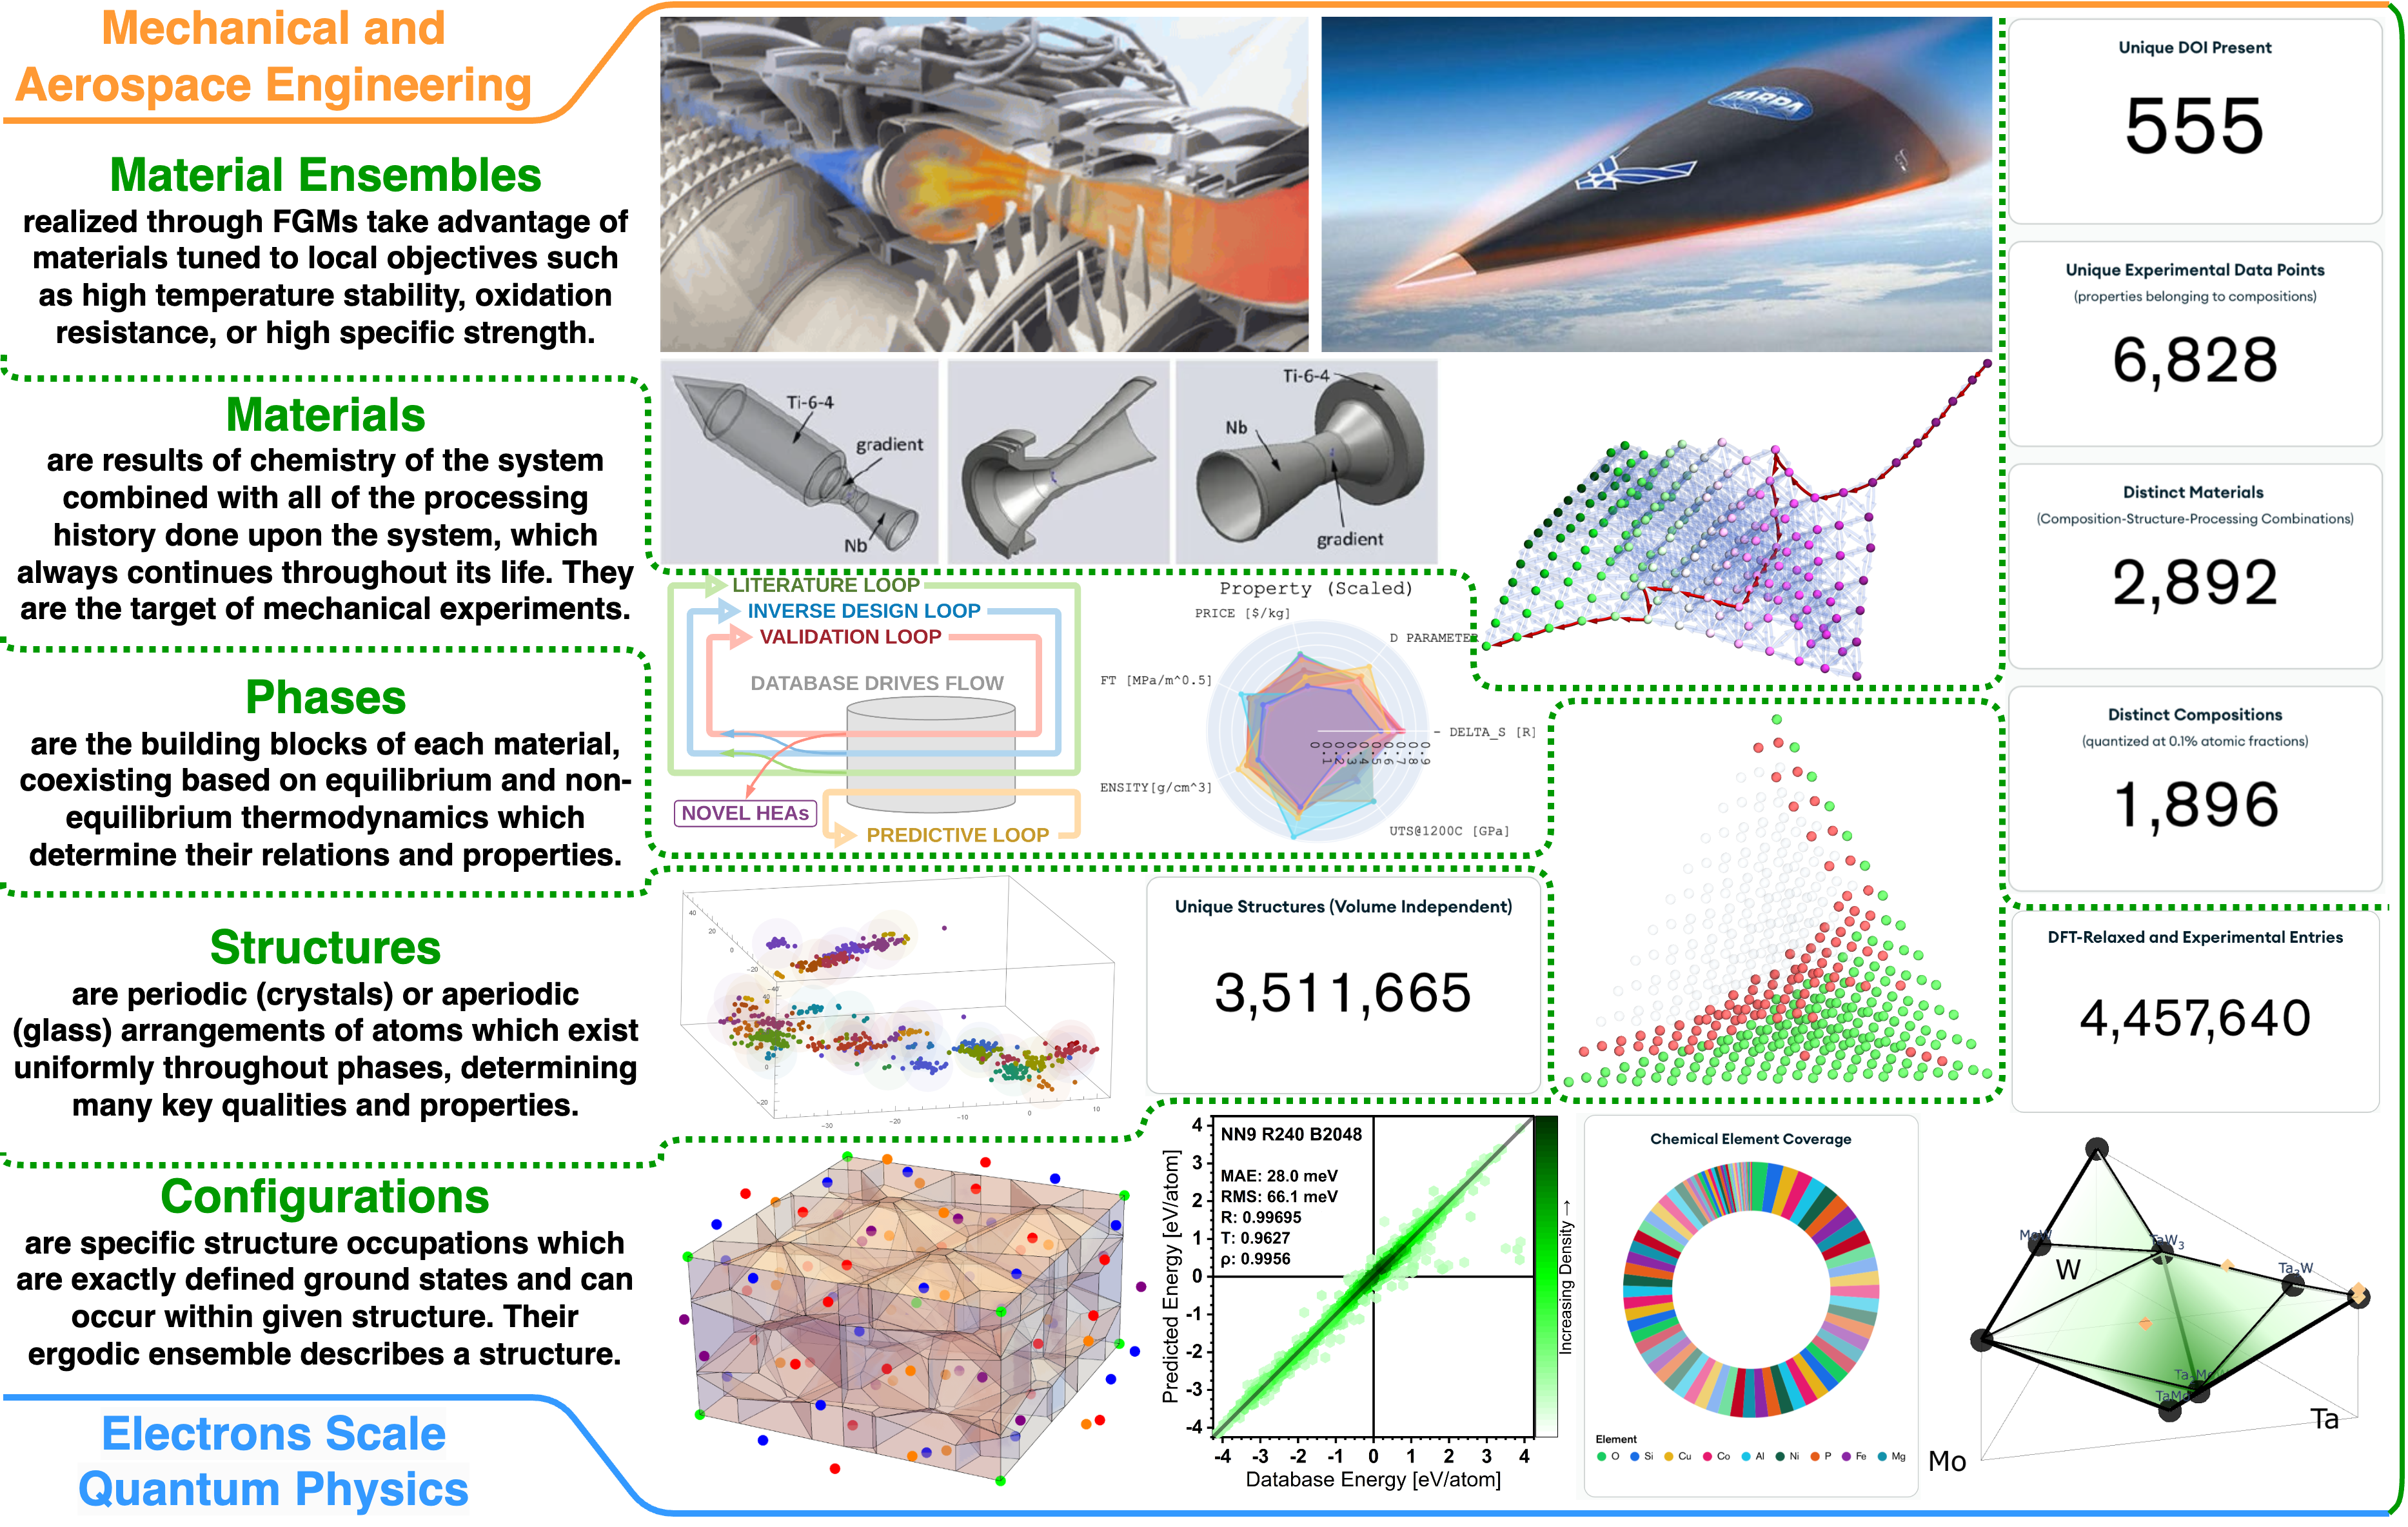
\includegraphics[width=0.95\textwidth]{intro/DissertationBigPicture.png}
    \caption{
    Intermediate material modeling scales bridging together quantum physics and aerospace engineering to enable high-technology solutions through excellence of underlying ensembles of materials. In this work, all of the scales are brought together to take advantage of data and knowledge from all relevant sources. Top render of hypersonic vehicle reproduced from DARPA under public domain and gray nozzle renders from \cite{Hofmann2014DevelopingManufacturing} under CC BY-NC-ND 4.0 License. Several images occur later in the manuscript in Figures \ref{pathplan:fig:lowgradientsquared}, \ref{ultera:fig:dashboard}, \ref{ultera:fig:dataloops}, \ref{inverse:fig:cgandemo}, \ref{infeasibilitygliding:fig:glide}, \ref{crystall:fig:ndbi2clusters}, \ref{pysipfenn:fig:ks2022}, \ref{sipfenn:fig:oqmdperformance}, and \ref{mpdd:fig:dataset}.
    }
    \label{intro:fig:bigpicture}
\end{figure}

Motivation 1:
Per DOE ARPA-E estimates, developing a standalone alloy which could continuously operate at $1300^oC$ has the potential to increase gas turbine efficiency up to 7\%, which will significantly reduce wasted energy and carbon emissions by saving up to 20 quads of energy in electricity generation and civilian aviation between now and 2050 \cite{ULTIMATEArpa-e.energy.gov}. Such efficiency increase could prevent release of approximately 1,000,000,000,000 kg of \ch{CO_2} from burning natural gas, or double that from coal.

Motivation 2:
Another extreme environment application is the class of hypersonic vehicles which travel faster than 5 times the speed of sound \emph{through Earth's atmosphere for extended periods of time}, thus, generating extreme sustained temperatures within structural components. This prompts the need for novel materials and engineering techniques, as evidenced by massive funding assigned to this research areas by United States military which increased its yearly budgets for hypersonic \emph{research} from \$3.8 billion in FY2022, to \$4.7 billion in FY2023, and to an undisclosed amount this year (FY2024) \cite{Sayler2024HypersonicCongress}.

\todo



\section{Flow of Material Discovery and This Work} \label{intro:sec:flow}

Throughout this work, all topics raised in Section \ref{intro:sec:bigpicture} will be discussed in a reversed order to progressively build from fundamentals to highly-specialized final applications, while retaining generality at every stage. This way, one will be able to build a holistic picture focused on how data flows within materials informatics research and converges together at consecutive length-scales to discover new materials in specific niches in a systematic, easy-to-automate approach, rather than build elaborate solutions that may \emph{happen} to work well but can also break the fundamentals - a common occurrence in our era of powerful computing and machine learning where tools \emph{always give an answer} but it may hold negative value.

As shown in Figure \ref{intro:fig:outline}, the first 4 chapters (colored blue) cover atomistic treatment of materials, discussing how data at this level is collected, featurized, managed and expanded. \texttt{SIPFENN} approach and the latest \texttt{pySIPFENN} featurization package are first developed. Then \texttt{MPDD} database with 4.5 million DFT-relaxed or experimentally observed entries is set up to serve as a highly efficient deployment vehicle. Lastly, \texttt{crystALL} approach automatically extends it into chemical areas of interest.

\begin{figure}[H]
    \centering
    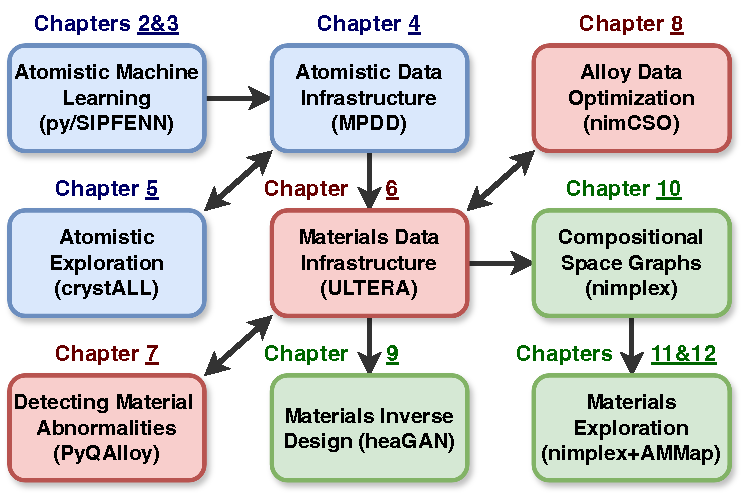
\includegraphics[width=0.7\textwidth]{intro/DissertationOutline.pdf}
    \caption{Schematic outline of this dissertation flowing through 3 overarching types of materials science research. It starts from atomistic treatment (blue) allowing modeling of physical materials (blue) and leading to design (green). For each category, three most significant advancements done in this work have been selected to showcase computational infrastructures and methods to extend our understanding or capabilities.}
    \label{intro:fig:outline}
\end{figure}

All of \texttt{MPDD} is then harvested to model materials at the physical scale by (1) serving as inputs to thermodynamic model generation using \texttt{pycalphad} \cite{Otis2017Pycalphad:Python} and \texttt{ESPEI} \cite{Bocklund2019ESPEICuMg} or training of \texttt{pySIPFENN} ML models generating needed data, and (2) informing experimental observations by, for instance, automatically compiling a set of carbides stable in an alloy system at 0K. At the same time, the largest experimental HEA data infrastructure, called \texttt{ULTERA}, is compiled joining together over 6,800 property datapoints manually extracted from 555 literature publications. 

The experimental database is curated through novel \texttt{PyQAlloy} package created to detect abnormalities and dramatically reduce fraction of erroneous data relative to other similar ones in the literature. Once curated, the \texttt{nimCSO} package can guide ML efforts in terms of which components of the data (chemical elements) should be considered when modeling to optimize trade-off between applicability and data density available to the models




\section{Executive Summary} \label{intro:sec:summary}

%%%%%%%%%%
First, Chapter \fullref{chap:sipfenn} introduces fundamental concepts critical to structure-informed modeling of atomic configurations from the perspective of machine learning (ML) modeling and presents design of such models employing artificial neural networks for the prediction of formation energies of atomic structures based on elemental and structural features of Voronoi-tessellated materials. It provide a concise overview of the connection between the machine learning and the true material-property relationship, how to improve the generalization accuracy by reducing overfitting, how new data can be incorporated into the model to tune it to a specific material system, and preliminary results on using models to preform local structure relaxations.

It results in three final models optimized for achieving (1) highest test accuracy on the Open Quantum Materials Database (OQMD), (2) high extrapolative performance in the discovery of new materials, and (3) high performance at a low computational cost. On a test set of 21,800 compounds randomly selected from OQMD, these models achieves a mean absolute error (MAE) of 28, 40, and 42 meV/atom, respectively. The first model represented the state-of-the-art performance on this problem when released in 2020 \cite{Krajewski2020SIPFENNModels} (see Table \ref{sipfenn:comparison-results}), the second model provides better predictions in a test case of interest not present in the OQMD, while the third one reduces the computational cost by a factor of 8 making it applicable to embedded and mobile applications. A transfer learning procedure was also demonstrated for the first time, showing dramatic improvements in extrapolation with just several datapoints (see Figure \ref{sipfenn:fig:transfersigmaVsDatapoints}).

The results were implemented into a new open-source tool called \texttt{SIPFENN} or \textit{Structure-Informed Prediction of Formation Energy using Neural Networks}, which not only improved the accuracy beyond existing models but also shipped in a ready-to-use form with pre-trained neural networks, which was first-of-a-kind at release, and a GUI interface allowing it be included in DFT calculations routines at nearly no cost.


%%%%%%%%
Next, Chapter \fullref{chap:pysipfenn} expands upon \texttt{SIPFENN} and implements a fully-featured machine learning focused analysis framework called \texttt{pySIPFENN} or \textit{python toolset for Structure-Informed Property and Feature Engineering with Neural Networks} to fuel needs of structure-informed materials informatics - a rapidly evolving discipline of materials science relying on the featurization of atomic structures or configurations to construct vector, voxel, graph, graphlet, and other representations useful for machine learning prediction of properties, fingerprinting, and generative design. This chapter discusses how current featurizers typically perform redundant calculations and how their efficiency could be improved by considering (1) fundamentals of crystallographic (orbits) equivalency to optimize ordered cases and (2) representation-dependent equivalency to optimize cases of dilute, doped, and defect structures with broken symmetry. It also discusses and contrasts ways of (3) approximating random solid solutions occupying arbitrary lattices under such representations.

Efficiency improvements discussed in this work were implemented within \texttt{pySIPFENN} and shown to increase performance from 2 to 10 times for typical inputs just based on fundamentals of materials science. Throughout this work, the authors explicitly discuss how these advances can be applied to different kinds of similar tools in the community.


%%%%%%%
Chapter \fullref{mpdd:sec:mpdd} shifts focus from developing new techniques for data analysis to building an innovative atomistic data infrastructure to fuel machine learning model training and deployment process. This effort builds from the idea that, fundamentally, each atomistic ML study comprises of three elements: a dataset or database of \emph{materials}, a \emph{descriptor} or set of features known for each material, and an ML algorithm trained to predict a \emph{property} or a set of them. These three are combined in two steps. First, the data representation is calculated using the descriptor. Then the model is iteratively evaluated on this representation or adjusted to improve it. Both processes are nearly instantaneous compared to ab-initio based methods; however, with extensive databases or materials modeled with large super-cells (e.g., glasses), compute times can grow into days or years for elaborate analysis tools deployed over many millions of datapoints. 

\texttt{MPDD} is a tool that can speed up the total process for the end-user by orders of magnitude through removal of the most time-intensive step, i.e., the descriptor calculation. To accomplish that, it moves from the traditional practice of sharing only the material-properties data to sharing the descriptors-properties data corresponding to the material as well, employing a high-performance NoSQL \texttt{MongoDB} database with highly engineered indexing system and fully salable compute node deployment model. The latter is used to progressively extend it based on guidance received from tools described in later chapters of this dissertation.

\texttt{MPDD} deployment model is not only much faster but also serves as a tool for an automated and robust embodiment of prior knowledge about materials in a graph-like fashion. Lastly, since the descriptors are often reused for related properties, our database provides a tremendous speed-up in the design space exploration.

Since 2023, a stable, well-implemented endpoint of the \texttt{OPTIMADE} API available at \href{https://optimade.mpdd.org}{https://optimade.mpdd.org} allows \texttt{MPDD} to be seamlessly integrated with other community databases and serve atomistic feature data associated with their entries for synergistic merger of experimental observations, ab initio calculations, and machine learning predictions.


%%%%%%%
Chapter \fullref{chap:crystall}, introduces a simple yet powerful approach to discovery of new atomic structures and identification of experimentally observed ones that evade identification, which was already demonstrated in certain important chemical systems. It implements in a concise computational tool which leverages millions of previously calculated structures from \texttt{MPDD} Database and other databases accessed through the \texttt{OPTIMADE} API to identify all atomic structures that can accommodate target stoichiometry (or uncertain chemical composition form experiments) and perform all permutations of substitutions to arrive at a list of tens of thousands of candidate structures. 

It analyzes candidates in the \texttt{KS2022} feature space, introduced in Chapter \ref{chap:pysipfenn} as part of \texttt{pySIPFENN}, to detect unique set of structures underlying different atomic configurations through different clustering techniques. Lastly, it selects a member from each cluster based on minimum formation energy to arrive at an ensemble of candidate configurations then passed to ab initio calculations or experiments for validation. 

Such ensemble approach is shown to provide critical advantages when contrasted with convex-hull-structure searching approach which recently dominated the community. It can also be used to expand unexplored regions of \texttt{MPDD} database, providing valuable deployment target for machine learning models.


%%%%%%%
Chapter \fullref{chap:ultera} crosses from the atomistic-level materials science into "real" materials physically created and measured experimentally, while still focusing on similar aspects of efficient modeling, data handing, and model deployment. It discusses the \texttt{ULTERA} Database, developed under the ARPA-E's ULTIMATE program and aimed at collecting literature data on high entropy alloys (HEAs).

\texttt{ULTERA} facilitates rapid discovery of new alloys using forward and inverse design, with the primary focus on creep behavior, yield stress, ductility, and hardness. Its advanced architecture, composed of many intermediate databases, pipelines, and analysis tools, is designed to automatically integrate starting literature data in real-time with methods such as experiments, generative modeling, predictive modeling, and validations. Thanks to such automation, the experimental team can operate on the best candidates available, while generation of new ones based on incoming experiments can be delegated to the cloud.

As of April 2024, ULTERA contains over 6,800 property-datapoints, corresponding to 2,900 unique HEAs, manually collected from 550 source literature publications. All data is available through a high-performance API, following FAIR principles.


%%%%%%%
Chapter \fullref{chap:pyqalloy} takes the \texttt{ULTERA} Database and dramatically increases its value to the machine learning applications by removing or fixing approximately 5\% of the errors present in it and other state-of-the-art HEA datasets, arriving at \emph{several times less erroneous data}.

In the past, these challenge was not as severe nor impactfull because the effort placed in the data analysis was much greater than data extraction; however, as our community moves towards this large-scale multi-source data collection, it increasingly starts to surface impacting ML efforts. While present in datasets on all alloy classes, this problem is particularly visible in high entropy alloys (HEAs) due to their novelty and complexity. A number of factors causes errors, including a lack of standardized notations and general parsing mistakes, such as typos, but most of them can be caught through detection of abnormalities in relation to the correct data and its patterns.

In this chapter, we present an open-source Python tool called \texttt{PyQAlloy} that can be run on alloy datasets to screen them for a variety of such abnormalities. It puts each data point in a variety of scopes ranging from individual datapoint analysis, through single-study meta-data, to the database as a whole.


%%%%%%%
Chapter \fullref{chap:nimcso} builds on top of \texttt{ULTERA} datasets curated by \texttt{PyQAlloy} and recognizes that selecting dimensions to model, or in this case, the selection of chemical elements to restrict the modeling effort, is a combinatorically hard problem for complex compositions existing in highly dimensional spaces due to the interdependency of components being present. Consequentially, optimizing the data availability and density for applications such as machine learning becomes a challenge.

A novel tool, called \texttt{nimCSO}, has been introduced and implmenets several methods for performing this task over even millions of datapoints and extreme dimensionalities encountered, for instance, in materials science of Compositionally Complex Materials (CCMs) which often span 20-45 chemical elements, 5-10 processing types, and several temperature regimes, for up to 60 total data dimensions.

It achieves the extreme performance by leveraging the metaprogramming ability of the Nim language to optimize itself at the compile time, both in terms of speed and memory handling, to the specific problem statement and dataset at hand based on a human-readable configuration file. As demonstrated in the chapter, it reaches the physical limits of the hardware (L1 cache latency) and can outperform an efficient native Python implementation over 400 times in terms of speed and 50 times in terms of memory usage (\emph{not} counting interpreter), while also outperforming NumPy implementation 35 and 17 times, respectively, when checking a candidate solution. It was designed to be both a user-ready tool and a scaffold for building even more elaborate methods in the future, including heuristics going beyond data availability. 


%%%%%%%
Chapter \fullref{chap:inversedesign} demonstrates how \texttt{ULTERA} dataset can be used to propose new alloys through inverse design. It leverages conditional Generative Adversarial Netowrks (cGAN) models to bias the predicted alloys in terms of (1) the property values by setting the conditioning and (2) the predicted compositions by recognizing \emph{concept vectors} in the latent space established at the training step. The former ability is implemented within a demonstrator Python package called \texttt{heaGAN} which can be used to design HEAs by setting design criteria. It also allows advanced users to re-train cGAN models based on their own data or a third-party property surrogate model.

%%%%%%%
Chapter \fullref{chap:nimplex} departs from both data and machine learning to focus on the mathematical abstractions of the alloy design problem. It begins by considering that many disciplines of science and engineering deal with problems related to compositions, ranging from chemical compositions in materials science to portfolio compositions in economics. They exist in non-Euclidean simplex spaces, causing many standard tools to be incorrect or inefficient, which is significant in combinatorically or structurally challenging spaces exemplified by Compositionally Complex Materials (CCMs) and Functionally Graded Materials (FGMs). In this chapter, we explore them conceptually in terms of problem spaces and quantitatively in terms of computational feasibility.

Several essential methods specific to the compositional (simplex) spaces are implemented, with most critical parts presented in chapter body as code listings, through a high-performance open-source library \texttt{nimplex}. Most significantly, we derive and implement an algorithm for constructing a novel n-dimensional simplex graph data structure, which contains all discretized compositions and all possible neighbor-to-neighbor transitions as pointer arrays. Critically, no distance or neighborhood calculations are performed, instead leveraging pure combinatorics and the ordering in procedurally generated simplex grids, keeping the algorithm $\mathcal{O}(N)$, so that graphs with billions of transitions take seconds to construct on a laptop. Furthermore, we demonstrate how such graph representations can be combined to express path-planning problem spaces and to incorporate prior knowledge while keeping the problem space homogeneous. This allows for efficient deployment of existing high-performance gradient descent, graph traversal search, and other path optimization algorithms.


%%%%%%%
Chapter \fullref{chap:infeasibilitygliding} leverages the novel graph-based representations of compositional spaces to dramatically improve our approach to screening and modifying compositionally complex alloys based on their structural constraint feasibility. It builds on the fact that the equilibrium existence of a particular phase in the phase-regions of chemical space (not necessarily corresponding to the present elements, as exploted in Chapter \ref{chap:nimplex}) is bound by a continuous surface of (generally) low curvature. Thus, performing the community-standard brute force screening type evaluation of all compositions will often calculate high numbers of points that cannot be reached.

Thus, \texttt{nimplex}-generated graphs are used to quickly re-implement the screening procedure into depth-first search traversals of the feasible regions that \emph{glide one the infeasibility boundaries}, reducing computation by half in semi-randomly picked "bad-case" which was known to produce relatively large feasible regions. In more elaborate screenings not taking advantage of prior knowledge, this improvement may very well reach between one and several orders of magnitude.


%%%%%%%
Lastly, Chapter \fullref{chap:pathplanning} takes additional advantage of the \texttt{nimplex}-generated graphs, which can be also extracted from feasible regions established in \ref{chap:infeasibilitygliding}, to deploy path planning algorithms and find sets of compositions that allow dissimilar alloys to be continuously combined in the least number of steps. Additional considerations are made in relation to an example property field of Root Mean Square Atomic Displacement (RMSAD) related to the yield stress in HEAs. In particular, its value, gradient, and magnitude of gradient are used to modify the graph weights encoding different design objectives, which are effortlessly solved with the same out-of-the box pathfinding approach.


%%%%%%%
Appendix \fullref{chap:supdiscussions} explores minor considerations tangential to the information flow or otherwise less critical, that may be of significant interest to some readers, while Appendix \fullref{chap:othersoft} discusses 8 pieces of software developed to during this work bur (1) were not directly used, (2) critical to discussion, or (3) were a contribution of a component to existing software.

Appendices \fullref{chap:nimplextutorial1} and \fullref{chap:nimplextutorial2} contain workshop material available under \texttt{nimplex} repository adapted to the formatting of this dissertation and go into details of both "Why?" and "How?" tools introduced between Chapters \ref{chap:nimplex} and \ref{chap:pathplanning} can be used by the end user. They can be run interactively with one-click cloud virtual environment by following current link at \href{https://nimplex.phaseslab.org}{nimplex.phaseslab.org} or by running them locally based on the supplementary materials.

Appendices \fullref{chap:pysipfenntutorial1} and \fullref{chap:pysipfenntutorial2} showcase how \texttt{pySIPFENN} integrates with other computational tools in the community and enables one to guide remote DFT calculations on a server cluster and adjust its models to a specific problem. Both were given by Adam Krajewski as guest lectures in the MatSE 580 course at Penn State in the Fall of 2023 and can be run interactively with one-click cloud virtual environment by following current link at \href{https://amkrajewski.github.io/MatSE580GuestLectures}{amkrajewski.github.io/MatSE580GuestLectures}, which also neatly presents the expected outcomes, or by running them locally based on the supplementary materials.

\printbibliography[heading=subbibintoc]

\chapter{Extensible Structure-Informed Prediction of Formation Energy with Improved Accuracy and Usability employing Neural Networks} \label{chap:sipfenn}

\acknowledge{
This chapter adapts verbatim the preprint version of \citet{Krajewski2022ExtensibleNetworks} published under \href{https://arxiv.org/abs/2008.13654v4}{arXiv:2008.13654v4} extended by additional discussions present in earlier versions published starting August 2020 under \href{https://arxiv.org/abs/2008.13654v1}{arXiv:2008.13654v1}. This work was co-authored with Jonathan Siegel, Jinhao-Xu, and Zi-Kui Liu. All text was written by Adam M. Krajewski with Jonathan Siegel co-writing Section \ref{sipfenn:ref:machinelearningoverview}. Jinhao Xu and Zi-Kui Liu provided edits and guidance.
}




\section{Introduction} \label{sipfenn:sec:Introduction}

%\subsection{Motivation} 
\label{sipfenn:ssec:Motivation}
%Introducting paragraph
In recent years the field of material data informatics has been growing in importance thanks to the proliferation of open-access databases \cite{Saal2013MaterialsOQMD,Kirklin2015TheEnergies, vandeWalle2018TheDatabase,Jain2013Commentary:Innovation,Curtarolo2013AFLOW:Discovery,Toher2018TheDiscovery,Pizzi2016AiiDA:Science} and new methods being implemented to predict a wide variety of material properties \cite{Isayev2017UniversalCrystals, Legrain2017HowSolids, Pilania1987MachineSuperlattices, Jung2019BayesianSteels, Ouyang2020ComputationalConductors,Bucior2019Energy-based,Chandrasekaran2019SolvingLearning, Kim2018Machine-learning-acceleratedCompounds,Wen2019MachineProperty, Scime2019UsingProcess}. Within these methods, machine learning (ML) and, more broadly, artificial intelligence (AI) is becoming dominant, as noted in two recent reviews \cite{Schmidt2019RecentScience, Vasudevan2019MaterialsPhysics}, which listed a total of around 100 recent studies that attempted to solve material science problems using ML and AI techniques. These studies report benefits such as a 30-fold increase in material discovery rate when guided by an ML-model \cite{Kim2018Machine-learning-acceleratedCompounds}, or the ability to create new state-of-the-art materials in highly complex design spaces like 6-component alloys \cite{Wen2019MachineProperty}. They also dive into new paradigms of materials science by handling previously unthinkable amounts of data, allowing the creation and analysis of an energy convex-hull calculated for all elements \cite{Aykol2019NetworkDiscovery, I.Hegde2020TheMaterials}, or a concurrent analysis of all available literature texts to find paths for material synthesis \cite{Kononova2019Text-minedRecipes}. In addition, some studies promise to solve significant industrial challenges such as detection of additive manufacturing flaws with relatively simple and accessible data, but above-human pattern recognition quality and speed \cite{Scime2019UsingProcess}.

%Materials Discovery & Materials Stability 
A common approach is to  focus on the discovery of candidate materials promising a new state-of-the-art performance, which must then be validated by experiment. The mismatch between the predictions and experiment measures the quality of the model, and reducing this gap is a major challenge due to the newly designed materials often being far from known materials, combined with attention placed on regions with extraordinary predictions.However, even if design models were perfectly accurate, many predicted materials cannot be physically made in the lab. An increasing number of studies attempt to solve this challenge by focusing not only on predicting how the material will perform but also on whether it can be manufactured \cite{Alberi2019TheRoadmap}. Generally, these include predicting materials' stability \cite{Balachandran2018PredictionsTheory, Li2019ThermodynamicLearning, I.Hegde2020TheMaterials, Im2022ThermodynamicModeling, Shang2021FormingJoints} and synthesizability \cite{Hattrick-Simpers2018AMaterials,Kononova2019Text-minedRecipes, Aykol2019NetworkDiscovery} with the stability being the more constraining parameter, as it determines whether the material could be stable or metastable in the use conditions, and therefore whether it can be synthesizable. Thus, predicting stability through prediction of fundamental thermodynamic properties such as formation energy is of special importance.

%Machine Learning:
In the present work, new ML models and a tool to quickly use them are developed to improve the process of materials discovery by efficient prediction the formation energy and streamlined incorporation into materials discovery frameworks that aim to screen billions rather than hundreds of candidates available with cost-intensive calculations like first-principles calculations based on the density functional theory (DFT). 

%\subsection{Machine Learning Approach}
\label{sipfenn:ssec:currentapproach}
In simple terms, every ML model is composed of three essential elements: a database, a descriptor, and an ML technique (also known as ML algorithm). The first element, databases, contain prior knowledge and are becoming increasingly shared between many studies, thanks to being open-access and often containing orders of magnitude more experimental or computational data than could be feasibly collected for a single study \cite{Saal2013MaterialsOQMD,Kirklin2015TheEnergies, vandeWalle2018TheDatabase,Jain2013Commentary:Innovation,Curtarolo2013AFLOW:Discovery,Toher2018TheDiscovery,Pizzi2016AiiDA:Science}. Databases used within the present paper are detailed in Section \ref{sipfenn:sssec:Data}.

The second element of an ML model is the descriptor (i.e., feature vector describing the material) which determines a representation of knowledge (data from the database) in a way relevant to the problem. It is typically built from many features, also known as attributes or vector components, which usually are determined through domain knowledge to be relevant or selected through correlation analysis. All combined, these features are a representation of some state whose meaning will be problem-specific.

When treating materials on the single atomic configuration level, descriptors can be generally divided into composition-based (also known as stoichiometric, structure-invariant, or elemental) \cite{Jha2018ElemNet:Composition, Ward2016AMaterials, , Legrain2017HowSolids} and structure-informed \cite{Ward2017IncludingTessellations, Seko2017RepresentationProperties,Schutt2014HowProperties}. The first type usually provides a more compact representation at a much lower computational cost, as calculating a composition-based descriptor often needs to involve only simple linear algebra operations such as matrix multiplication \cite{Ward2016AMaterials}, or prior-knowledge-incorporating attention-based analysis of a graph representation of the composition \cite{Goodall2020PredictingStoichiometry}. In cases where deep neural networks (DNNs) are employed, descriptor calculation can be skipped altogether by passing a composition vector directly \cite{Jha2018ElemNet:Composition}.

It is important to recognize that the descriptor choice impacts both the performance and applicability of the model. In the case of prediction of material properties, such as formation energy, selecting a composition-based descriptor, no matter how complex, limits the model to either a specific arrangement of atoms, such as BCC or amorphous, or some defined pattern of structures, such as the convex hull of lowest-energy structures. Such limitation of the problem domain, given a comparable amount of data, allows to quickly achieve much lower prediction error at a cost of fundamentally changing the problem, making a comparison between methods impossible. Furthermore, a composition-only representation is inherently unsuitable for the direct prediction of most material properties that depend on the atomic structure. The structure-informed descriptors can include much more information related to interatomic interactions, making them more robust and more physics-relevant. They also, implicitly or explicitly, include symmetries present in the material, which can be used to predict certain properties, such as zero piezoelectric response, with high confidence. Furthermore, such descriptors often include extensive composition-based arguments within them \cite{Ward2017IncludingTessellations}, making it possible to both recognize patterns in the property coming from different chemical species occupying the same structure and structural effects in the case of a single composition.

At the same time, it is important to consider that physically existing materials are rarely described by a single atomic configuration, usually requiring considerations for defects and coexisting configurations. Thus, like a traditional DFT-based modeling, in order to reproduce real material behavior, a structure-informed model will often require utilization of a method such as CALPHAD \cite{Kaufman1970ComputerMetals, Liu2018OceanLearning}. One of such methods, recently developed by authors and named "zentropy theory" shows the potential to connect individual configurations to predict macroscopic properties, such as colossal positive and negative thermal expansions \cite{Liu2022ZentropyExpansion}.

In some cases however, investigating all configurations can be a very challenging task (e.g., for high entropy alloys), necessitating the use of an elemental-only model trained to give predictions assuming future observations to be consistent with the past ones \cite{Debnath2021GenerativeAlloys}. 

%\subsection{the present work Approach}
\label{sipfenn:ssec:specificapproach}
%\textbf{\textcolor{red}{Need to rework citations to new structure of Methods.}}\\

The structure-informed representation which was the ground for the present work has been developed by Ward et al. based on information from the Voronoi tesselation of a crystal structure \cite{Ward2017IncludingTessellations}. Ward's descriptor contains 271 features that combine information from elemental properties of atoms, such as shell occurrences, with information about the their local environments, such as coordination number or bond lengths to neighbours. This approach was demonstrated to work excellently when comprehensively compared to two previous approaches based on the Coulomb matrix (CM) \cite{Schutt2014HowProperties} and on the partial radial distribution function (PRDF) \cite{Seko2017RepresentationProperties}, when trained on the same data from the Open Quantum Materials Database (OQMD) and with the same machine learning algorithm. A more detailed overview is given in \ref{sipfenn:ssec:descriptorused}.

Ward et al. used an automated Random Forest ML algorithm \cite{Ward2017IncludingTessellations} set to a fully automatic parameter selection. While fairly common, that approach without complexity limit for the model, and when trained on over 400,000 materials, resulted in a forest composed of 100 trees with approximately 700,000 nodes each. Such model requires over 27 GB of RAM memory to run, making it unusable on a typical personal or lab computer. Such size also results in a relatively low efficiency, requiring over 100 ms to run on a high-performance lab computer \cite{Ward2017IncludingTessellations}.

In the present work, aforementioned issues are resolved through a targeted design of the ML algorithm to fully utilize the data and its representation. This is done by consideration of the problem formulation and the deep neural network technique (see \ref{sipfenn:ref:machinelearningoverview}), combined with iterative model design (see \ref{sipfenn:sssec:NetDesign}), and by designing and testing over 50 neural networks belonging to around 30 designed architectures. Notably, in the time between Ward's work and the present paper, neural networks have been used in this application, e.g., \cite{Jha2019IRNet}, which uses residual neural networks. However, as we show in Section \ref{sipfenn:ssec:oqmdperformance}, the present paper provides more accurate predictions than both Ward's model and the state-of-the-art neural network model \cite{Jha2019IRNet}.

Additionally, the present work brings two further improvements. The first one is good transfer learning ability, described in \ref{sipfenn:ssec:transferlearningresults} allowing other researchers, at a relatively small cost, to adjust the model to small problem-specific databases, typically consisting of tens of DFT calculations or less. This method substantially improves predictions for similar materials while retaining the general knowledge learnt from the large data set and demonstrates that the model learns features related to underlying physics. The second  improvement is the end-user usability. While most of the materials-related ML model are reported in a reproducible way with an evaluation of the performance \cite{Ward2017IncludingTessellations, Schutt2014HowProperties, Schutt2018SchNetMaterials, Seko2017RepresentationProperties}, only a fraction goes beyond to make models accessible to the community. the present work has been focused on creating a Findable, Accessible, Interoperable, and Reusable tool, inspired by FAIR principles \cite{FAIRFAIR}, created open-source with common and convertible data formats as is described in more detail in \ref{sipfenn:sssec:SoftwareUsed}. This lead to many standalone components combined into an end-user tool, described in \ref{sipfenn:ssec:SIPFENN}, that is ready to use without any costly computation to create the model and can be run on any modern computer, as low-power as smartphones.

\section{Methodology} \label{sipfenn:sec:methodology}

\subsection{Descriptor Used} \label{sipfenn:ssec:descriptorused}
A descriptor of a material is a point in a well-defined multidimensional property space that can be used to represent knowledge associated with entries in a database in vector form. Within the present work, the property space has 271 dimensions (corresponding to 271 features) related to elemental properties and atomic structure of an arbitrary crystalline material, as designed by Ward et al. \cite{Ward2016AMaterials, Ward2017IncludingTessellations} utilizing the \texttt{voro++} code \cite{rycroft2009voro++}. These features can be categorized as:

\begin{itemize}
    \item \textbf{Elemental Attributes} (145 total): Attributes which only depend upon the elements present and their stoichiometry.
    \begin{itemize}
        \item \textbf{Stoichiometric Attributes} (6): Describe the components fractions.
        \item \textbf{Elemental Properties Attributes} (132): Contain statistics taken over the various elemental properties, weighted by the stoichiometry of the structure.
        \item \textbf{Attributes based on Valence Orbital Occupation} (4): Depend upon the distribution of valence electrons across different orbitals, i.e. on the total number of valence electrons in each orbital across the structure.
        \item \textbf{Ionic Character Attributes} (3): Attributes which encode whether the material is ionically bonded. 
    \end{itemize}
    \item \textbf{Structural Attributes} (126 total): Attributes which depend on the precise structural configuration, i.e. exactly how the atoms are arranged in space.
    \begin{itemize}
        \item \textbf{Geometry Attributes} (16): Attributes which depend upon the spatial configuration of atoms only.
        \item \textbf{Physical Property Differences Attributes} (110): Contain statistics taken over the differences between elemental properties of neighboring sites in the structure, weighted by the size of the Voronoi cell face between the neighbors.
    \end{itemize}
\end{itemize}

A complete table list of features is given in Table \ref{sipfenn:feature-table}. Further details can be found in \cite{Ward2016AMaterials, Ward2017IncludingTessellations}.

\begin{table}[H]
    \footnotesize
    \centering
    \caption{List of Features with Descriptions. Site Statistics refers the mean, range, mean absolute error, maximum, minimum, and mode unless otherwise stated in the description. Difference Statistics refers to the mean, mean absolute error, minimum, maximum and range of the differences between neighboring sites in a structure, weighted by the size of the face between them in the Voronoi tessellation.}
    \begin{tabular}{|p{2.25cm}|p{2cm}|c|c|}
        \hline
        \textbf{Site \hspace{0.3cm} Statistics} & \textbf{Difference \hspace{0.3cm} Statistics} & \textbf{Name} & \textbf{Description} \\
        \hline
        1-4 & - & Effective Coordination Number & mean, mean abs error, min, max\\
        \hline
        5-7 & - & Mean Bond Length & mean abs error, min, max\\
        \hline
        8-11 & - & Bond Length Variation & mean, mean abs error, min, max \\
        \hline
        12 & - & Cell Volume Variation & Variation in the voronoi cell volume\\
        & & & no statistics \\
        \hline
        13-15 & - & Mean WC Magnitude & shells 1-3, global non-backtracking \\
        \hline
        16 & - & Packing Efficiency & no statistics \\
        \hline
        133-138 & 17-21 & Atomic Number & \\
        \hline
        139-144 & 22-26 & Mendeleev Number & \\ 
        \hline
        145-150 & 27-31 & Atomic Weight & \\ 
        \hline
        151-156 & 32-36 & Melting Temperature & \\ 
        \hline
        157-162 & 37-41 & Column & Group in Periodic Table \\ 
        \hline
        163-168 & 42-46 & Row & Period in Periodic Table\\ 
        \hline
        169-174 & 47-51 & Covalent Radius & \\ 
        \hline
        175-180 & 52-56 & Electronegativity & \\ 
        \hline
        181-210 & 57-81 & Valence Electron Count & Listed for s,p,d,f orbitals and total \\ 
        \hline
        211-240 & 82-106 & Unfilled Count & Number of unfilled orbitals \\
         & & & Listed for s,p,d,f orbitals and total \\
         \hline
        241-246 & 107-111 & Ground State Volume & \\ 
        \hline
        247-252 & 112-116 & Ground State Band Gap & \\ 
        \hline
        253-258 & 117-121 & Ground State Magnetic Moment & \\ 
        \hline
        259-264 & 122-126 & Space Group Number & Index of Space group\\
        \hline
        127 & - & Number of Components & no statistics \\
        \hline
        128-132 & - & $\ell^p$-norms of Component Fractions & $p \in \{2,3,5,7,10\}$ \\
        \hline
        265-268 & - & Fraction of Valence Electrons & \\
        & & in s,p,d,f orbitals & no statistics\\
        \hline
        269 & - & Can Form Ionic Compound & boolean, no statistics\\
        \hline
        270-271 & - & Ionic Character & max, mean over pairs of species\\
        \hline
    \end{tabular}
    \label{sipfenn:feature-table}
\end{table}

\subsection{Machine Learning Techniques Overview} \label{sipfenn:ref:machinelearningoverview}
This section gives a brief overview of the employed machine learning techniques and terminology, described in more detail in the Appendix \ref{sipfenn:appedix1}. The interest is placed on the statistical problem of regression, whose goal is to learn a functional relationship $f:X\rightarrow Y$ which minimizes the risk (also known as loss or expected error) \cite{vapnik1999overview} given by

\begin{equation} \label{sipfenn:true_risk}
    R(f) = \mathbb{E}_{x,y\sim \mathcal{P}} l(y,f(x)).
\end{equation}

Here $X$ denotes a space of input features, $Y$ denotes an output space, the expectation above is taken over an unknown distribution $\mathcal{P}$ on $X\times Y$ (representing the true relationship between inputs and outputs), and $l$ is a given loss function. 

In the specific application considered here, the function $f$ which is to be learned, maps input material structures (arrangements of atoms) $x$ to the predicted formation energy $y$. The distribution $\mathcal{P}$ is unknown, but samples $(x_i,y_i)$ are given, consisting of structures $x_i$ and corresponding predictions $y_i$ which are used to learning $f$. In the present case, this data comes from the OQMD and other smaller materials databases.

% \begin{figure}[h]
%     \centering
%     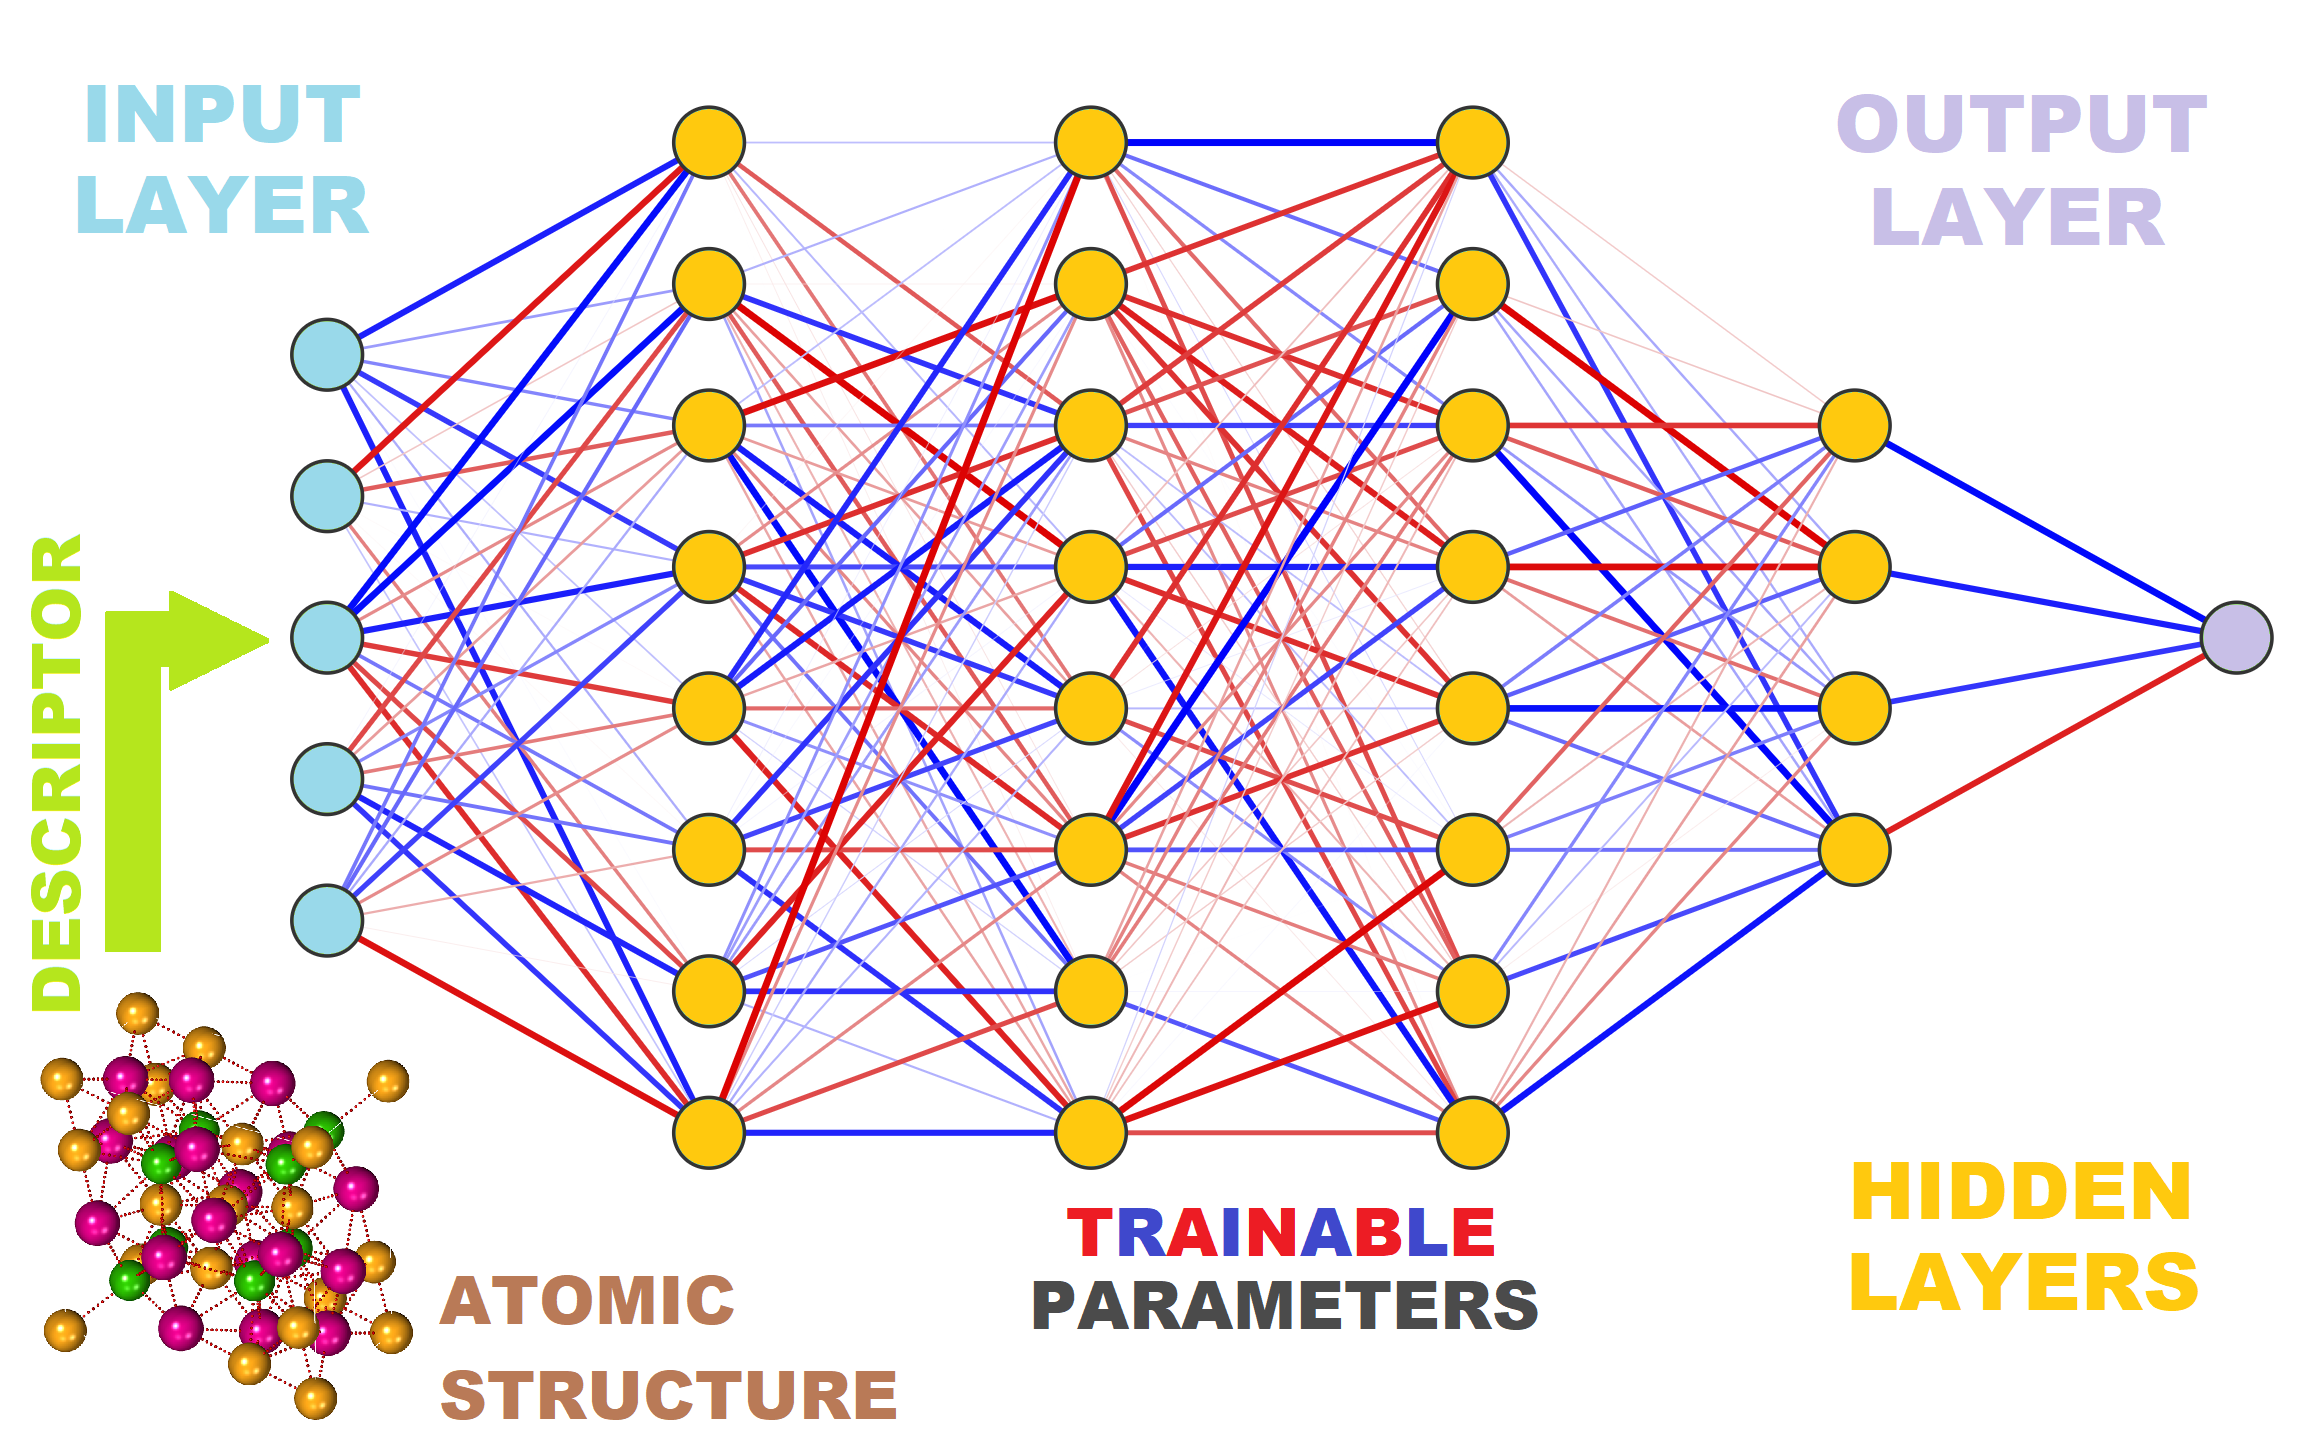
\includegraphics[width=0.65\textwidth]{sipfenn/neuralnetcolorized_V4.png}
%     \caption{Simplified artificial neural network schematic}
%     \label{sipfenn:fig:nnschematic-body}
% \end{figure}

In order to learn the relationship $f$ from the data, the empirical risk

\begin{equation} \label{sipfenn:empirical_risk}
    L(f) = \frac{1}{n}\displaystyle\sum_{i=1}^n l(y_i, f(x_i)),
\end{equation}

is minimized over a class of functions defined by a neural network architecture. A neural network architecture consists of a sequence of alternating linear functions and point-wise non-linear functions defined by an activation function (see \cite{goodfellow2016deep} for more information about neural networks). As the loss function $l$ in \eqref{sipfenn:empirical_risk} the $\ell^1$-loss function $l(y,x) = |x-y|$ is used. The neural networks are trained on this loss \eqref{sipfenn:empirical_risk} using the common ADAM optimizer \cite{kingma2014adam}. 

An important issue when training complex statistical models is the overfitting, which occurs when a model accurately fits the training data but fails to generalize well to new examples. In order to detect overfitting, the standard practice of dividing the data into training, validation, and test datasets \cite{hastie2009elements} is used. In order to mitigate overfitting, dropout \cite{srivastava2014dropout} and weight decay, two standard methods for regularizing neural networks, are used. In Section \ref{sipfenn:sssec:DesignedModels}, Figure \ref{sipfenn:fig:trainingvalidation-body} illustrates overfitting mitigation effects on the training process of neural networks designed in the present paper.

\subsection{Software Used} \label{sipfenn:sssec:SoftwareUsed}

The choice of software for the machine learning portion of \texttt{SIPFENN} was Apache \texttt{MXNet} \cite{ChenMXNet:Systems} due to it's open source nature, model portability, and state-of-the-art scalability, allowing the same code to run on a laptop with a low-power CPU/GPU and a supercomputer (e.g., ORNL Summit) with hundreds of powerful GPU's. It's portability allows trained networks to be converted and used with other popular frameworks such as Google \texttt{Tensorflow}, \texttt{PyTorch}, or even Apple's \texttt{Core ML}, making results of the present paper highly accessible.

\texttt{MXNet} framework was used through \texttt{Wolfram} and \texttt{Python} languages. \texttt{Wolfram} language was used primarily for the network architecture design, training, and testing, as it provides an excellent interface with detailed training results shown in real-time during the training process. It also provides good out-of-the-box performance due to its well-optimized memory handling when training on a single GPU setup. 

Python, on the other hand, was used when writing the end-user tool for running previously trained networks. This choice was made so that the software is completely open-source and can be easily reused for specific purposes or incorporated within other packages. Furthermore, Python allowed quick implementation of a Graphical User Interface (GUI) through the \texttt{wxpython package}.

As explored later in Chapter \ref{chap:pysipfenn}, over several years, the software evolved and developed into \texttt{pySIPFENN} framework which, as of April 2024, has moved to \texttt{PyTorch} for ML runtime and Open Neural Network Exchange (\texttt{ONNX}) format \cite{Bai2019ONNX:Exchange} for model storage and distribution.

\subsection{Data Acquisition and Curation} \label{sipfenn:sssec:Data}

Four sets of data were used within the present work. The largest by volume and significance was the Open Quantum Materials Database (OQMD) \cite{Kirklin2015TheEnergies, Saal2013MaterialsOQMD, Shen2022ReflectionsOQMD}, which contains the results of DFT calculations performed by the Vienna Ab Initio Simulation Package (VASP) \cite{Kresse1993AbMetals} for a broad spectrum of materials. The snapshot used here was extracted from the database by Ward et al. in 2017 and contained 435,792 unique compounds \cite{Ward2017IncludingTessellations}. The choice of 2017 snapshot rather than the current one was made to ensure direct performance comparison between new and previously reported methods. The second database was a part of the Inorganic Crystal Structure Database (ICSD), a subset of the OQMD with only experimentally obtained structures containing around 30,000 entries. ICSD was primarily used for the quick design of simple neural network architectures at the beginning, and OQMD used for more complex models designed later. 

Two smaller data sets were used, in addition to these large databases. The first small dataset contained DFT-calculated formation energies of Fe-Cr-Ni ternary $\sigma$-phase endmembers in the 5-sublattice model \cite{Feurer2019Cr-Fe-NiCalculations}. As this model contains 5 chemically distinct positions (Wyckoff positions), populated by one of 3 elements, in total it included 243 ($3^5$) structures with 30-atom basis each. This data served as an example of a relatively complex structure that was not included in the OQMD. Furthermore, it was a test case of a material that is highly industry-relevant, as it causes steel embrittelment \cite{Hsieh2012OverviewSteels} and is costly to investigate using traditional methods due to compositional and configurational complexity. The second small dataset included 13 Special Quasirandom Structures (SQS), which are the best periodic supercell approximations to the true disordered state of metal alloys \cite{Zunger1990SpecialStructures, Jiang2004First-principlesStructures, Shin2006ThermodynamicStructures}. SQS structures in this set were binary alloys containing Fe, Ni, Co, and V, laying on deformed FCC (A1), BCC (A2), or HCP (A3) lattices. The main purpose of these smaller datasets was to test the performance in extrapolation from OQMD, in a particular case of interest for the author's.

During the network design process described in \ref{sipfenn:sssec:NetDesign}, it was found that a small fraction of the OQMD dataset (under 0.03\%) contains anomalous values of formation energy above 10 eV/atom. In the extreme case of $CuO_2$ (OQMD ID: 647358) this value was 1123 eV/atom or 108350 kJ/mole. Since the source database contains hundreds of thousands of data points reported by many scientists, it can be expected that a small fraction of the data may contain some sort of errors and typos. In the present work, they were removed from all datasets used for training and evaluation.

\subsection{Neural Network Design Process} \label{sipfenn:sssec:NetDesign}

This section conceptually outlines the network design process leading to the final models. All essential details regarding the design and performance of intermediate models, useful for better understanding changes and for applying the similar approach in different problems, can be found in the Appendix \ref{sipfenn:appendix2}.

The design started with the simplest single-layer neural network (perceptron) with the Sigmoid activation function, trained on the ICSD and its smaller subset, to provide a baseline for the design. Then, the process was conducted in the following steps:

    \begin{figure}[H]
    \centering
    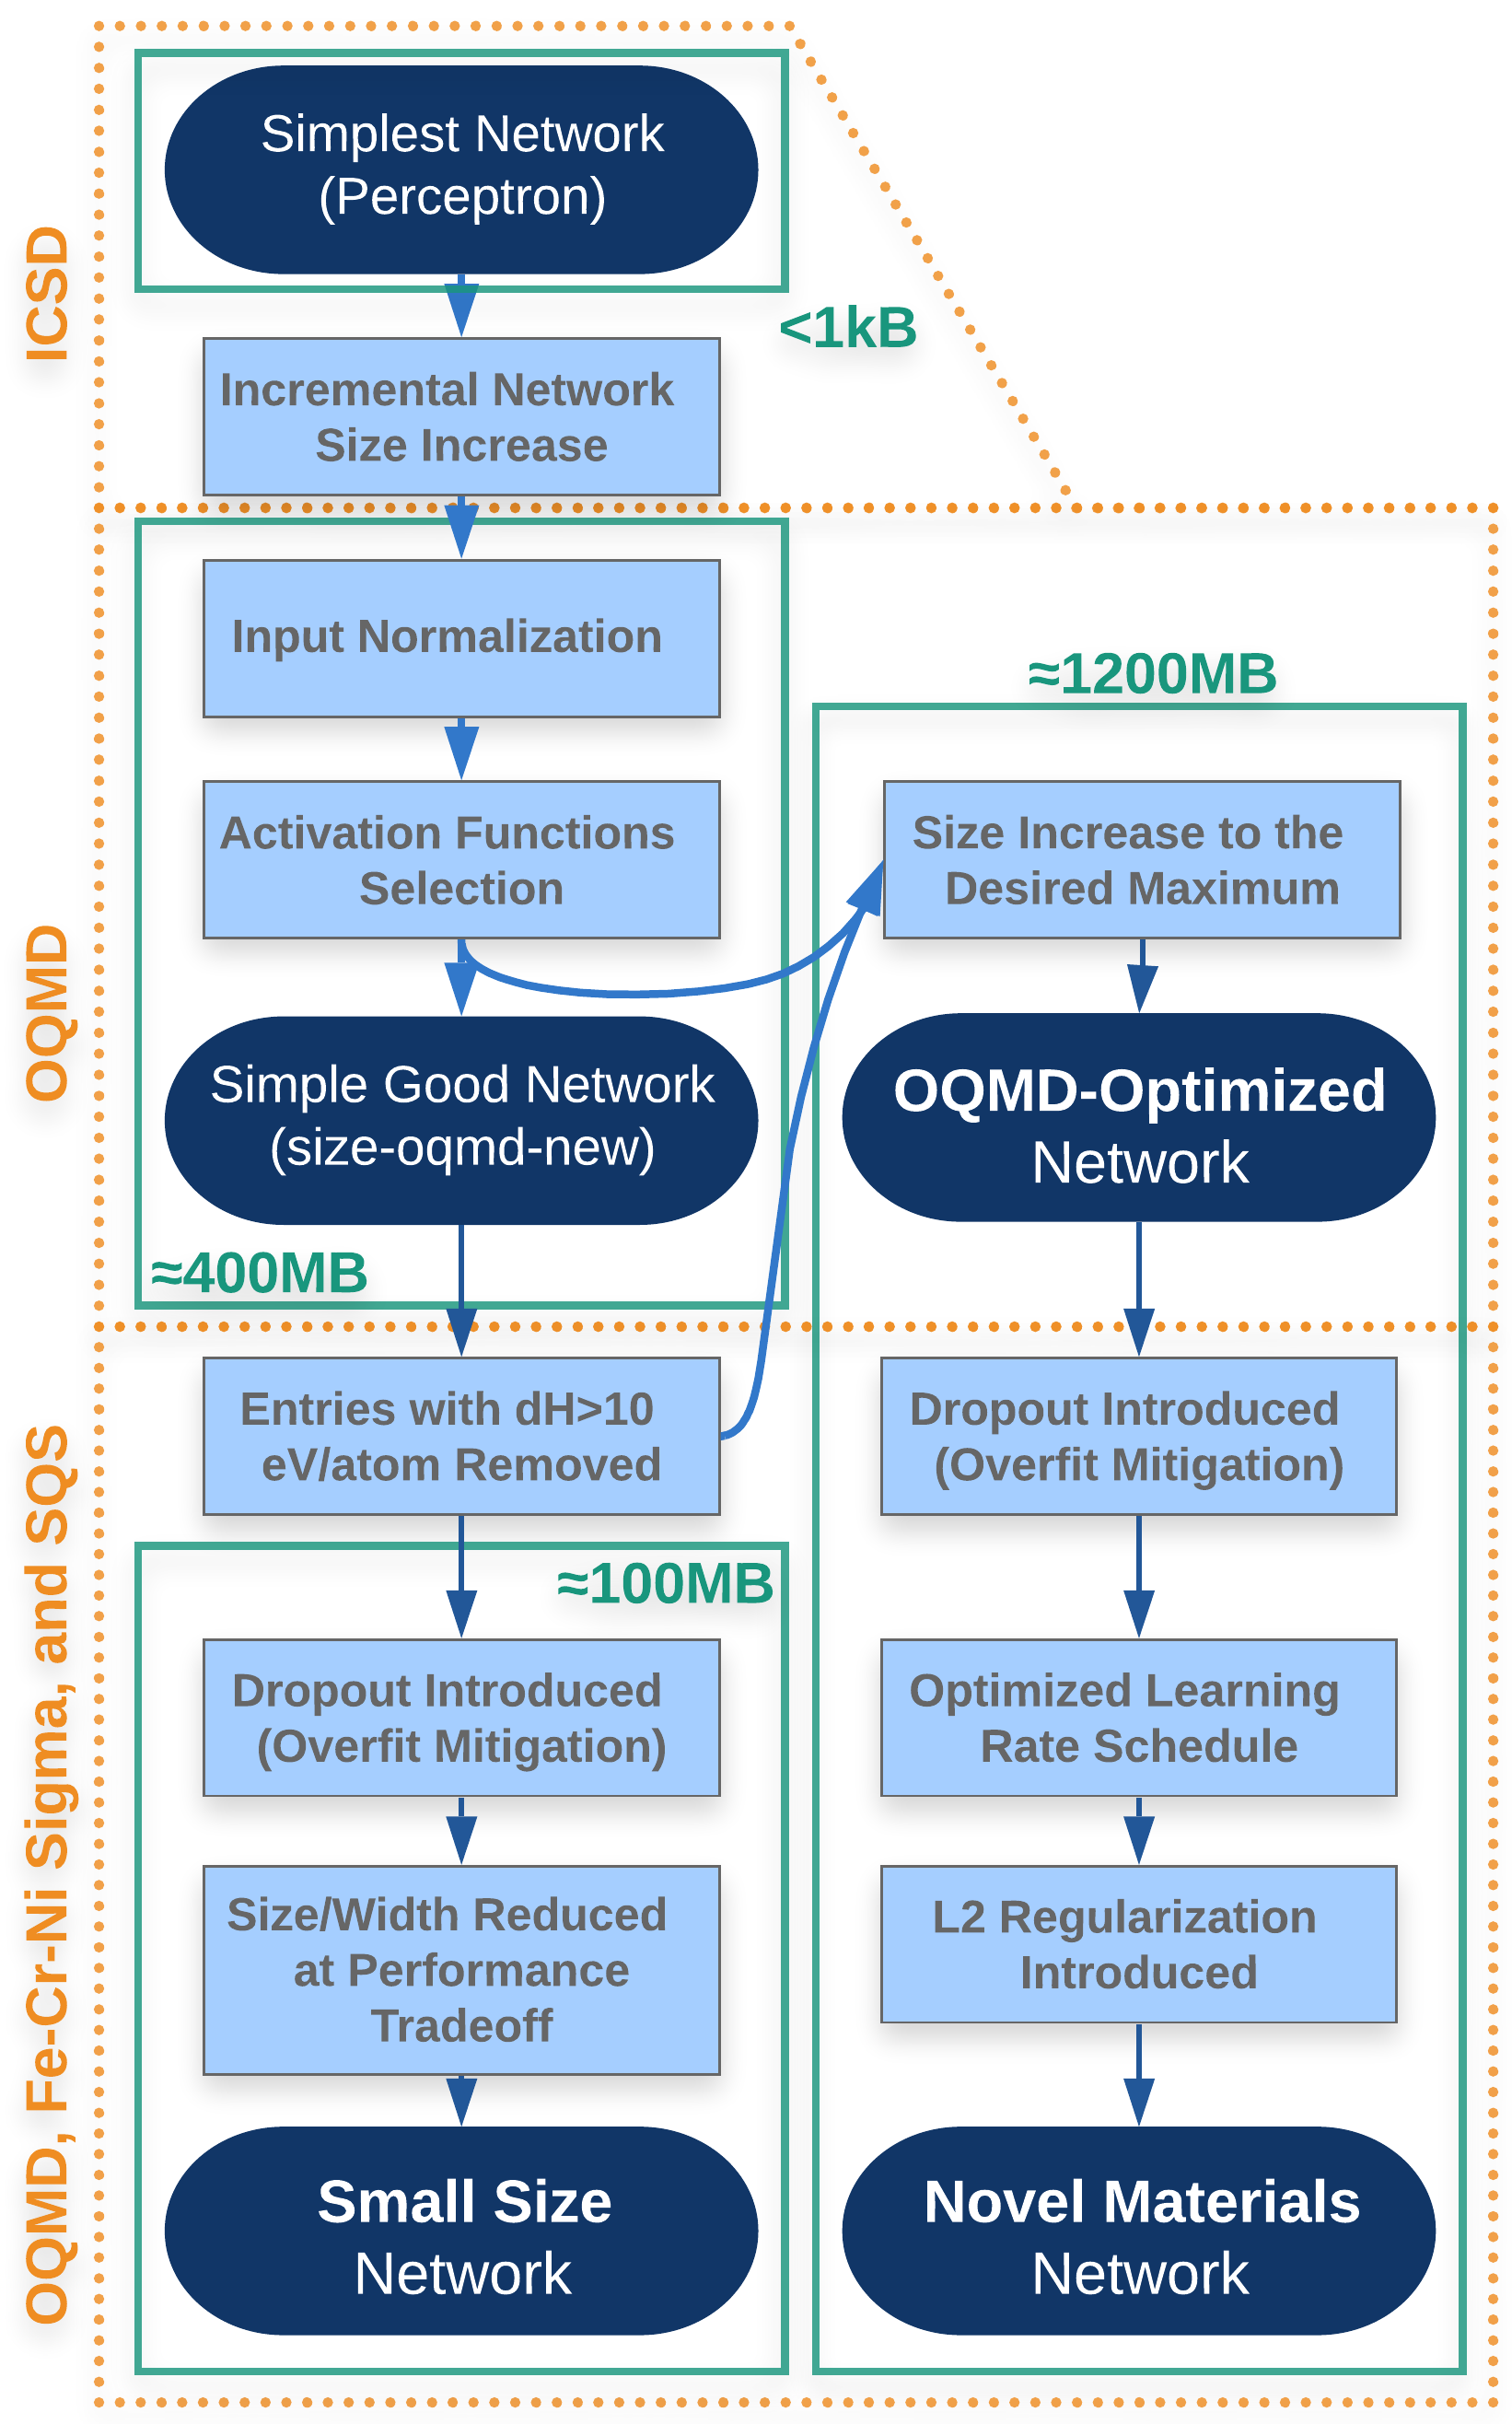
\includegraphics[width=0.56\textwidth]{sipfenn/SIPFENN_design_updated.png}
    \caption{The model design process schematic.}
    \label{sipfenn:fig:designprocess}
    \end{figure}

\textbf{1. }The network size has been increased step-wise while training on the ICSD dataset (30k+ entries). Results were extrapolated to estimate network size suitable for larger OQMD (400k+) to be 4 hidden layers in a (10000, 10000, 1000, 100) configuration.

\textbf{2. }To improve convergence during the training, descriptor features values were normalized to their maximum values present in the OQMD dataset.

\textbf{3. }Performance and time to convergence were improved by moving from Sigmoid activation function to a mix of Soft Sign, Exponential Linear Unit, and Sigmoid. This relatively simple model has improved performance over the existing Random Forest model \cite{Ward2017IncludingTessellations}, achieving MAE of 42 meV/atom on the same dataset.

\textbf{4. }At this step, it was noticed that a small fraction (around 0.03\%) of data points exhibits extreme errors, as high as over 1,000,000 meV/atom causing some instability during the training process, despite the large batch size of 2048. They also caused a high deviation in test MAE values across repeated model training rounds. As describes in \ref{sipfenn:sssec:Data}, these were identified to be a few rare errors in the dataset and removed during later model design. 

\textbf{5. }The network size was increased to around 1GB limit (maximum size target) by the addition of two more 10,000-width layers. This \textbf{OQMD-optimized} network has achieved the best performance on the OQMD out of all designed in the present paper, with an MAE of 28 meV/atom. Performance analysis can be found in \ref{sipfenn:ssec:oqmdperformance} and in Figure \ref{sipfenn:fig:oqmdperformance}.

\textbf{6. }After the good performance on the OQMD was achieved, the design goals shifted to (1) reducing the training-set-to-validation-set error mismatch during the network training, while (2) keeping the test MAE on the OQMD on a suitable level (below 50 meV/atom), and (3) improving performance on datasets not presented to network before (see \ref{sipfenn:sssec:Data}). The first step was the introduction of Dropout layers\cite{srivastava2014dropout}, described in more detail in Appendix \ref{sipfenn:appedix1}, which allow for better distribution of knowledge across the network.

\textbf{7. }The introduction of strong Dropout\cite{srivastava2014dropout} made the network prone to falling in local minima, which was solved by the introduction of a changing learning rate schedule.

\textbf{8. }With optimized network architecture, lastly, the descriptor interpretation by the network has been modified through the introduction of L2 regularization \cite{L2Regularization}, a technique which assigns an error penalty for "attention" (input layer weights) to each of the descriptor features, effectively refining features in the descriptor to only the most significant ones. Figure \ref{sipfenn:fig:squaredweights} ranks them. The resulting \textbf{Novel Materials} model achieved a much lower training-set-to-validation-set error mismatch (1.15 vs 1.57 after 240 rounds), presented in Figure \ref{sipfenn:fig:trainingvalidation} as a function of training progress. On the OQMD test set, it achieved a higher, yet suitable 49 meV/atom.

\textbf{9. }To cater to applications requiring very high throughput or low memory consumption, an additional \textbf{Small Size} network was designed by adding Dropout to one of the earlier networks, designed before the size increase step, and then reducing its size to the desired level. It was found that after reduction of total size from around 400MB to around 100MB, the network retained MAE of 42 meV/atom on an OQMD test set and further reduction was possible if needed for the application.

\section{Results} \label{sipfenn:sec:Results}

\subsection{Final Predictive Models} \label{sipfenn:sssec:DesignedModels}

Throughout the architecture design process described in \ref{sipfenn:sssec:NetDesign}, detailed in Appendix \ref{sipfenn:appendix2}, and depicted in Figure \ref{sipfenn:fig:designprocess}, new networks were designed and tested in various ways, leading to about 50 predictive models (trained neural networks) with varying training parameters and training data. The majority of the intermediate networks were stored for the record, and are available upon request. Details regarding hyper-parameters and training routines used to obtain three resulting models can be found in the Appendix \ref{sipfenn:appedix1}.

\begin{figure}[H]
    \centering
    \frame{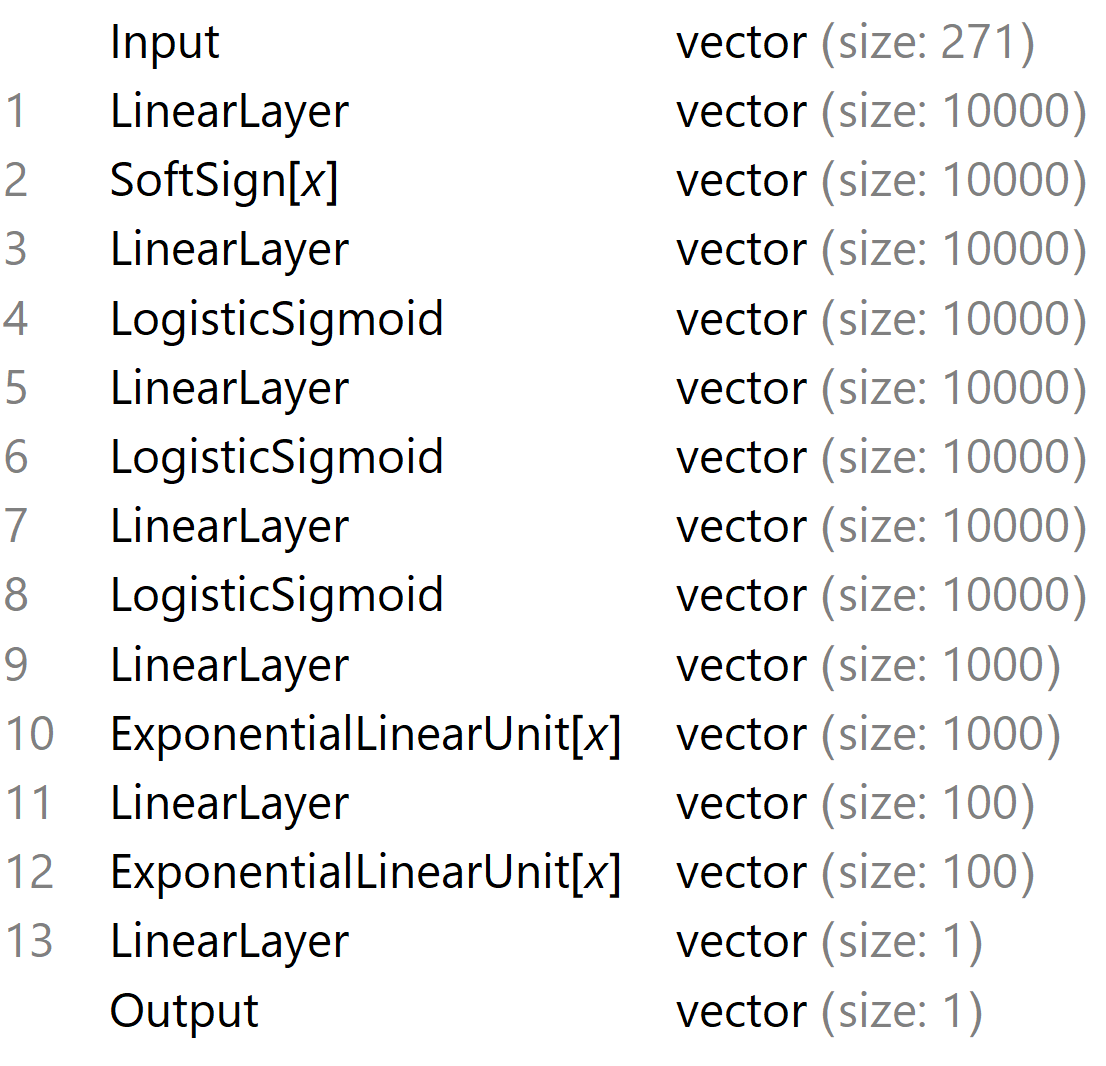
\includegraphics[width=0.30\textwidth]{sipfenn/NN9_architecture.PNG}}
    \hspace{6pt}
    \frame{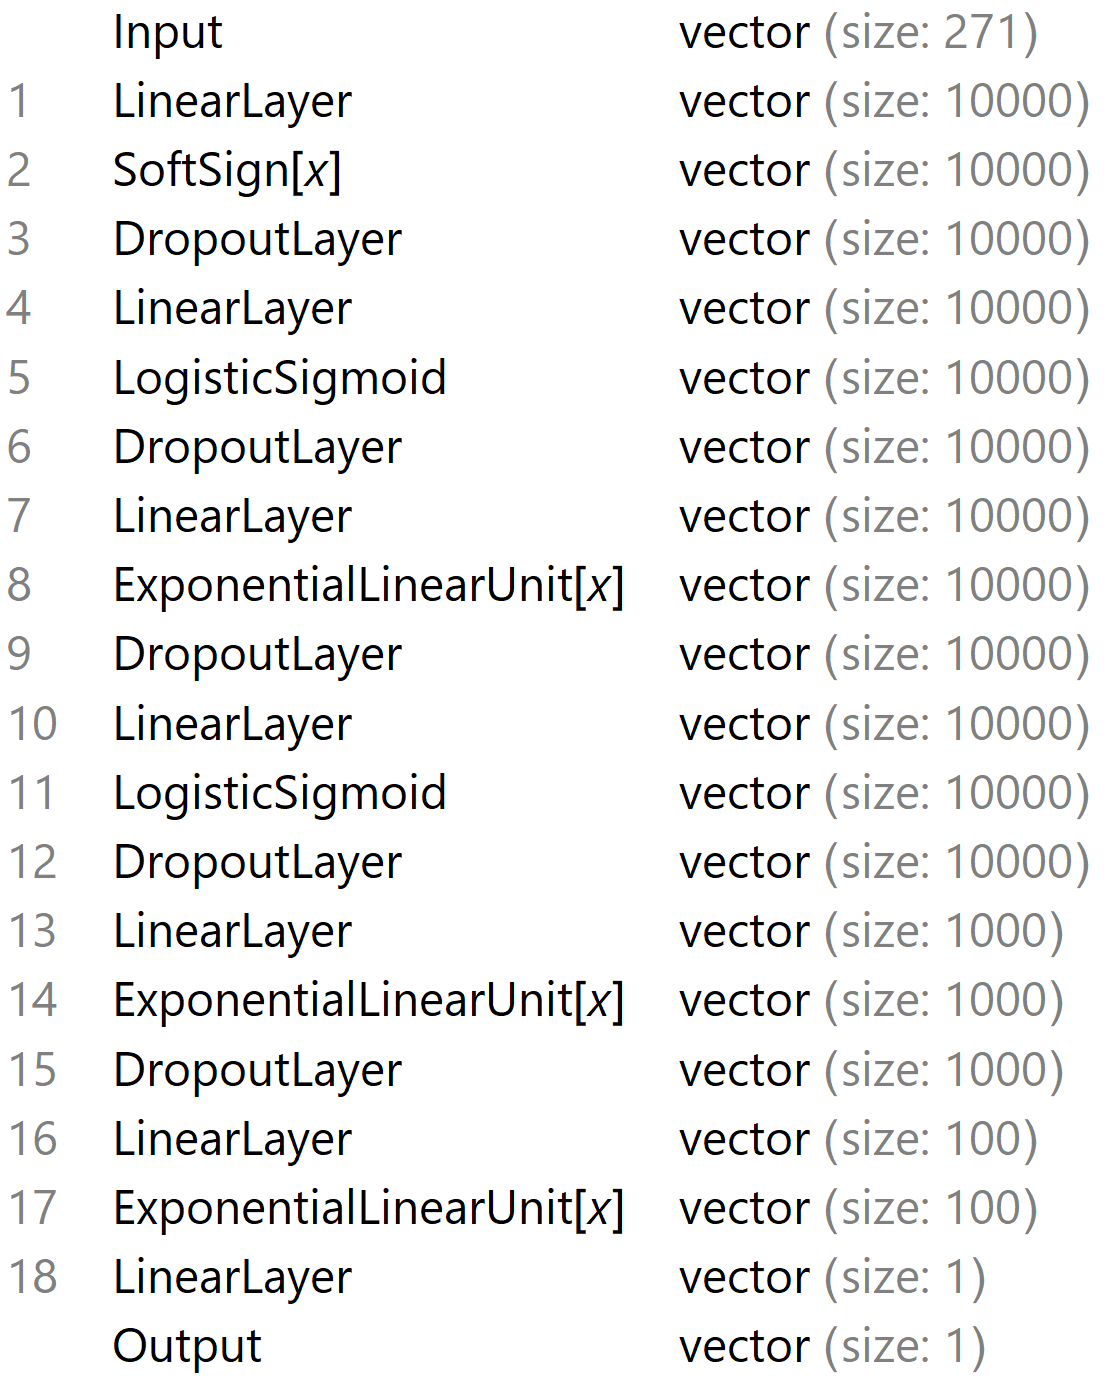
\includegraphics[width=0.30\textwidth]{sipfenn/NN20_architecture.PNG}}
    \hspace{6pt}
    \frame{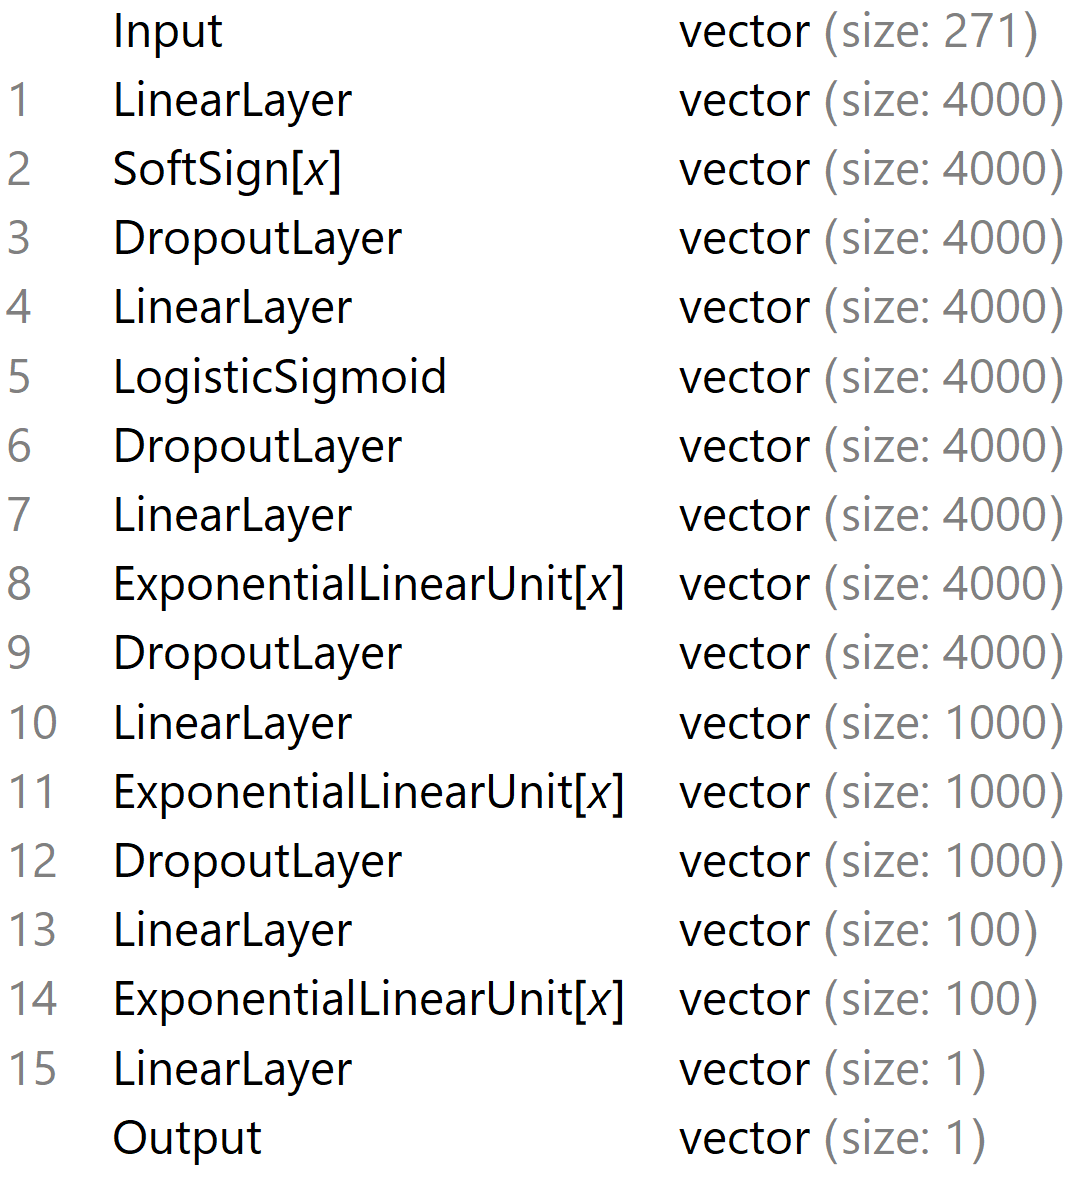
\includegraphics[width=0.30\textwidth]{sipfenn/NN24_architecture.PNG}}
    \caption{Three selected architectures designed within the present work. Optimized for: (Left) OQMD performance, (Middle) predicting new materials, (Right) small size at good performance. Internally in the code, they are designated as NN9, NN20, and NN24.}
    \label{sipfenn:fig:architectures}
\end{figure}

Out of all trained neural networks, three were selected and can be considered final outcomes of the design process, optimized for different objectives. Their architectures are presented in Figure \ref{sipfenn:fig:architectures}. The first one, denoted NN9, was created specifically for the OQMD performance. This was the same objective as in the study by Ward et al. \cite{Ward2017IncludingTessellations} and its performance serves as a direct comparison to the Random Forest method employed in that paper \cite{Ward2017IncludingTessellations} and other works \cite{Schutt2014HowProperties, Seko2017RepresentationProperties}.


\begin{figure}[H]
    \centering
    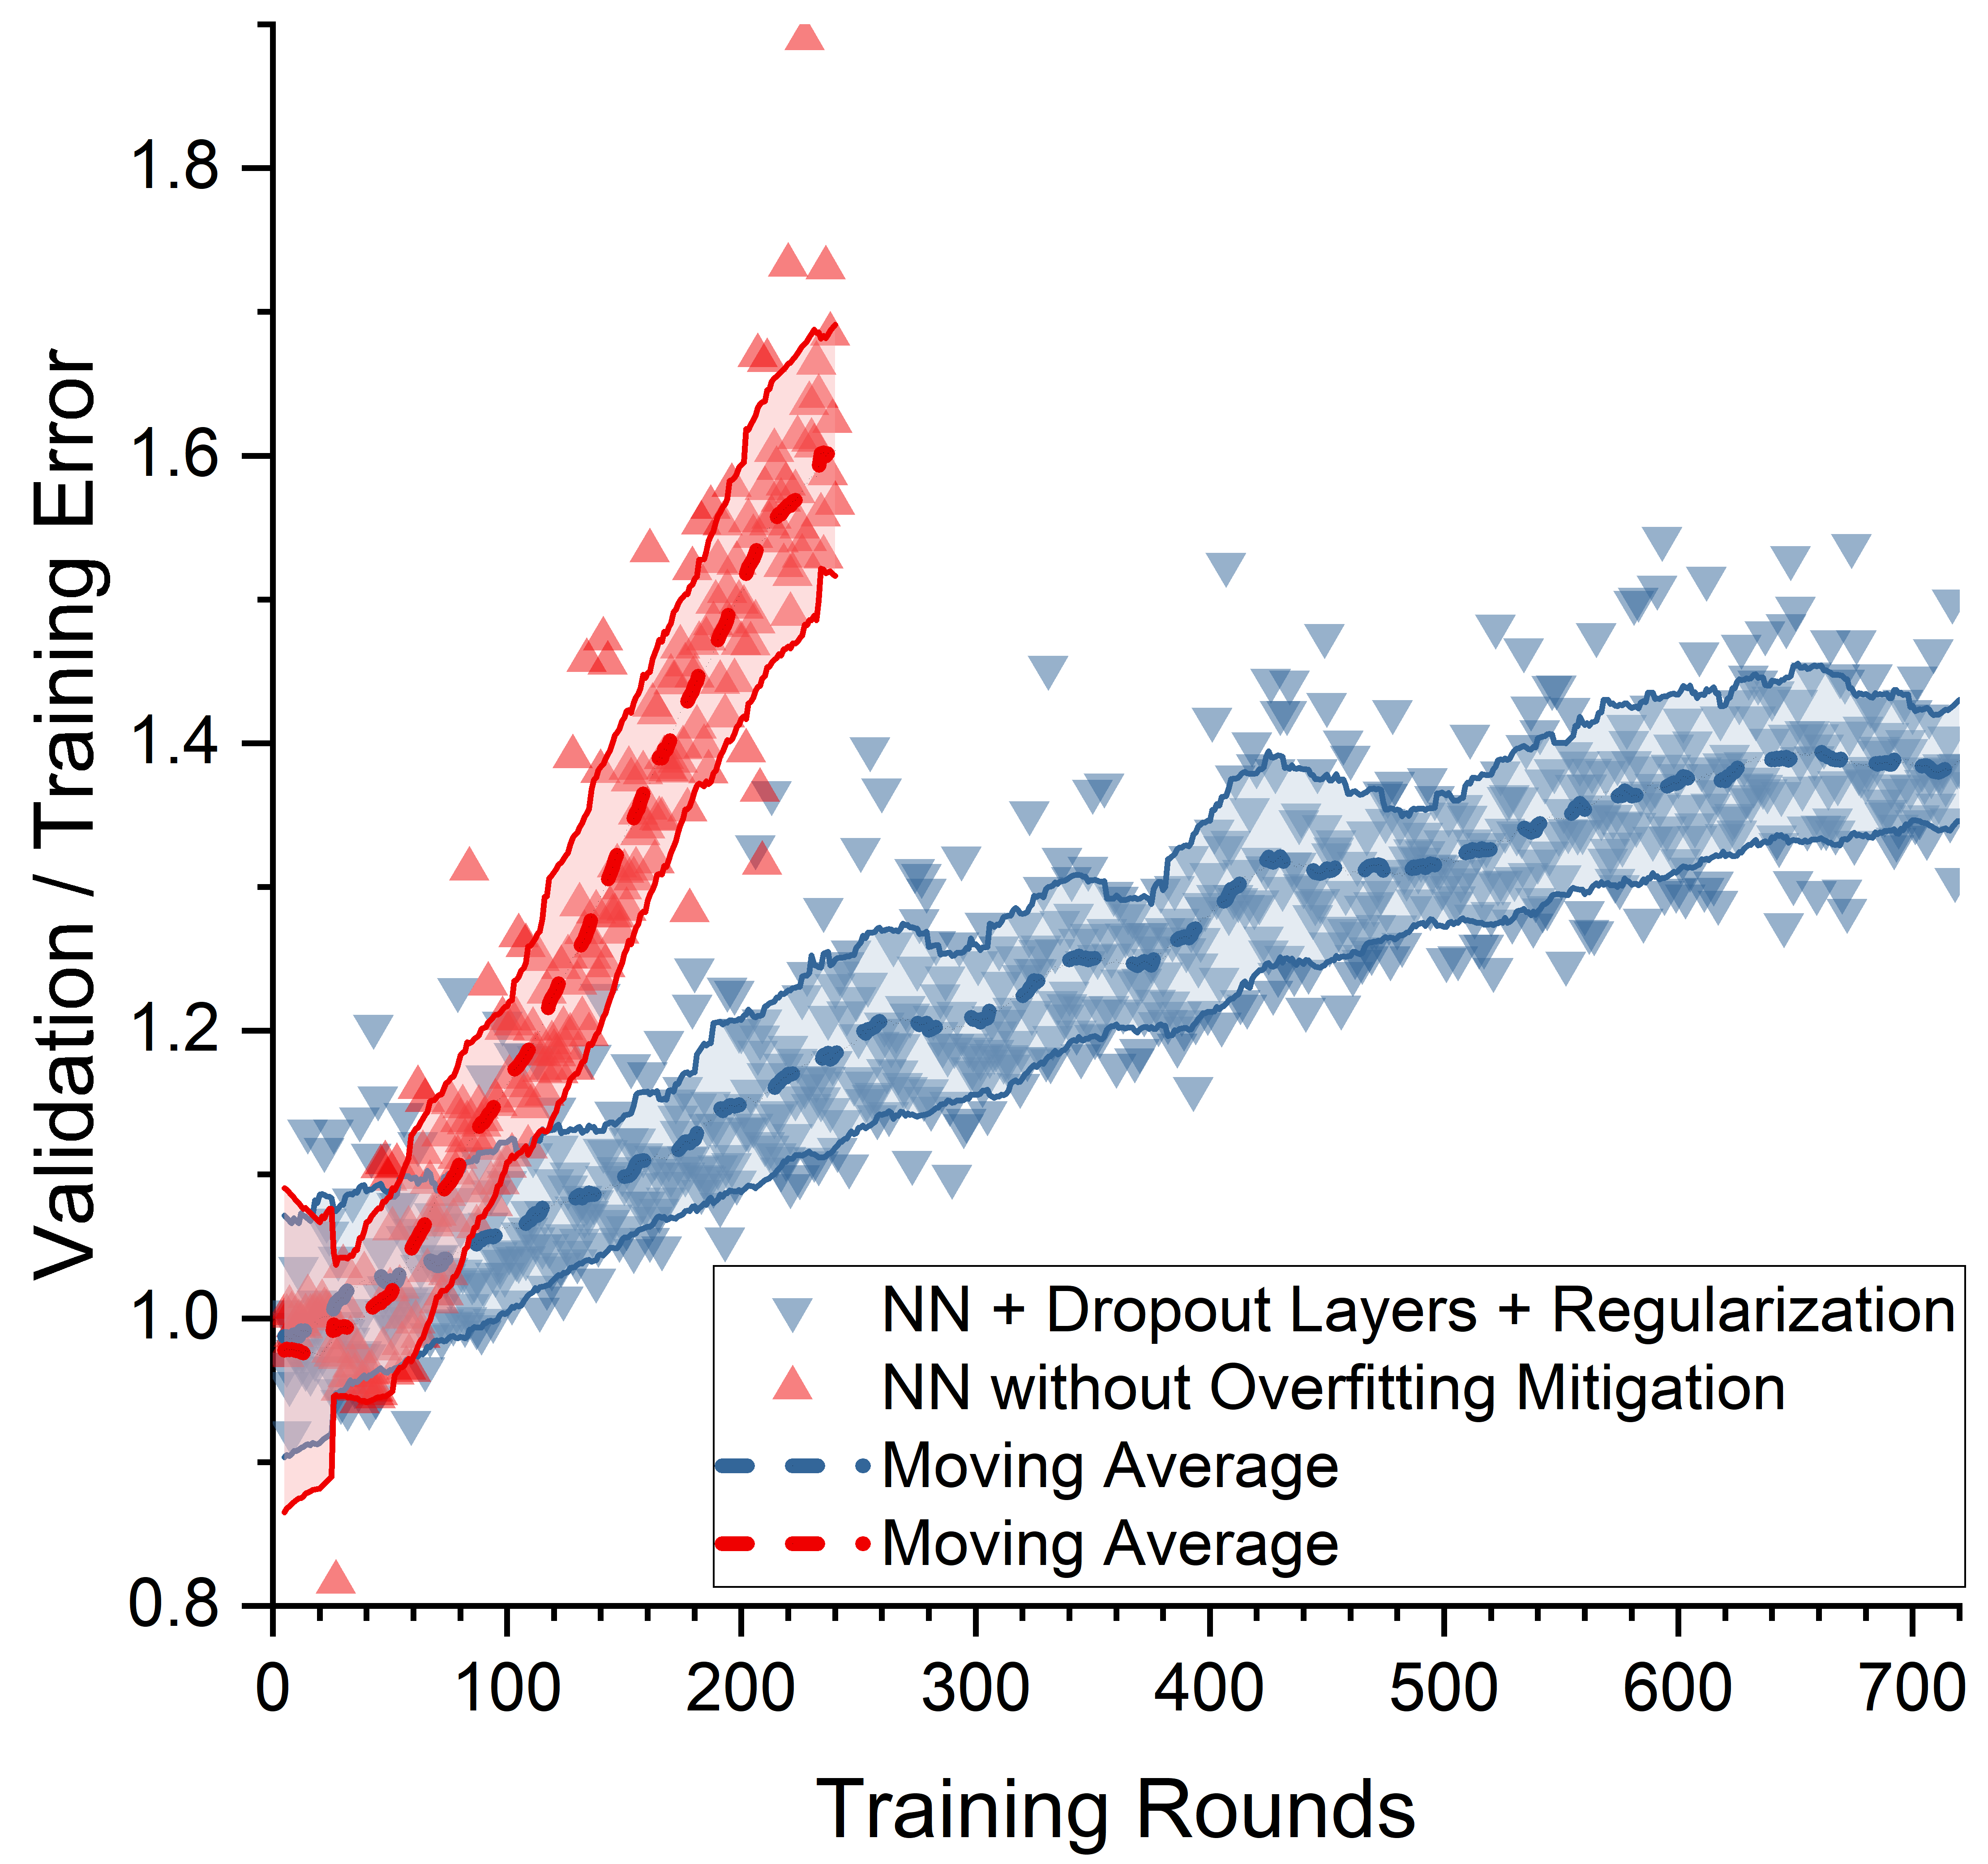
\includegraphics[width=0.52\textwidth]{sipfenn/validationtotraining_generalized.png}
    \caption{Training Loss to Validation Loss in a model that does without (NN9) and with overfitting mitigation (NN20), plotted versus training progress.}
    \label{sipfenn:fig:trainingvalidation-body}
\end{figure}

The second network was optimized for improved pattern recognition on OQMD and improved performance on non-OQMD datasets used in the present work (i.e. SQS/$\sigma$-phase datasets). This was achieved primarily through extensive overfitting mitigation, applied during design and training (see Figure \ref{sipfenn:fig:trainingvalidation-body}), which leads to a network with improved generalization/materials-discovery capability. Furthermore, one fo the overfitting mitigation methods, namely the regularization described in \ref{sipfenn:ref:machinelearningoverview}, have allowed identification of descriptor attributes that contributed the most to the predictive capability and the ones that were almost completely discarded once the penalty for considering them was assigned. Figure \ref{sipfenn:fig:squaredweights} presents the distribution of sums of squared weights between each neuron in the input layer (each of the 273 descriptor features) and all 10,000 neurons in the first hidden layer. 

\begin{figure}[h]
    \centering
    \begin{minipage}[c]{0.65\textwidth}
    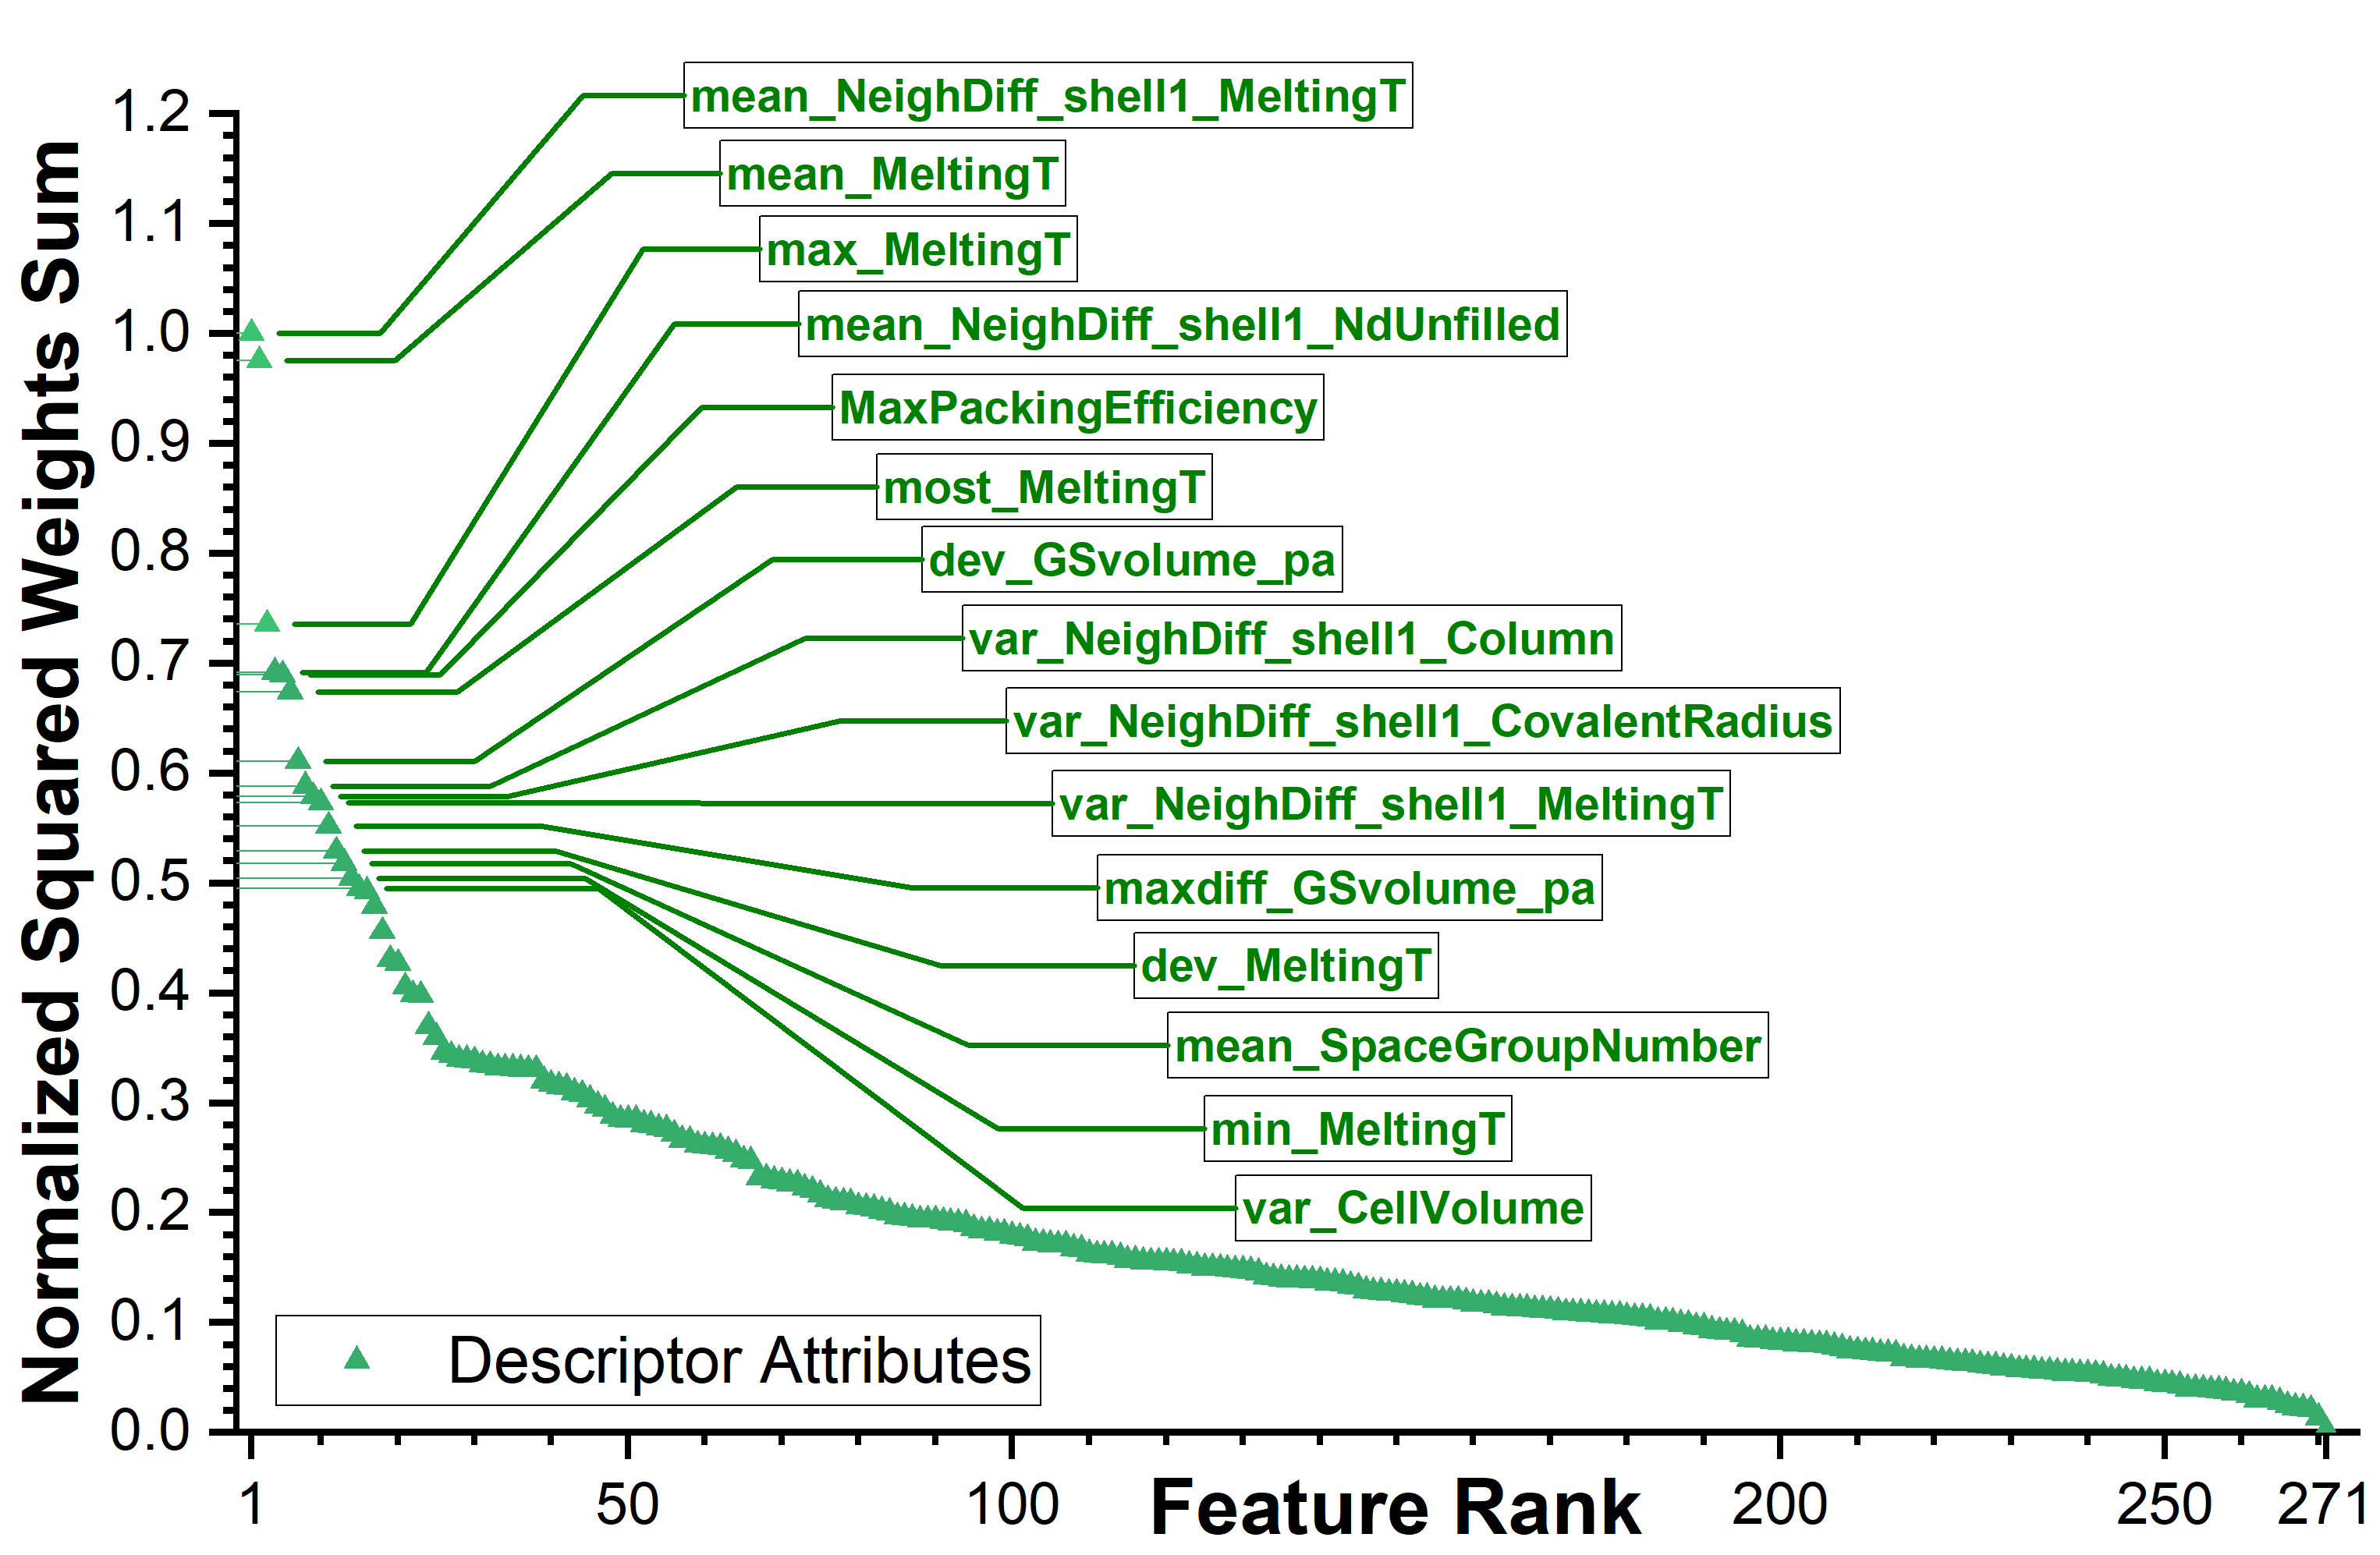
\includegraphics[width=\textwidth]{sipfenn/squaredweightssumNN20_V2.png}
    \end{minipage}\hfill
    \begin{minipage}[c]{0.33\textwidth}
    \caption{Distribution of sums of squared input weights. High values correspond to attributes that were not lowered due to their contribution to pattern recognition of the model. 15 attributes with the highest values are labeled. The labels are taken from the descriptor definition in  \cite{Ward2016AMaterials}.}
    \label{sipfenn:fig:squaredweights}
    \end{minipage}
\end{figure}

Feature rankings, such as presented in Figure \ref{sipfenn:fig:squaredweights}, allow a more efficient selection of input features in future studies looking into the same problem; thus both reducing the number of features that need to be computed for each atomic configuration and the total number of weights in the network. Furthermore, it can be used to gain an insight into the model interpretability. Looking at the specific ranking for NN20, the high-impact features present a mix of elemental features, likely allowing the model to establish some formation energy baseline for a given composition, and structure-informed features allowing to distinguish between polymorphic configurations. High impact elemental features include different statistics on elemental melting temperatures and ground-state structure volume per atom. The structural features extend them by considering how they differ between neighboring atoms and also include purely structural features such as packing efficiency and variance in Wigner–Seitz cells volumes. A complete ranking of features is included in Appendix \ref{sipfenn:appendix3}.

The third network, denoted NN24, was created for memory/power-constrained applications requiring a balance between OQMD performance and memory intensity and processing power required. Model parameters contained in this architecture occupy only 145MB, over 8 times less than two other models and around 200 times less than the model reported by Ward et al. \cite{Ward2017IncludingTessellations}.

\subsection{OQMD Data Performance} \label{sipfenn:ssec:oqmdperformance}
As described in \ref{sipfenn:sssec:NetDesign}, all three final networks were evaluated on a randomly selected subset of the OQMD to give a comparison between the state-of-the-art model presented by Ward et al. \cite{Ward2017IncludingTessellations} and the present ML method. This random subset consisted of 21,800 OQMD entries, constituting approximately $5\%$, which were not presented to the network, nor used for evaluation at any stage of the training process. This sample size was considered to be representative of the whole dataset once the small fraction ($0.026\%$) of likely incorrect entries were removed from the dataset as described in \ref{sipfenn:sssec:Data}. The random selection itself was initially performed separately for each training process and recorded after completion. Later, when networks were modified to mitigate overfitting, a single random subset was used for all of them to allow more careful design and more accurate comparative analysis of results. Figure \ref{sipfenn:fig:oqmdperformance} gives (1) prediction vs OQMD values of formation energy plot, (2) statistics related to the error in predictions relative to the OQMD values, and (3) a histogram of the absolute error in predictions relative to the OQMD values.

\begin{figure}[H]
    \centering
    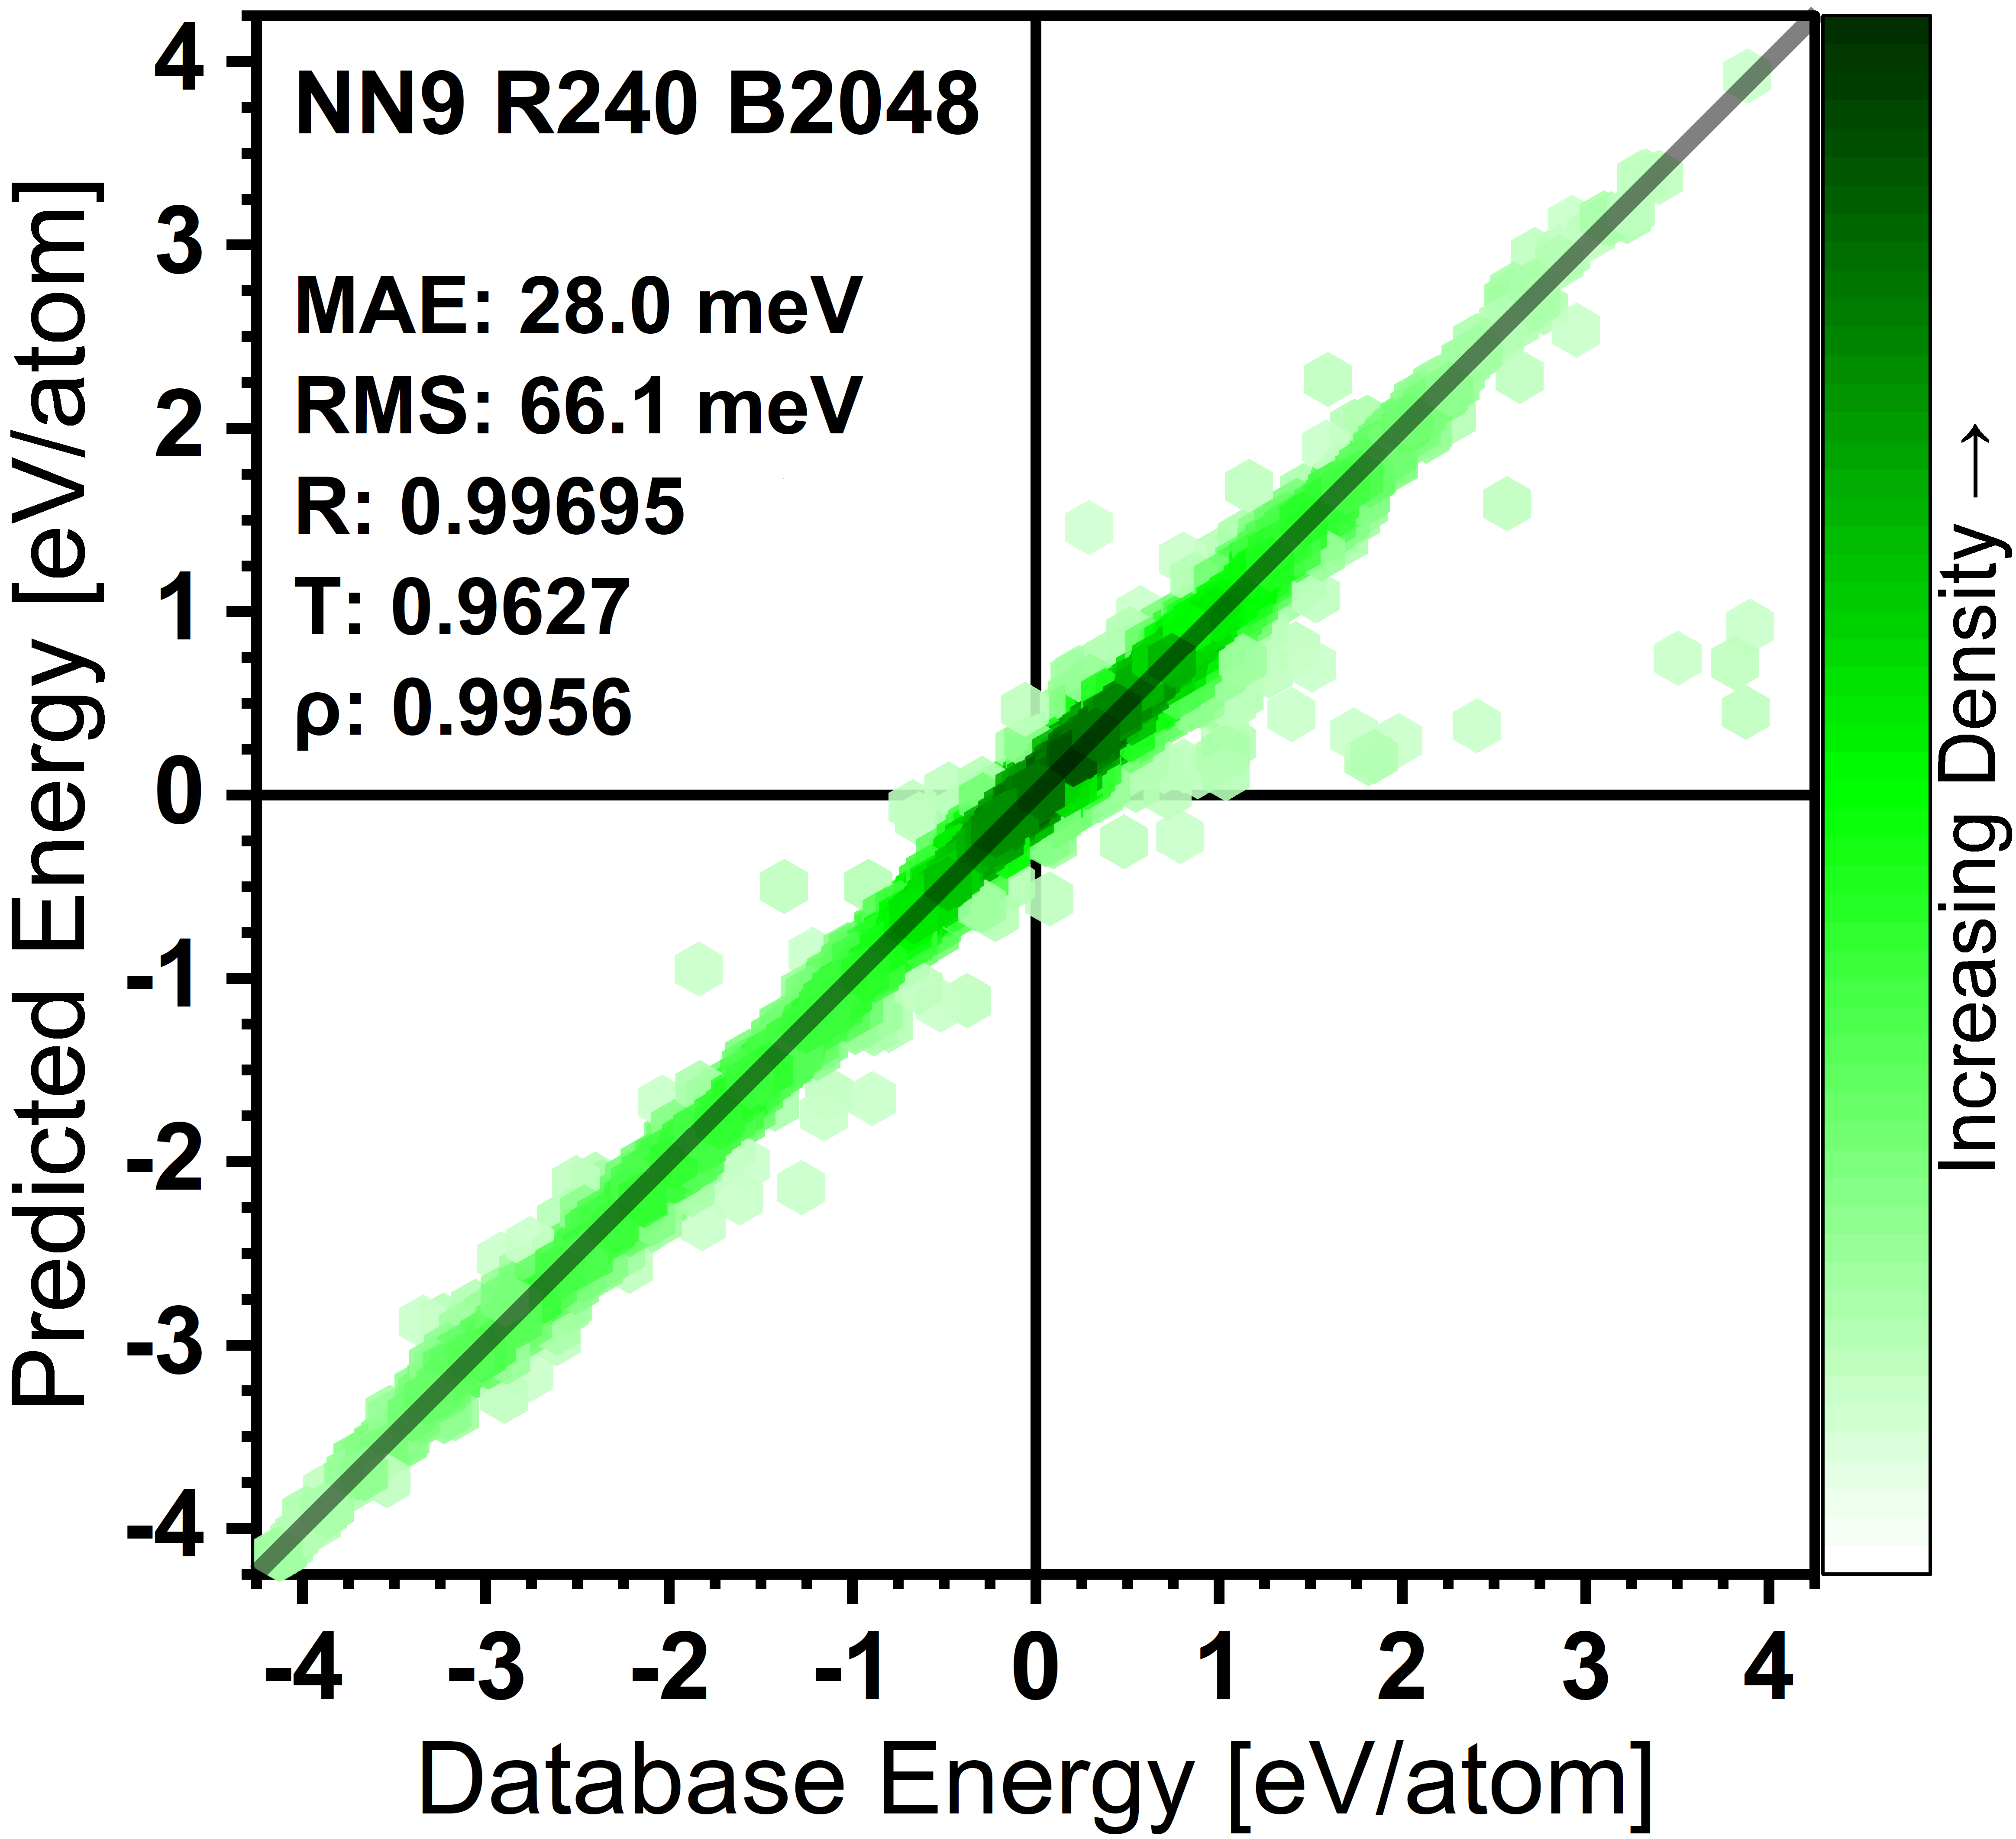
\includegraphics[width=0.31\textwidth]{sipfenn/NN9_test.png}
    \hspace{0.01\textwidth}
    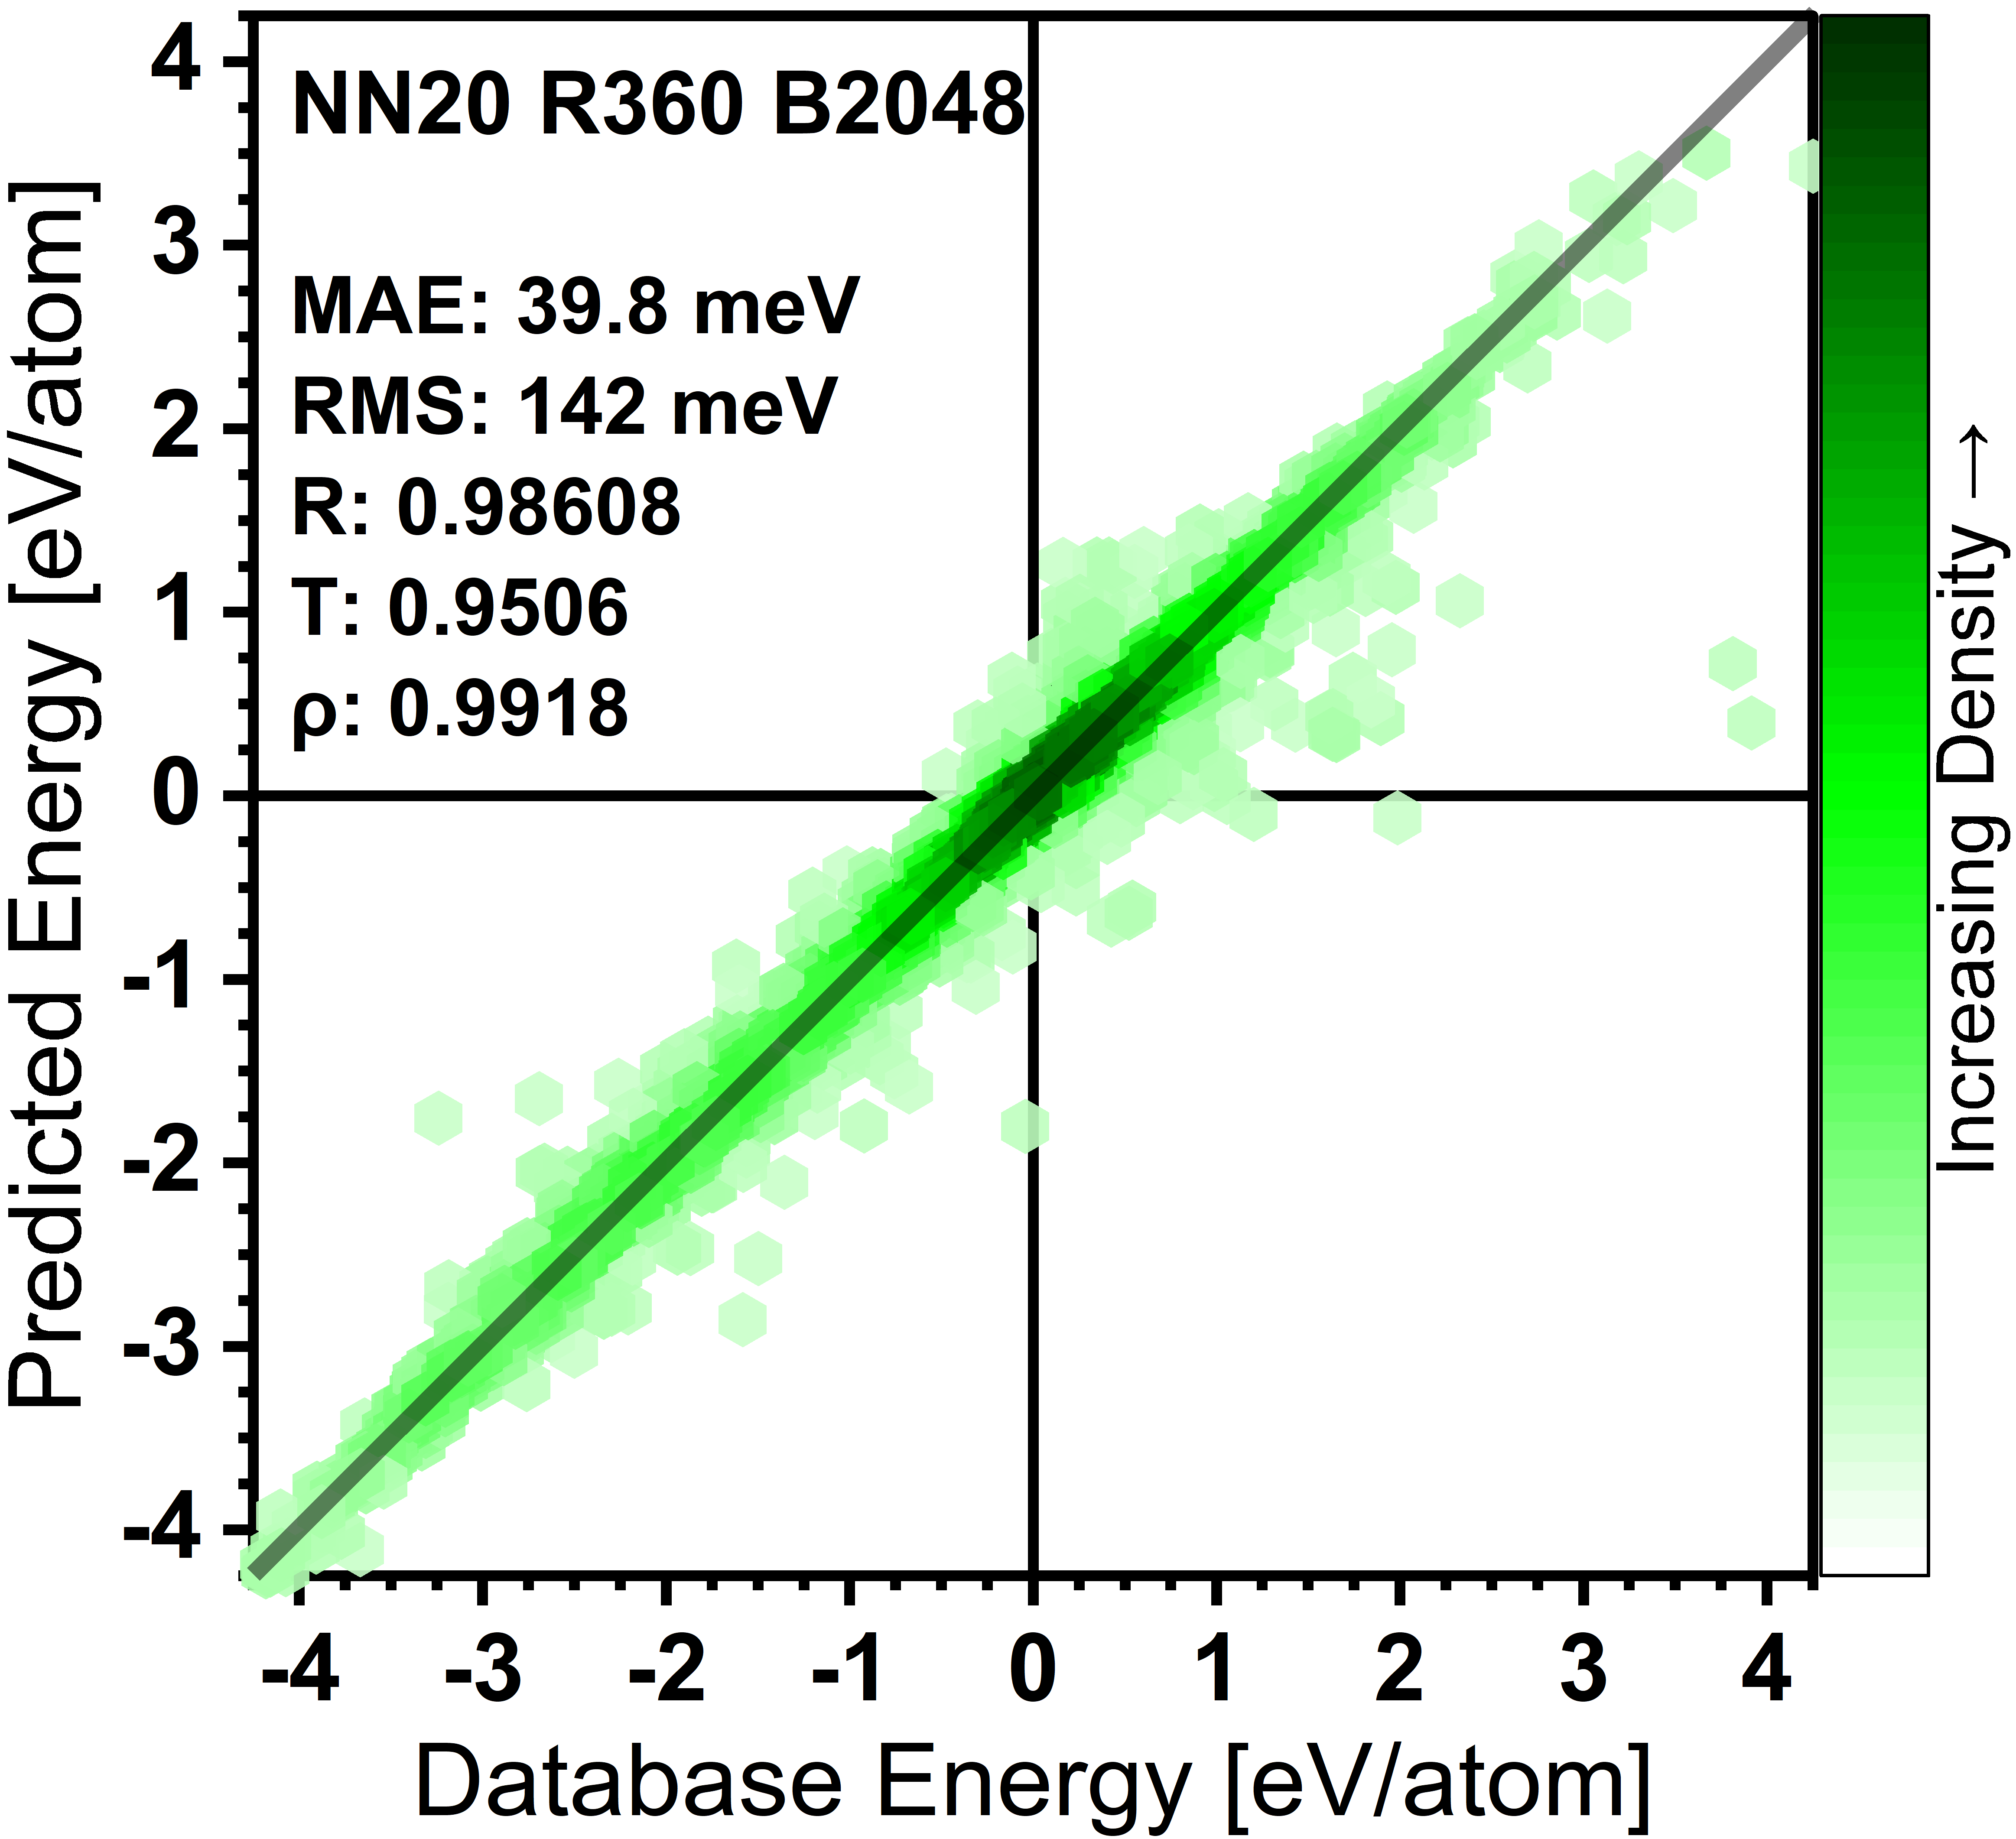
\includegraphics[width=0.31\textwidth]{sipfenn/NN20_test.png}
    \hspace{0.01\textwidth}
    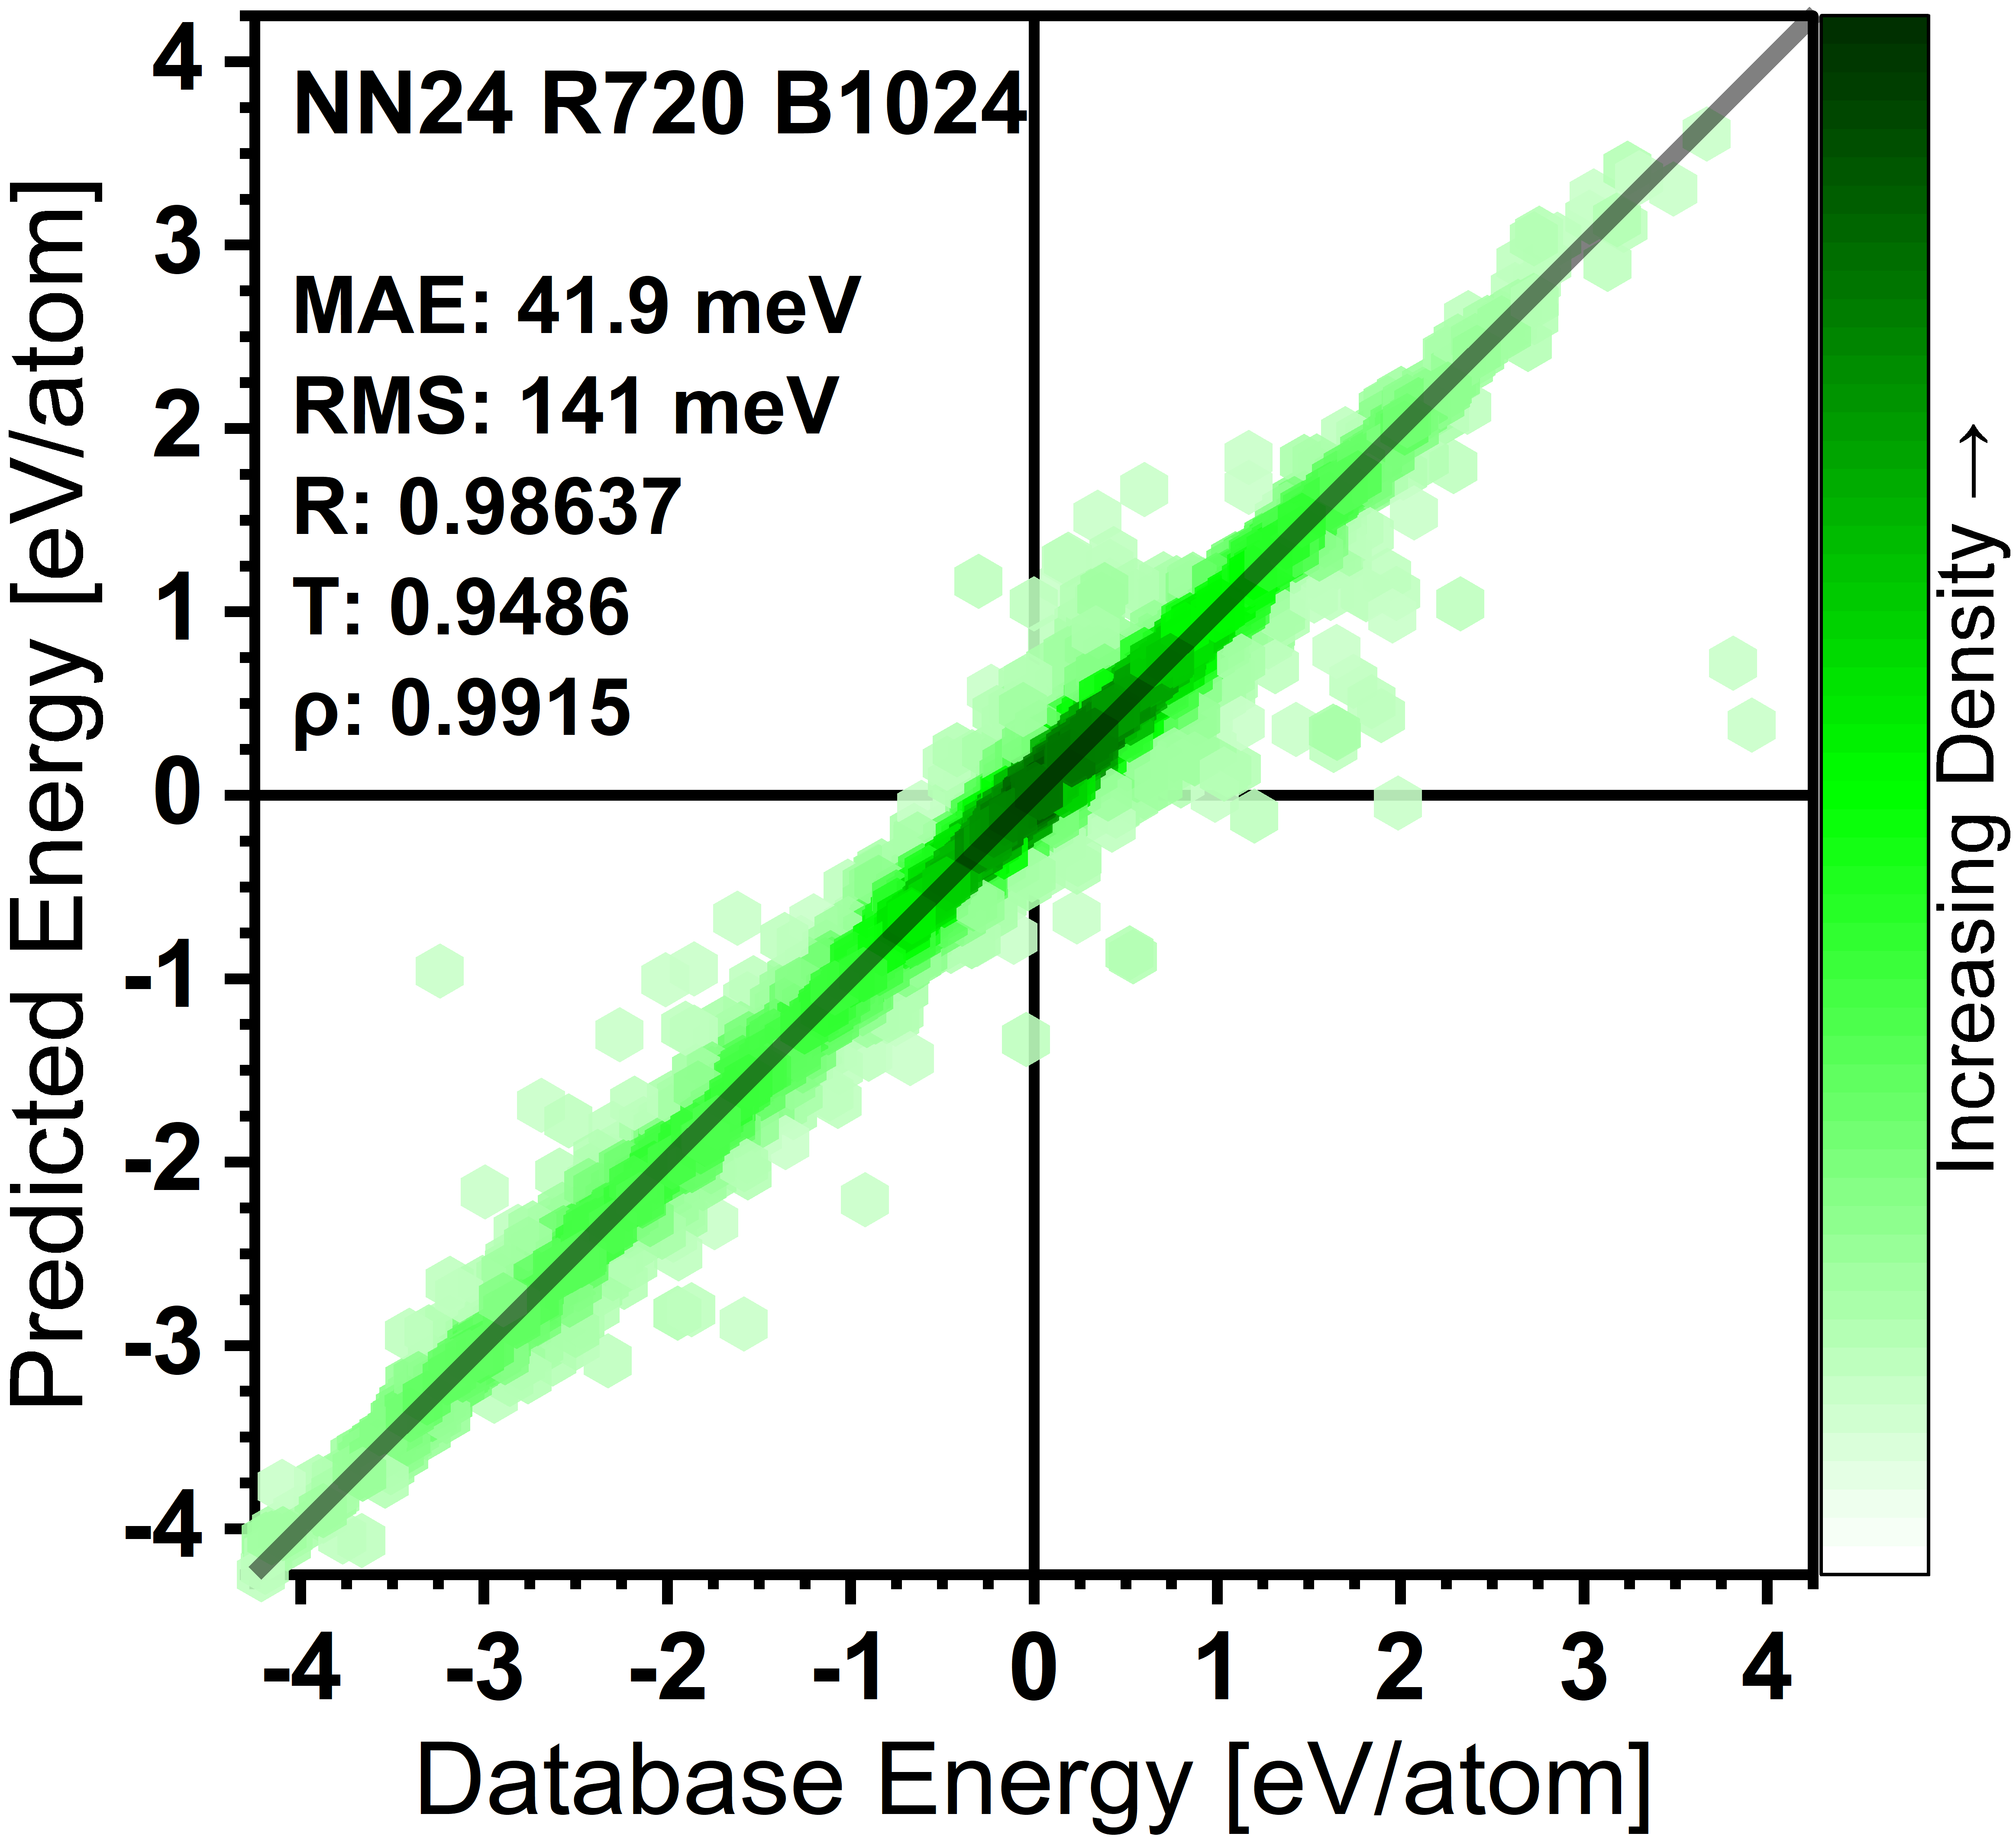
\includegraphics[width=0.31\textwidth]{sipfenn/NN24_test.png}
    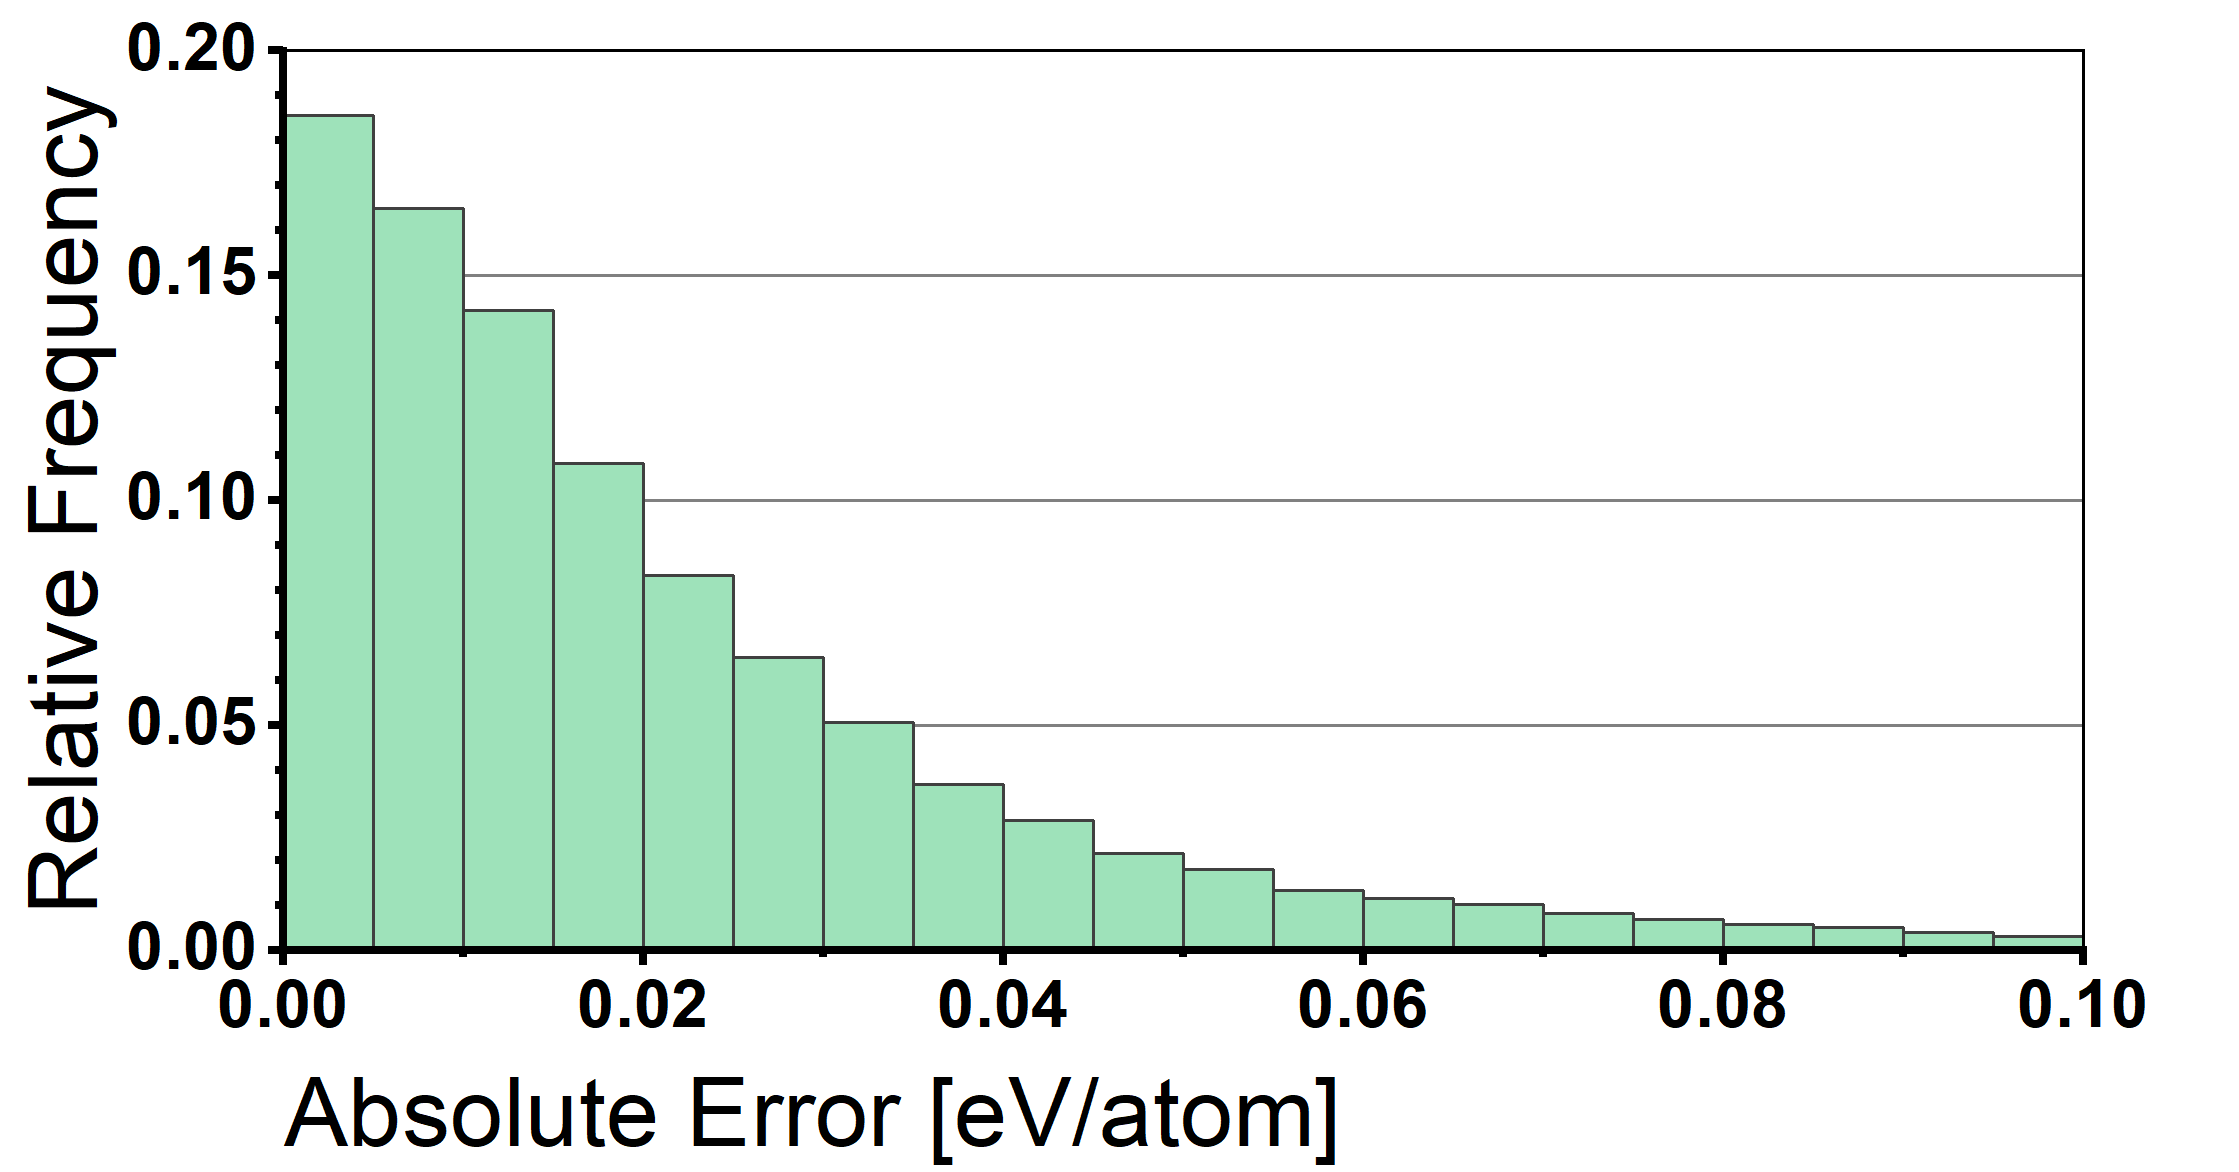
\includegraphics[width=0.31\textwidth]{sipfenn/nn9_histogram.png}
    \hspace{0.01\textwidth}
    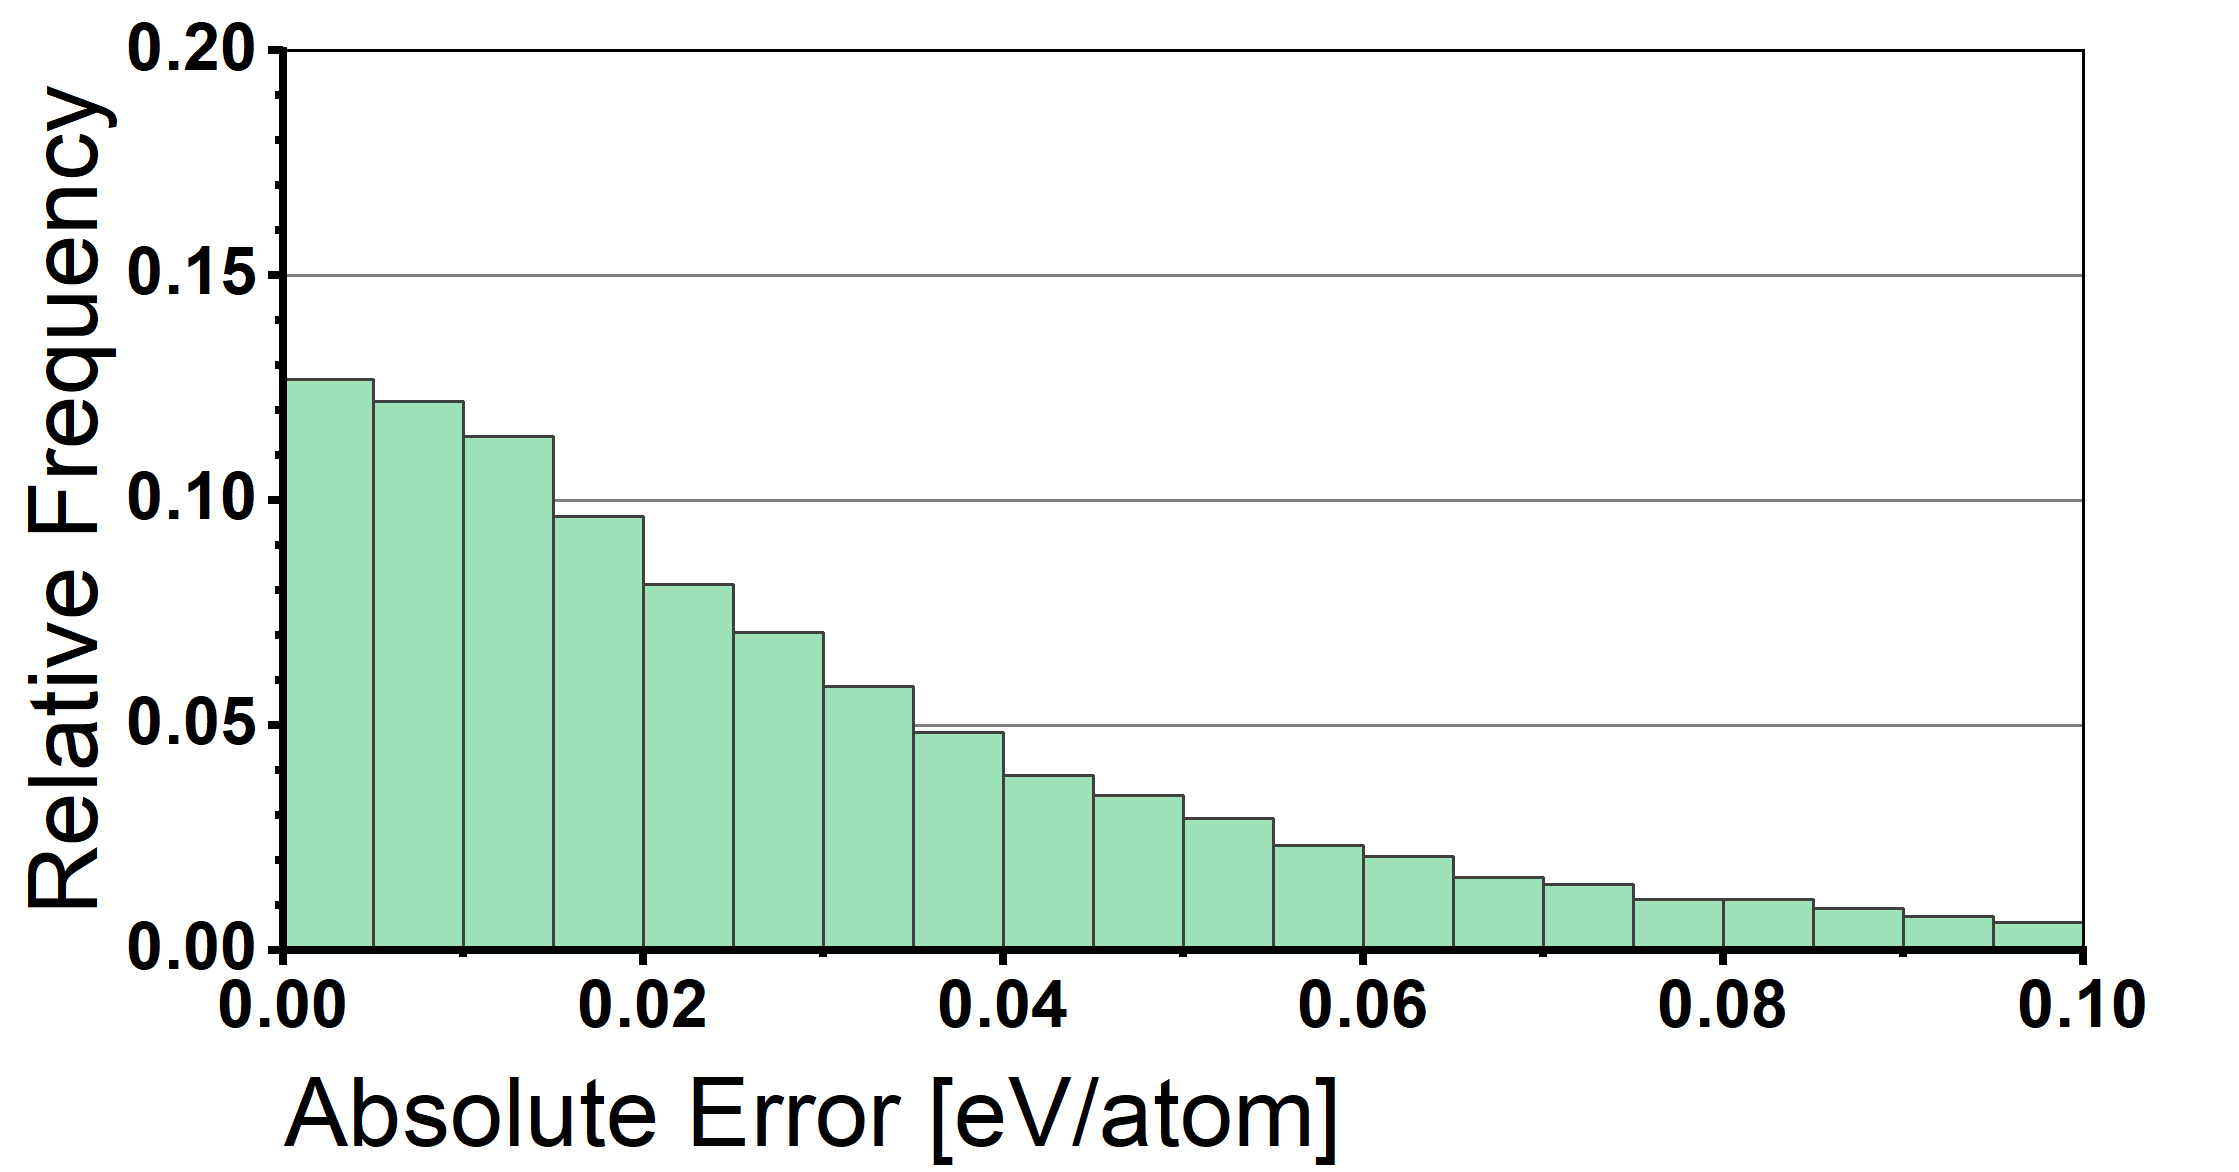
\includegraphics[width=0.31\textwidth]{sipfenn/nn20_histogram.png}
    \hspace{0.01\textwidth}
    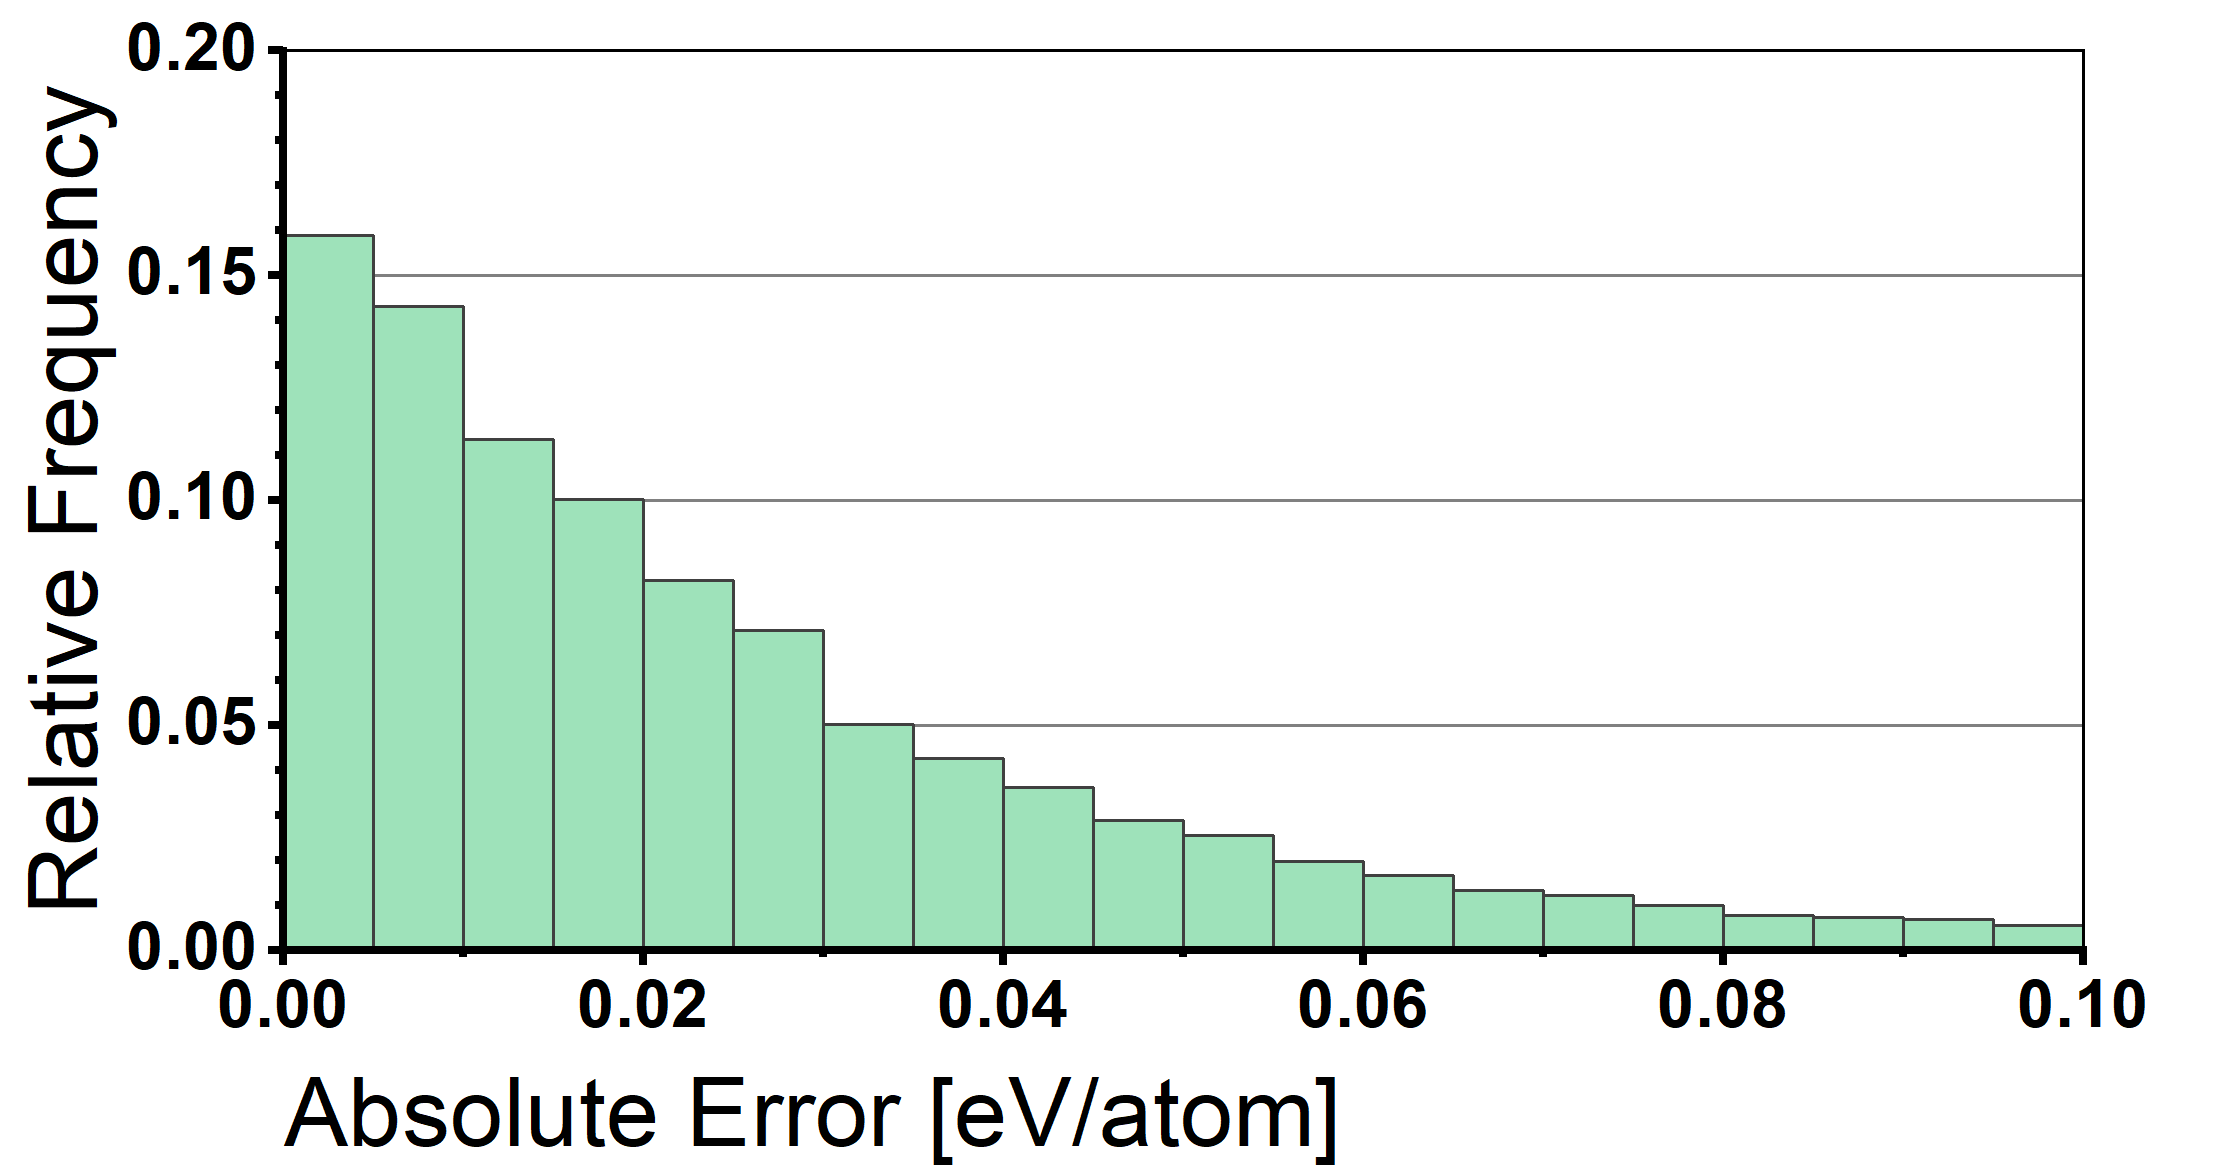
\includegraphics[width=0.31\textwidth]{sipfenn/nn24_histogram.png}
    \caption{Performance of 3 selected neural networks on a random subset of 21,800 entries from OQMD. (Left) OQMD performance, (Middle) predicting new materials, (Right) small size at good performance. Internally in the code, they are designated as NN9, NN20, and NN24.}
    \label{sipfenn:fig:oqmdperformance}
\end{figure}

\subsection{Existing Methods Comparison} \label{sipfenn:ssec:existing}
In this section, the performance of the models is compared with a few similar existing approaches based on the OQMD dataset, when formation energy of a structure is predicted \cite{Ward2016AMaterials, Ward2017IncludingTessellations, Jha2019IRNet}, or its subset of the convex-hull structures, when formation energy of the most stable structure is predicted \cite{Jha2018ElemNet:Composition, Goodall2020PredictingStoichiometry}.  This division is made based on the reasoning presented in \ref{sipfenn:ssec:currentapproach}. While the latter type cannot be used to predict the formation energy of any arbitrary structure, the structure-informed models like \texttt{SIPFENN} (the present work) can be tested on the convex hull structures. 


\begin{table}[H]
\begin{center}
\begin{tabular}{|c|c|c|}
\hline
 Method & Formation Energy MAE & Convex Hull MAE \\
 \hline
 \texttt{SIPFENN} (This Work) & \textbf{28.0 meV/atom} (OQMD Opt.) & 32meV/atom (Novel. Mat.) \\
 \texttt{Ward2017} \cite{Ward2016AMaterials, Ward2017IncludingTessellations} & 80 meV/at & N/M \\
 \texttt{ElemNet} \cite{Jha2018ElemNet:Composition} & N/A & 50 meV/at\\  
 \texttt{IRNet} \cite{Jha2019IRNet} & 38 meV & N/M \\
 \texttt{Roost} \cite{Goodall2020PredictingStoichiometry} & N/A & 29 meV/at | \textbf{24 meV/at}\\
 \hline
\end{tabular}
\caption{Comparison of our method with existing state-of-the-art methods, as of late 2020, with OQMD-optimized \texttt{SIPFENN} model exhibiting state-of-the-art performance. N/A and N/M respectively stand for not applicable (out of domain) and not measured.}
\label{sipfenn:comparison-results}
\end{center}
\vspace{-24pt}
\end{table}

The results are shown in Table \ref{sipfenn:comparison-results}. The \texttt{SIPFENN} convex hull MAE has been reported based on using the Novel Materials Model limiting the original test set to structures laying within 50meV/atom from the convex hull. From these results, we can see that the \texttt{SIPFENN} neural networks approach outperforms existing state-of-the-art methods for predicting the formation energy of any material. At the same time, while not being the best, it is capable of reaching performance levels of specialized models in predicting the formation energies of structures laying on the convex hull.

\subsection{Non-OQMD Data Performance} \label{sipfenn:ssec:sigmasqsperformance}

%\begin{figure}[H]
%    \centering
%    %\vspace{-48pt}
%    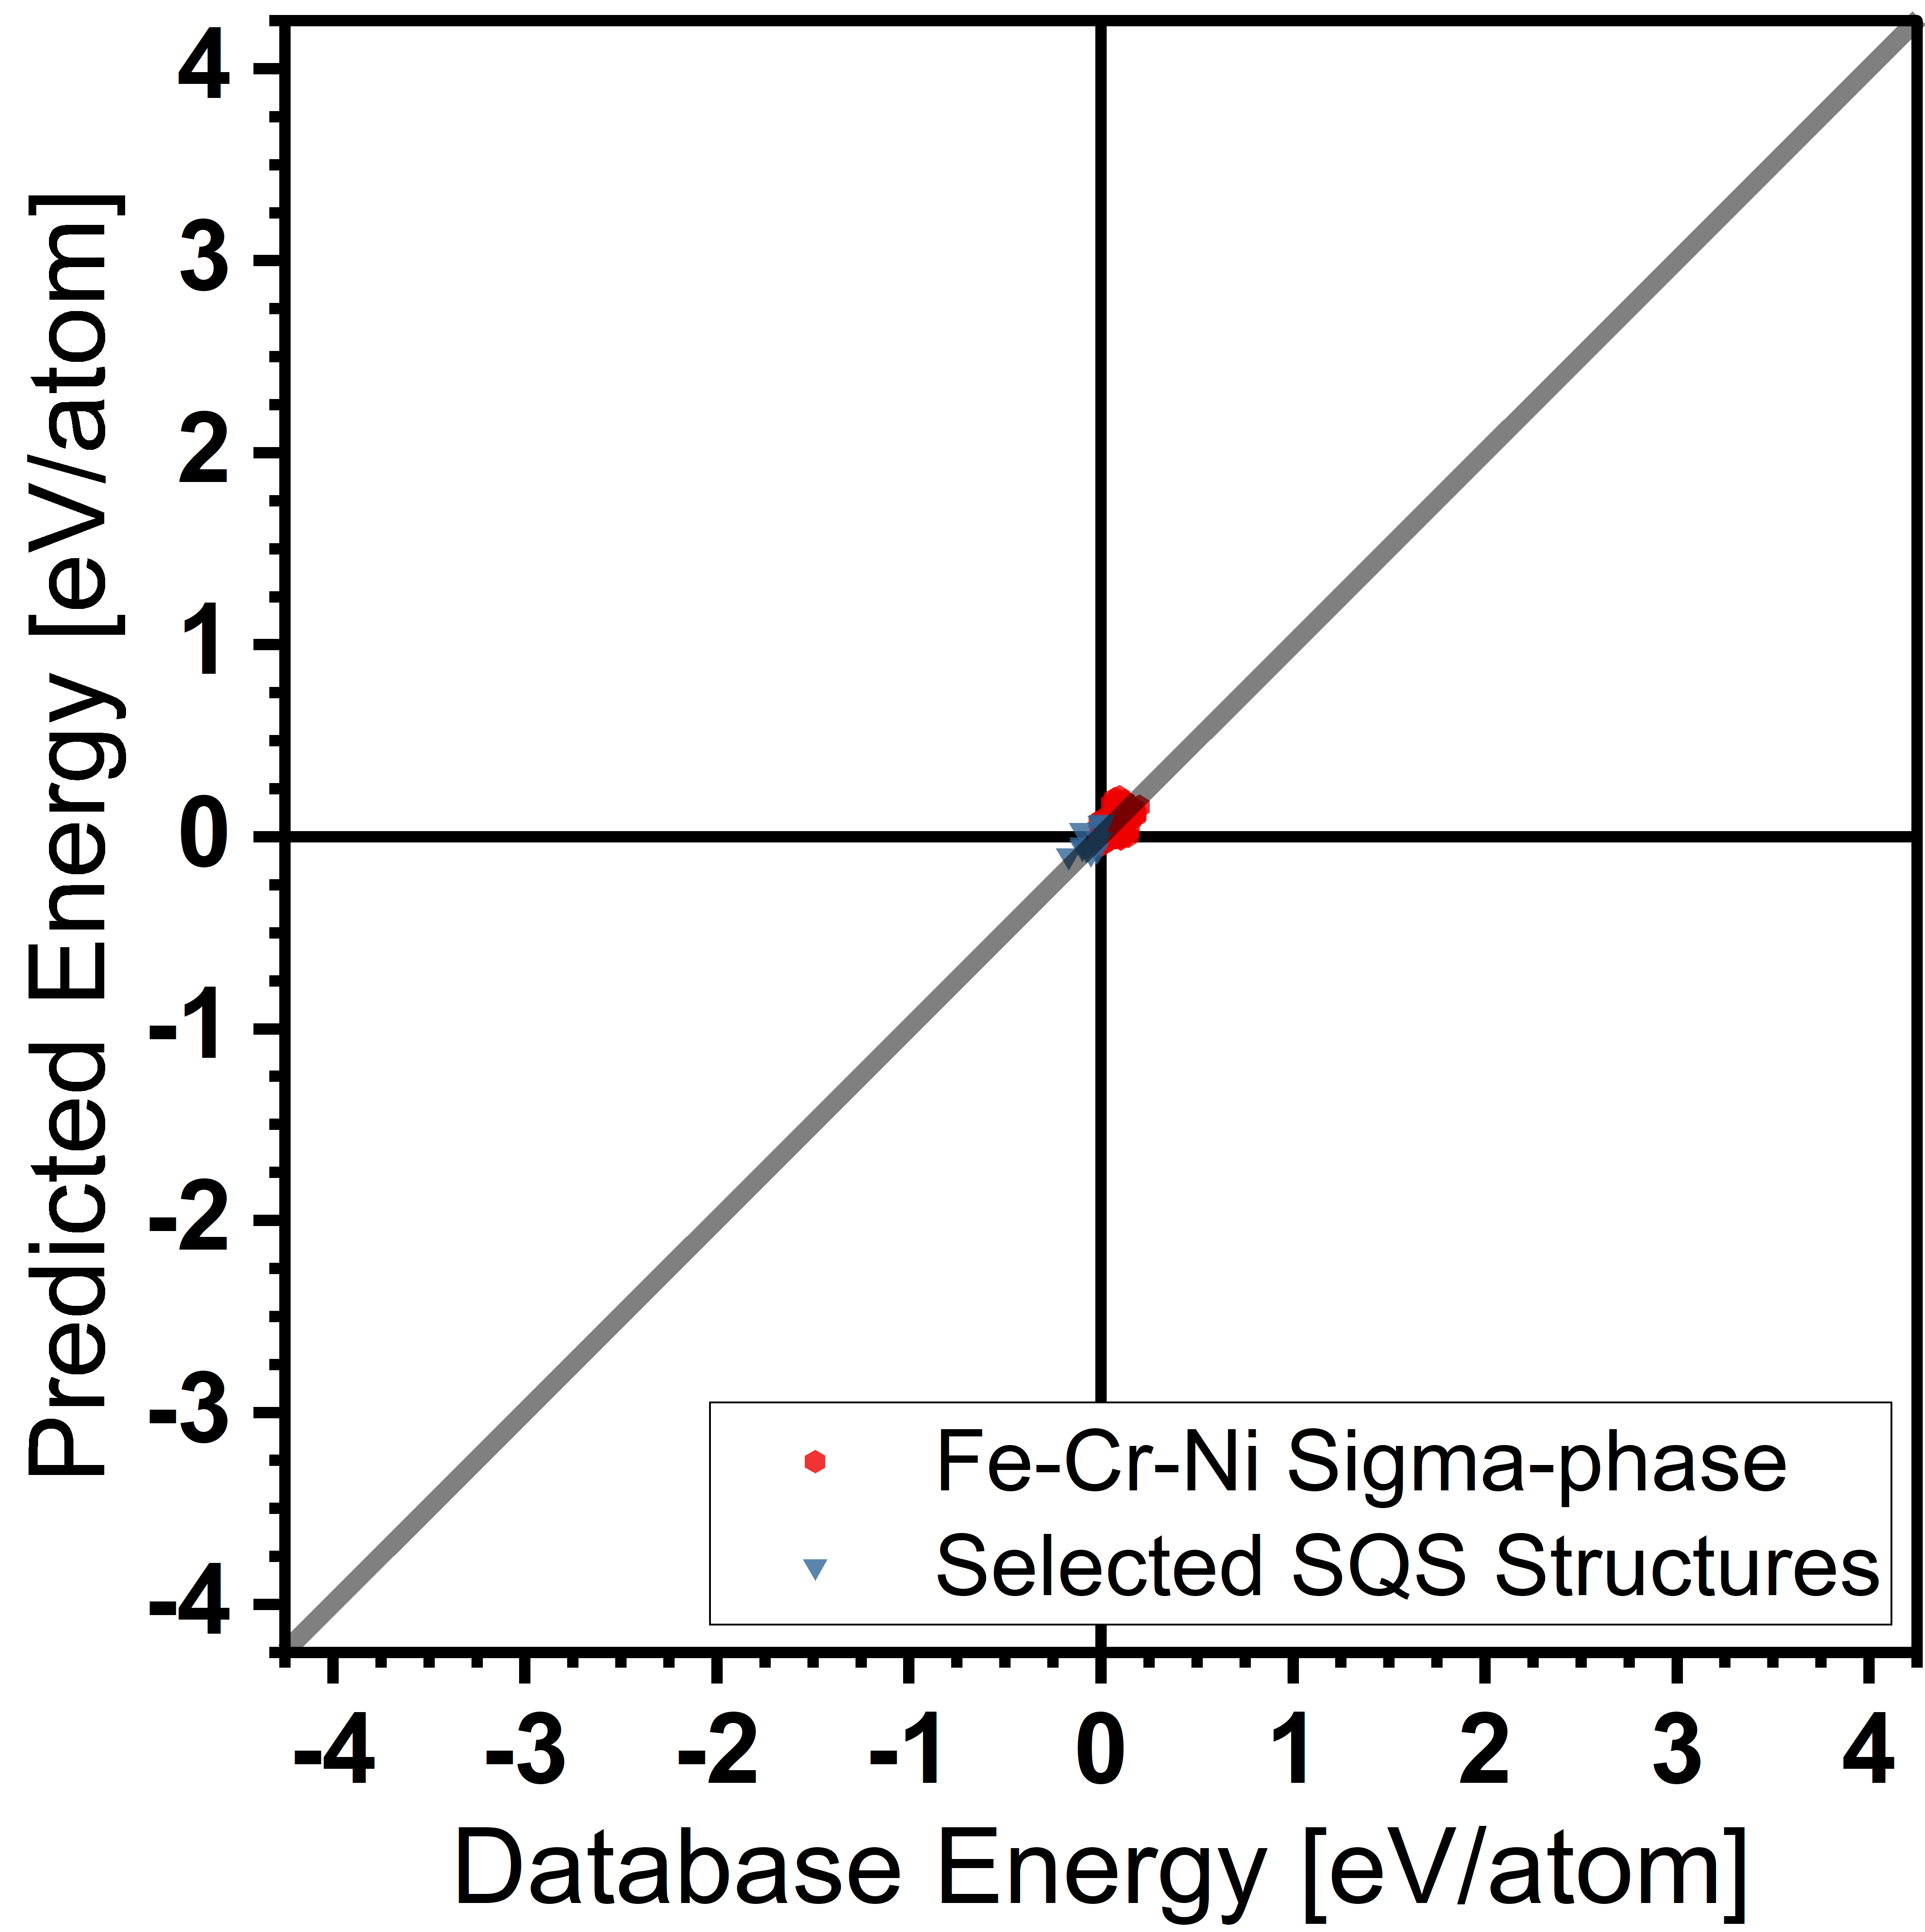
\includegraphics[width=0.3\textwidth]{sipfenn/NN20_test_sigmasqs.png}
%    \caption{Predictions of formation energy using the new-materials-optimized network (NN20) evaluated on (red) Fe-Cr-Ni $\sigma$-phase, and (blue) SQS structures. Compare to Figure \ref{sipfenn:fig:oqmdperformance} with the same axis for OQMD data.}
%    \label{sipfenn:fig:sqssigmabroad}
%    \vspace{-12pt}
%\end{figure}

Models created in the present work, specifically the ones optimized for predicting the formation energy of new materials, were designed and implemented to serve as tools for materials discovery. Evaluating their performance on data from the same source as the training set done in \ref{sipfenn:ssec:oqmdperformance} is inherently biased towards favoring models that provide the best fit to the prior (training) knowledge. This is amplified by the fact that many entries in the database are reported in groups that come from common studies and span similar materials, causing high domain clustering, which in some cases effectively makes such evaluation more akin to interpolation than extrapolation of knowledge.

To partially mitigate the described issue, the performance of the models was also evaluated on two smaller non-OQMD databases, described in \ref{sipfenn:sssec:Data}, representing an example of chemistries and structures that were of interest to the authors project on Ni-based superalloys. At the same time, they were not directly presented to the network in any capacity during the training process.

In all cases, models created in the present paper were able to achieve approximately the same performance as on a random selection from the OQMD. To give a more in-depth analysis of the results, Figure \ref{sipfenn:fig:sigmasqsperformance} shows a magnified view of the predictions and basic statistics on the agreement between predictions and the database for the three models developed in the present work.

\begin{figure}[H]
\centering
    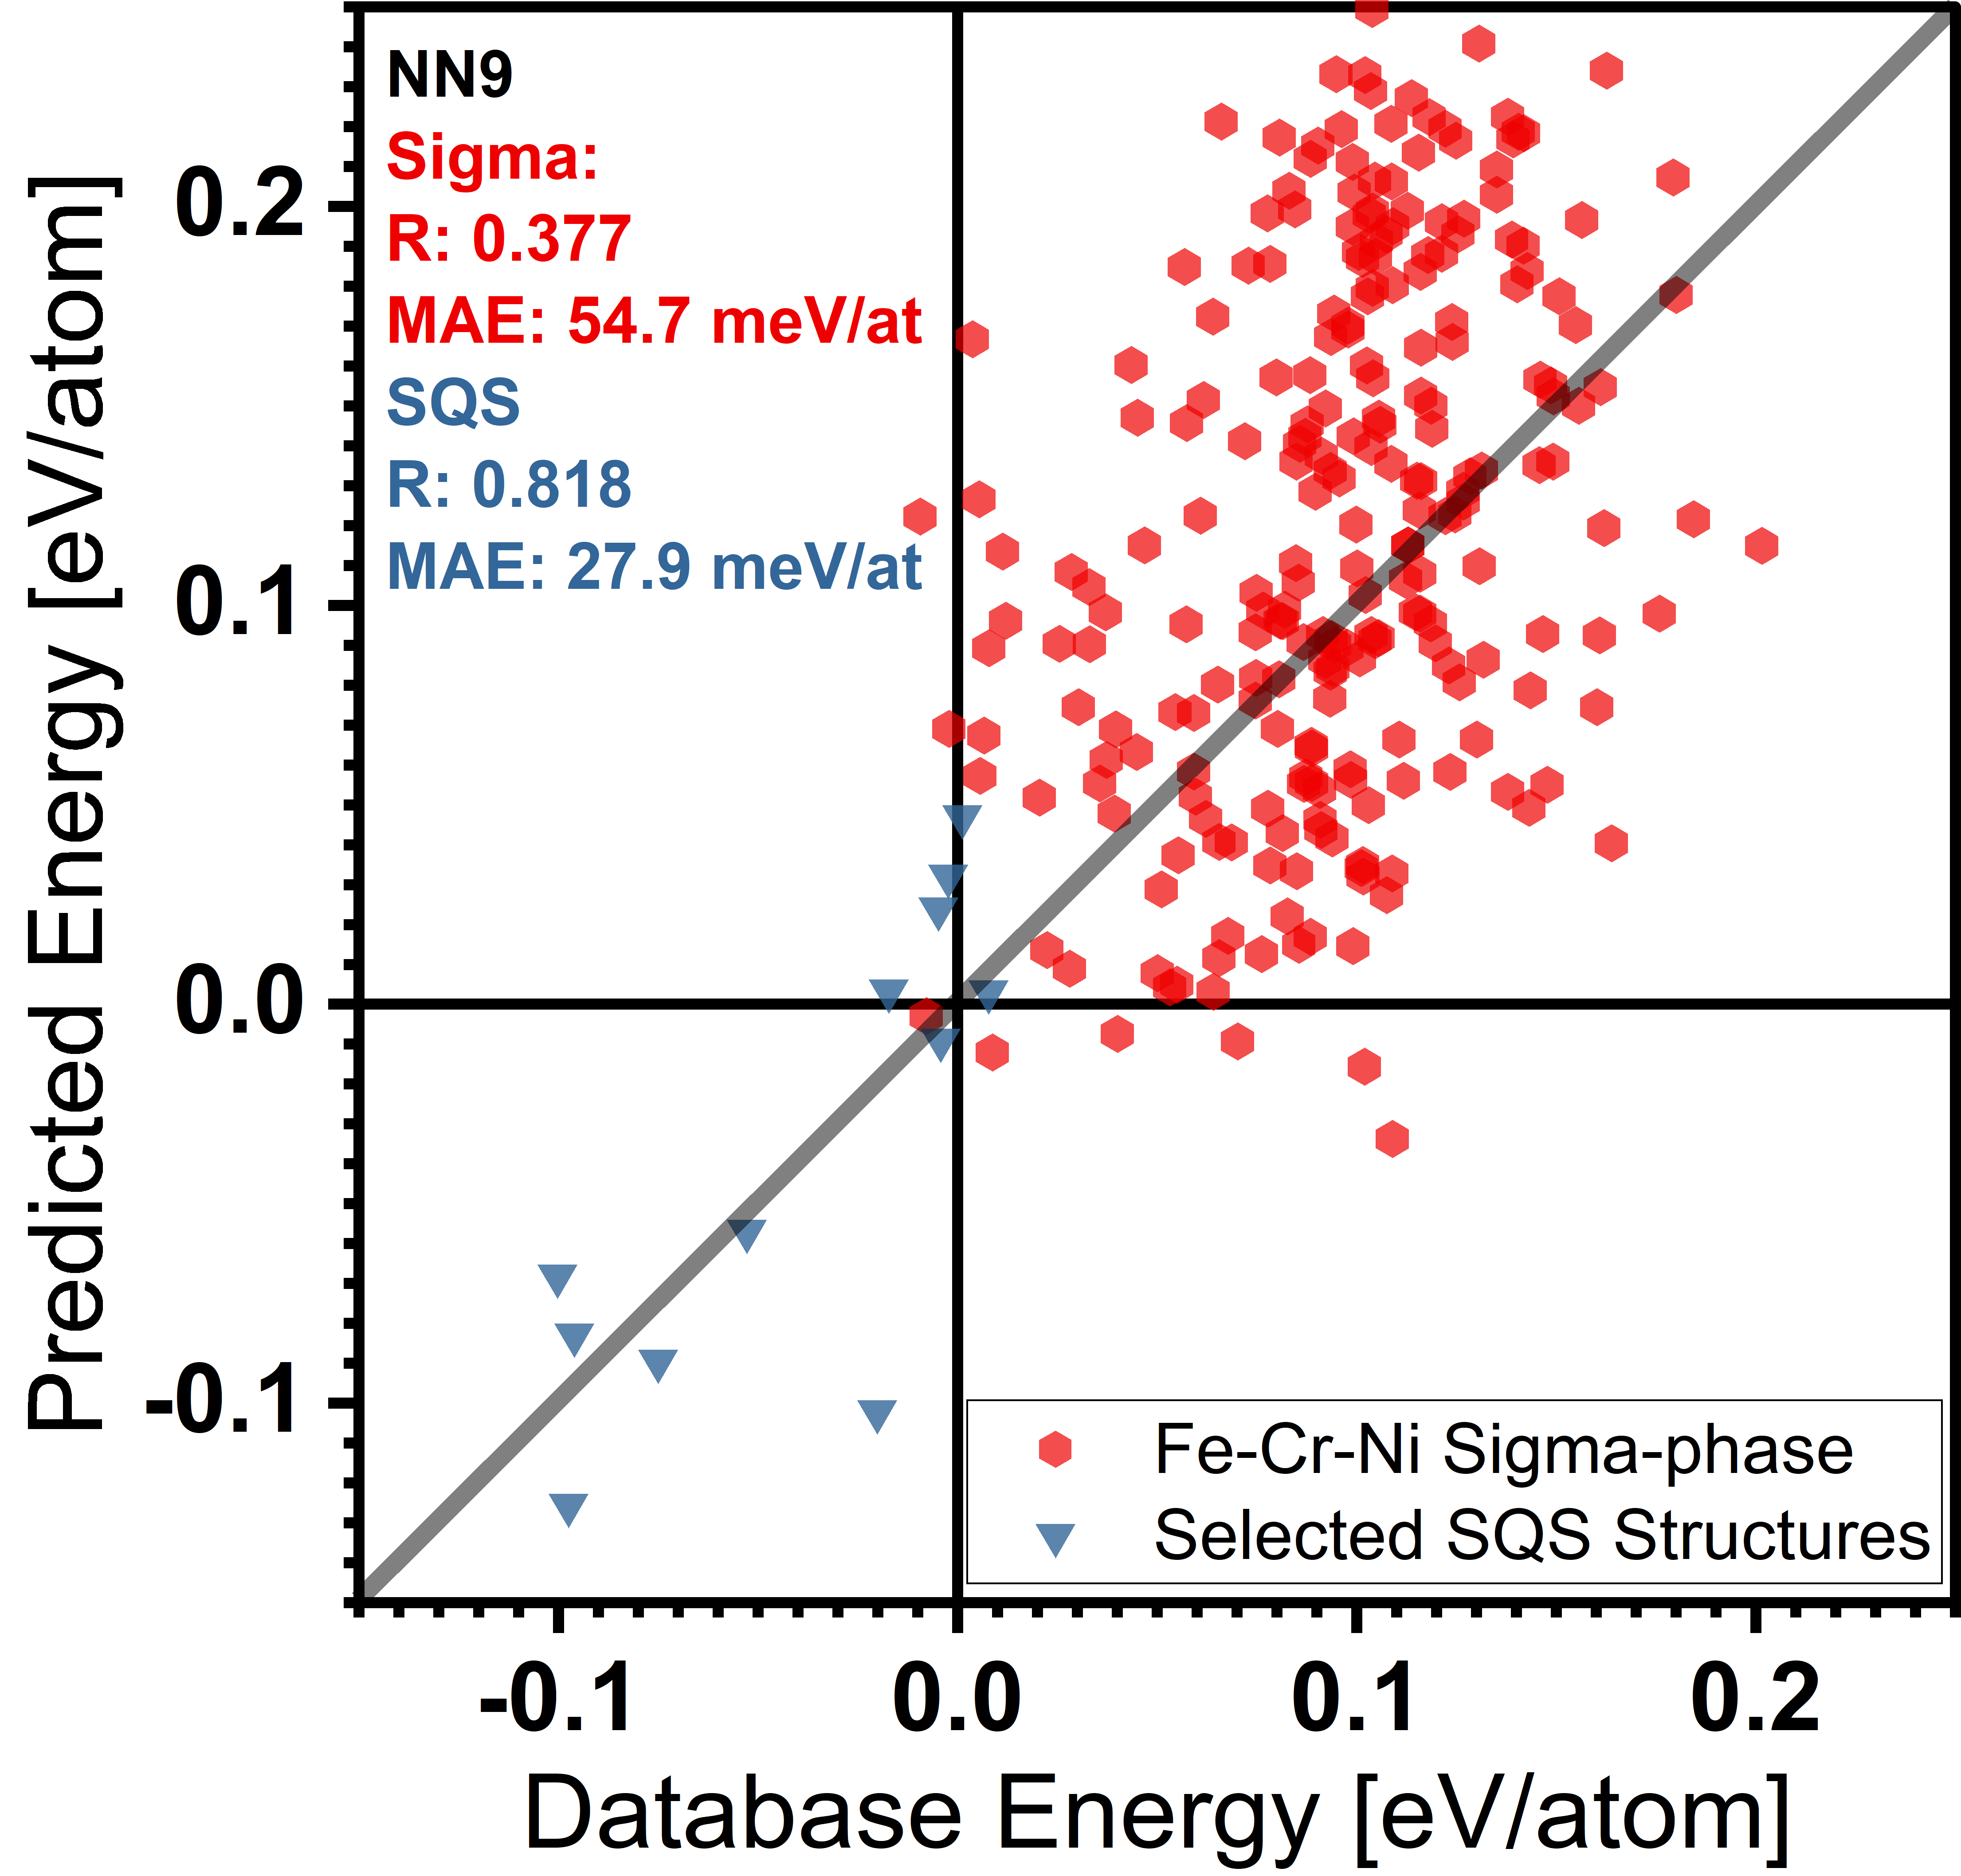
\includegraphics[width=0.3\textwidth]{sipfenn/NN9_sigmasqs.png}
    \hspace{0.03\textwidth}
    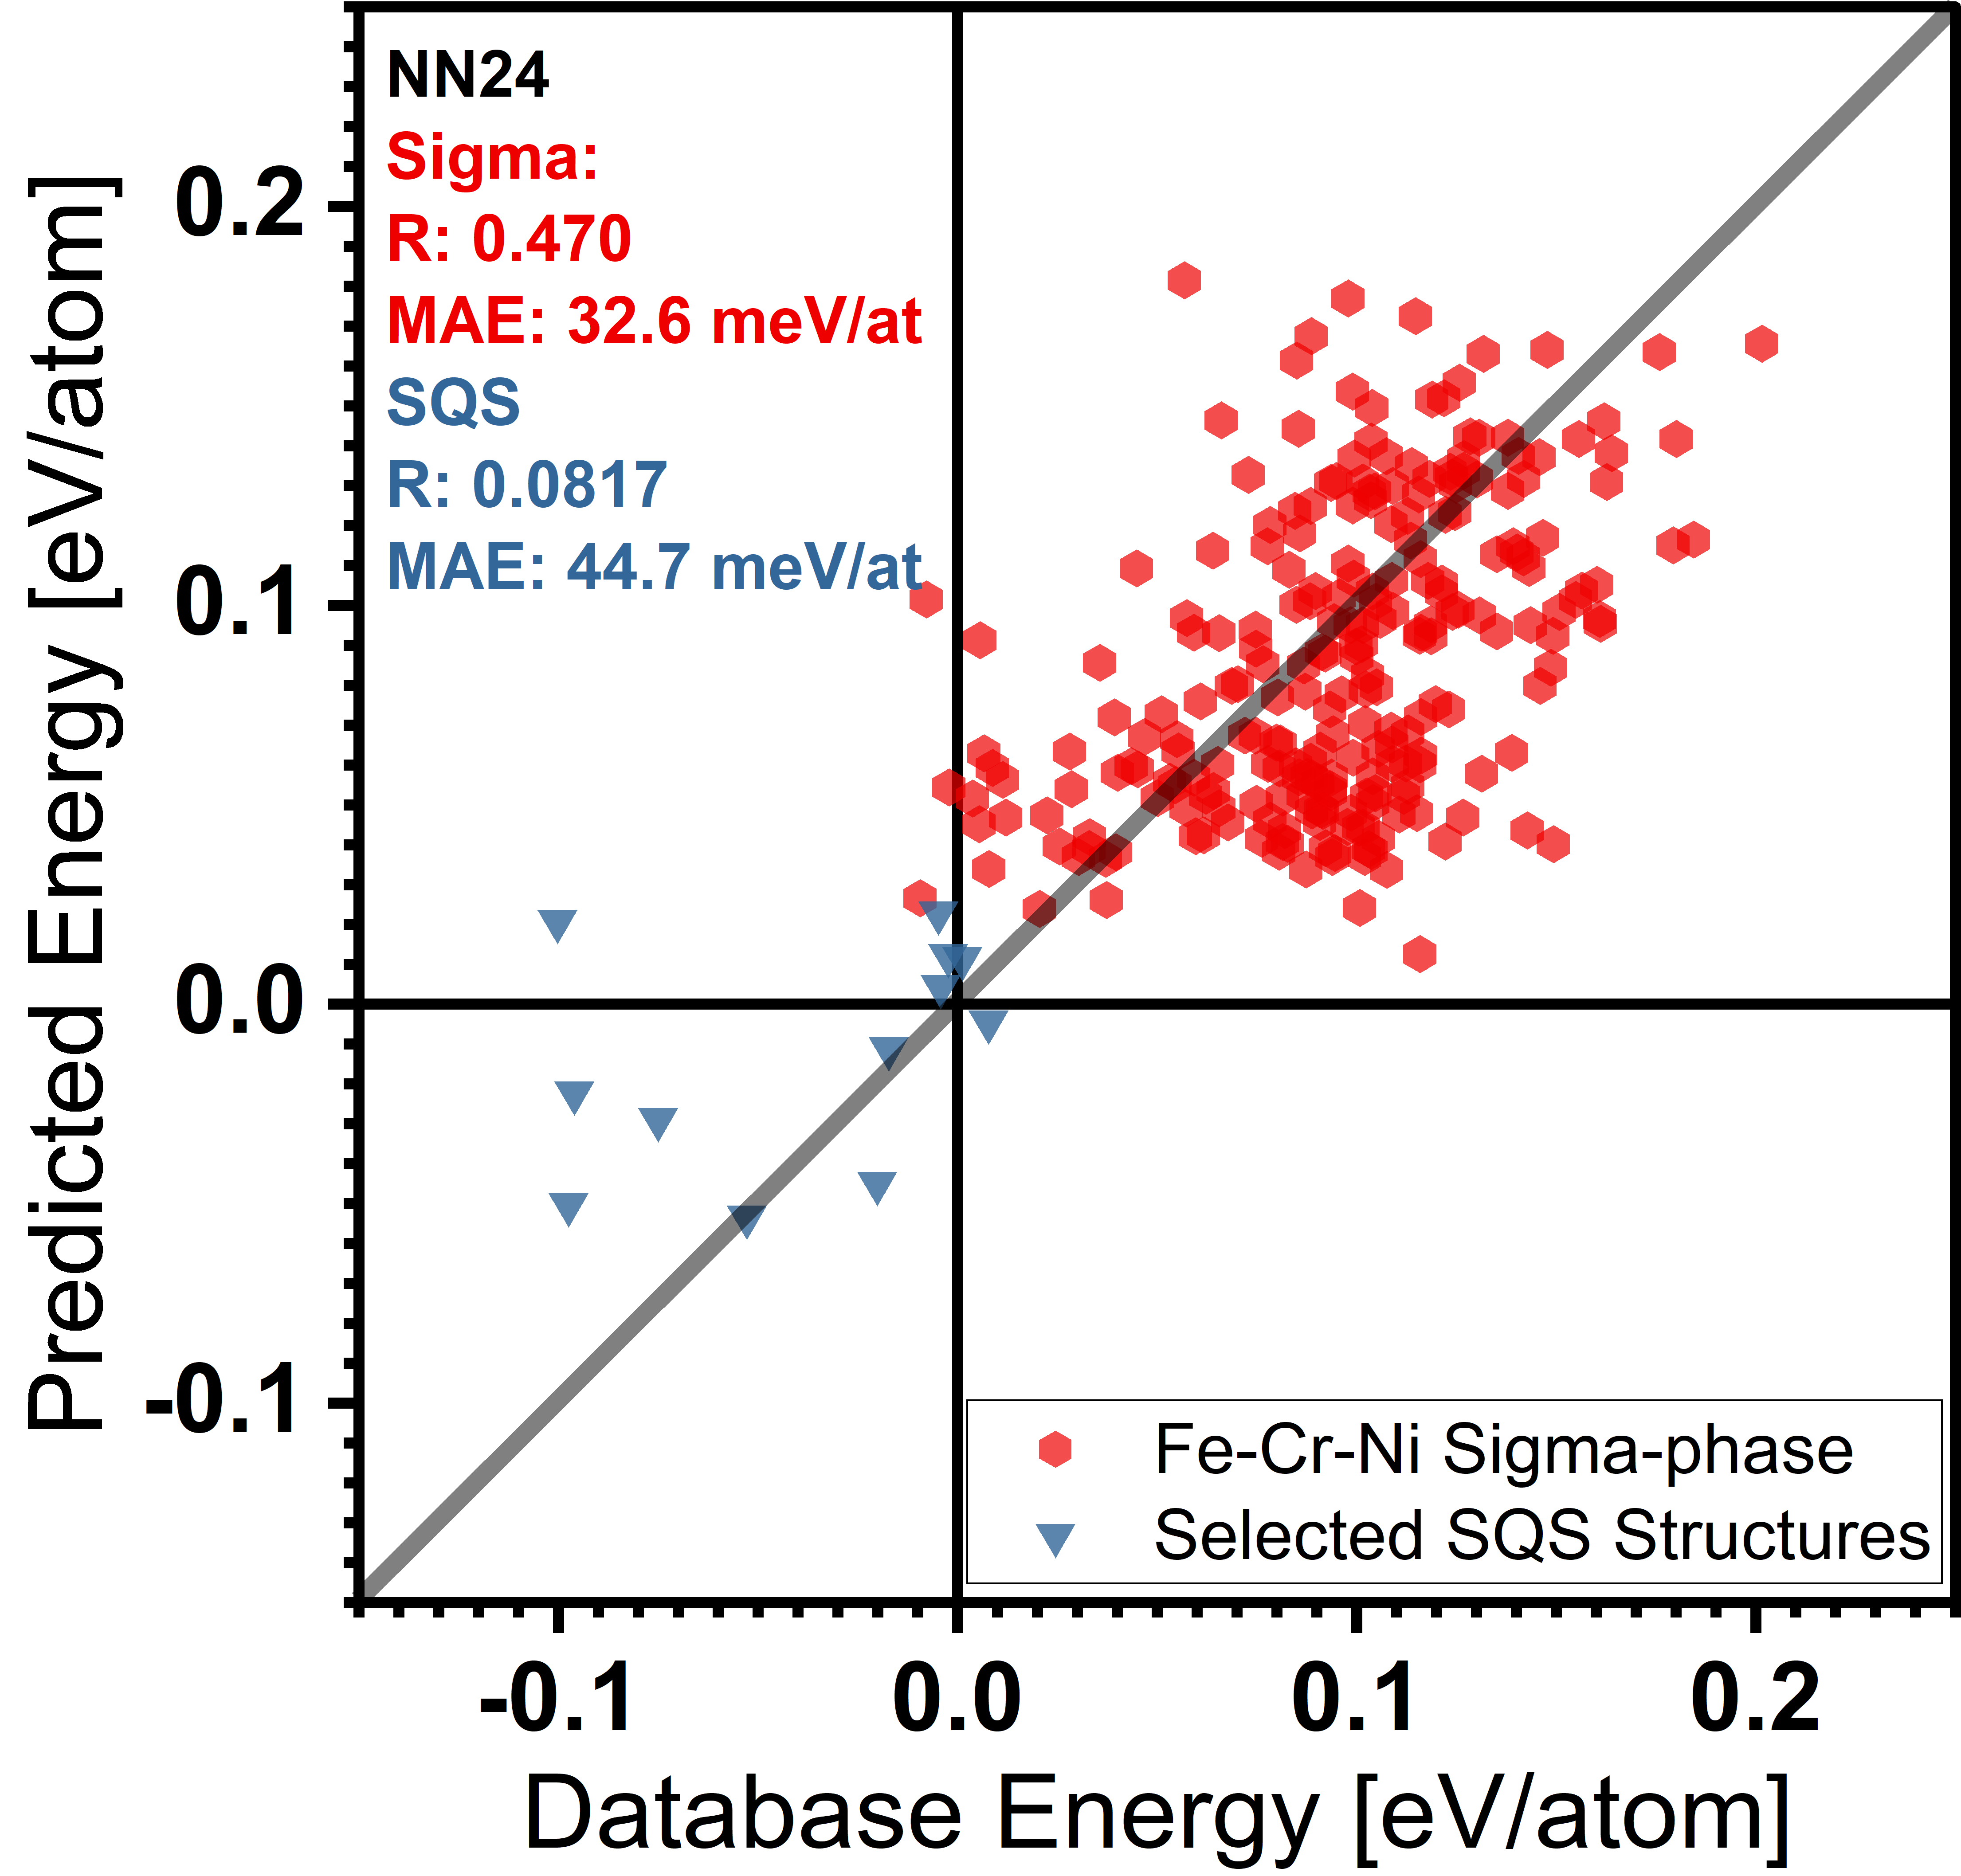
\includegraphics[width=0.3\textwidth]{sipfenn/NN24_sigmasqs.png}
    \hspace{0.03\textwidth}
    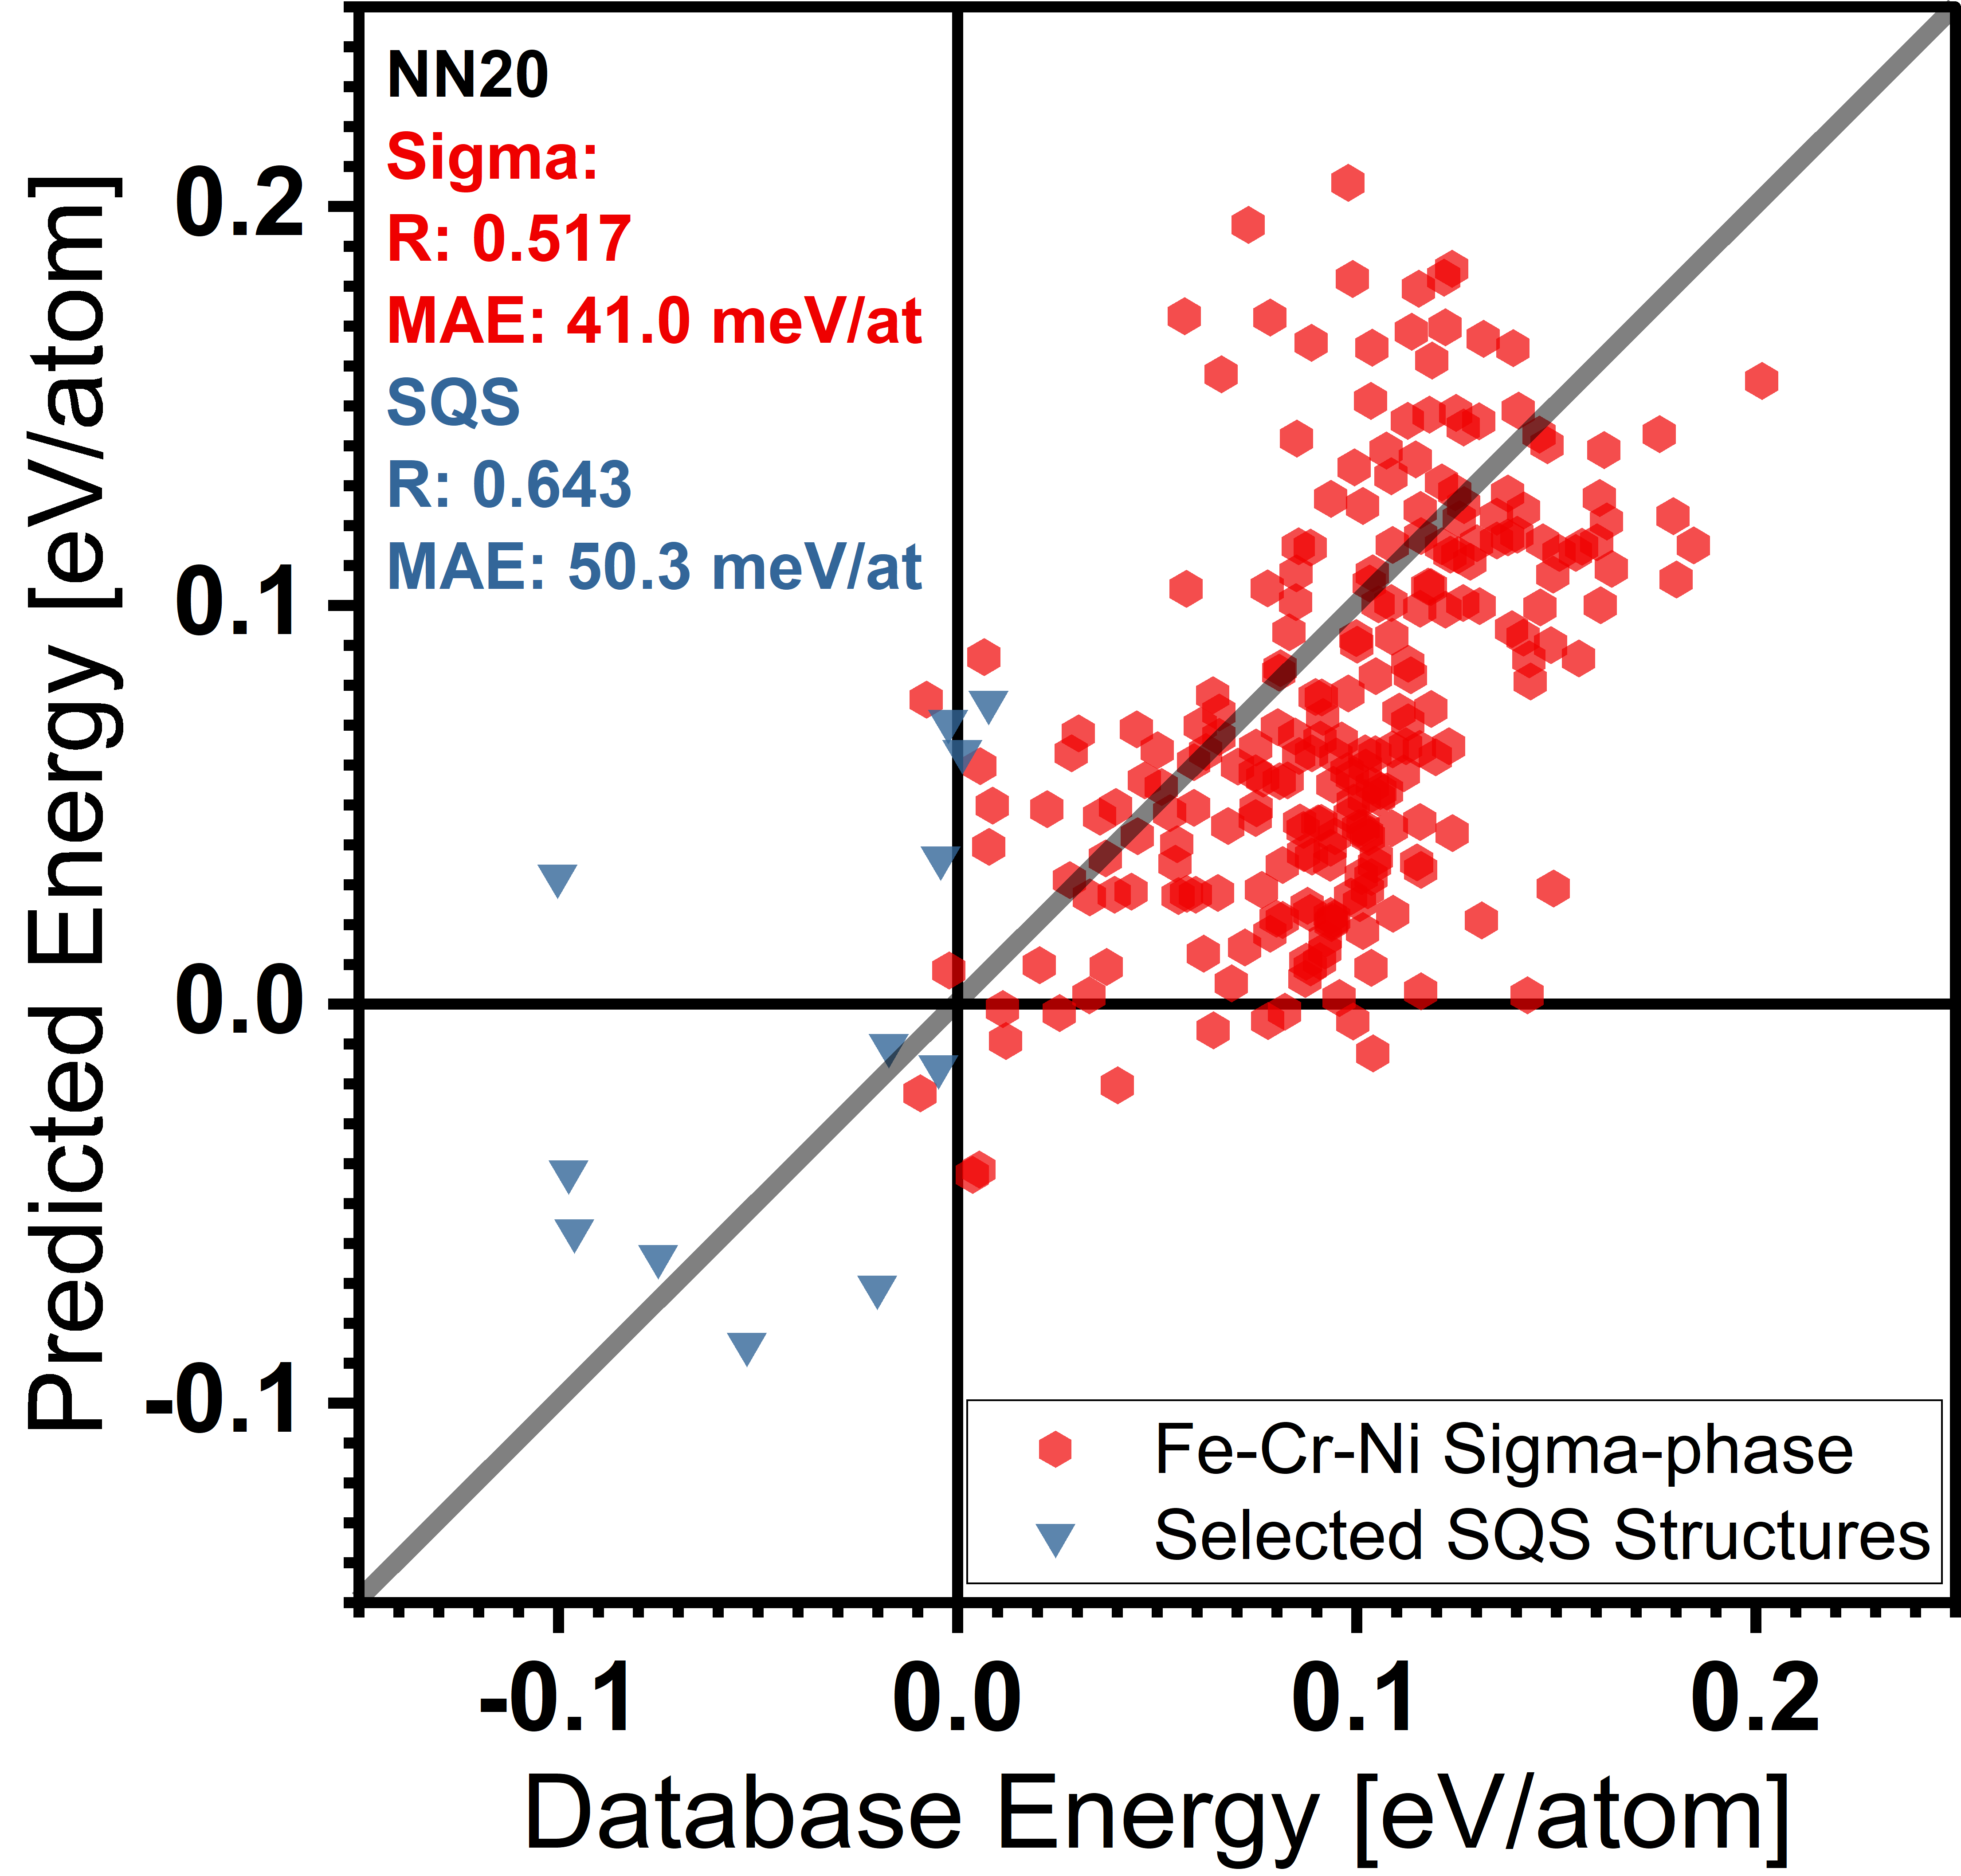
\includegraphics[width=0.3\textwidth]{sipfenn/NN20_sigmasqs.png}
    \caption{Performance of 3 selected neural networks on non-OQMD data described in \ref{sipfenn:sssec:Data}. Evaluated on (red) Fe-Cr-Ni $\sigma$-phase and (blue) SQS dataset. Networks organized by columns; optimized for (left) OQMD performance, (middle) predicting new materials, (right) size-constrained applications. Internally in the code, they are designated as NN9, NN20, and NN24 respectively.}
    \label{sipfenn:fig:sigmasqsperformance}
\end{figure}

While all three models performed at around the same MAE level as for the OQMD, network optimized for new materials, the NN20 and NN24, performed better in the non-OQMD test cases of interest, providing major increases in correlations, significant for ranking of end-member configurations, except for 4 SQS configurations which were underestimated. The Pearson correlation slightly decreased in the first case and slightly increased in the second case. In both cases, the mean absolute error decreased by about 20\% compared to the OQMD-optimized model.


\subsection{Transfer Learning Capability} \label{sipfenn:ssec:transferlearningresults}
In this section, the technique of transfer learning is considered. It has been observed among deep learning models across a variety of domains \cite{tan2018survey,cirecsan2012transfer,chang2017unsupervised,george2018deep} and refers the to the ability of properly trained deep learning models to `transfer' their knowledge to related tasks. In the least complex approach, one does this by simply 'fine-tuning' the parameters of the model using new training data (from the new task). This methodology has shown in practice that deep neural networks are often able to transfer knowledge between different but related tasks. Such a problem is analogous to many others in materials science, where general knowledge is used to make meaningful statements without statistically significant patterns in locally available data. 

It is shown that a network trained on the OQMD database, which covers a broad yet limited spectrum of materials, can be quickly adjusted to materials outside of this spectrum with very little additional cost relative to the initial training. Specifically, the transfer learning capability of a network trained in this way on the set of all (243) Fe-Ni-Cr $\sigma$-phase 5-sublattice model endmembers, described in \ref{sipfenn:sssec:Data}, was tested. The ML model was first trained on a broad and general material dataset (OQMD) and then further trained (i.e., re-trained) for a given number of rounds on the new data (Fe-Ni-Cr $\sigma$-phase dataset) to adapt to the new system, while still conserving its broad knowledge, and can be thought of as fine-tuning a model to improve extrapolation outside of a prior knowledge space. 

In order to achieve good performance, both the number of rounds and the learning rate have to be optimized. This can be accomplished by investigating the dependence of error on the fraction of available data while one of these parameters is fixed. Figure \ref{sipfenn:fig:transfersigmaLR} presents the dependence of transfer learning from new data for different learning rates expressed as fractions of default ADAM learning rate (0.001 shared across a vast majority of software). 

\begin{figure}[H]
    \centering
    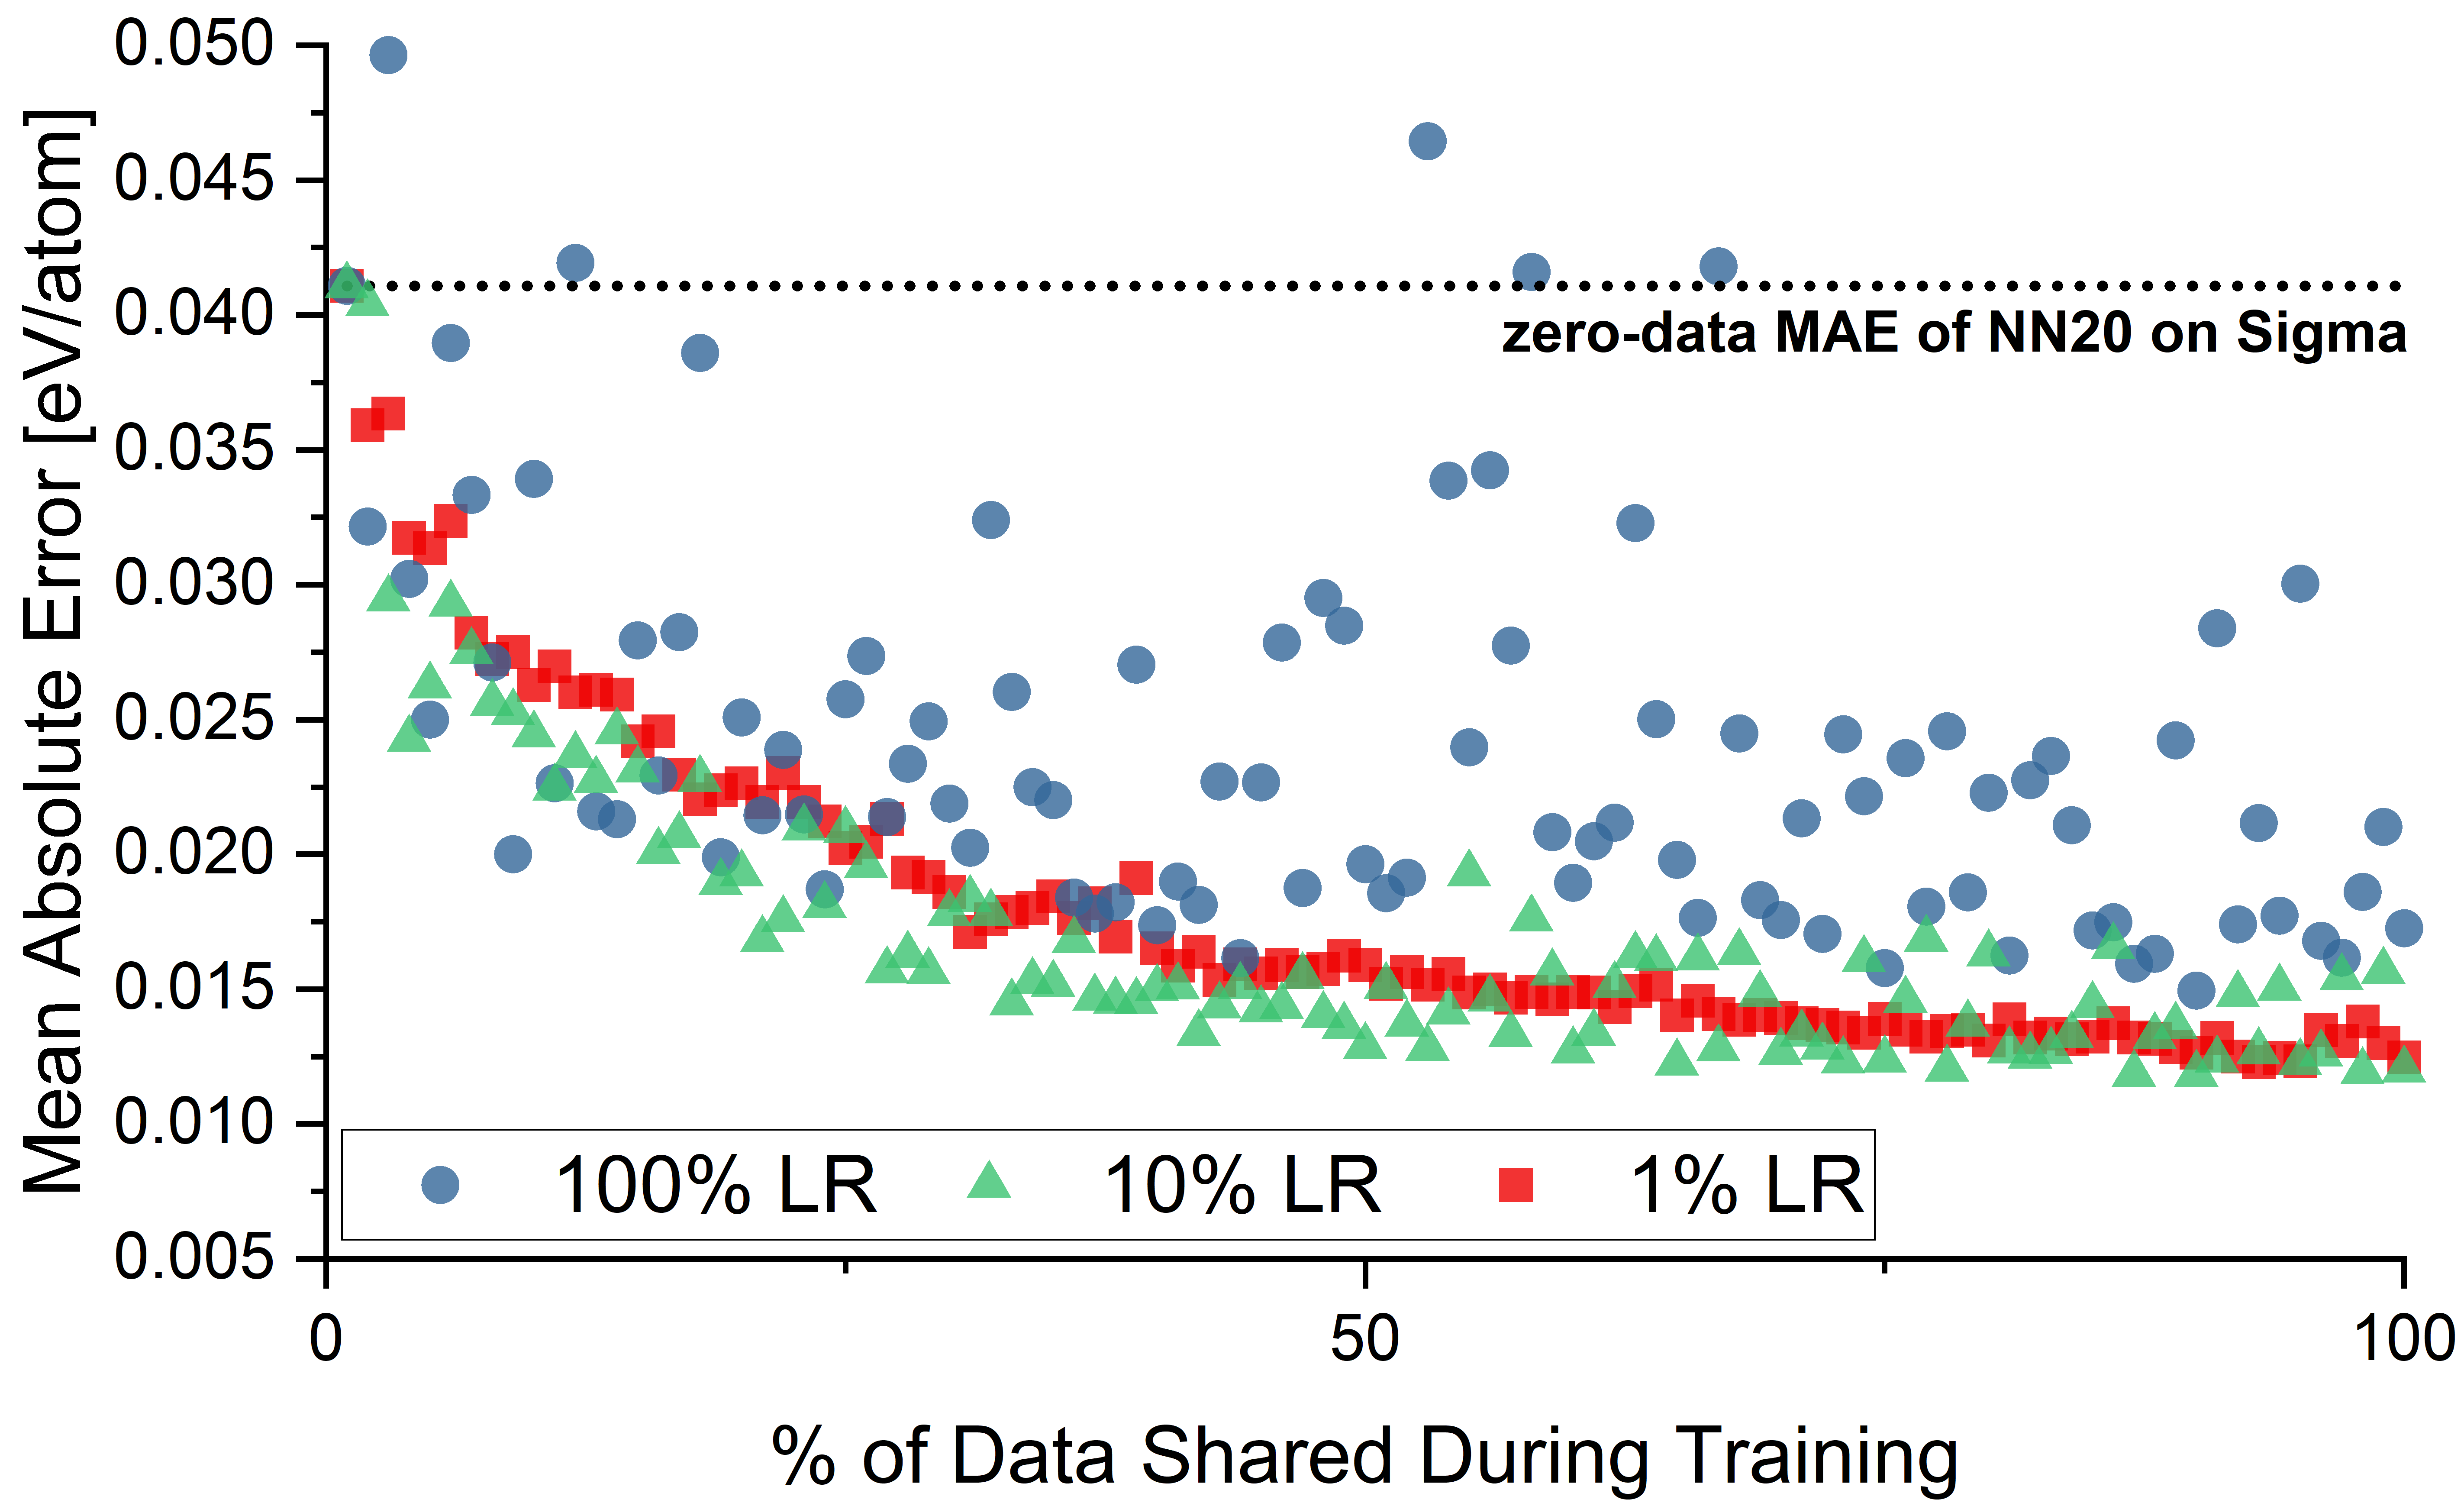
\includegraphics[width=0.6\textwidth]{sipfenn/transferLearning_MAE_vs_LearningRate.png}
    \caption{MAE evolution of NN20 model re-trained for 25 additional rounds on an increasing fraction of data from Fe-Cr-Ni $\sigma-$dataset. Presents the dependence of transfer learning from new data for different learning rates expressed as fractions of default ADAM learning rate (0.001).}
    \vspace{-12pt}
    \label{sipfenn:fig:transfersigmaLR}
\end{figure}

As shown, in this case, the default learning rate (100\%)cannot be used for the transfer learning as it will adjust network parameters in both an unreliable and detrimental fashion, resulting in poor performance on the whole system of interest (both training and test sets) as shown in Figure \ref{sipfenn:fig:transfersigmaLR}. The same behavior would be observed if the process were conducted using an automated model design available in software such as \texttt{MATLAB} or \texttt{Mathematica}. The 10\% learning rate provided reliable enough outcomes and allowed a better performance improvement given little data, relative to using a 1\% learning rate (relative to the default). The second parameter to be optimized was the number of re-training rounds, as presented in Figure \ref{sipfenn:fig:transfersigmaARR}.

\begin{figure}[H]
    \centering
    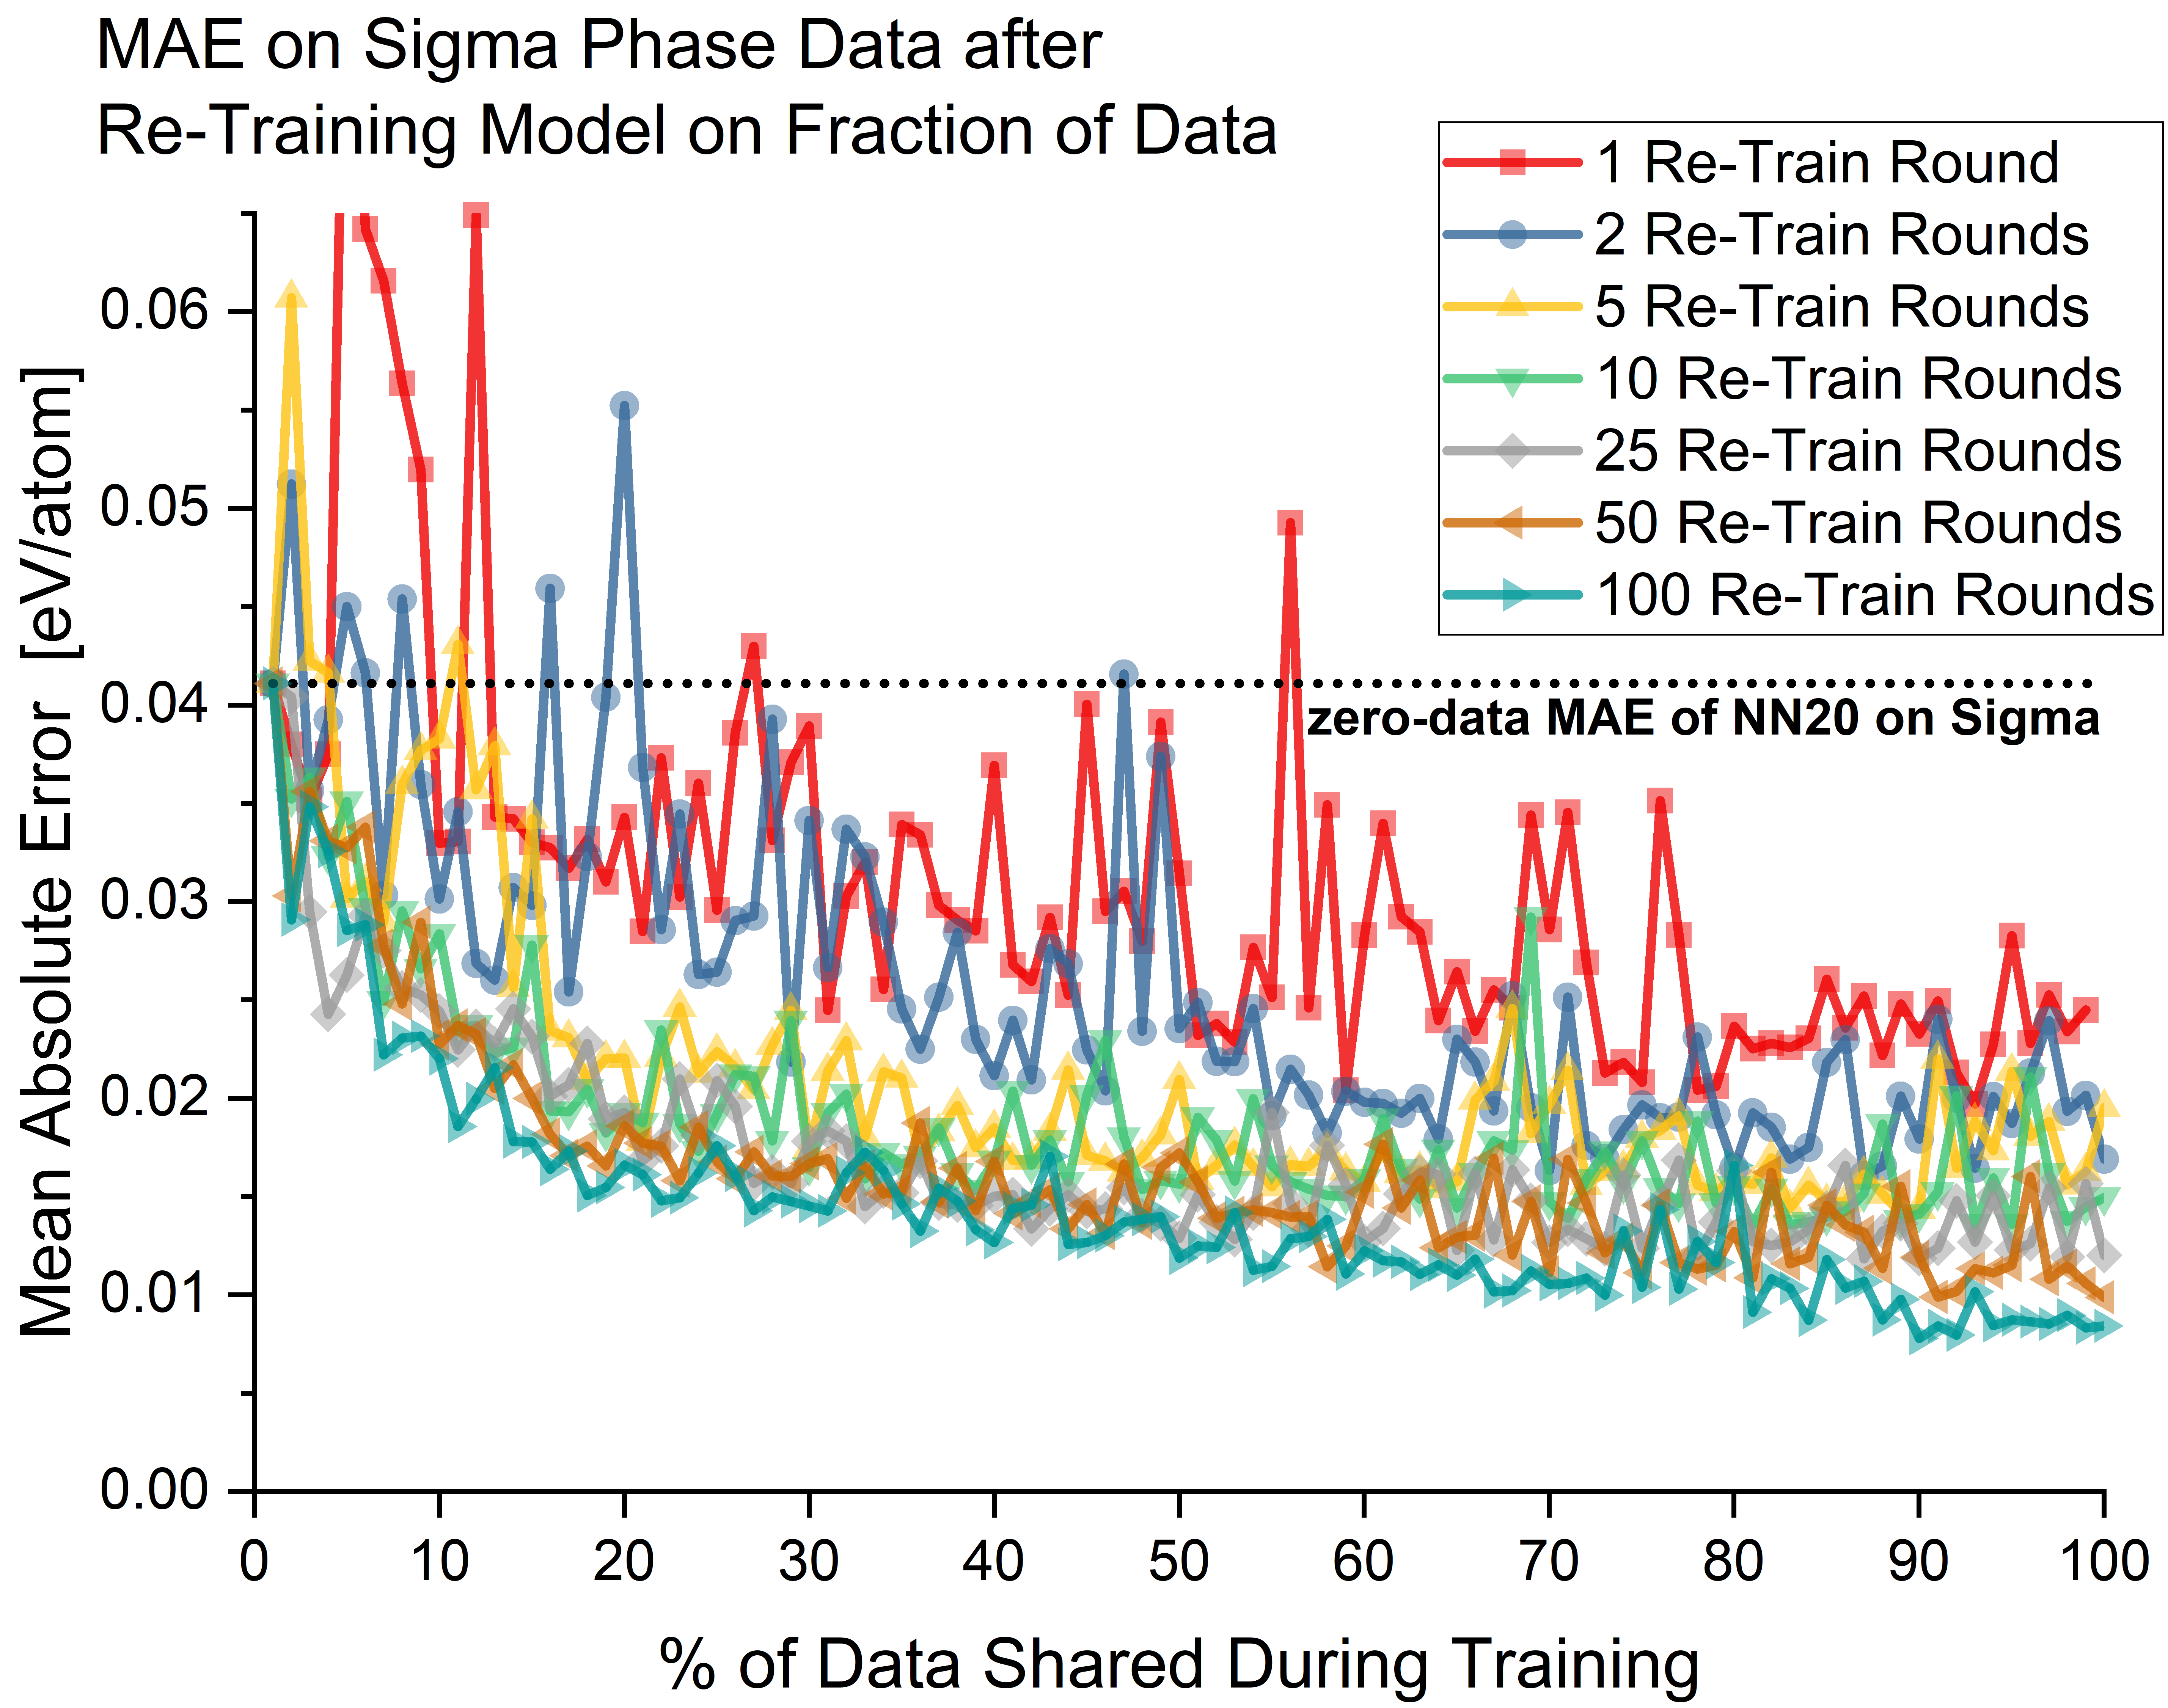
\includegraphics[width=0.48\textwidth]{sipfenn/transferLearning_MAE_vs_rounds.png}
    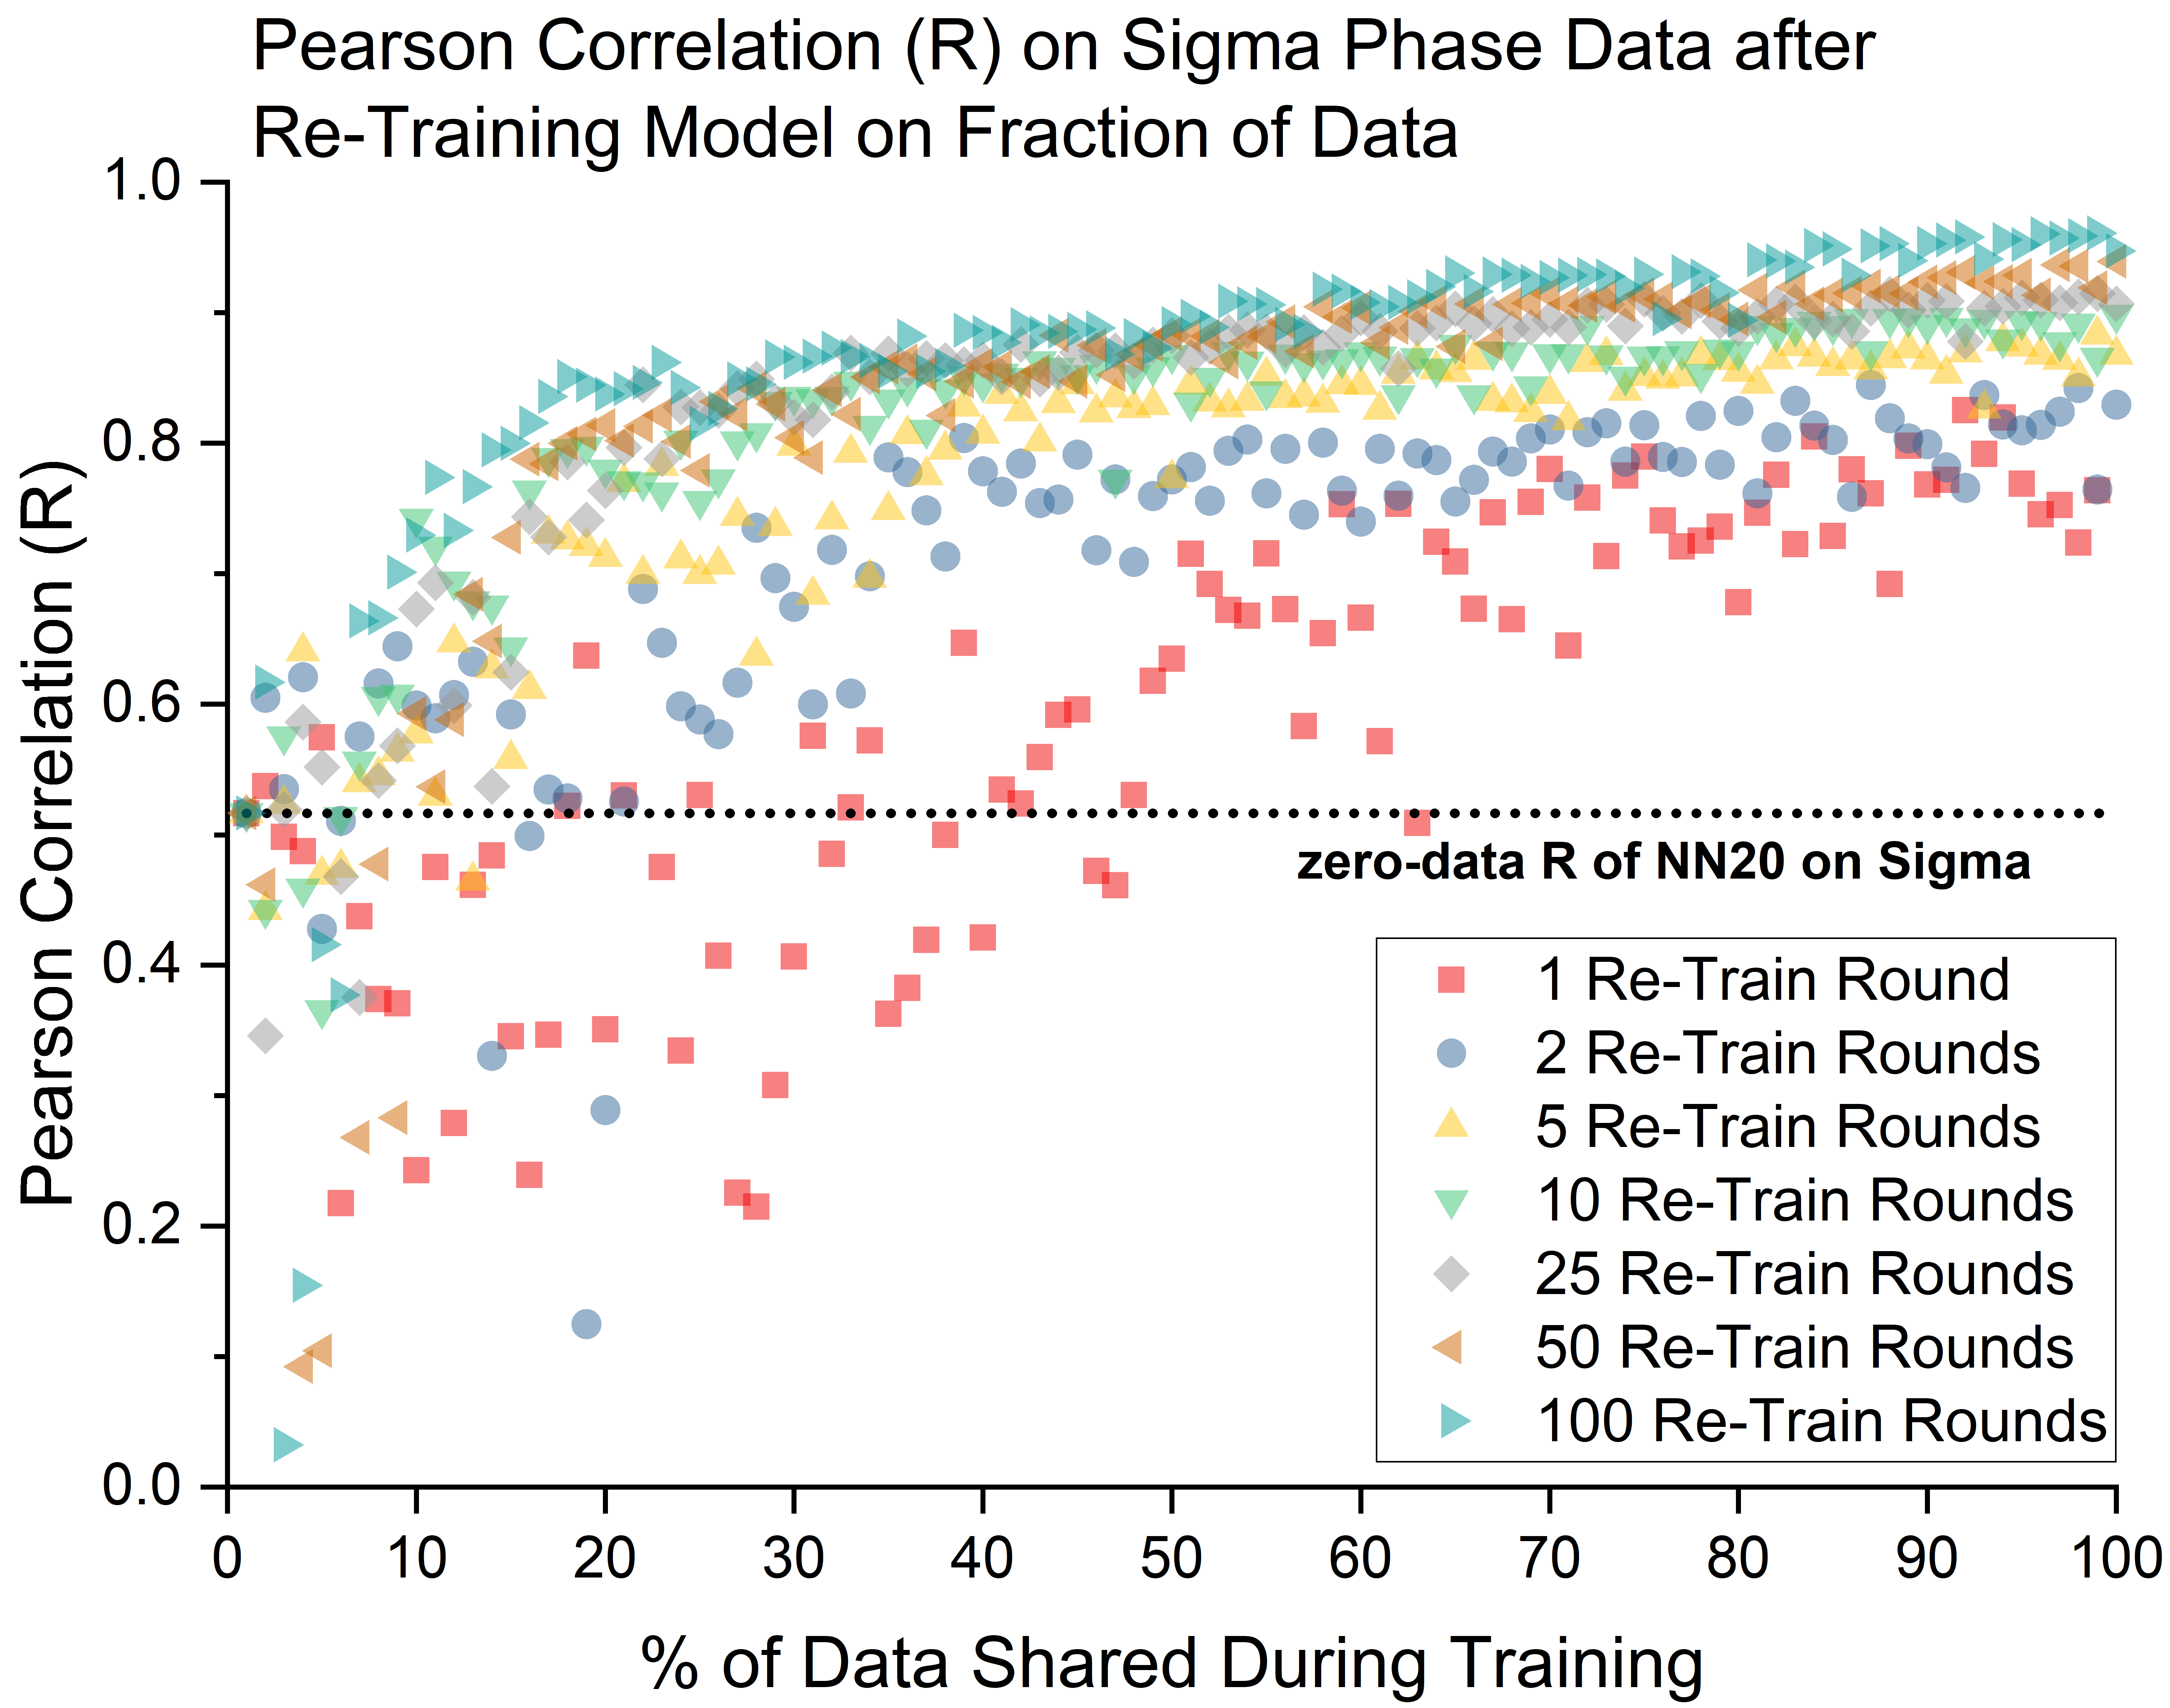
\includegraphics[width=0.48\textwidth]{sipfenn/transferLearning_R.png}
    \caption{MAE and Person correlation (R) evolution of NN20 model re-trained at 10\% learning rate on an increasing fraction of data from Fe-Cr-Ni $\sigma-$dataset. Presents the dependence of transfer learning from new data for different re-training rounds numbers.}
    \vspace{-12pt}
    \label{sipfenn:fig:transfersigmaARR}
\end{figure}

Figure \ref{sipfenn:fig:transfersigmaARR} shows that use of too few retraining rounds causes unreliable outcomes, while too many causes overfitting for low amounts of new data. In the case of Fe-Cr-Ni $\sigma-$dataset, retraining for 10 or 25 rounds provides balanced results across the whole dataset. With parameters for the process set to 10\% learning rate and 25 additional rounds, the performance can be evaluated graphically, as presented in Figure \ref{sipfenn:fig:transfersigma}.

\begin{figure}[H]
    \centering
    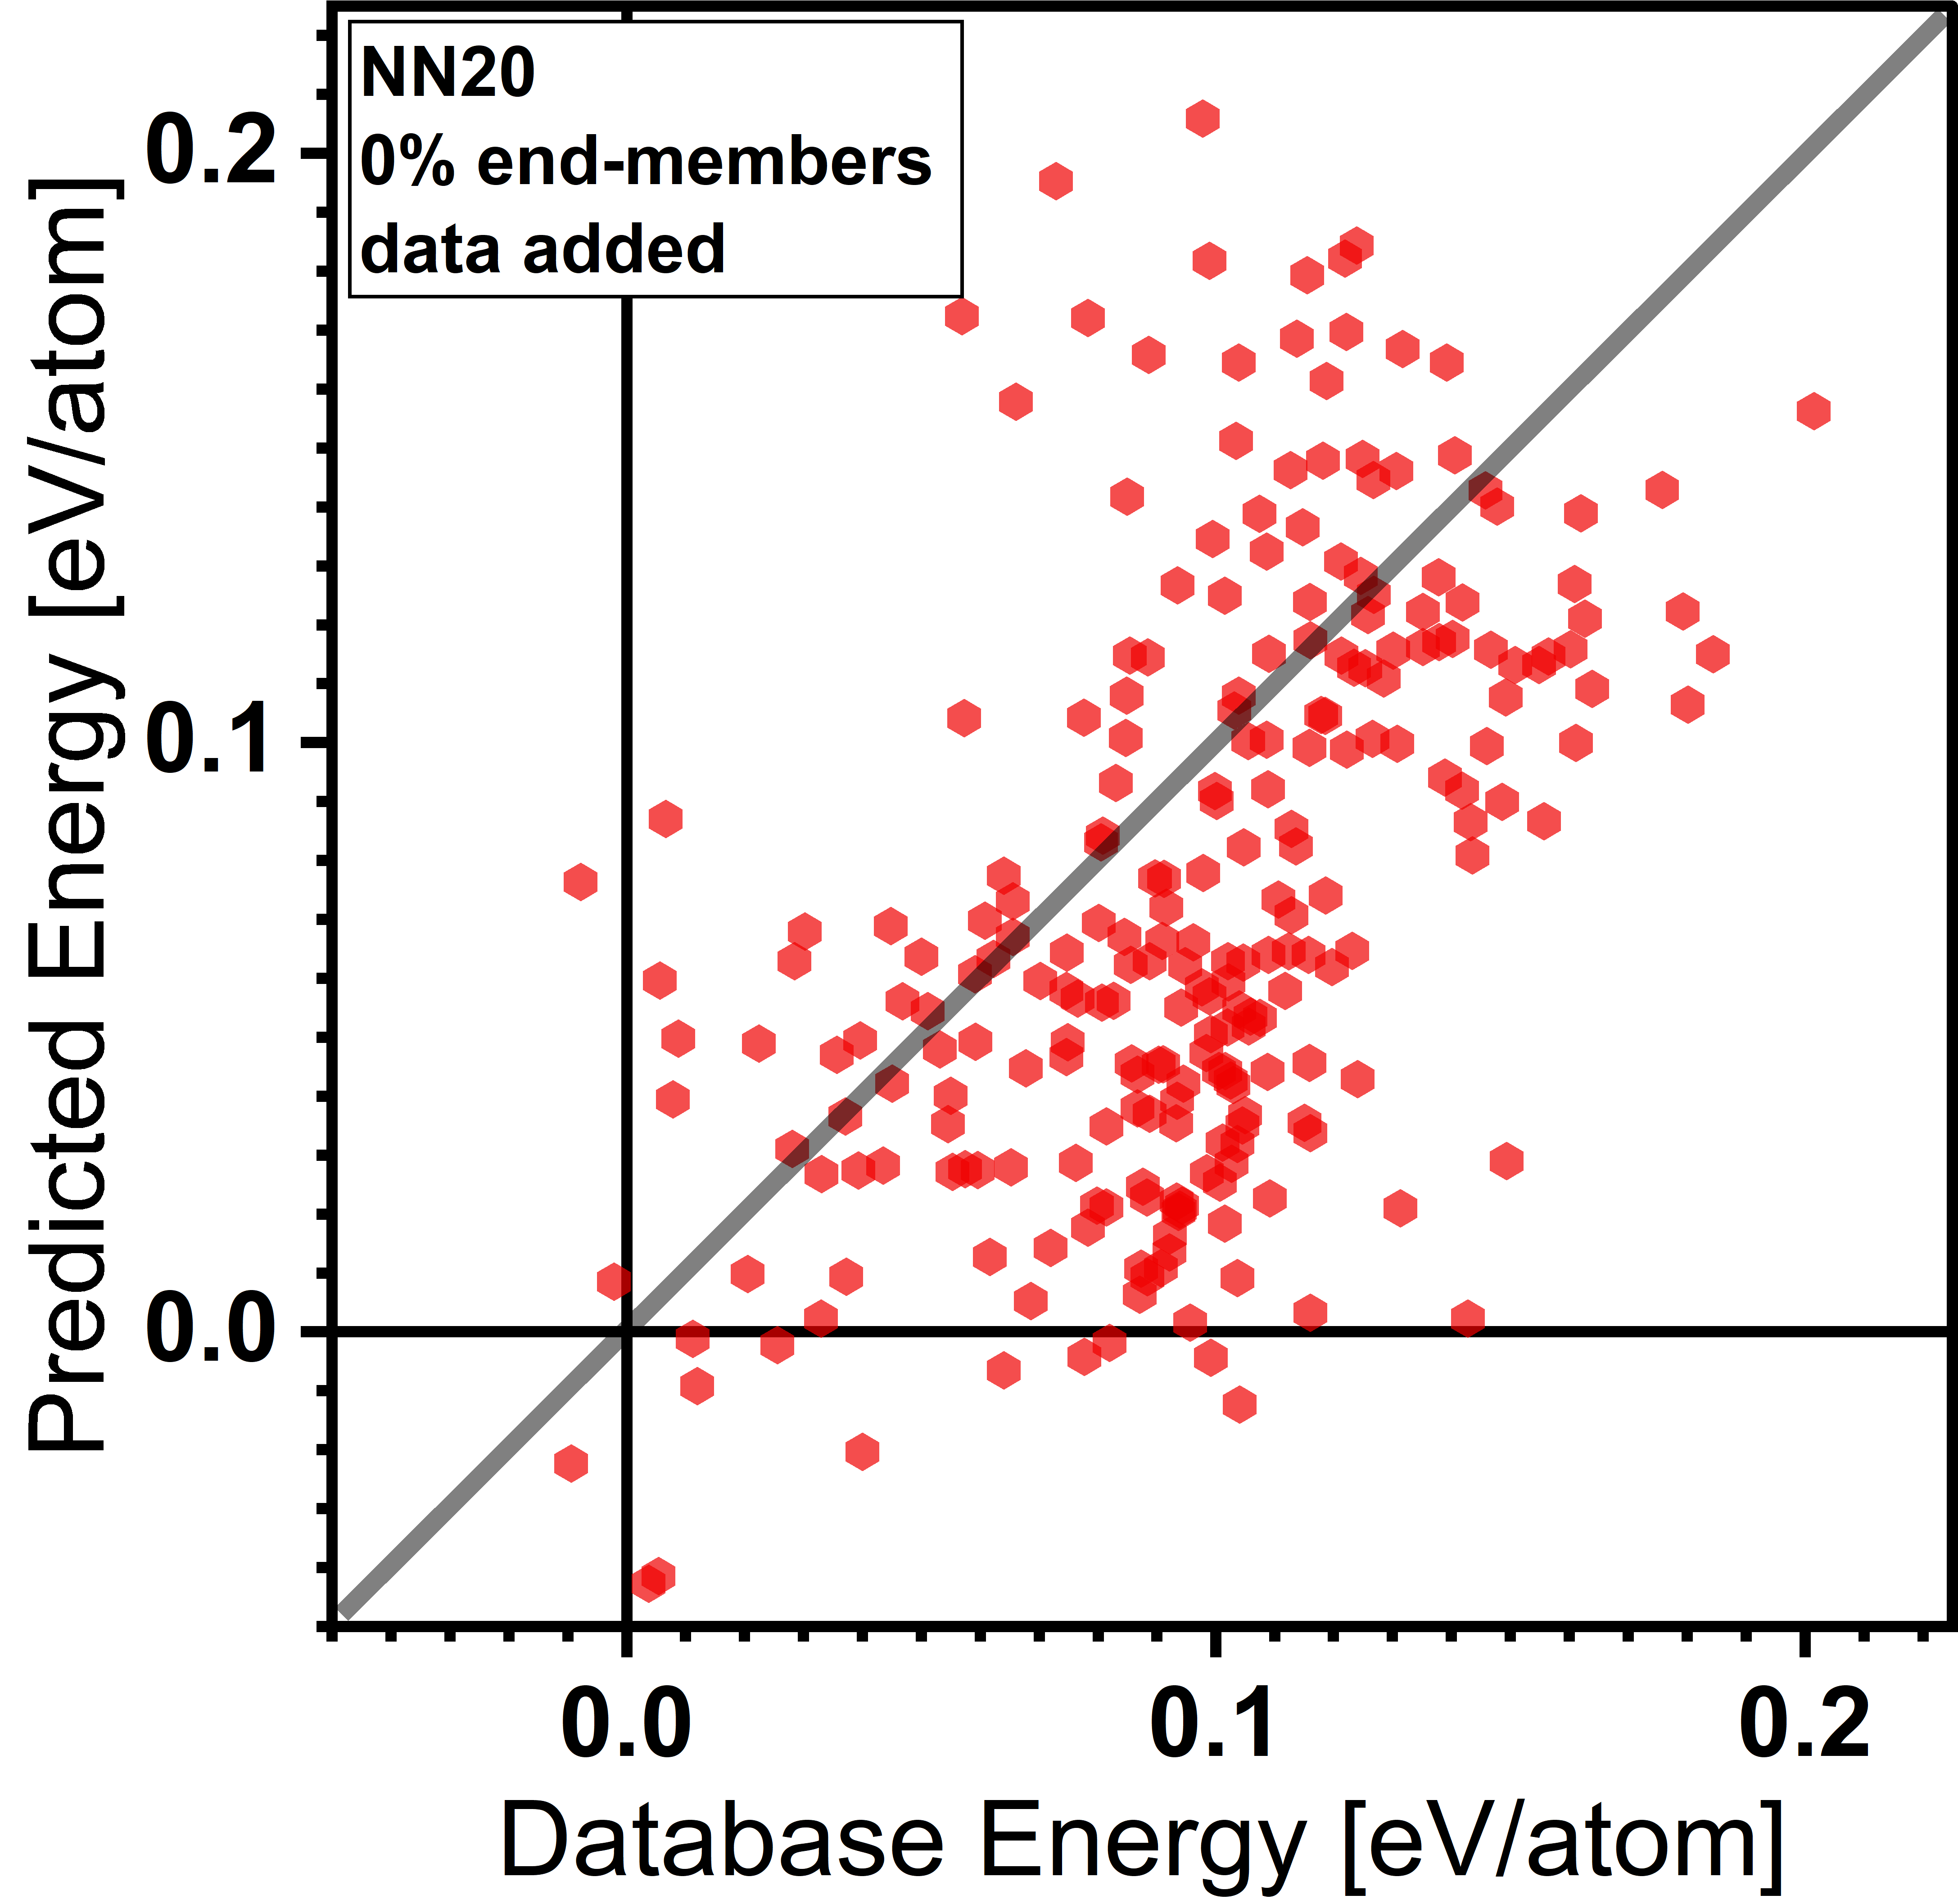
\includegraphics[width=0.24\textwidth]{sipfenn/NN20_SigmaTransfer_0.png}
    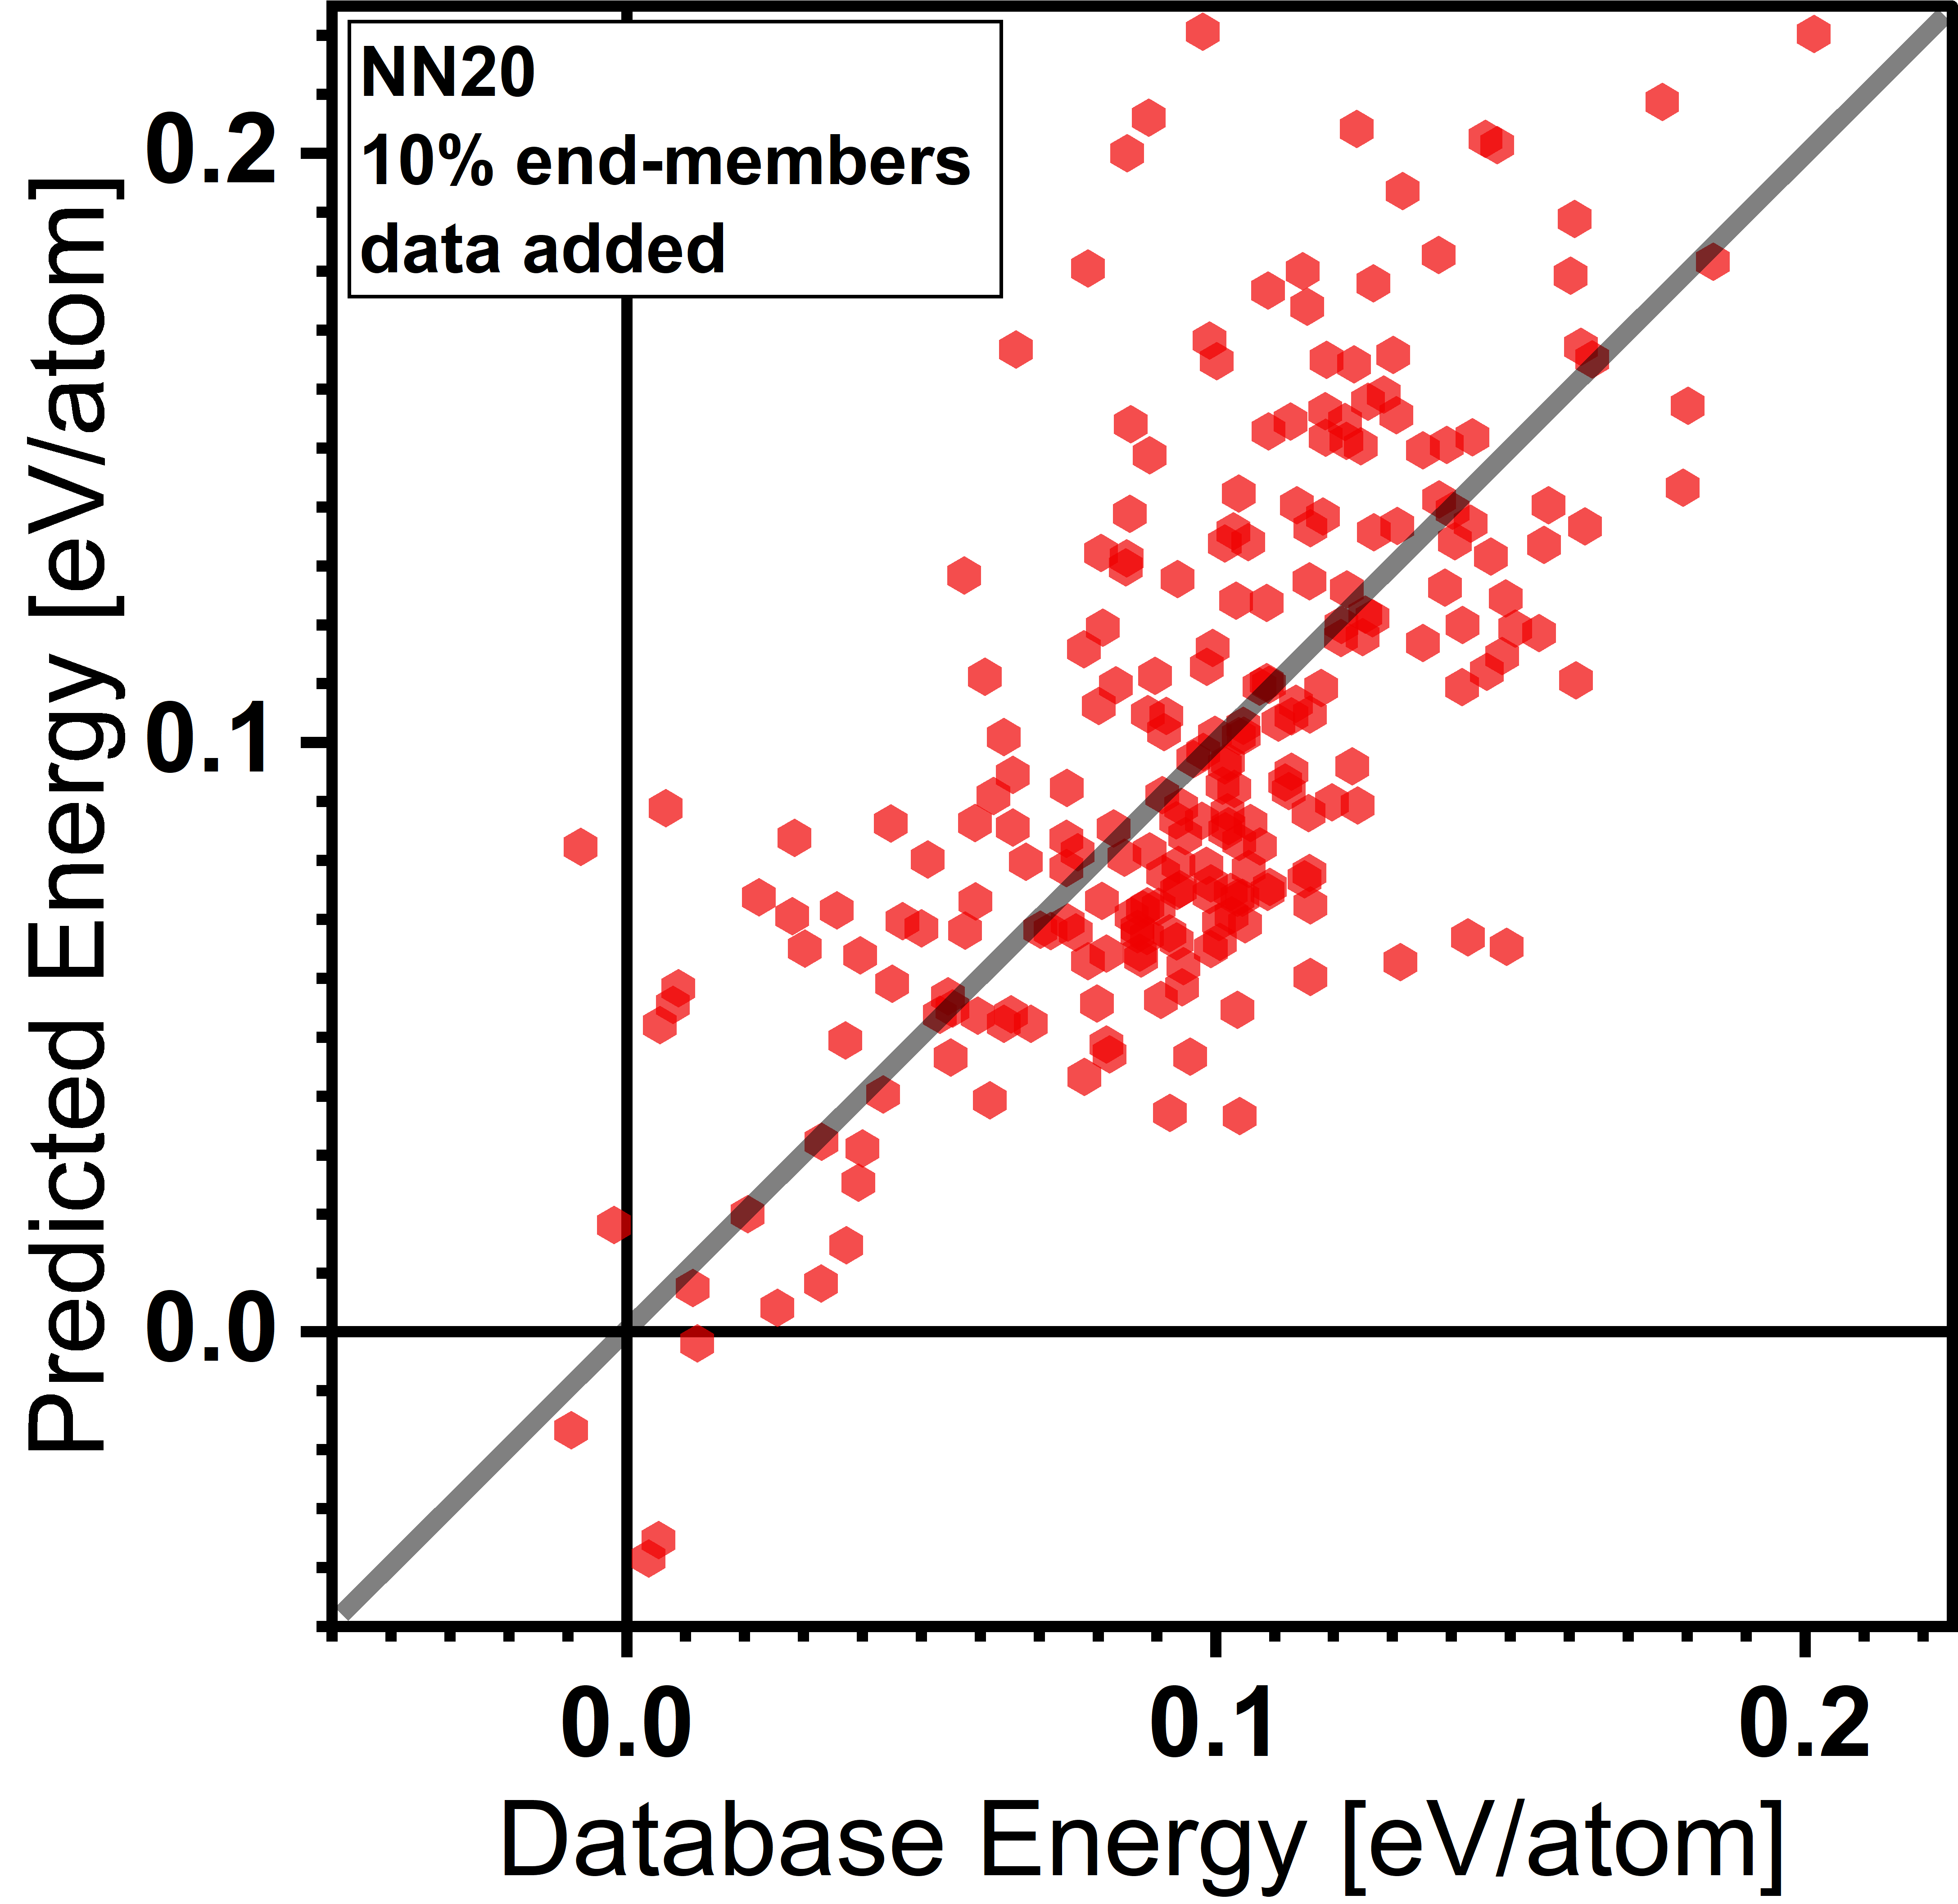
\includegraphics[width=0.24\textwidth]{sipfenn/NN20_SigmaTransfer_1.png}
    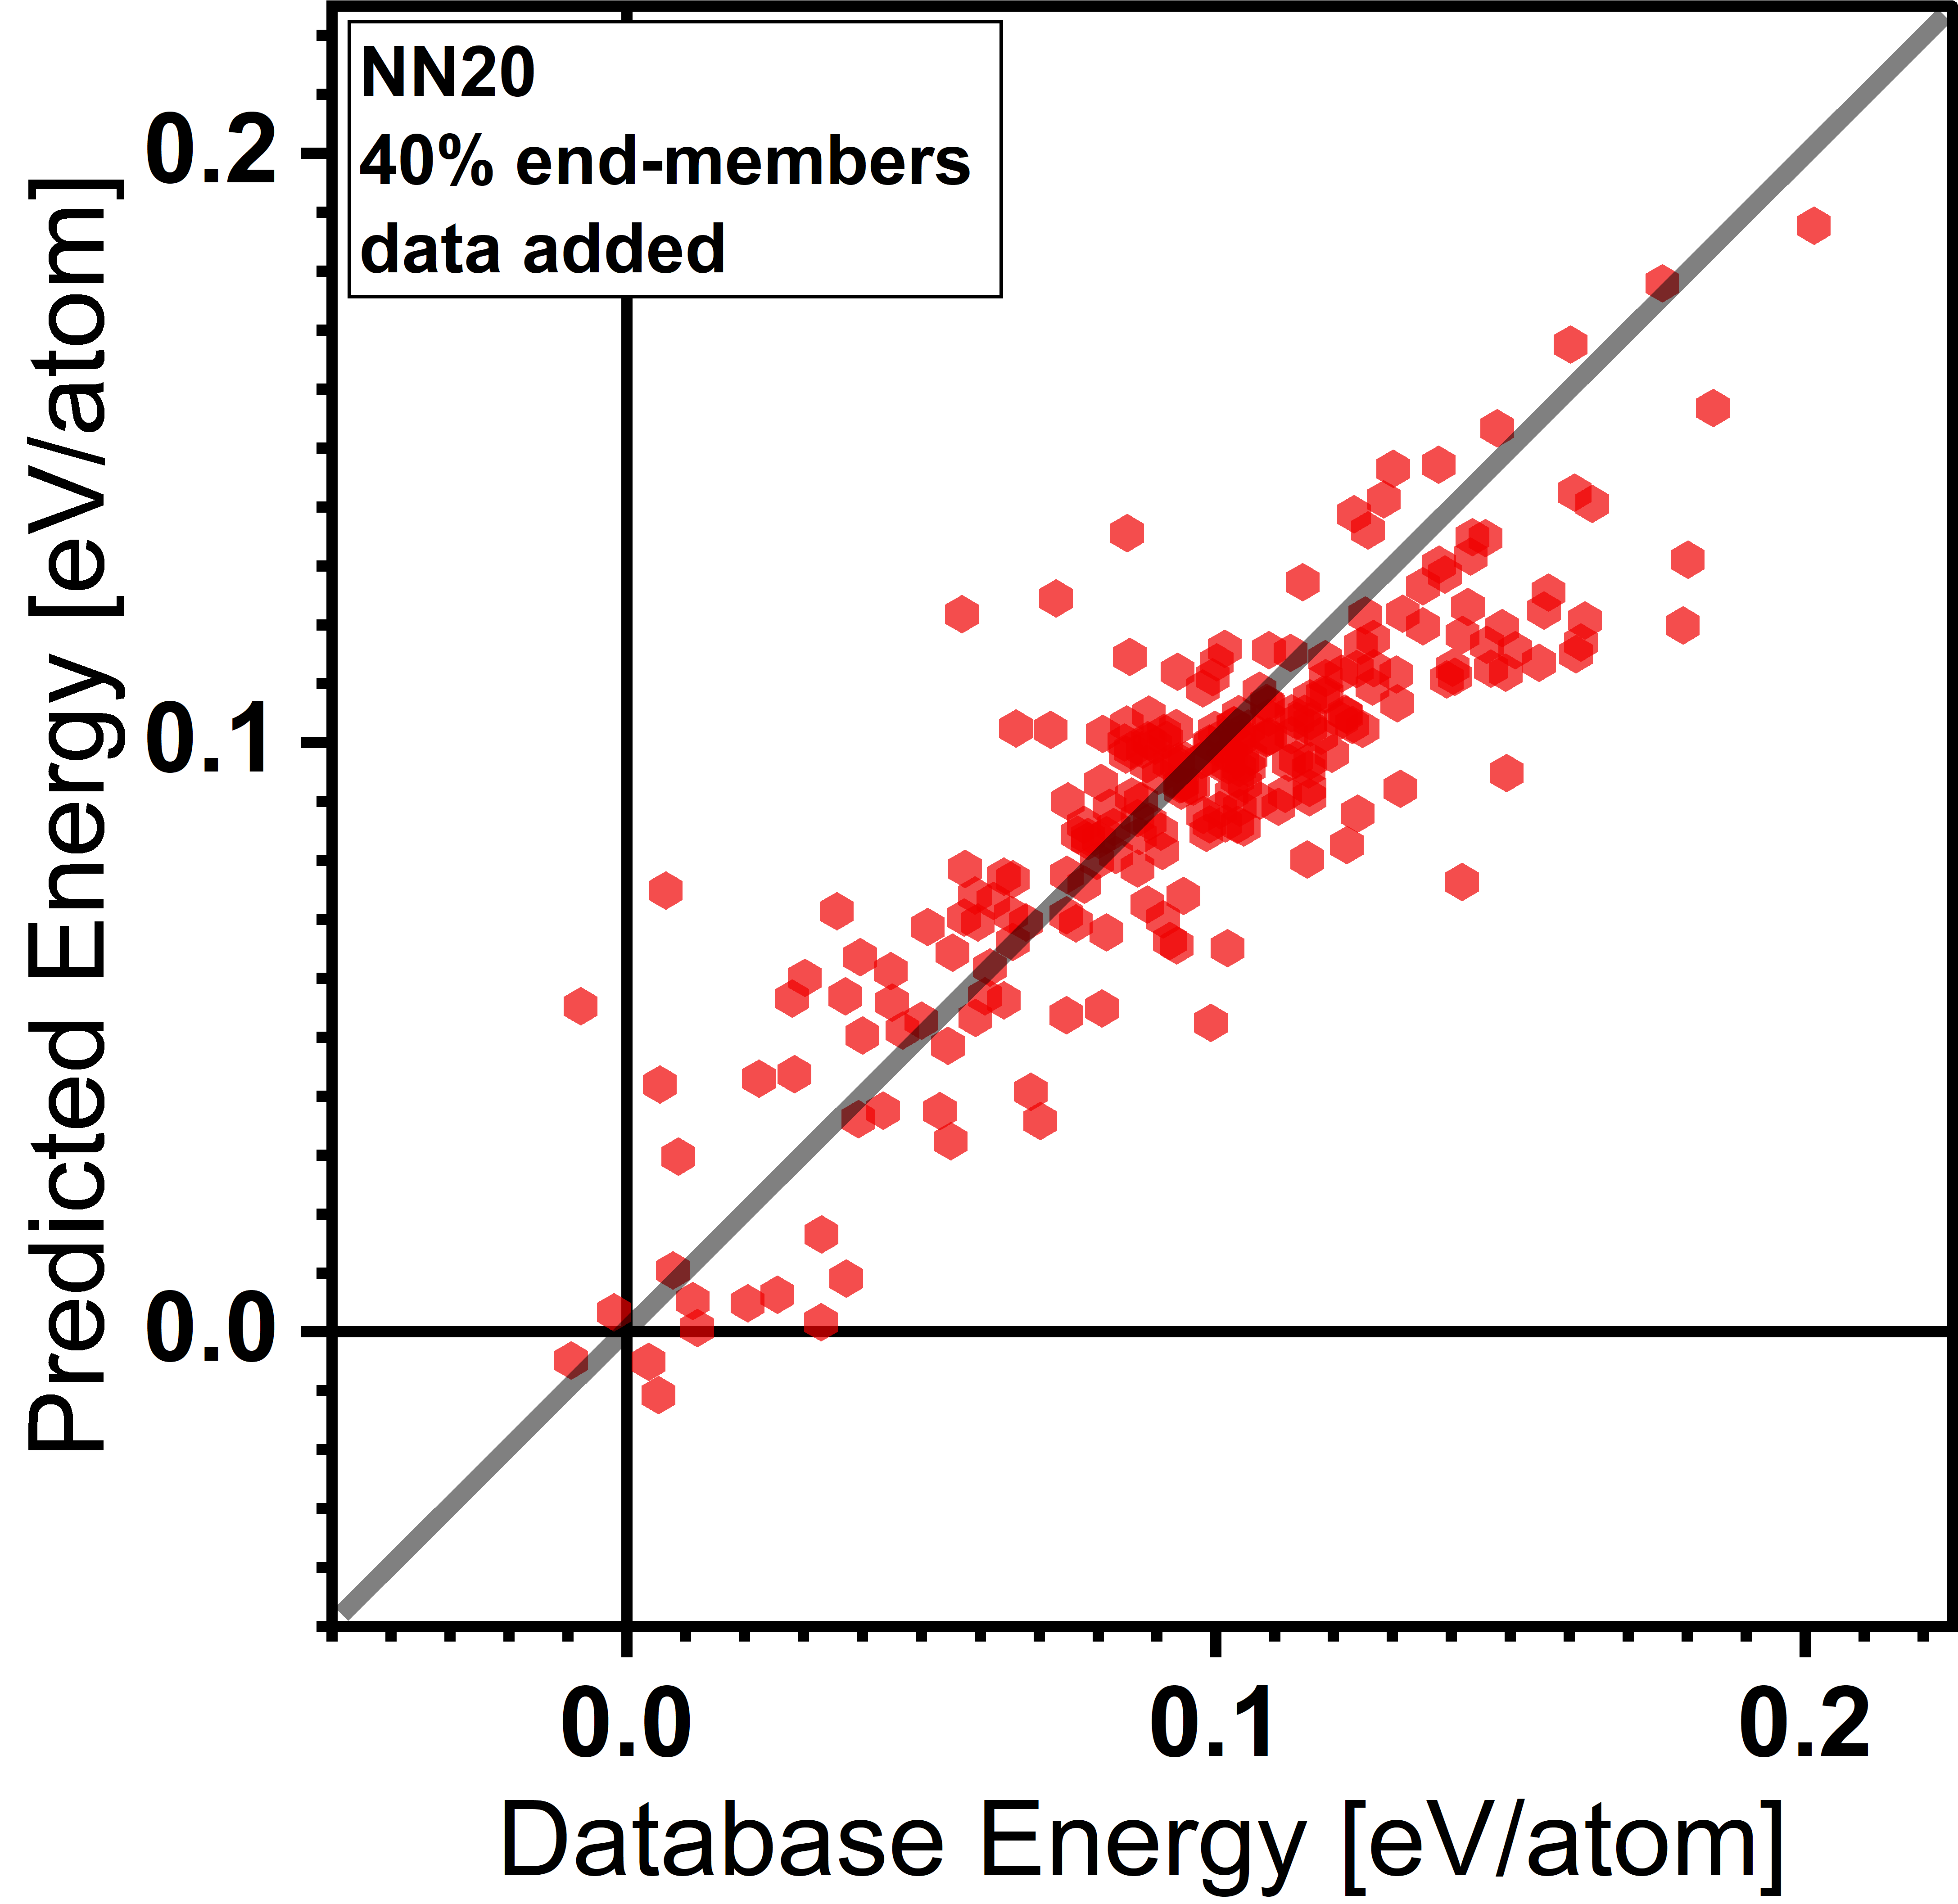
\includegraphics[width=0.24\textwidth]{sipfenn/NN20_SigmaTransfer_3.png}
    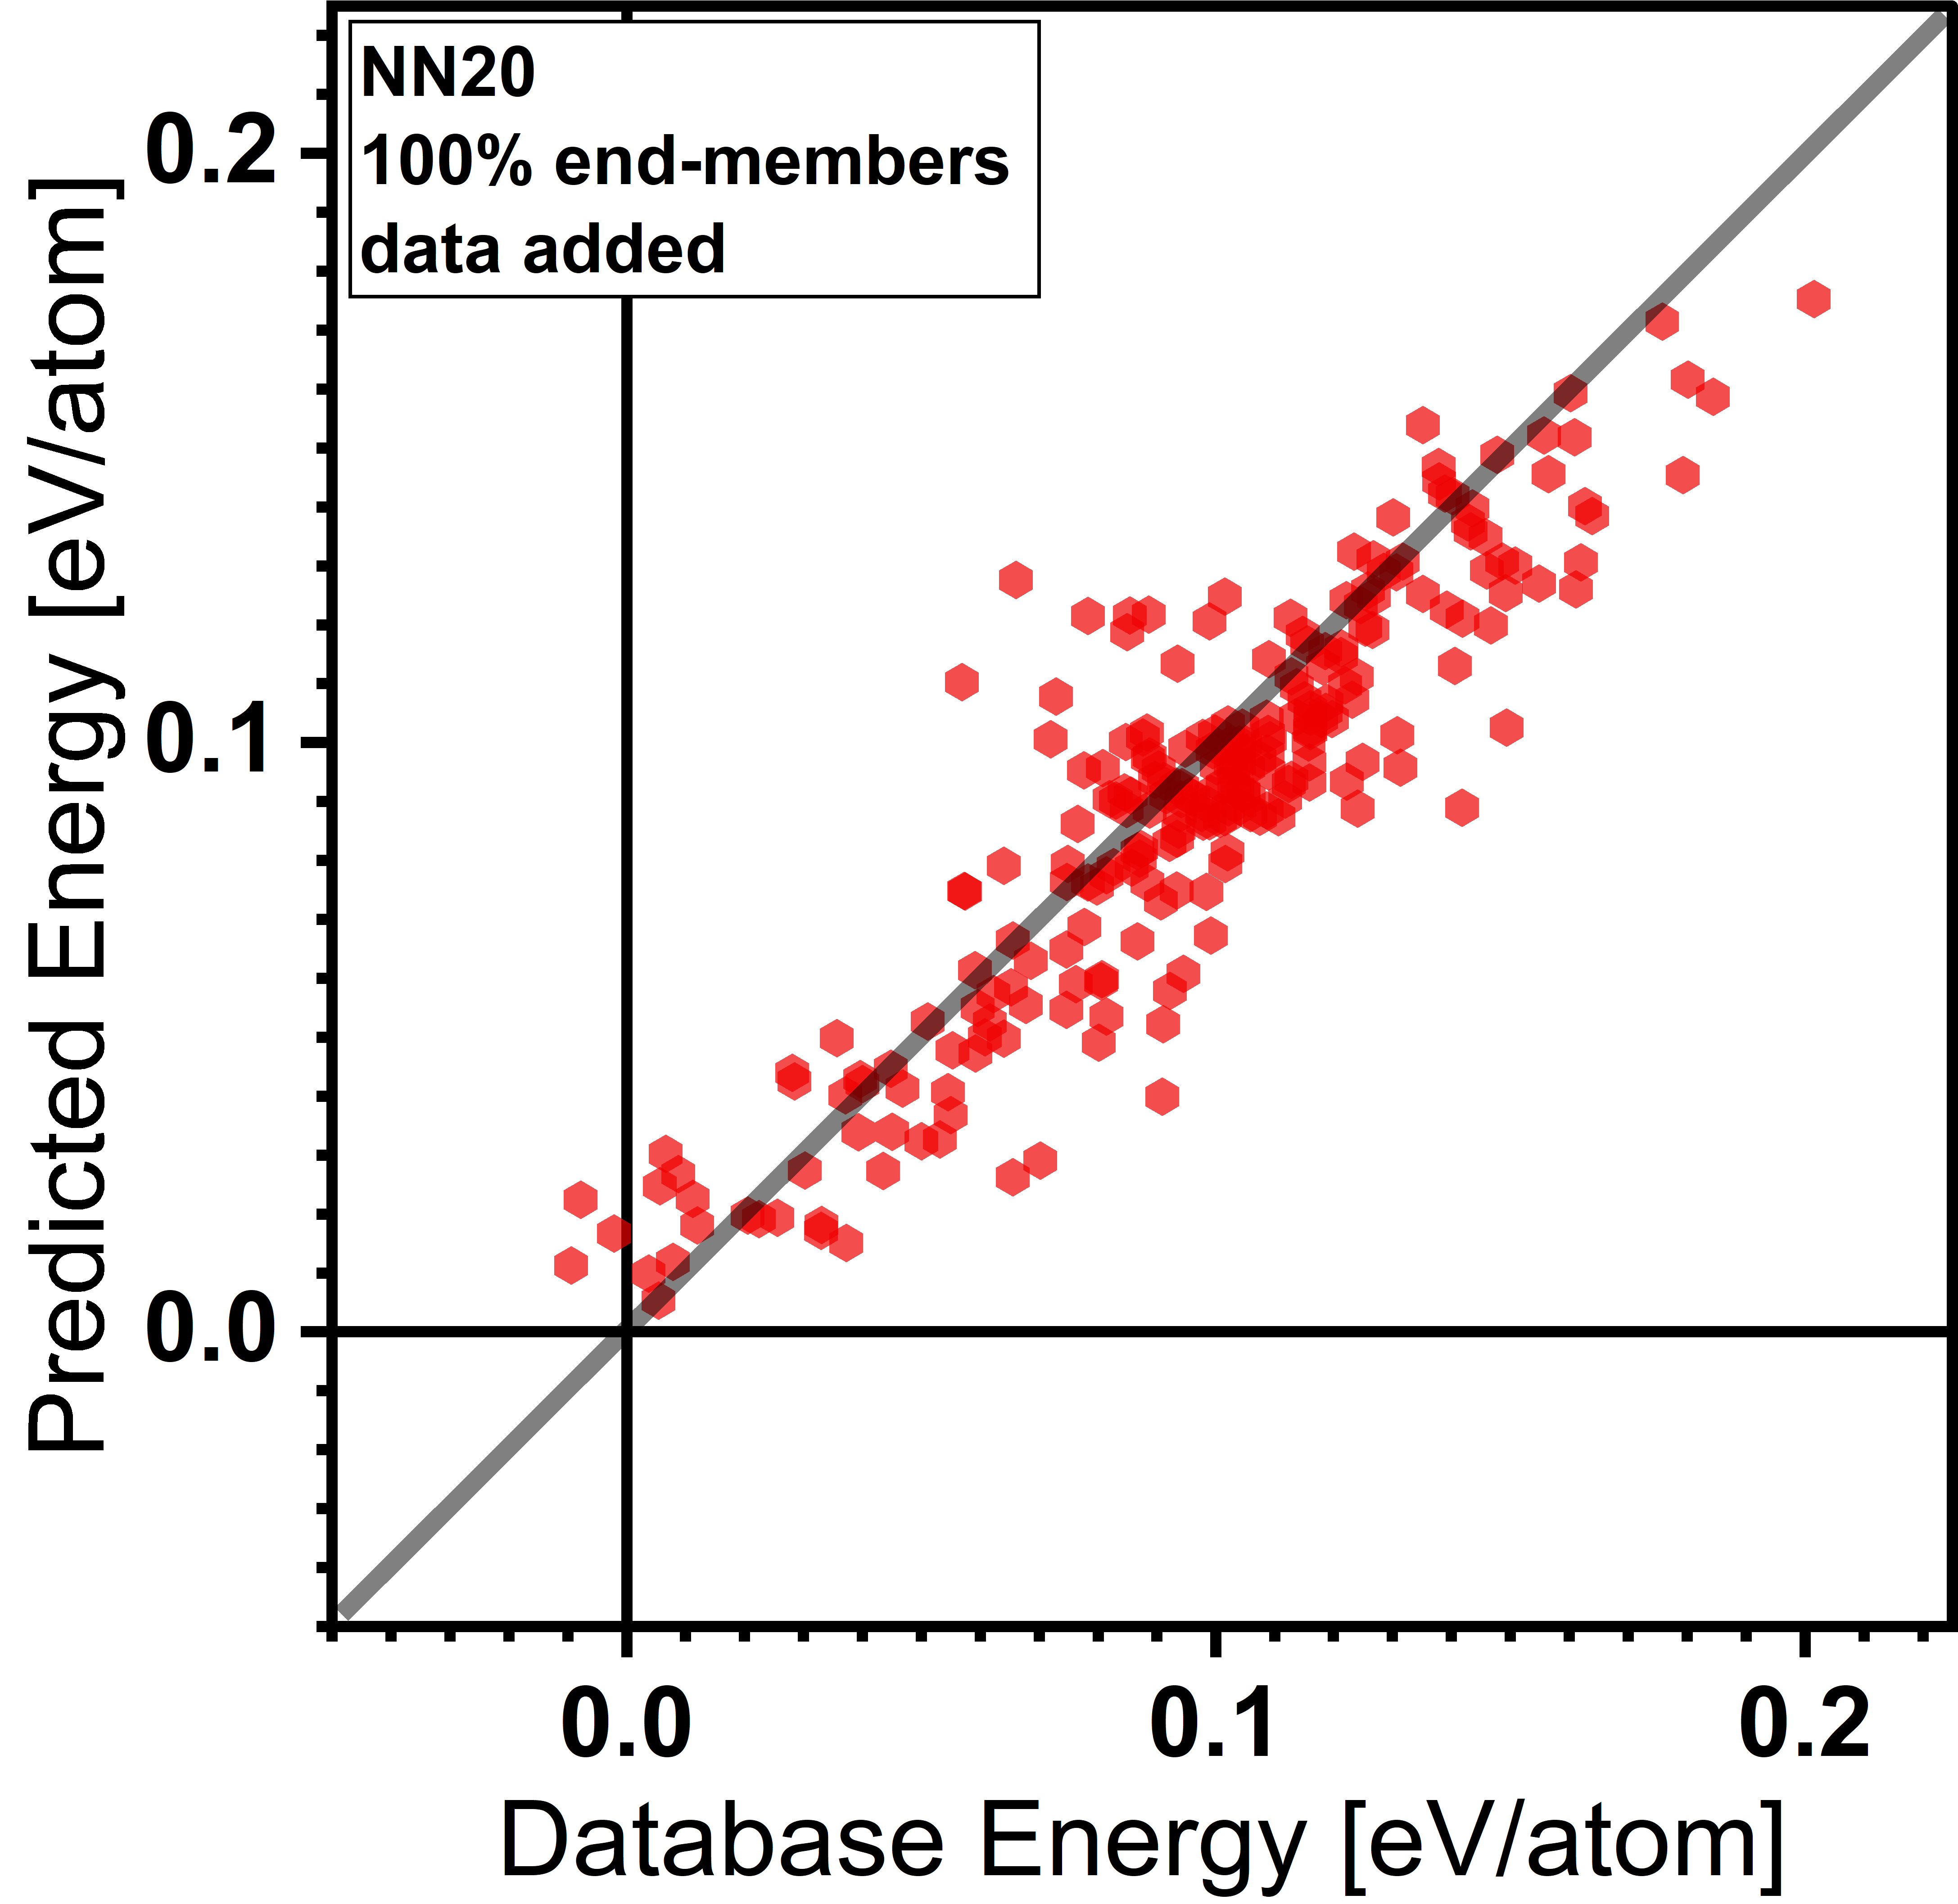
\includegraphics[width=0.24\textwidth]{sipfenn/NN20_SigmaTransfer_5.png}
    \caption{Performance of a new-materials-optimized network (NN20) on $\sigma$-phase data. Left-to-right: as trained on the OQMD, with additional training on 10\%, 40\%, and 100\% of the Fe-Cr-Ni $\sigma-$phase end-member data. The points on the figure correspond to all end-members (both training and testing data). Corresponding MAE and R are presented in Figure \ref{sipfenn:fig:transfersigmaARR} (gray rhombus points).}
    \vspace{-12pt}
    \label{sipfenn:fig:transfersigma}
\end{figure}


As depicted, adding just 10\% of DFT-calculated data (24/243 endmembers) provided a significant improvement in the prediction quality over the system, including the other 90\%  was never shown to the model. This result indicates that the models in the present paper can be combined with partial data obtained through DFT calculations to create accurate predictive tools for a specific closed material system, such as sublattice endmembers, and potentially limit the number of calculations required within the study. This can then provide the ability to investigate broader material search spaces at a given computational cost.

Furthermore, the presented transfer learning capability could be used for a more broad materials exploration without a well-defined finite search space like the ternary Fe-Cr-Ni $\sigma-$phase. In such a case, it is better to evaluate and report the performance of the model on a test set that wasn't presented during the training and report, as a function of the number of added data points (new DFT calculations). With such a problem statement, the transfer learning process has been repeated 1180 for the statistical significance of the outcomes, which are presented in Figure \ref{sipfenn:fig:transfersigmaVsDatapoints}.

\begin{figure}[H]
    \centering
    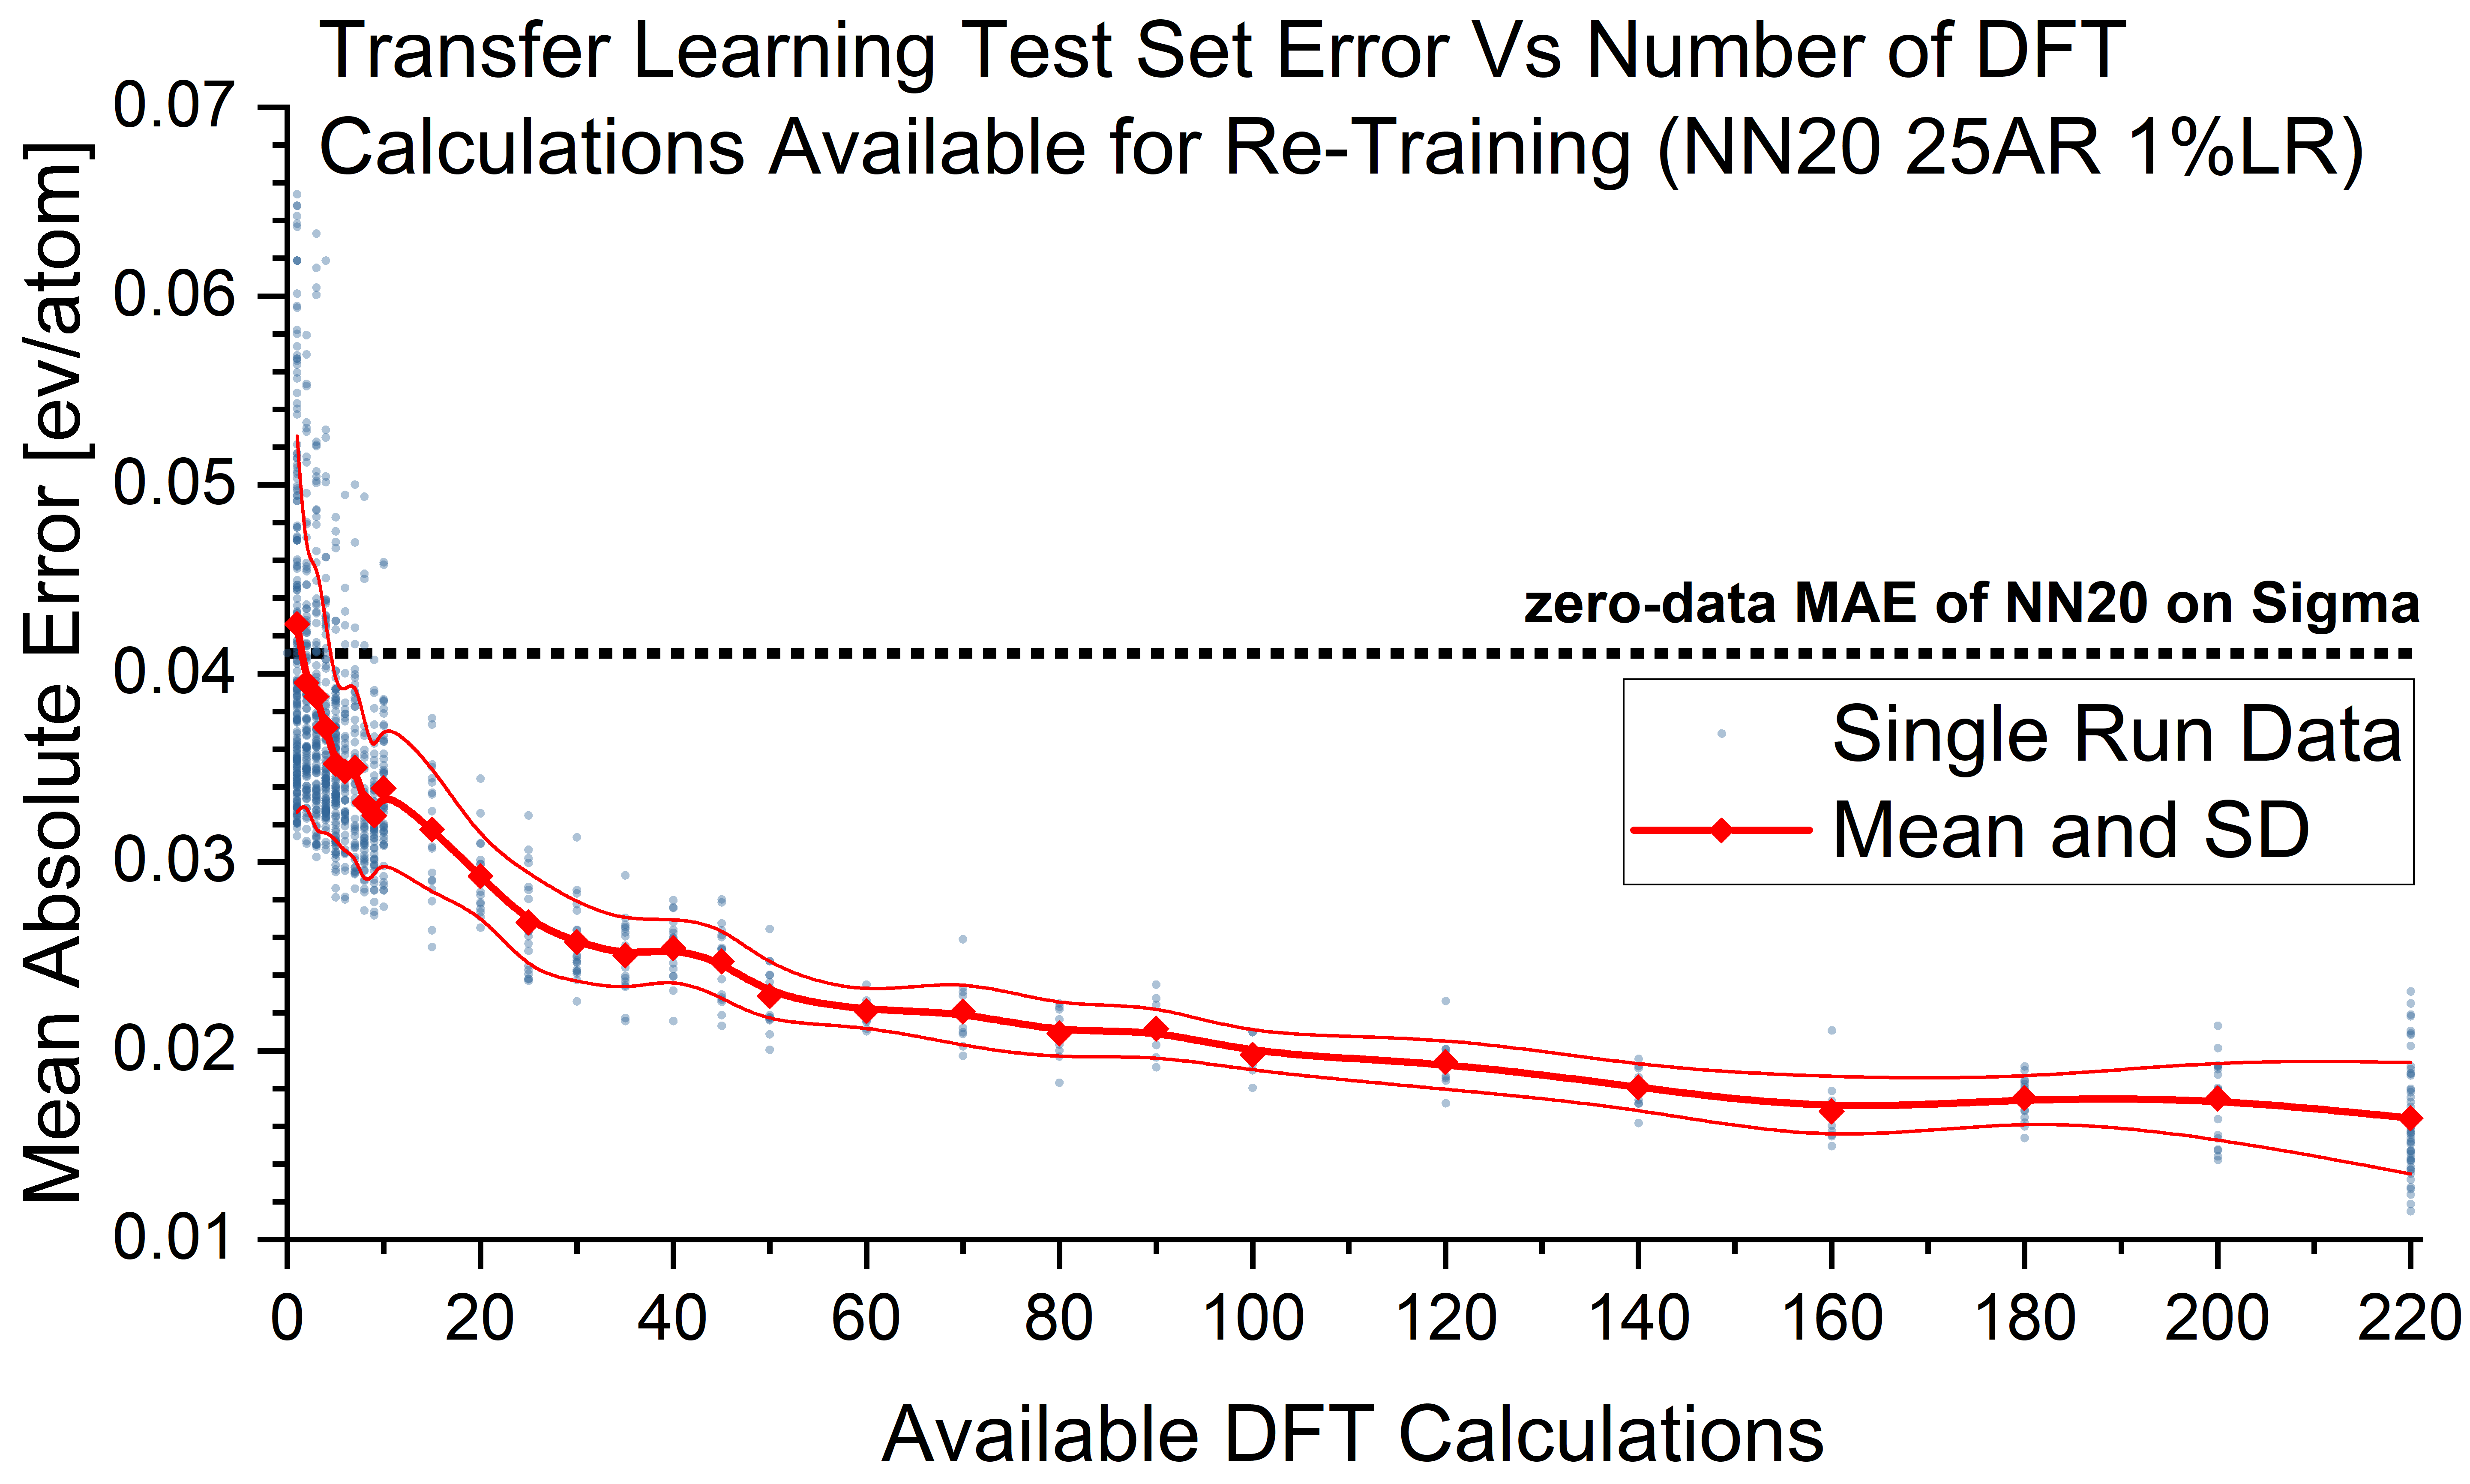
\includegraphics[width=0.48\textwidth]{sipfenn/transferLearning_vs_datapoints.png}
    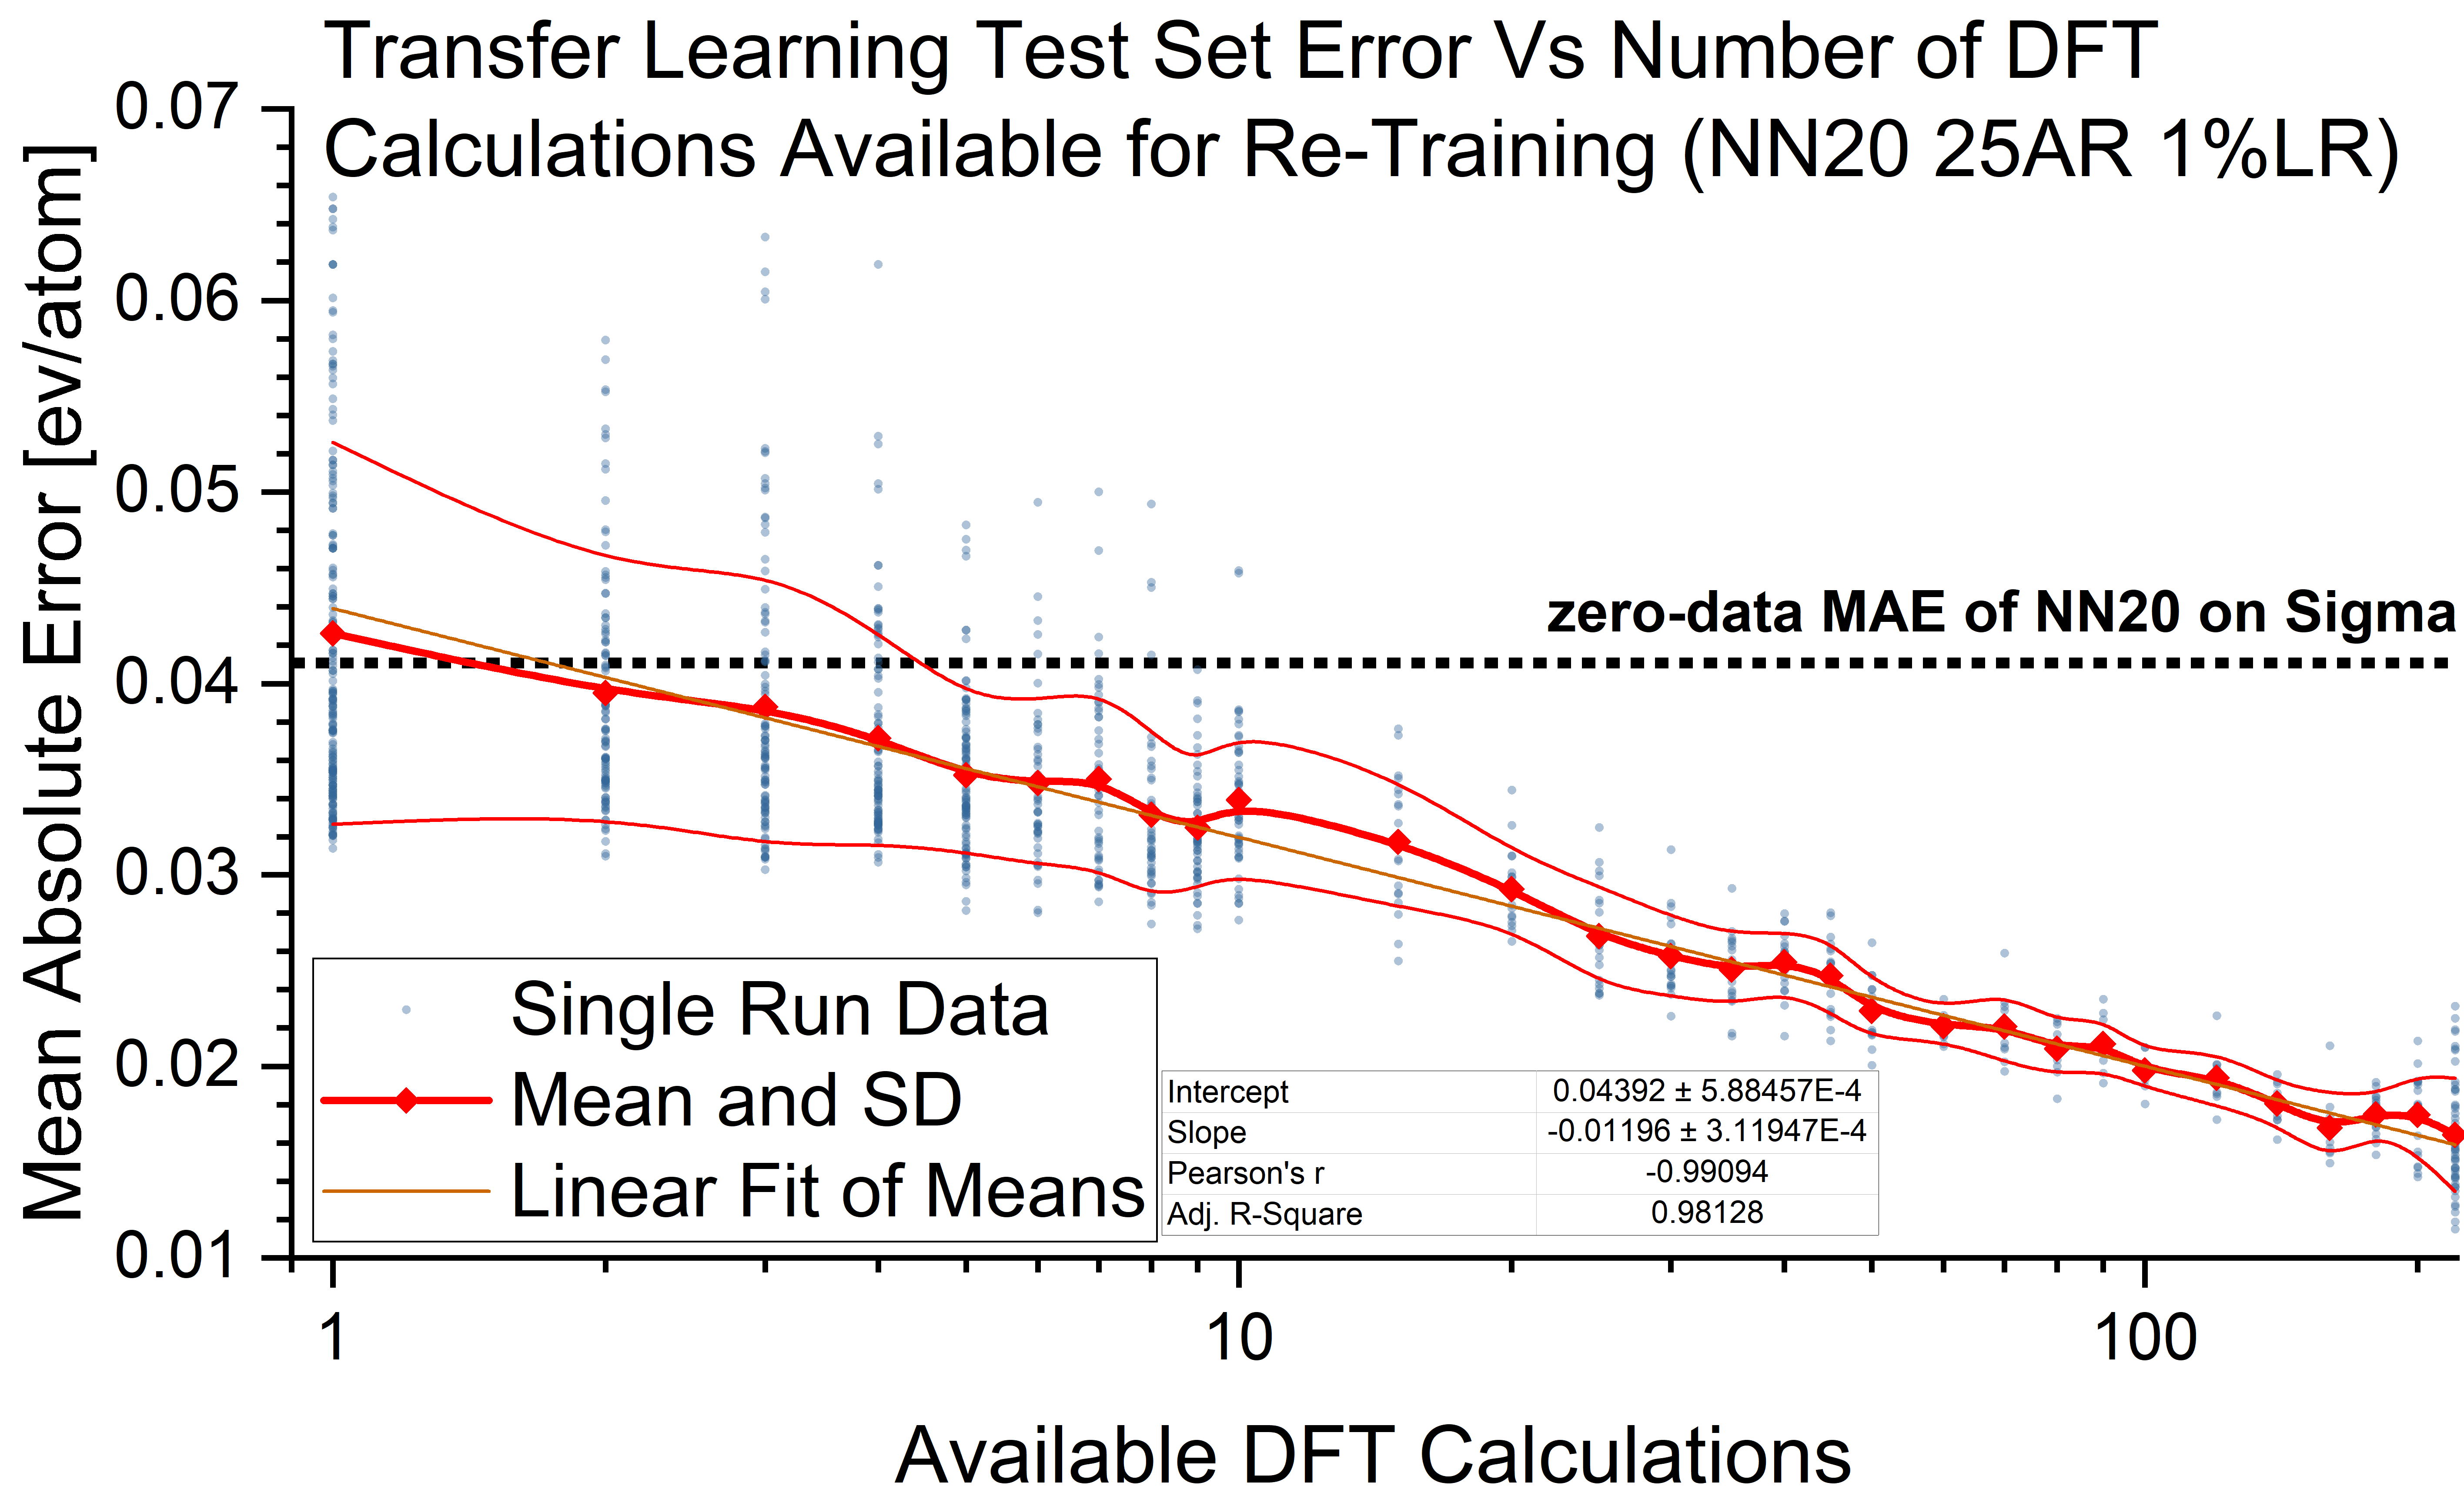
\includegraphics[width=0.48\textwidth]{sipfenn/transferLearning_vs_datapoints_LinLog.png}
    \caption{MAE of predictions evaluated on test set data vs number of newly available training datapoints. 1180 blue points correspond to single transfer learning processes. Red plot gives mean MAE and standard deviation. Both plots contain the same data.}
    \label{sipfenn:fig:transfersigmaVsDatapoints}
    \vspace{-12pt}
\end{figure}

As presented in Figure \ref{sipfenn:fig:transfersigmaVsDatapoints}, adding just a small number of new data points allows to nearly half the MAE (around 20 datapoints). Furthermore, evident from the right plot, the mean performance increase is on average linear in log-lin scale and highly predictable ($R^2=0.98$).

\subsection{Model Limitations} \label{sipfenn:ssec:modellimitations}
As with any modeling tool, this modeling effort has some inherent limitations, coning from both data and methods used to create it. The most significant one comes from the type of data used for training of the model, where all data points correspond to DFT-relaxed structures, sitting in local minima in the configuration energy landscape. Thus, all energy predictions are given under an assumption that the input structure is fully relaxed with DFT settings inherited from the OQMD database \cite{Saal2013MaterialsOQMD}. At the same time, since the model was trained on many local energy minima configurations analyzed on the level of single-atom chemical environments, it should be able to approximate values for unrelaxed structures based on substitution from prototypes or similar compounds. Testing of this is performed by Ward 2017 \cite{Ward2017IncludingTessellations}, where it is shown that (a) in most of the test cases, the before-after relaxation energy difference is negligible in comparison to the DFT-ML difference for Ward 2017 model and usually much lower than the test MAE for models discussed in this work, and (b) in some particular cases ($Li_6CaCeO_6$) can be very high.

When faced with a new configuration, the model can thus either be used to (1) give an accurate prediction if the configuration is already relaxed or (2) give an approximate result that needs to be validated with DFT if confidence in the result is needed. This is inherent to all structure-informed ML models. One possible solution to partially mitigate this limitation is to perform relaxation using the model, which should work reasonably well for most materials. 

Discussion of such relaxation procedure in detail is extensive and beyond the scope of this work, yet a preliminary approach was constructed using the Novel Material Model (NN2) and deployed on all 16 end-members of Pd-Zn $\gamma$-brass crystal structure \cite{Dasgupta2022} in an iterative fashion. At each iteration, first, the local energy gradient for each atom was calculated by comparing the starting configuration with perturbations in x, y, z directions. Then, all atoms were displaced proportionally to the gradient in 100 discrete steps, reaching some local minimum, which acted as a starting point for the next iteration. An example for $Pd_8Zn_5$ is presented in Figure \ref{sipfenn:fig:localrelaxationpdzn}.

\begin{figure}[H]
    \centering
    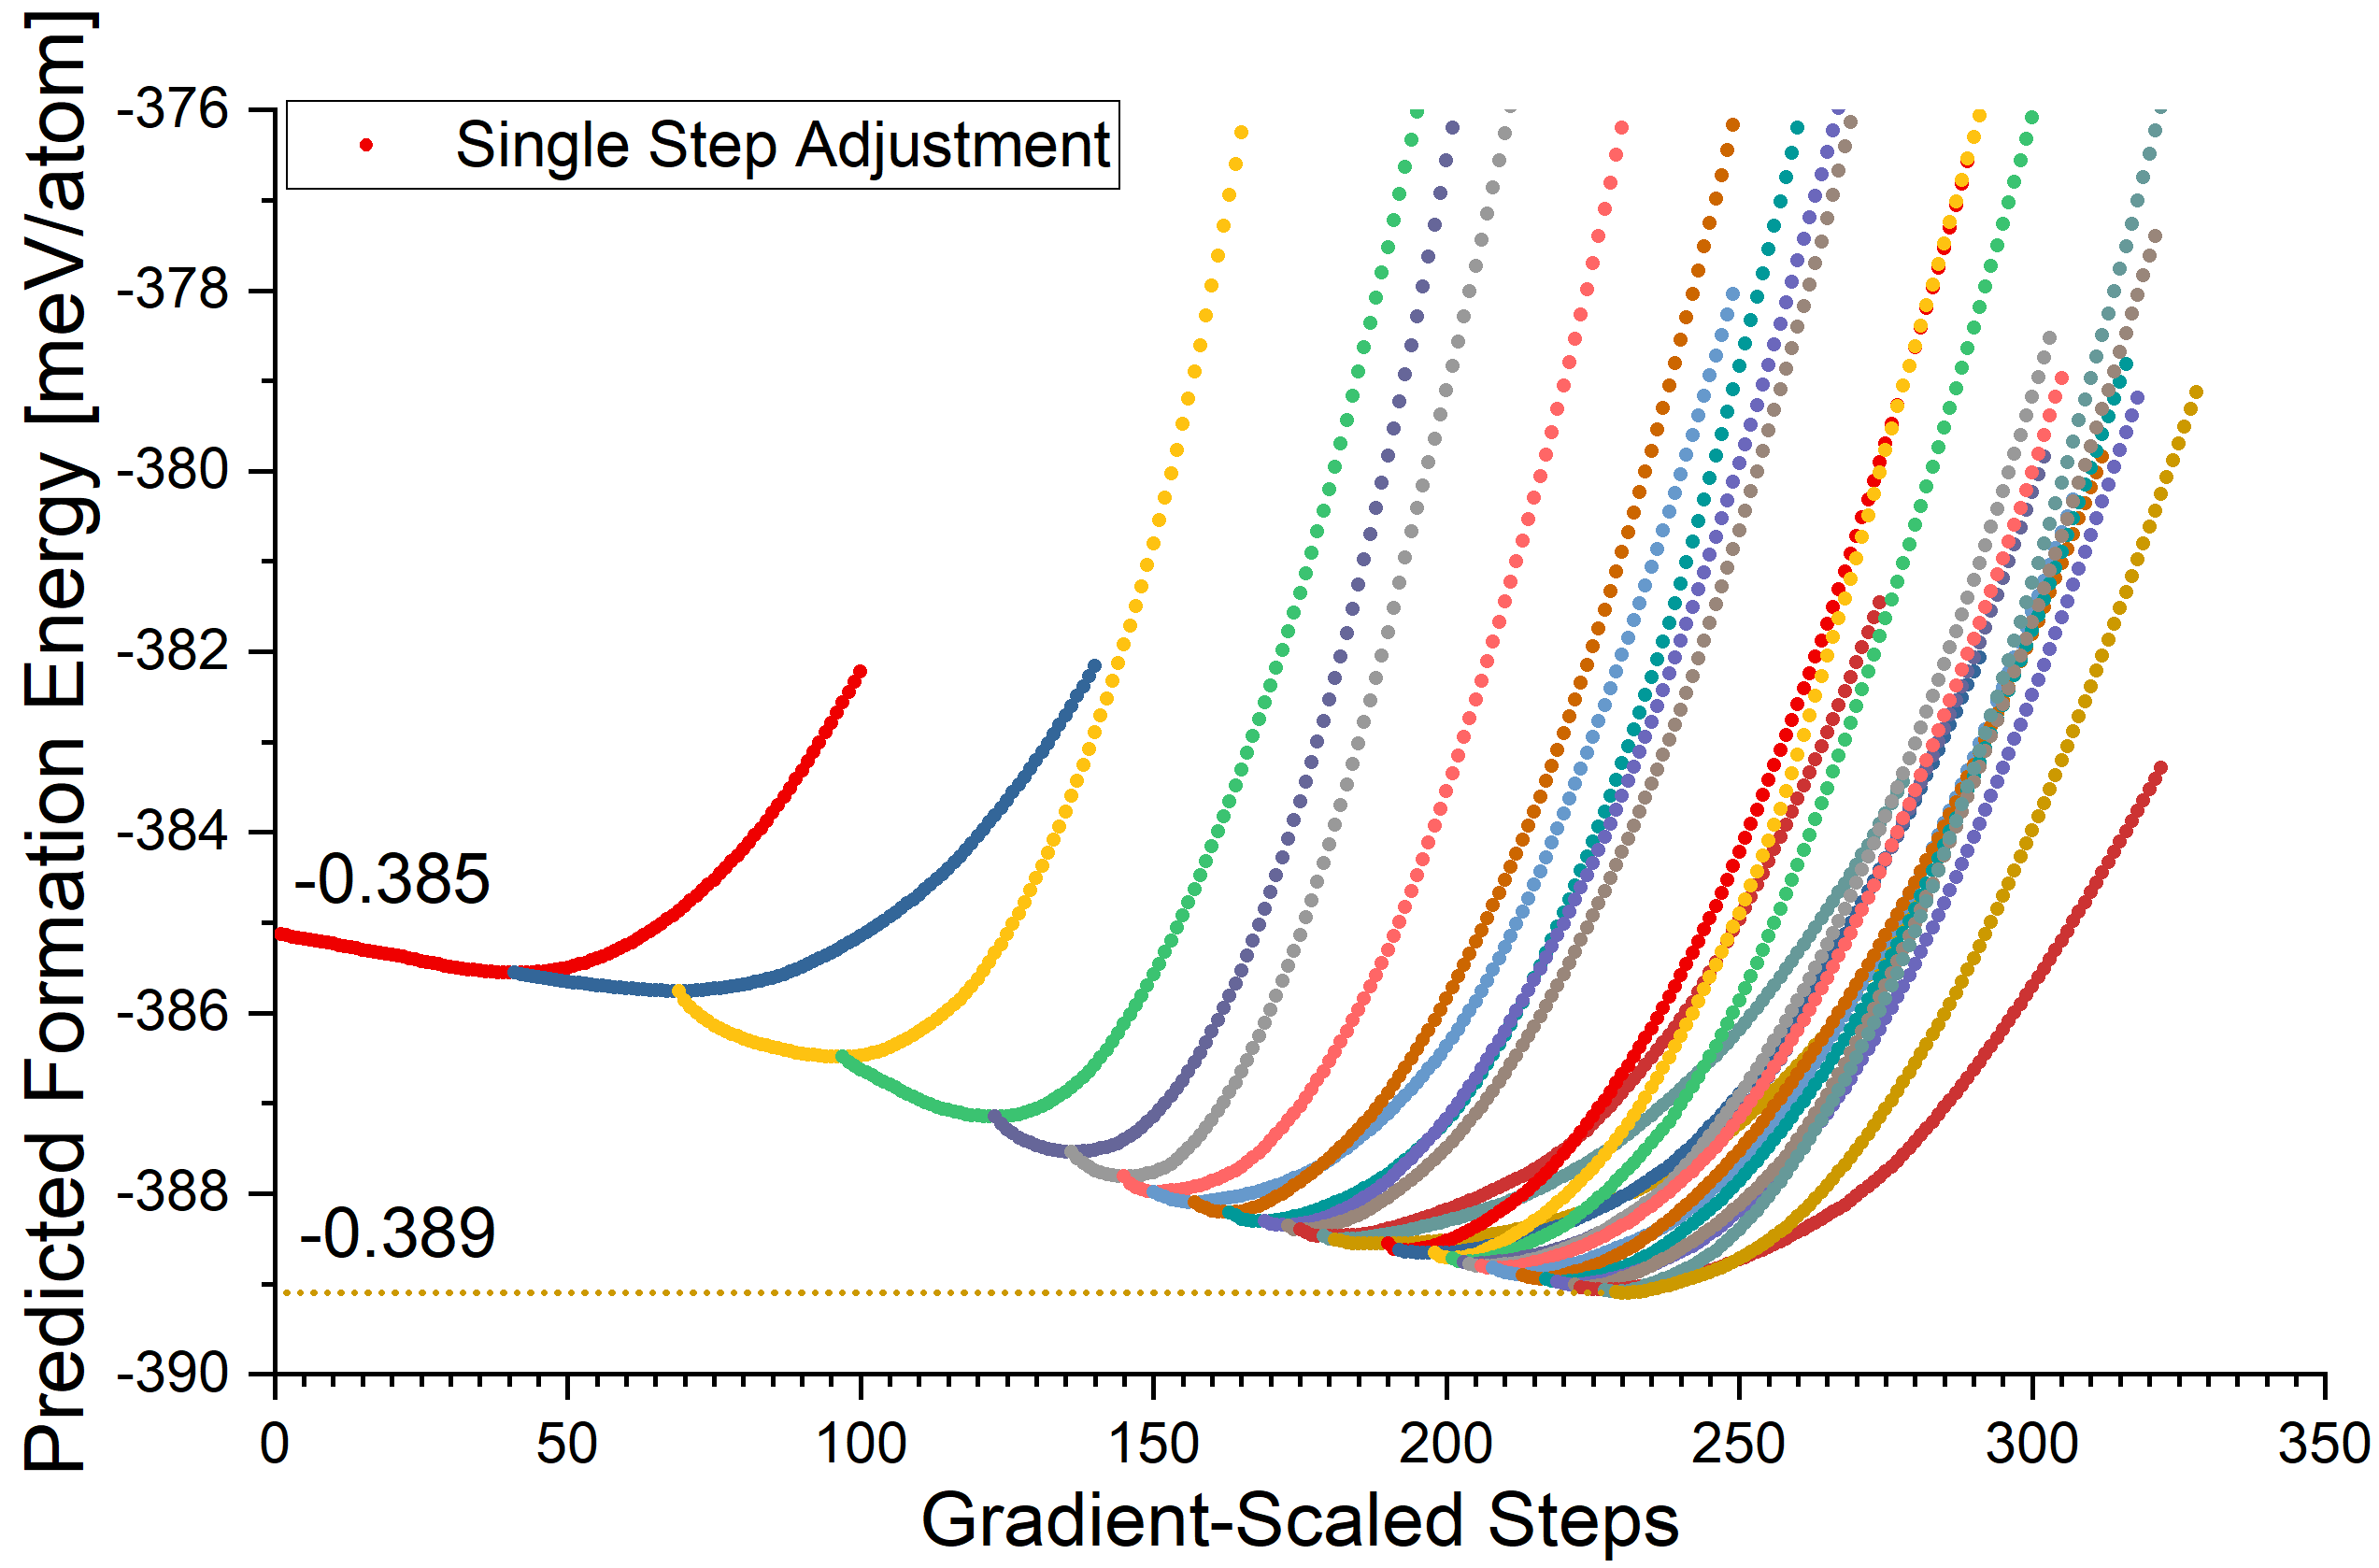
\includegraphics[width=0.7\textwidth]{sipfenn/localRelaxation_6.png}
    \caption{Local energy relaxation landscape of $Pd_8Zn_5$ $\gamma$-brass crystal structure from ideal positions guided iteratively by Novel Material Model (NN20).}
    \label{sipfenn:fig:localrelaxationpdzn}
\end{figure}

As shown in \ref{sipfenn:fig:localrelaxationpdzn}, the resulting relaxation reduced predicted formation energy by 4 meV/atom for this particular end-member. In the other 15 cases, results were similar, ranging between near 0 and 15 meV/atom, converging into fine local minima, expected to correspond with true local relaxations; however, extensive research into the problem is needed before conclusions can be drawn.


\subsection{End-User Implementation - SIPFENN} \label{sipfenn:ssec:SIPFENN}

One of the main objectives of the present paper was to create a tool that is transparent, easy to use by the research community, and easily modifiable. This lead to the creation of \texttt{SIPFENN} (Structure-Informed Prediction of Formation Energy using Neural Networks) software. \texttt{SIPFENN} provides the user with near-instant access to the models presented in \ref{sipfenn:sssec:DesignedModels}. In the future, this selection will likely be further expanded. On the user side, the use of the software is as easy as selecting one of the models, specifying a folder containing structure information files like \texttt{POSCAR}s \cite{POSCARFile} or \texttt{CIF}s \cite{Hall1991TheCrystallography}, running the predictions, and saving results.

\begin{figure}[H]
    \centering
    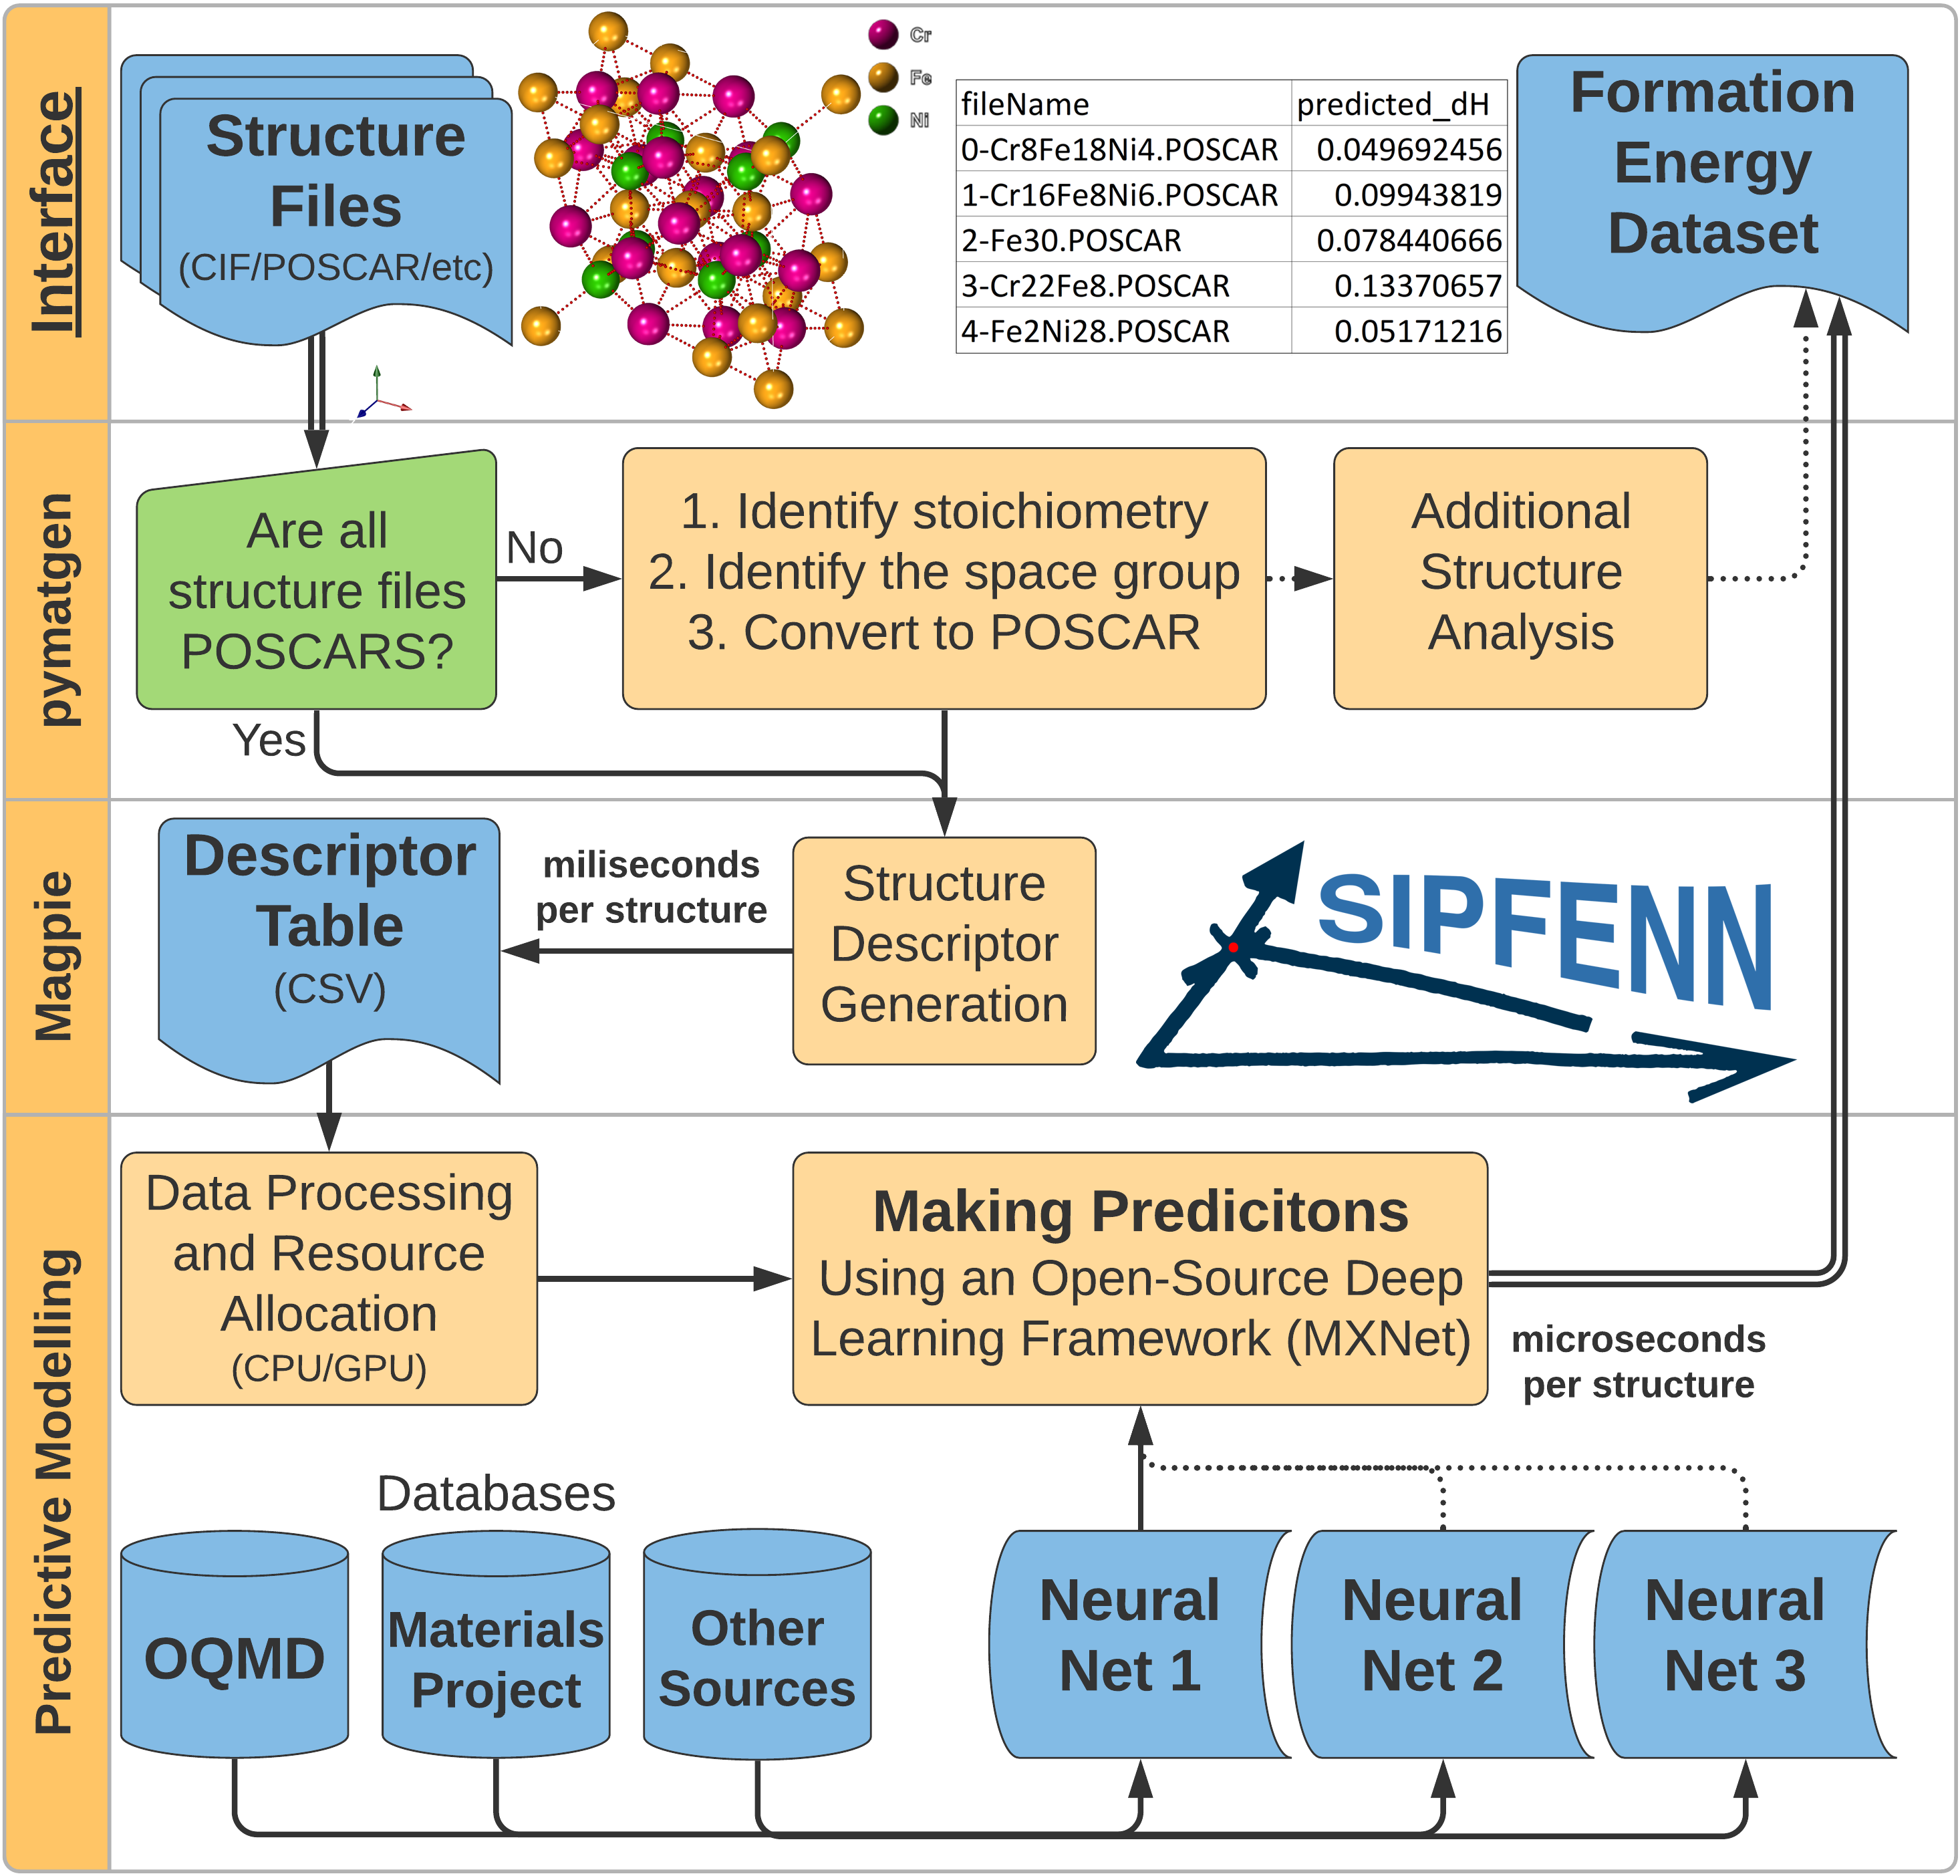
\includegraphics[width=0.67\textwidth]{sipfenn/SIPFENN_GraphicalAbstract_noPerformance.png}
    \caption{SIPFENN schematic description of operation.}
    \label{sipfenn:fig:sipfenn}
\end{figure}

SIPFENN was written entirely in Python to allow other researchers to easily modify it and adjust it to specific needs. Its schematic of operation is presented in Figure \ref{sipfenn:fig:sipfenn}. In broad scope, it first performs the structure analysis and modifications using the Python Materials Genomics library (\texttt{pymatgen}) \cite{Ong2013PythonAnalysis}. In the current implementation, it imports all structure files, analyzes the stoichiometry, creates unique names based on that, and exports them as POSCAR files. This is a rather simple task, however pymatgen is a powerful tool with a suit of more complex analytical tools that can be quickly implemented into \texttt{SIPFENN} by the user with even basic Python skills. Following the analysis, \texttt{SIPFENN} runs java-based Magpie \cite{Ward2016AMaterials} which calculates a descriptor for every imported structure and exports the result as a CSV file. This file is a descriptor table, where each row corresponds to a single material, and which can be stored and re-used later to run multiple predictive models at a fraction of the original computation time. It can also be used to create datasets for training procedures by replacing the last column with calculated or experimental values of formation energy.

Finally, the descriptor table is imported into the \texttt{MXNet} library framework, allocated into the CPU or GPU memory based on user selection, and evaluated using the selected predictive model. Once results are obtained, they are exported in CSV format and can be analyzed by any spreadsheet software such as Microsoft Excel.

\begin{figure}[H]
    \centering
    \frame{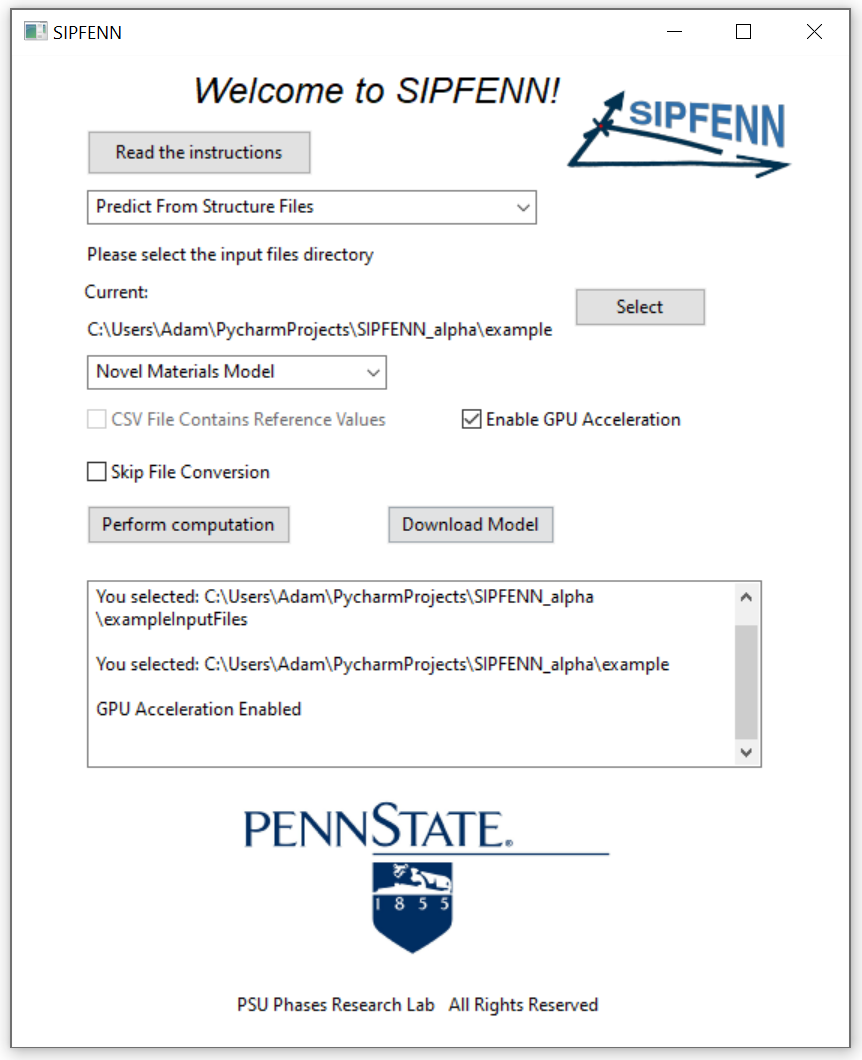
\includegraphics[width=0.55\textwidth]{sipfenn/sipfennGUI.PNG}}
    \caption{A snapshot of the graphical user interface of SIPFENN.}
    \label{sipfenn:fig:sipfennGUI}
\end{figure}

\texttt{SIPFENN} was planned as a command-line tool, however, it was recognized that some users, especially those with little computational background, may find that difficult. Therefore, a simple graphical user interface (GUI) was created using \texttt{wxPython} library. It incorporates all the capabilities of the command line version. Furthermore, it lets the user download the predictive models from a repository in a single click. A sample snapshot of the GUI before performing calculations is presented in Figure \ref{sipfenn:fig:sipfennGUI}.

\section{Conclusions} \label{sipfenn:ssec:Conclusions}
In the present paper new machine learning models and a ready-to-use tool were created, based on the dataset and descriptor design by Ward et al. \cite{Ward2017IncludingTessellations}. Models reported in this work significantly improve upon existing methods, both in terms of performance and accessibility. For the most direct comparison, one of the designed models has been optimized for performing well on a random subset of the OQMD database and achieved an MAE of 28 meV/atom, compared to 80 meV/atom in the original  Ward et al. paper \cite{Ward2017IncludingTessellations}, and to 38 meV/atom in the most recent model called \texttt{IRNet} \cite{Jha2019IRNet}. Furthermore, it was shown that the error of the model is lowered when applied to the problem of finding the convex hull energy, achieving levels comparable with the current state-of-the-art approaches \cite{Jha2018ElemNet:Composition, Goodall2020PredictingStoichiometry}.

In addition, using appropriate overfitting mitigation efforts, such as Dropout and L2 regularization, models tuned for generalization to other types of materials datasets were developed. To test this, the models were evaluated on two datasets not contained within the OQMD, namely all end-members (243) of 5-sublattice topologically-close-packed Fe-Cr-Ni Sigma-phase \cite{Feurer2019Cr-Fe-NiCalculations, Hsieh2012OverviewSteels} and a few selected random-solution-approximating SQS \cite{Zunger1990SpecialStructures, Shin2006ThermodynamicStructures, Jiang2004First-principlesStructures}. The MAE values for these two test sets were found to be close to the values obtained on a test set from the OQMD. This exemplifies that the models are able to generalize to new datasets.
%In total, over 50 neural networks were trained on the dataset of around 400,000 DFT calculation results contained within the OQMD database\cite{Saal2013MaterialsOQMD, Kirklin2015TheEnergies}. This process lead to three final neural networks specialized in defined objectives, including the state-of-the-art performance on the random subset of OQMD, with mean absolute error (MAE) of 28 meV/atom. The second and most advanced neural network was optimized for predicting new materials, and consequently its usability in new materials discovery.
% The second network provides MAE of 42 meV/atom, which still constitutes a significant improvement over previous tools, but has reduced size, allowing the network to run on low power devices such as smartphones. 

Furthermore, it was shown that models created within the present paper can be used for transfer learning, where vast knowledge of a broad spectrum of materials is combined with as little as a few DFT-datapoints from a specific materials system to provide excellent results within that specific system. Such at least partially process mitigates the issue of low data availability, present in numerous materials science problems, and consequently allows users to investigate a broader scope of materials at the same computational cost.

Finally, the three neural network models designed within the present paper were used, in conjunction with additional software, to create an end-user tool called \texttt{SIPFENN}. \texttt{SIPFENN}'s capabilities extend far beyond allowing validation of the presented results. It is implemented to work without any intensive computations on the user side, using models accessible from a repository, requiring only a quick one-click model download  to run. It is very fast thanks to using one of the industry's leading ML frameworks capable of well-optimized computations on GPUs. Furthermore, it is an open-source tool written in \texttt{Python}, which can be easily modified to specific needs in a straightforward way without extensive changes in the code.


\section{Software and Data Availability}

As of 2022, the \texttt{SIPFENN} code has been deprecated in favor of highly improved \texttt{pySIPFENN} which was re-written with great stability, reliability, and deeper integration with other community tools. Chapter \ref{chap:pysipfenn} describes it in detail and Section \ref{pysipfenn:sec:softwareavaialbility} describes its availability along related workshops and tutorial materials.

For archival purposes, the last version of \texttt{SIPFENN} code is available through Penn State's Phases Research Lab website at 
\href{https://phaseslab.org/sipfenn}{https://phaseslab.org/sipfenn} in (1) a minimal version that can be run on pre-computed descriptors in CSV format as well as (2) ready-to-use version with pre-compiled Magpie \cite{Ward2016AMaterials}. \texttt{SIPFENN} contains hard-coded links to neural networks stored in the cloud that can be downloaded at a single-click (see Figure \ref{sipfenn:fig:sipfennGUI}). 

All neural networks were made available in (1) open-source \texttt{MXNet} format maintained by Apache Foundation, used within \texttt{SIPFENN}, (2) closed-source \texttt{WLNet} format maintained by Wolfram Research and having the advantage of even easier deployment, as well as guaranteed forward compatibility with future versions of Wolfram Language, and in (3) Open Neural Network Exchange (\texttt{ONNX}) format \cite{Bai2019ONNX:Exchange} distributed through \texttt{pySIPFENN}, as of April 2024.

For ensured longevity of results, original \texttt{SIPFENN} neural networks are stored through the courtesy of Zenodo.org service under DOI:~\href{https://doi.org/10.5281/zenodo.4006803}{10.5281/zenodo.4006803} at the CERN’s Data Centre.

\pagebreak


\printbibliography[heading=subbibintoc]


\chapter{Efficient Structure-Informed Featurization} \label{chap:pysipfenn}

Structure-informed materials informatics is a rapidly evolving discipline of materials science relying on the featurization of atomic structures or configurations to construct vector, voxel, graph, graphlet, and other representations useful for machine learning prediction of properties, fingerprinting, and generative design. This work discusses how current featurizers typically perform redundant calculations and how their efficiency could be improved by considering (1) fundamentals of crystallographic (orbits) equivalency to optimize ordered cases and (2) representation-dependent equivalency to optimize cases of dilute, doped, and defect structures with broken symmetry. It also discusses and contrasts ways of (3) approximating random solid solutions occupying arbitrary lattices under such representations.

Efficiency improvements discussed in this work were implemented within \texttt{pySIPFENN} or \textit{python toolset for Structure-Informed Property and Feature Engineering with Neural Networks} developed by authors since 2019 and shown to increase performance from 2 to 10 times for typical inputs. Throughout this work, the authors explicitly discuss how these advances can be applied to different kinds of similar tools in the community.

\section{Introduction} \label{pysipfenn:sec:Introduction}

\texttt{SIPFENN} or \textit{Structure-Informed Prediction of Formation Energy using Neural Networks} software, first introduced by the authors in 2020 \cite{Krajewski2022ExtensibleNetworks, Krajewski2020SIPFENNModels}, is one of several open-source tools available in the literature \cite{Ward2017, Jha2019IRNet, Chen2019GraphCrystals, Choudhary2021AtomisticPredictions, Deng2023CHGNetModelling, Davariashtiyani2023FormationRepresentation, Davariashtiyani2023FormationRepresentation, Schmidt2023Machine-Learning-AssistedMaterials} which train machine learning (ML) models on the data from large Density Functional Theory (DFT) based datasets like \texttt{OQMD} \cite{Saal2013MaterialsOQMD, Kirklin2015TheEnergies, Shen2022ReflectionsOQMD}, \texttt{AFLOW} \cite{Curtarolo2013AFLOW:Discovery, Toher2018TheDiscovery}, Materials Project \cite{Jain2013Commentary:Innovation}, NIST-\texttt{JARVIS}\cite{Choudhary2020TheDesign}, \texttt{Alexandria} \cite{Schmidt2022AFunctionals}, or \texttt{GNoME} \cite{Merchant2023ScalingDiscovery} to predict formation energies of arbitrary atomic structures, with accuracy high enough to act as a low-cost surrogate in the prediction of thermodynamic stability of ground and non-ground state configurations at 0K temperature. The low runtime cost allows such models to efficiently screen through millions of different atomic structures of interest on a personal machine in a reasonable time. 

In addition to high-accuracy neural network models trained on \texttt{OQMD} \cite{Saal2013MaterialsOQMD, Kirklin2015TheEnergies, Shen2022ReflectionsOQMD}, \texttt{SIPFENN} included a number of features not found in competing tools available at the time, such as the ability to quickly readjust models to a new chemical system based on just a few DFT data points through transfer learning and a selection of models optimized for different objectives like extrapolation to new materials instead of overfitting to high-data-density regions or low memory footprint \cite{Krajewski2022ExtensibleNetworks}.

\texttt{SIPFENN}'s usefulness has been demonstrated, for instance, in the cases where the structure of an experimentally observed compound could not be identified in industry-relevant Nd-Bi \cite{Im2022ThermodynamicModeling} and Al-Fe \cite{Shang2021FormingJoints} systems and had to be predicted. This was accomplished by (1) high-throughput generation of hundreds of thousands of possible candidates with the exact stoichiometry based on elemental substitutions into structures from both open DFT-based databases \cite{Saal2013MaterialsOQMD, Kirklin2015TheEnergies, Shen2022ReflectionsOQMD, Curtarolo2013AFLOW:Discovery, Toher2018TheDiscovery, Jain2013Commentary:Innovation, Choudhary2020TheDesign, Schmidt2022AFunctionals, Merchant2023ScalingDiscovery} and experimentally observed ones from Crystallography Open Database (COD) \cite{Grazulis2009CrystallographyStructures, Grazulis2012CrystallographyCollaboration, Grazulis2019CrystallographyPerspectives}, followed by (2) selection of thousands of low-energy candidates, (3) down-selection of tens of unique candidates based on clustering in the \texttt{SIPFENN}'s feature space, and (4) final validation with DFT and experiments. It has also been deployed in several thermodynamic modeling studies, e.g. of Nb-Ni system \cite{Sun2023ThermodynamicESPEI}, in conjunction with DFT and experimental data processed through \texttt{ESPEI} \cite{Bocklund2019ESPEICuMg} to automatically fit parameters of CALPHAD \cite{Olson2023GenomicDynamics} models deployed in \texttt{pycalphad} \cite{Otis2017Pycalphad:Python}.


\section{General Structure Featurization Improvements} \label{pysipfenn:sec:featurization}

\subsection{pySIPFENN Overview and Core Advantages} \label{pysipfenn:ssec:coreimprovements}

Being able to predict the thermodynamic stability of arbitrary atomic structures and their modifications is one of the most critical steps in establishing whether hypothetical candidates can be made in real life \cite{Zunger2019BewareMaterials}; however, it is certainly not the only task of interest to the community \cite{Jha2023MachineChallenges, Tao2021MachineDiscovery}. These diverse needs, combined with increasing interest in multi-property modeling, have shifted the focus of \texttt{SIPFENN} tool from model training \cite{Krajewski2022ExtensibleNetworks} toward the development of reliable, easy-to-use, and efficient general-purpose featurizers existing in a framework, which can be used by researchers and companies to quickly develop and deploy property-specific models, or use features directly in exploring similarity and trends in materials.

Thus, while the acronym has been retained, the name of the software has been changed to \textit{python toolset for Structure-Informed Property and Feature Engineering with Neural Networks} or \texttt{pySIPFENN}, and the software component has been carefully re-implemented in its entirety to make it as general as possible and enable the following core advantages:

\begin{enumerate}
    
    \item Reliable featurization, which can be immediately transferred to other tools thanks to standalone submodule implementations based only on two common libraries (\texttt{NumPy} \cite{Harris2020ArrayNumPy} and \texttt{pymatgen} \cite{Ong2013PythonAnalysis}). These include completely re-written \texttt{Ward2017} Java-based featurizer \cite{Ward2017} (see Section \ref{pysipfenn:ssec:Ward2017Translation}) and 3 new ones, described in Sections \ref{pysipfenn:sec:ordered}, \ref{pysipfenn:sec:dilute}, and \ref{pysipfenn:sec:randomsolutions}.

    \item Effortless plug-and-play deployment of neural network (and other) ML models (for any property) utilizing any of the defined feature vectors, enabled by the use of Open Neural Network Exchange (\texttt{ONNX}) open-source format \cite{Bai2019ONNX:Exchange} which can be exported from nearly every modern ML framework and is then loaded into \texttt{pySIPFENN}'s \texttt{PyTorch} backend \cite{Paszke2019PyTorch:Library} through \texttt{onnx2torch} \cite{Kalgin2021Onnx2torch:PyTorch}. Furthermore, implementing custom predictors, beyond those supported by \texttt{PyTorch}, is made easy by design.

    \item Dedicated \texttt{ModelExporters} submodule makes it easy to export trained models for publication or deployment on a different device while also enabling weight quantization and model graph optimizations to reduce memory requirements.

    \item The ability to acquire data and adjust or completely retrain model weights through automated \texttt{ModelAdjusters} submodule. Its applications include:
    \begin{enumerate}
        \item Fine-tuning models based on additional local data to facilitate transfer learning ML schemes of the domain adaptation kind \cite{Ben-David2010ADomains}, where a model can be adjusted to new chemistry and specific calculation settings, introduced by \texttt{SIPFENN} back in 2020 \cite{Krajewski2022ExtensibleNetworks}, which is also being adopted by other models like \texttt{ALIGNN} \cite{Gupta2024Structure-awareDatasets}. Such an approach can also be used iteratively in active learning schemes where new data is obtained and added.
        
        \item Tuning or retraining of the models based on other atomistic databases, or their subsets, accessed through \texttt{OPTIMADE} \cite{Andersen2021OPTIMADEData, Evans2024DevelopmentsExchange} to adjust the model to a different domain, which in the context of DFT datasets could mean adjusting the model to predict properties with DFT settings used by that database or focusing its attention to specific chemistry like, for instance, all compounds of Sn and all perovskites.
        
        \item Knowledge transfer learning \cite{Torrey2010HandbookLearning} to adjust models to entirely new, often less available properties while harvesting the existing pattern recognition.
    \end{enumerate}    
\end{enumerate}

The resulting \texttt{pySIPFENN} computational framework is composed of several components, as depicted in Figure \ref{pysipfenn:fig:pySIPFENNMainSchematic}, and is available through several means described in Section \ref{pysipfenn:sec:softwareavaialbility}, alongside high-quality documentation and examples.

\begin{figure}[h!]
    \centering
    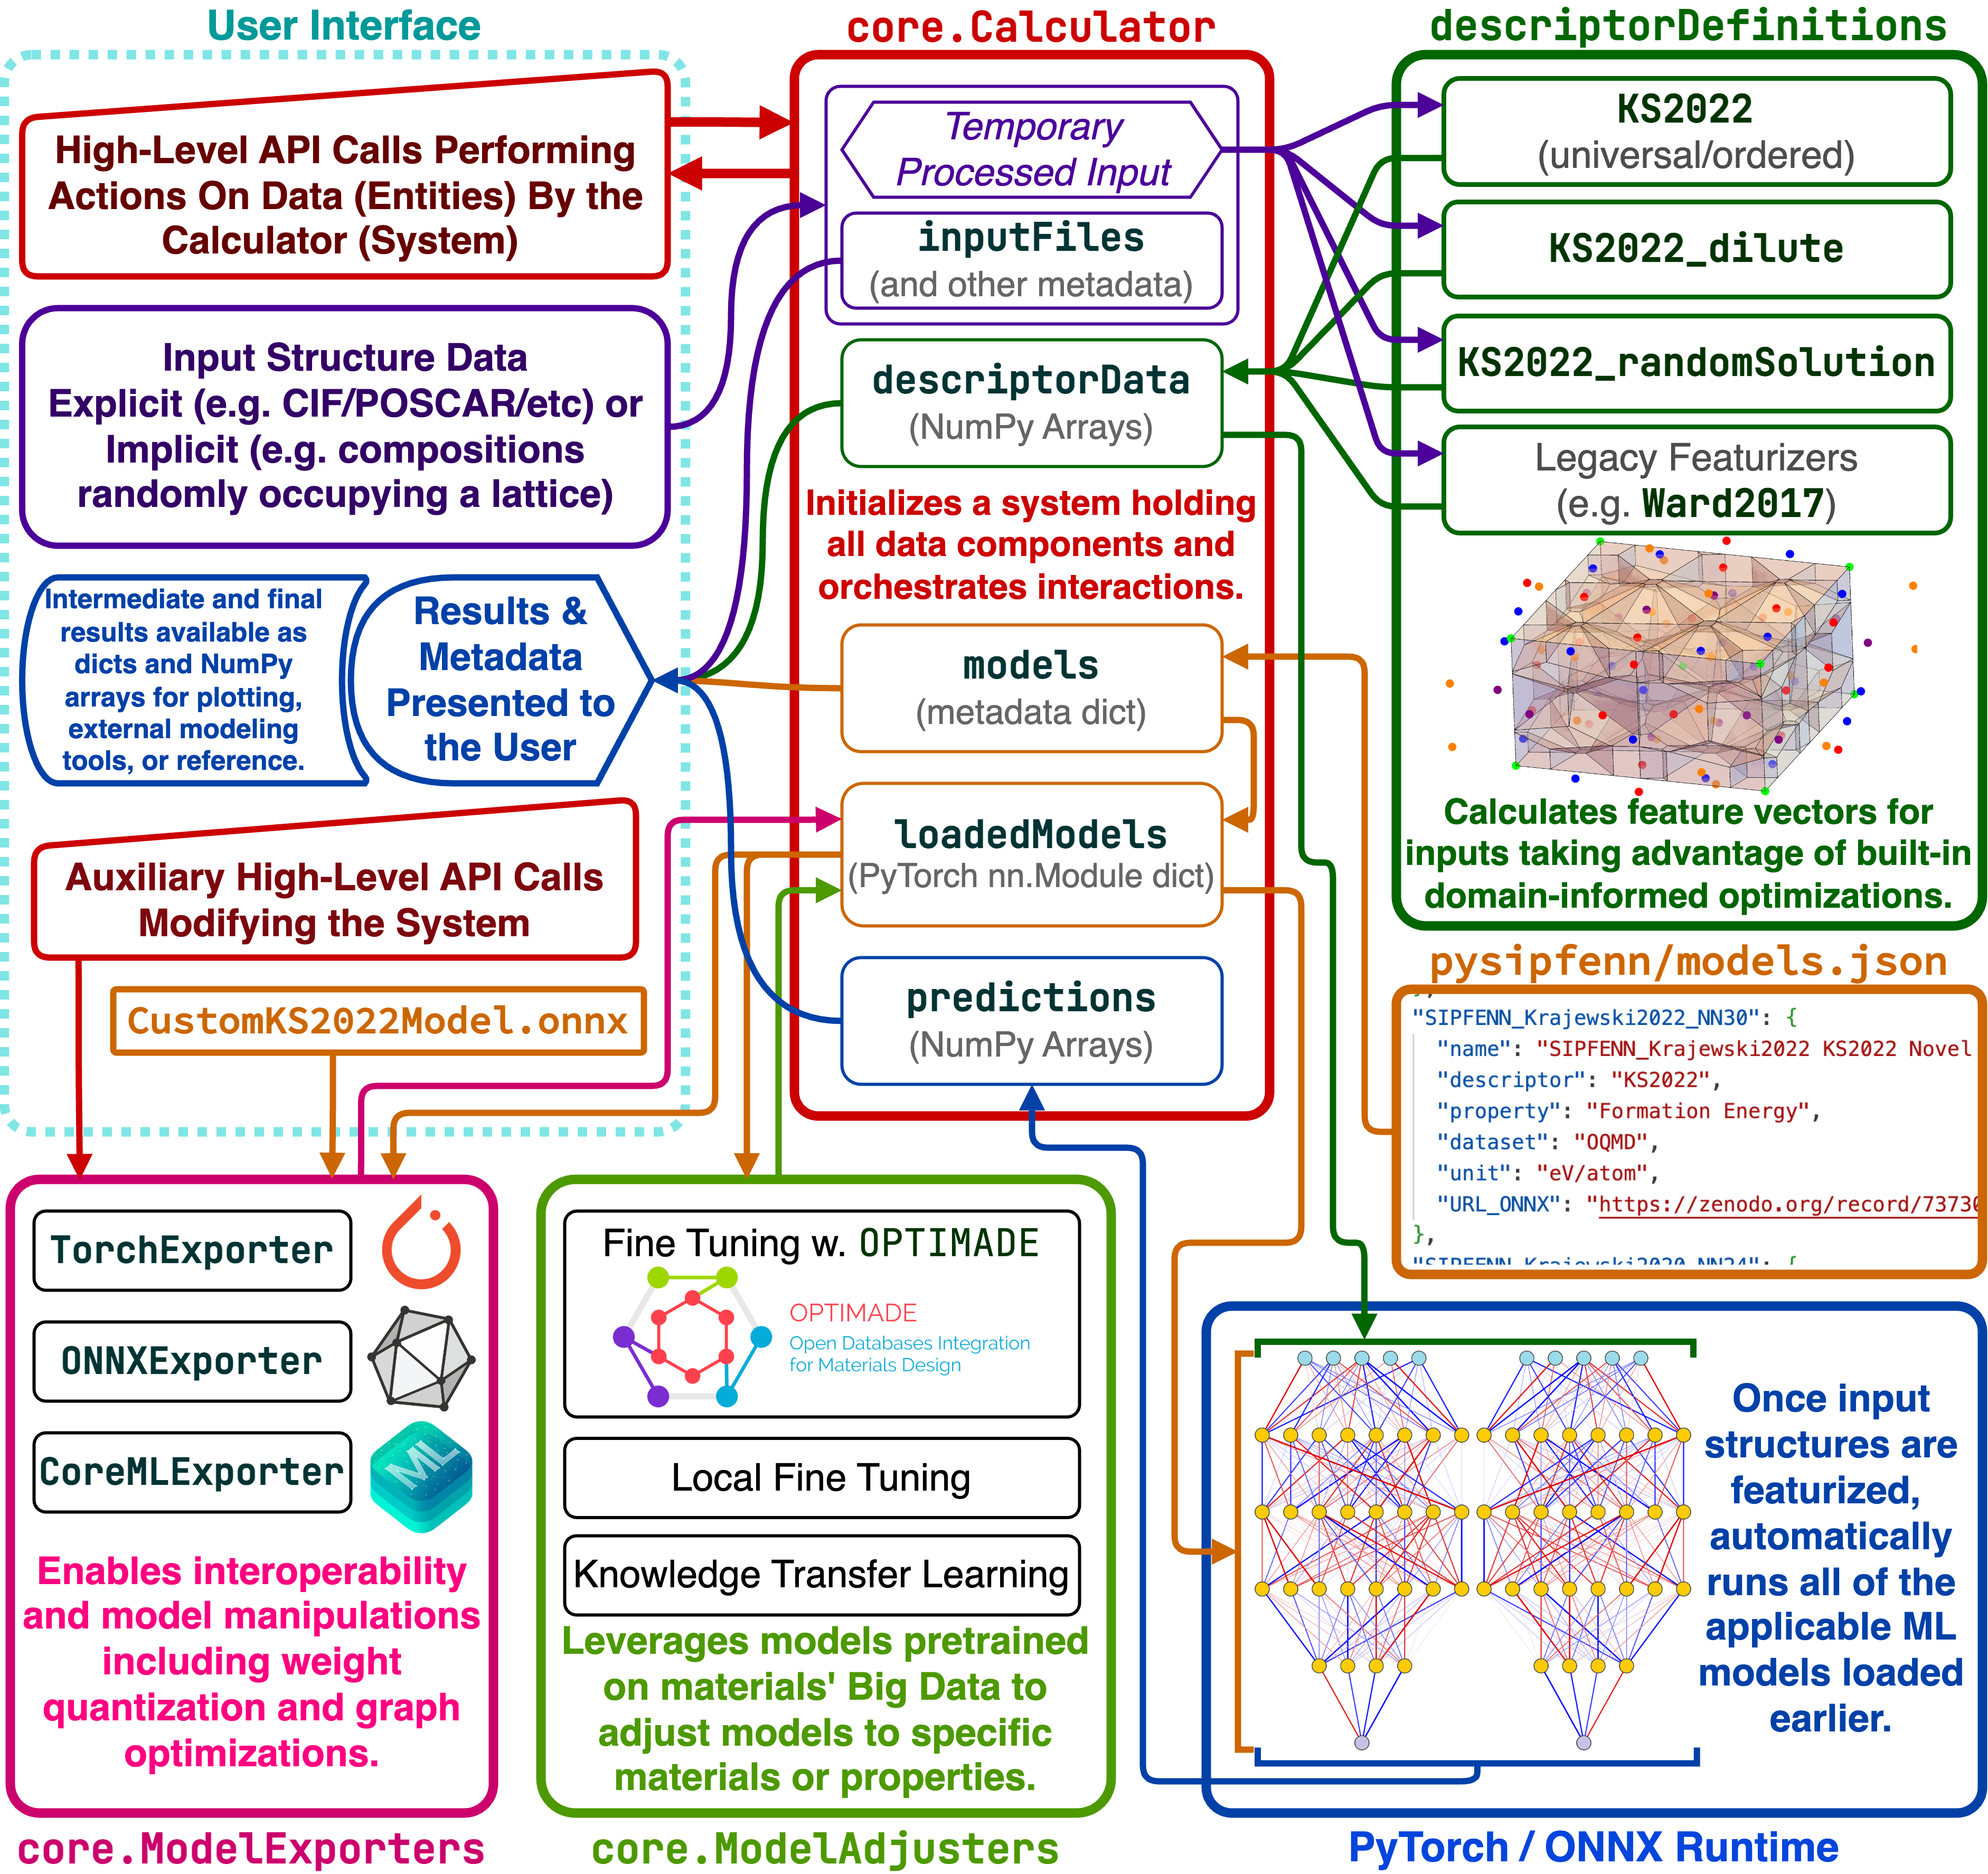
\includegraphics[width=0.85\textwidth]{pysipfenn/pySIPFENN_MainSchematic.png}
    \caption{Main schematic of \texttt{pySIPFENN} framework detailing the interplay of internal components described in Section \ref{pysipfenn:ssec:coreimprovements}. The user interface provides a high-level API to process structural data within \texttt{core.Calculator}, pass it to featurization submodules in \texttt{descriptorDefinitions} to obtain vector representation, then passed to models defined in \texttt{models.json} and (typically) run automatically through all available models. All internal data of \texttt{core.Calculator} is accessible directly, enabling rapid customization. An auxiliary high-level API enables advanced users to operate and retrain the models.}
    \label{pysipfenn:fig:pySIPFENNMainSchematic}
\end{figure}


\subsection{Ward2017 Reimplementation} \label{pysipfenn:ssec:Ward2017Translation}

In their 2017 work \citet{Ward2017} introduced a novel atomic structure featurization concept based on establishing and weighting neighbor interactions by faces from 3D Voronoi tesselation to describe local chemical environments (LCEs) of atomic sites and then performing statistics over them to obtain a global feature vector. The original \texttt{SIPFENN} models \cite{Krajewski2020SIPFENNModels} built on top of this while utilizing an improved, carefully designed deep neural network models to obtain up to 2.5 times lower prediction error on the same dataset \cite{Krajewski2022ExtensibleNetworks}. A detailed description of the descriptor can be found in Section 2.1 of \citet{Krajewski2022ExtensibleNetworks}. In general, the calculation of the \texttt{Ward2017} descriptor consists of three parts:

\begin{itemize}
    \item Calculation of attributes based upon global averages over the components of the structure.
    \item Calculation of attributes based upon local neighborhood averages for each site in the structure.
    \item Calculation of more complex attributes based upon averages over paths in the structure.
\end{itemize}

\citet{Ward2017} implemented the above calculations in Java, which was popular at the time; while most of the current machine-learning packages use almost exclusively Python (e.g., \texttt{scikit-learn} \cite{PedregosaFABIANPEDREGOSA2011Scikit-learn:Python} and \texttt{PyTorch} \cite{Paszke2019PyTorch:Library}), making it cumbersome to use Java. Even more critically, the original Java implementation was not computationally efficient (as explored in Sections \ref{pysipfenn:sec:ordered}, \ref{pysipfenn:sec:dilute}, and \ref{pysipfenn:sec:randomsolutions}), and enabling tools were not supported in Java.

In the present work, authors have reimplemented \citet{Ward2017} from scratch in Python as a standalone submodule for \texttt{pySIPFENN}, which calculates all 271 features within numerical precision, except for three performing a random walk on the structure, which is stochastic in nature and results in slightly different final values due to a different seed. The Voronoi tessellation has been implemented with \texttt{Voro++} \cite{Rycroft2007MultiscaleFlow, Rycroft2009Voro++:C++, Lu2023AnCells} and all numerical operations were written using \texttt{NumPy} \cite{Harris2020ArrayNumPy} arrays to greatly speed up the calculations and make the efficient utilization of different computing resources, such as GPUs, easy to implement.

\subsection{KS2022 Feature Optimization} \label{pysipfenn:ssec:ks2022features}

Typically, during feature engineering, researchers first attempt to collect all features expected to enable good inference and then remove some based on the interplay of several factors:
\begin{enumerate}
    \item \textbf{Low impact} on the performance, which increases the representation memory requirements and possibly increases the risk of overfitting to both systematic and random trends. 
    \label{pysipfenn:item:featureoptimize1}
    \item \textbf{High computational cost}, which limits the throughput of the method deployment.
    \label{pysipfenn:item:featureoptimize2}
    \item \textbf{Unphysical features or feature representations} which can improve model performance against well-behaving benchmarks covering a small subset of the problem domain but compromise model interpretability and extrapolation ability in unpredictable ways.
    \label{pysipfenn:item:featureoptimize3}
\end{enumerate}

The \texttt{KS2022} feature set, added in \texttt{pySIPFENN v0.10} in November 2022, is a significant modification of the \texttt{Ward2017} \cite{Ward2017}, which focuses on points \ref{pysipfenn:item:featureoptimize2} and \ref{pysipfenn:item:featureoptimize3} above, while enabling optimizations described in Sections \ref{pysipfenn:sec:ordered} through \ref{pysipfenn:sec:randomsolutions} and delegating the removal of low-impact features to modeling efforts and keeping featurization as problem-independent as possible.

First, all 11 features relying on representation of crystal symmetry space groups with space group number \texttt{float}s rather than classes (e.g. using one-hot vectors) have been removed due to the unphysical nature of such representation leading to, for instance, BCC ($229$) being much closer to FCC ($225$) than to just slightly uniaxially distorted BCC ($139$), which itself would be very close to trigonal structures. 

Next, featurization code has been thoroughly profiled in regard to time spent on the execution of feature-specific subroutines and analyzed in the context of feature importance identified in the past work \cite{Krajewski2022ExtensibleNetworks}. This led to the removal of the 1 \textit{CanFormIonic} feature, which relied on combinatorically expensive guessing of oxidation states, and 3 features based on Warren-Cowley (WC) parameters \cite{Cowley1950AnAlloys}, which were relatively very expensive without significantly contributing to the performance due to scarcity of disordered structures in most atomistic datasets. However, the authors intend to add them back in future problem-specific feature sets using a recently released high-performance library by \citet{Gehringer2023ModelsSimple}. 

Together, 15 features were removed, bringing the total number of the \texttt{KS2022} features to $256$ while disproportionately improving the featurization speed. For instance, in the case of featurization of 30 sites in a disordered (no symmetry) structure, \texttt{KS2022} is $2.3$ times faster than \texttt{Ward2017} ($430$ms vs $990$ms single-threaded on Apple M2 Max).

\section{Optimizations for Ordered Structures} \label{pysipfenn:sec:ordered}

Modeling of disordered materials is a critical area of research \cite{Zaki2023Glassomics:Intelligence}; however, the vast majority of atomistic ab initio datasets used for ML studies focuses on highly symmetric ordered structures because of their high availability and ability to model complex phenomena in a holistic fashion if local ergodicity can be established \cite{Liu2022TheoryTheorem, Liu2023ThermodynamicsPerspectives}. One evidence of the focus on such data is the fact that out of $4.4$ million atomic structures in \texttt{MPDD} \cite{Krajewski2021MPDD:Database}, which includes both DFT-based \cite{Saal2013MaterialsOQMD, Kirklin2015TheEnergies, Shen2022ReflectionsOQMD, Curtarolo2013AFLOW:Discovery, Toher2018TheDiscovery, Jain2013Commentary:Innovation, Choudhary2020TheDesign, Merchant2023ScalingDiscovery} and experimental \cite{Grazulis2009CrystallographyStructures, Grazulis2012CrystallographyCollaboration, Grazulis2019CrystallographyPerspectives} data, only $54$ thousand or $1.25\%$ lack any symmetry. It is also worth noting that this number used to be much lower before the recent publication of the \texttt{GNoME} dataset by Google DeepMind \cite{Merchant2023ScalingDiscovery}, which accounts for around $\frac{3}{4}$ of them. 

In the case of remaining $98.75\%$ structures, a 3-dimensional crystallographic spacegroup is defined for each of them along with corresponding \emph{Wyckoff positions} (designated by letters) which are populated with either zero (empty), one (when symmetry-fixed), or up to infinitely many (typically up to a few) atoms forming a set of symmetry-equivalent sites called \emph{crystallographic orbits} \cite{Muller2006RemarksPositions}. When these crystallographic orbits are collapsed into atoms occupying a unit cell, each is repeated 
based on the \emph{multiplicity} associated with the Wyckoff position it occupies, which can range from 1 up to 192 (e.g., position l in Fm-3m/225), with values 1, 2, 3, 4, 6, 8, 16, 24, 32, 48, and 96 being typical \cite{Mehl2016ThePrototypes} even in compositionally simple materials like one of the experimentally observed allotropes of pure silicon with atoms at the 8a, 32e, and 96g positions \cite{Gryko2000Low-densityGap}. For certain crystal lattice types, the multiplicity can be somewhat reduced by redefining their spatial periodicity with so-called \textit{primitive} unit cells, like in the case of the aforementioned Si allotrope, in which primitive unit cell has 4 times fewer (34) sites but still over 10 times more than the 3 unique crystallographic orbits.

This presents an immediate and previously untapped opportunity for multiplying the computational performance of most atomistic featurizers (e.g., \texttt{Matminer} \cite{Ward2018Matminer:Mining}) and ML models \cite{Ward2017, Chen2019GraphCrystals, Jha2019IRNet, Krajewski2022ExtensibleNetworks, Choudhary2021AtomisticPredictions, Deng2023CHGNetModelling, Davariashtiyani2023FormationRepresentation, Schmidt2023Machine-Learning-AssistedMaterials, Banik2024EvaluatingMaterials, Hu2021Atomtransmachine:Learning}, which nearly always process all atoms given in the input structure occasionally converting to primitive unit cell in certain routines (\texttt{CHGNet} \cite{Deng2023CHGNetModelling}), unless they operate on different occupancies of the same structure \cite{Crivello2022SupervisedExample}. This allows for a proportional decrease in both CPU/GPU time and memory footprint. The general-purpose \texttt{KS2022} in \texttt{pySIPFENN} uses high-performance symmetry analysis library \texttt{spglib} \cite{Togo2018Spglib:Search} to automatically take advantage of this whenever possible, as depicted in the schematic in Figure \ref{pysipfenn:fig:ks2022}. It shows an interesting example of a topologically close-packed $\sigma$ phase, which is critical to model in a wide range of metallic alloys \cite{Joubert2008CrystalPhase} but challenging in terms of combinatorics because of 5 unique sites that can be occupied by many elements \cite{Choi2019ADesign, Ostrowska2020ThermodynamicW} making it a very active area of ML modeling efforts \cite{Crivello2022SupervisedExample, Zha2024ApplyingEnergy} in the thermodynamics community.

\begin{figure}[h]
    \centering
    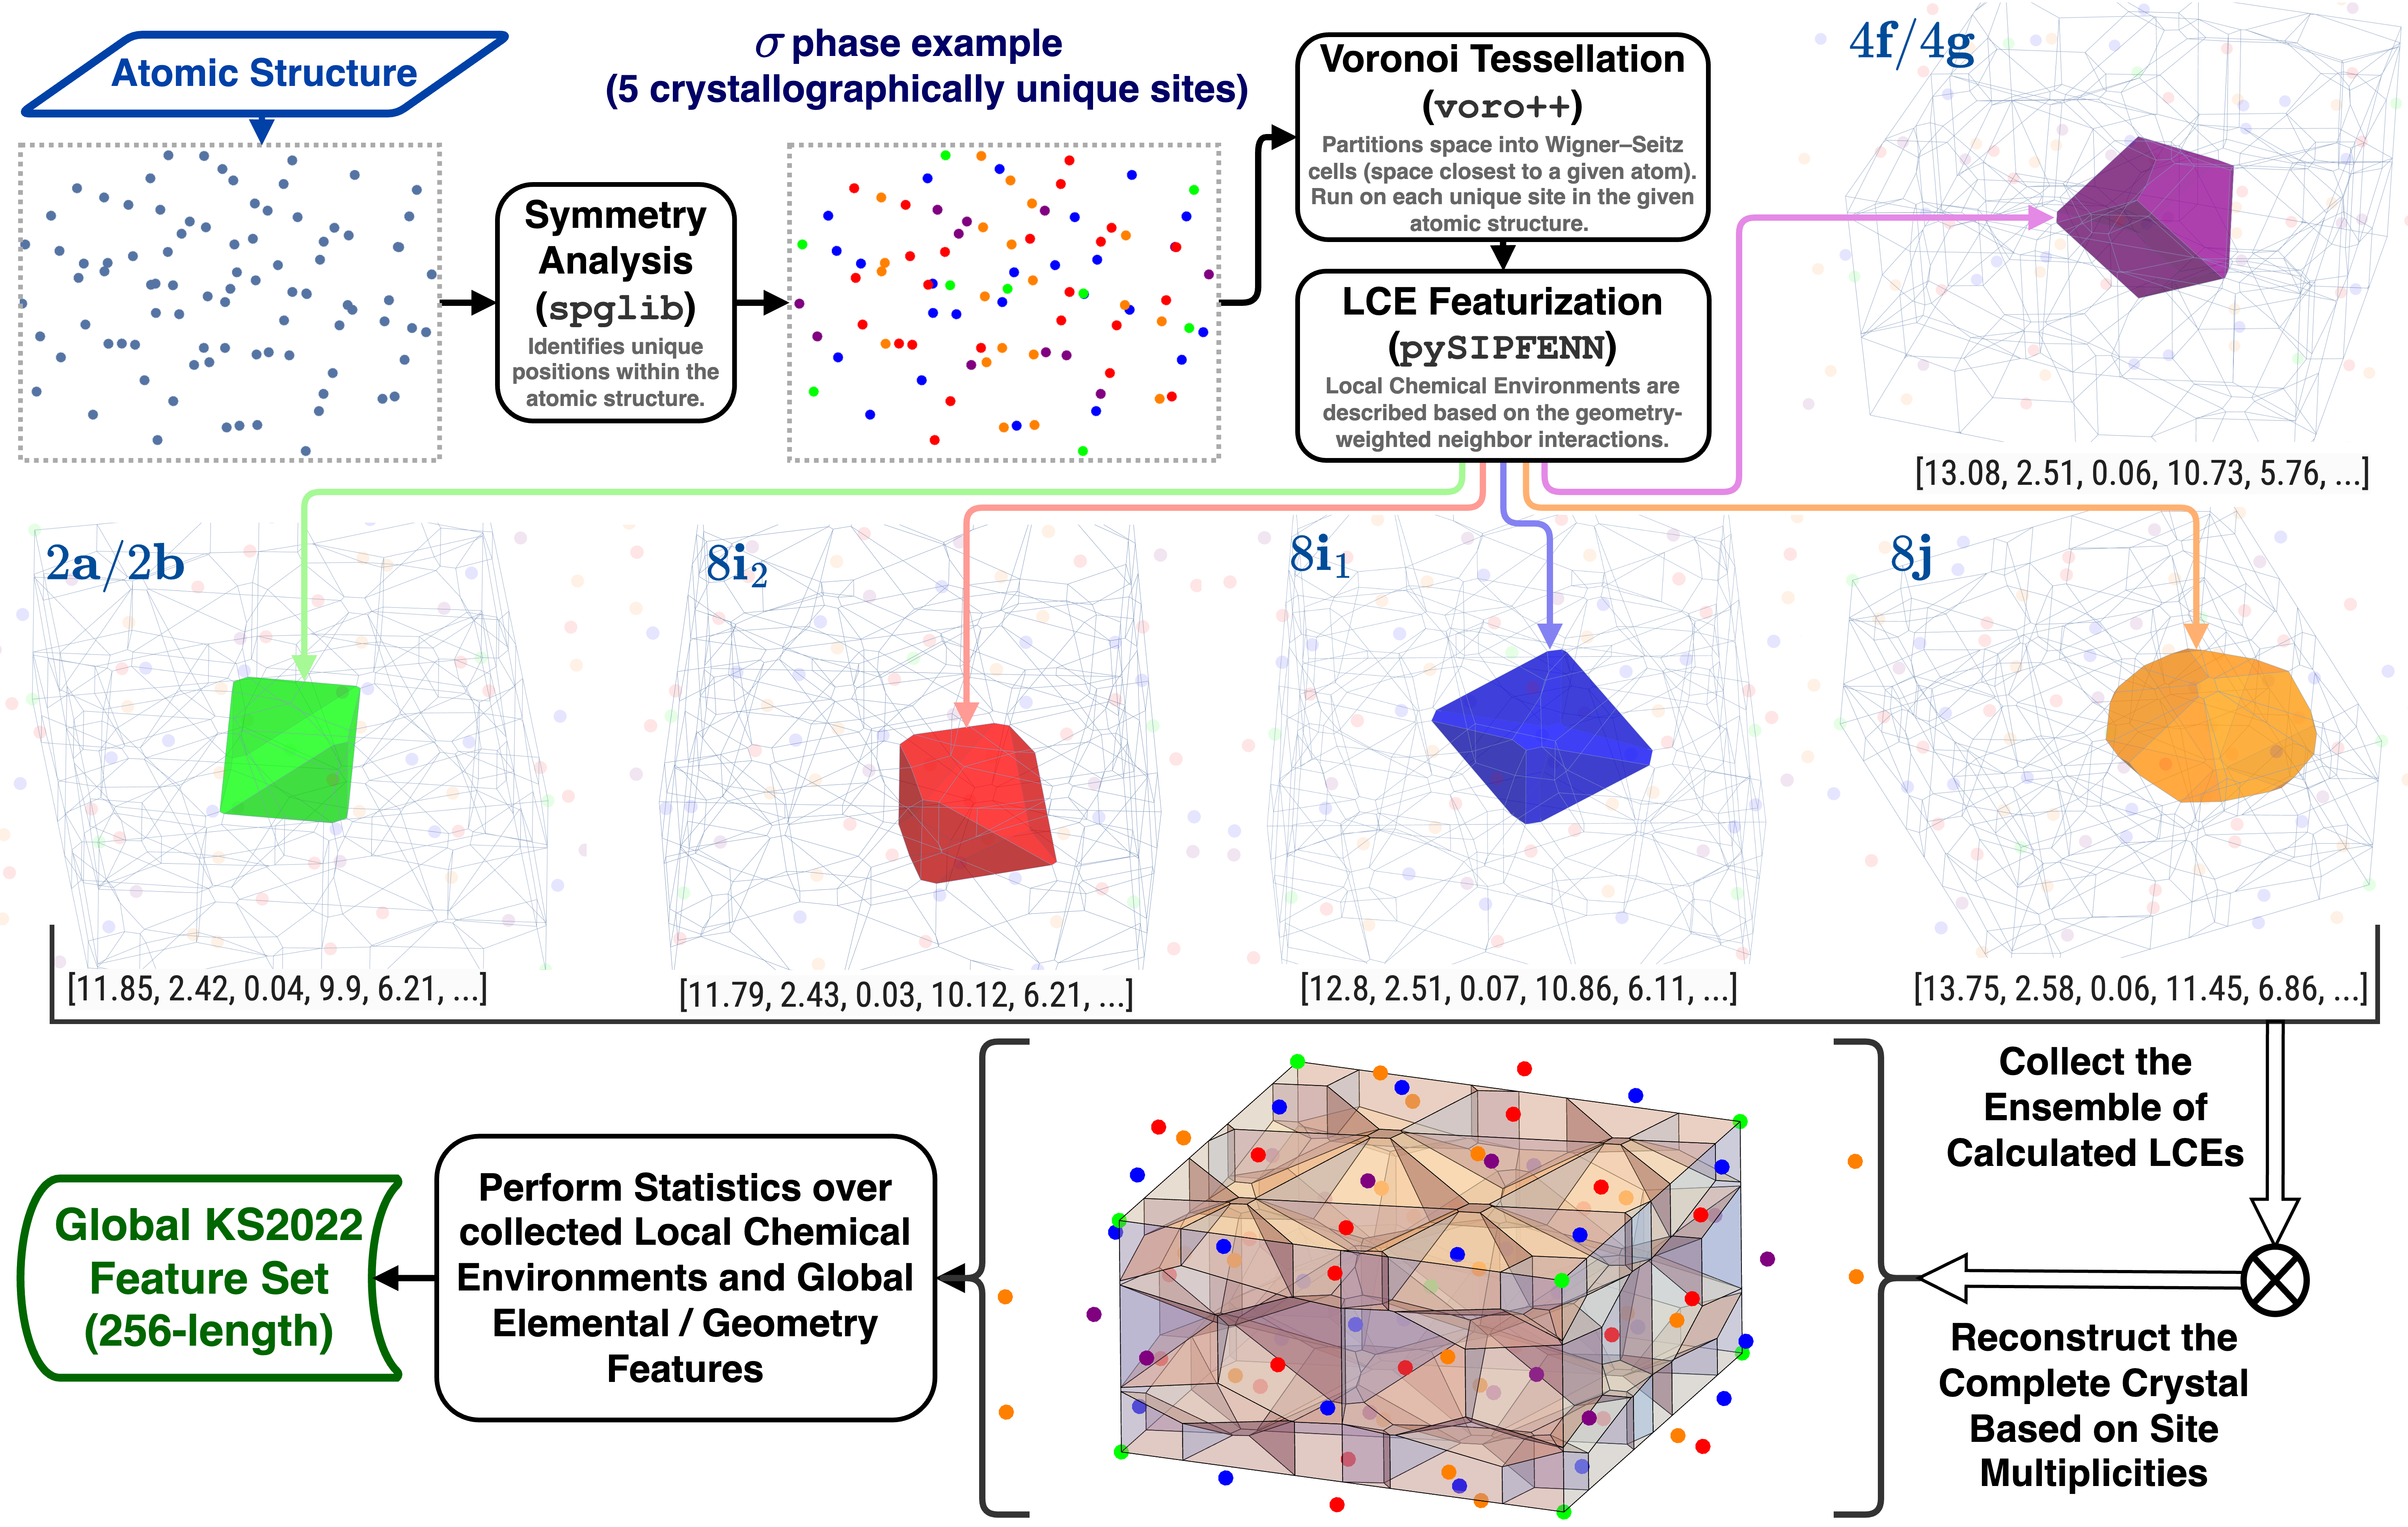
\includegraphics[width=0.98\textwidth]{pysipfenn/KS2022.png}
    \caption{
    Schematic of the general-purpose \texttt{KS2022} featurization routine with built-in optimization for ordered structures. First, the atomic structure (in \texttt{pymatgen Structure} object format \cite{Ong2013PythonAnalysis}) is loaded, and sites in it are annotated with their crystallographic orbits using \texttt{spglib} \cite{Togo2018Spglib:Search}. Then, one site is selected from each orbit to form a set of unique sites, for which Wigner-Seitz cells (depicted as colored polyhedra) are calculated with \texttt{Voro++} \cite{Rycroft2007MultiscaleFlow, Rycroft2009Voro++:C++, Lu2023AnCells} and featurized to get site-specific local chemical environment (LCE) descriptors. The complete site ensemble is then reconstructed based on multiplicities of Wyckoff positions corresponding to the sites. A non-trivial example of $\sigma$-phase with 30 atoms belonging to 5 crystallographic orbits with interesting Wigner-Seitz cells (relative to usually shown FCC/BCC ones \cite{Bohm1996VoronoiLattices}) has been depicted.
    }
    \label{pysipfenn:fig:ks2022}
\end{figure}

In the case of \texttt{KS2022} featurizer, running the same 30-atom test as in Section \ref{pysipfenn:ssec:ks2022features} but on $\sigma$ phase takes on average $84$ms or is 5.1 times faster thanks to processing 6 times less sites. Similar results should be (a) quickly achievable with any other featurizer processing individual sites, including most graph representations embedding local environments (e.g., \texttt{MEGNet} \cite{Chen2019GraphCrystals}) or deconstructing graphs into graphlets (e.g., \texttt{minervachem} molecule featurizer \cite{Tynes2024LinearCheminformatics}), and (b) possible with convolution-based models operating on graphs (e.g., \texttt{ALIGNN} \cite{Choudhary2021AtomisticPredictions}) or voxels \cite{Davariashtiyani2023FormationRepresentation} through custom adjustments to the specific convolution implementation. In the case of voxel representations and any other memory-intense ones, it may also be beneficial to utilize this approach to compress them when transferring between devices like CPU and GPU or across an HPC network.


\section{Optimizations for Dilute, Defect, and Doped Structures} \label{pysipfenn:sec:dilute}

The optimization strategy in Section \ref{pysipfenn:sec:ordered} ensures that only the sites that are \emph{guaranteed} to be \emph{crystallographically unique} are processed through featurization or graph convolution and is directly applicable to the vast majority of both data points and literature methods. However, in the case of methods relying on describing the immediate neighbors, whether through Wigner-Seitz cell (see Fig. \ref{pysipfenn:fig:ks2022}) or subgraph (see, e.g., \cite{Chen2019GraphCrystals}), one can achieve further efficiency improvements by considering which sites are \emph{guaranteed} to be \emph{unique under the representation}.

There are several classes of atomic structures where the distinction above makes a difference, but the room to improve is exceptionally high when one site in an otherwise highly symmetric structure is modified, leading to a structure that, depending on the context, will be typically called \emph{dilute} when discussing alloys \cite{Chong2021CorrelationAlloys}, \emph{doped} when discussing electronic materials \cite{Chen2022InteractionStudy}, or said to have \emph{defect} in a more general sense \cite{Castleton2009DensitySupercells}. Throughout \texttt{pySIPFENN}'s codebase and the rest of this work, the single term \emph{dilute} is used to refer to all of such structures due to authors' research focus on Ni-based superalloys at the time when optimizations below were made public in February 2023.

To visualize the concept, one can consider, for instance, a 3x3x3 body-centered cubic (BCC) conventional supercell (54 sites) and call it \textit{base structure}. If it only contains a single specie, then \texttt{KS2022} from Section \ref{pysipfenn:sec:ordered} will recognize that there is only one crystallographic orbit and only process that one. However, if a substitution is made at any of the 54 equivalent sites, the space group will change from Im-3m (229) to Pm-3m (221), with 8 crystallographic orbits on 7 Wyckoff positions; thus, the default \texttt{KS2022} featurizer will process 8 sites. 
At the same time, several of these crystallographic orbits will be differentiated \emph{only} by the orientation and distance to the dilute (substitution) site, which \emph{does} affect ab initio calculation results (e.g., vacancy formation energy vs supercell size \cite{Hargather2022ANi}), but is \emph{guaranteed} to \emph{have no effect on the model's representation} because of the exact same neighborhood configuration (including angles and bond lengths) if conditions given earlier are met. Thus, it only requires adjustments to the site multiplicities or convolution implementation (simplified through, e.g., a Markov chain). In the particular dilute-BCC example at hand, depicted in Figure \ref{pysipfenn:fig:KS2022dilute}, there are 4 such \emph{representation-unique} crystallographic orbits, i.e., 1 with the dilute atom, 2 neighboring the dilute atom sharing either large hexagonal (1st nearest neighbor shell) or small square face (2nd nearest neighbor shell), and 1 non affected by the dilute atom which is equivalent to the remaining 4 orbits; thus reducing number of sites that need to be considered by a factor of 2.

The \texttt{KS2022\_dilute} featurization routine, schematically depicted in Figure \ref{pysipfenn:fig:KS2022dilute}, conveniently automates the above process for both simple cases like aforementioned substitution in pure element and complex cases like introducing a dilute atom at the 2a/2b orbit in $\sigma$-phase (green cell in Fig. \ref{pysipfenn:fig:ks2022}), by performing independent identification of crystallographic orbits in the dilute structure and base structure, followed by identification of the dilute site and its configuration to establish orbit equivalency under \texttt{pySIPFENN}'s \texttt{KS2022} representation, to finally reconstruct complete site ensemble of the dilute structure.

\begin{figure}[h]
    \centering
    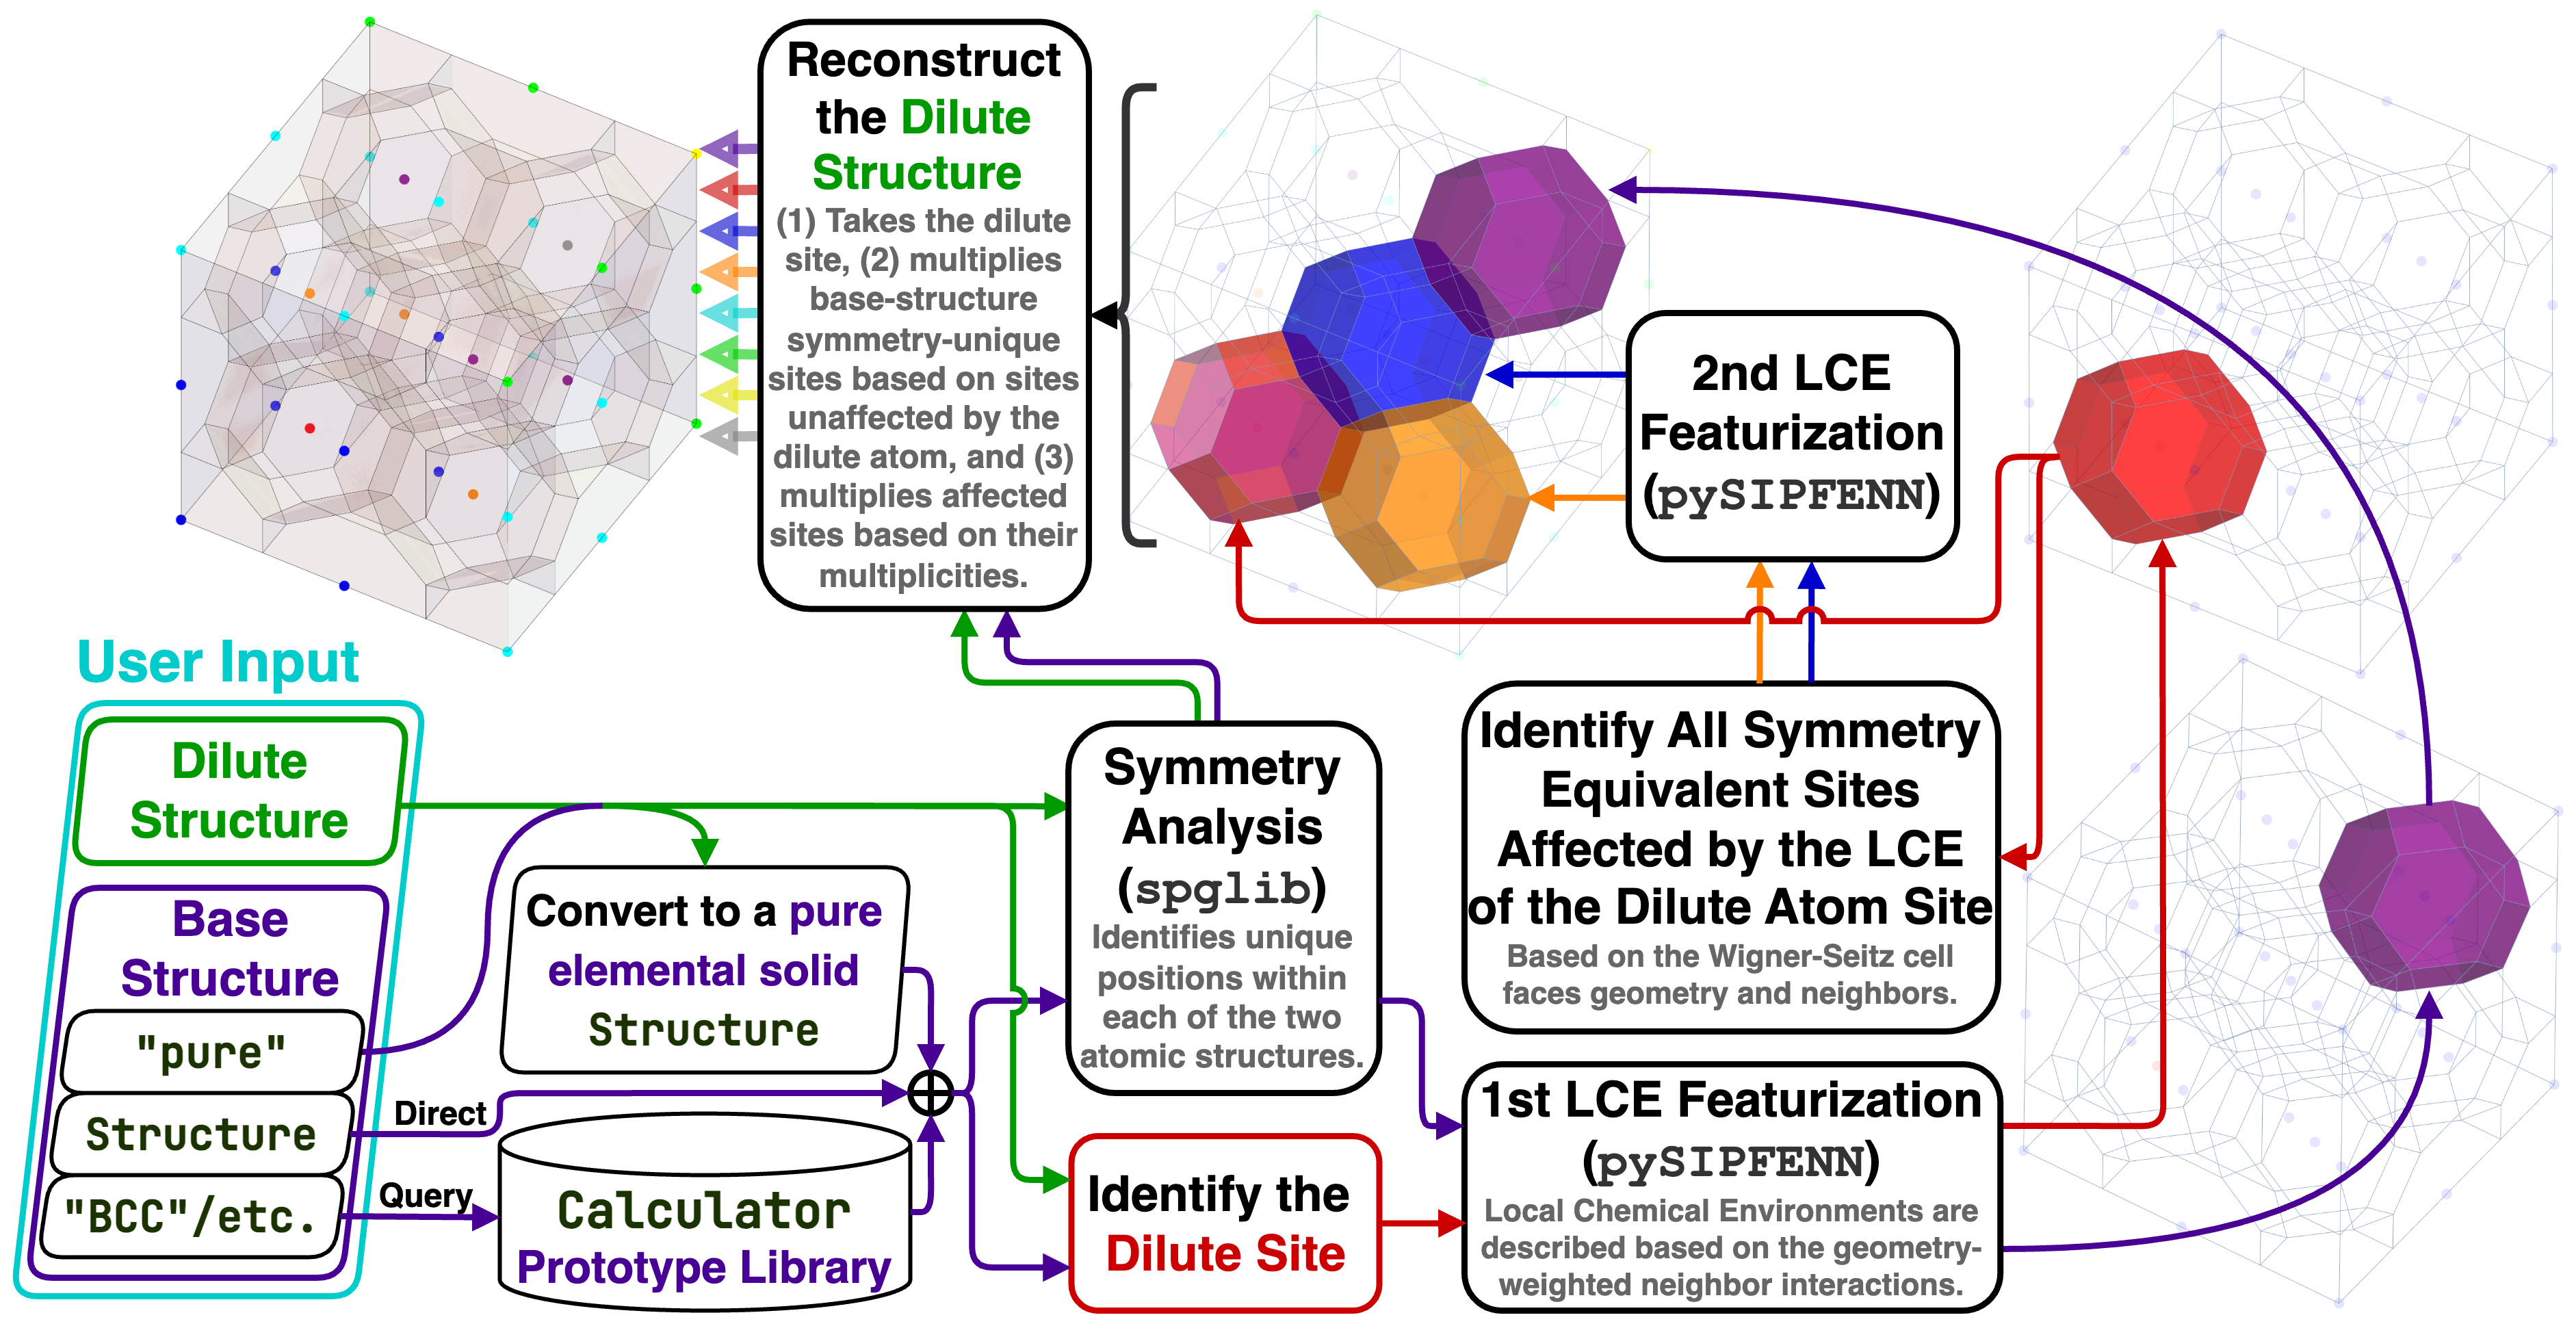
\includegraphics[width=0.85\textwidth]{pysipfenn/KS2022_dilute.png}
    \caption{Core schematic of the \texttt{KS2022\_dilute} featurizer. The dilute structure is compared to either the explicit or implicit base structure to identify the dilute site, which is then featurized alongside all crystallographically unique sites in the base structure. Information extracted from dilute structure featurization is then used to identify previously-equivalent sites affected by it, which go through the second round of featurization. Lastly, the complete ensemble is reconstructed, and \texttt{KS2022} are obtained. BCC supercell is used as an example.}
    \label{pysipfenn:fig:KS2022dilute}
\end{figure}

In the case of \texttt{KS2022\_dilute} implementation run on the dilute BCC supercell shown in Figure \ref{pysipfenn:fig:KS2022dilute}, the efficiency is improved nearly proportionally to the reduction in the number of considered sites, averaging $51$ms vs $98$ms \texttt{KS2022}, signifying 1.9 computational cost reduction relative to calculating all crystallographically unique sites. Or around 10-fold computational cost reduction relative to the standard \cite{Ward2017, Chen2019GraphCrystals, Jha2019IRNet, Krajewski2022ExtensibleNetworks, Choudhary2021AtomisticPredictions, Deng2023CHGNetModelling, Davariashtiyani2023FormationRepresentation, Schmidt2023Machine-Learning-AssistedMaterials} approach of processing all sites ($494$ms), while producing precisely the same results (within the numerical precision).


\section{Optimizations for Random Solid Solutions} \label{pysipfenn:sec:randomsolutions}

Sections \ref{pysipfenn:sec:ordered} and \ref{pysipfenn:sec:dilute} have demonstrated how recognition of symmetry in ordered structures can guarantee equivalency of sites and how understanding the character of featurization can further extend that notion of equivalency so that the ML representations of all sites can be obtained efficiently up to an order of magnitude faster. Random solid solutions are the conceptually opposite class of atomic structures, where the \emph{lack of} symmetry or site equivalency is \emph{guaranteed}, yet featurizing them requires one to solve the same problem of efficiently obtaining the ML representations of all sites present, which also happen to be infinite.

Typically, in the ab initio community, random solid solutions are represented using Special Quasirandom Structures (SQS) introduced in landmark 1990 work by \citet{Zunger1990SpecialStructures}, which are \emph{the} best structures to match neighborhood correlations in a purely random state given component ratios and number of atoms to use, hence the name \emph{special}. For many years, finding SQS structures required exponentially complex enumeration of all choices and was limited to simple cases until another critical work by \citet{VanDeWalle2013EfficientStructures}, which used simulated annealing Monte Carlo implemented through \texttt{ATAT} software to find these special cases much faster, exemplified through the relatively complex $\sigma$-phase and enabling the creation of SQS libraries used in thermodynamic modeling \cite{vandeWalle2017SoftwareData}.

However, the direct use of an SQS may not be the optimal choice for structure-informed random solid solution featurization due to several reasons. Firstly, as discussed by \citet{VanDeWalle2013EfficientStructures}, SQS can be expected to perform well on purely fundamental grounds for certain properties like total energy calculations, but one has to treat them with caution because different properties will depend differently on the correlation and selecting the SQS may be suboptimal. Building up on that, one could, for instance, imagine a property that depends strongly on the existence of low-frequency, high-correlation regions catalyzing a surface reaction or enabling nucleation of a dislocation. In terms of ML modeling, this notion is taken to the extreme with calculated features being both very diverse and numerous while being expected to be universal surrogates for such mechanistically complex properties.

Secondly, SQSs that can be generated in a reasonable time are limited in terms of the number of atoms considered, causing quantization of the composition. This is not an issue if a common grid of results is needed, e.g., to fit CALPHAD model parameters \cite{vandeWalle2017SoftwareData} or to train a single-purpose ML model \cite{Tandoc2023MiningAlloys}, but it becomes a critical issue if one needs to accept an arbitrary composition as the ML model and SQS would have to be obtained every time. This issue is further amplified by the rapidly growing field of compositionally complex materials (CCMs), which exist in vast many-component compositional spaces prohibiting SQS reuse even at coarse quantizations \cite{Krajewski2024Nimplex} while being a popular deployment target for both forward and inverse artificial intelligence methods \cite{Catal2023MachineProperties, Rao2022MachineDiscovery, Debnath2023ComparingAlloys} due to their inherent complexity.

Based on the above, it becomes clear that costly computing of an SQS structure would have to be done for every ML model, and it would not be consistent between chemistries and complexities. At the same time, the primary motivation for limiting the number of sites for ab initio calculations is gone since \texttt{KS2022} can featurize over 1,000 sites per second on a laptop (Apple M2 Max run in parallel). 

Thus, the objective of optimization is shifted towards consistency in convergence to feature vector values at infinity. To accomplish that, \texttt{pySIPFENN} goes back to random sampling but at a large scale and \emph{individually monitoring the convergence of every feature} during the expansion procedure, implemented through \texttt{KS2022\_randomSolutions} and depicted in Figure \ref{pysipfenn:fig:KS2022randomSolution}, to ensure individual convergence. 


\begin{figure}[h]
    \centering
    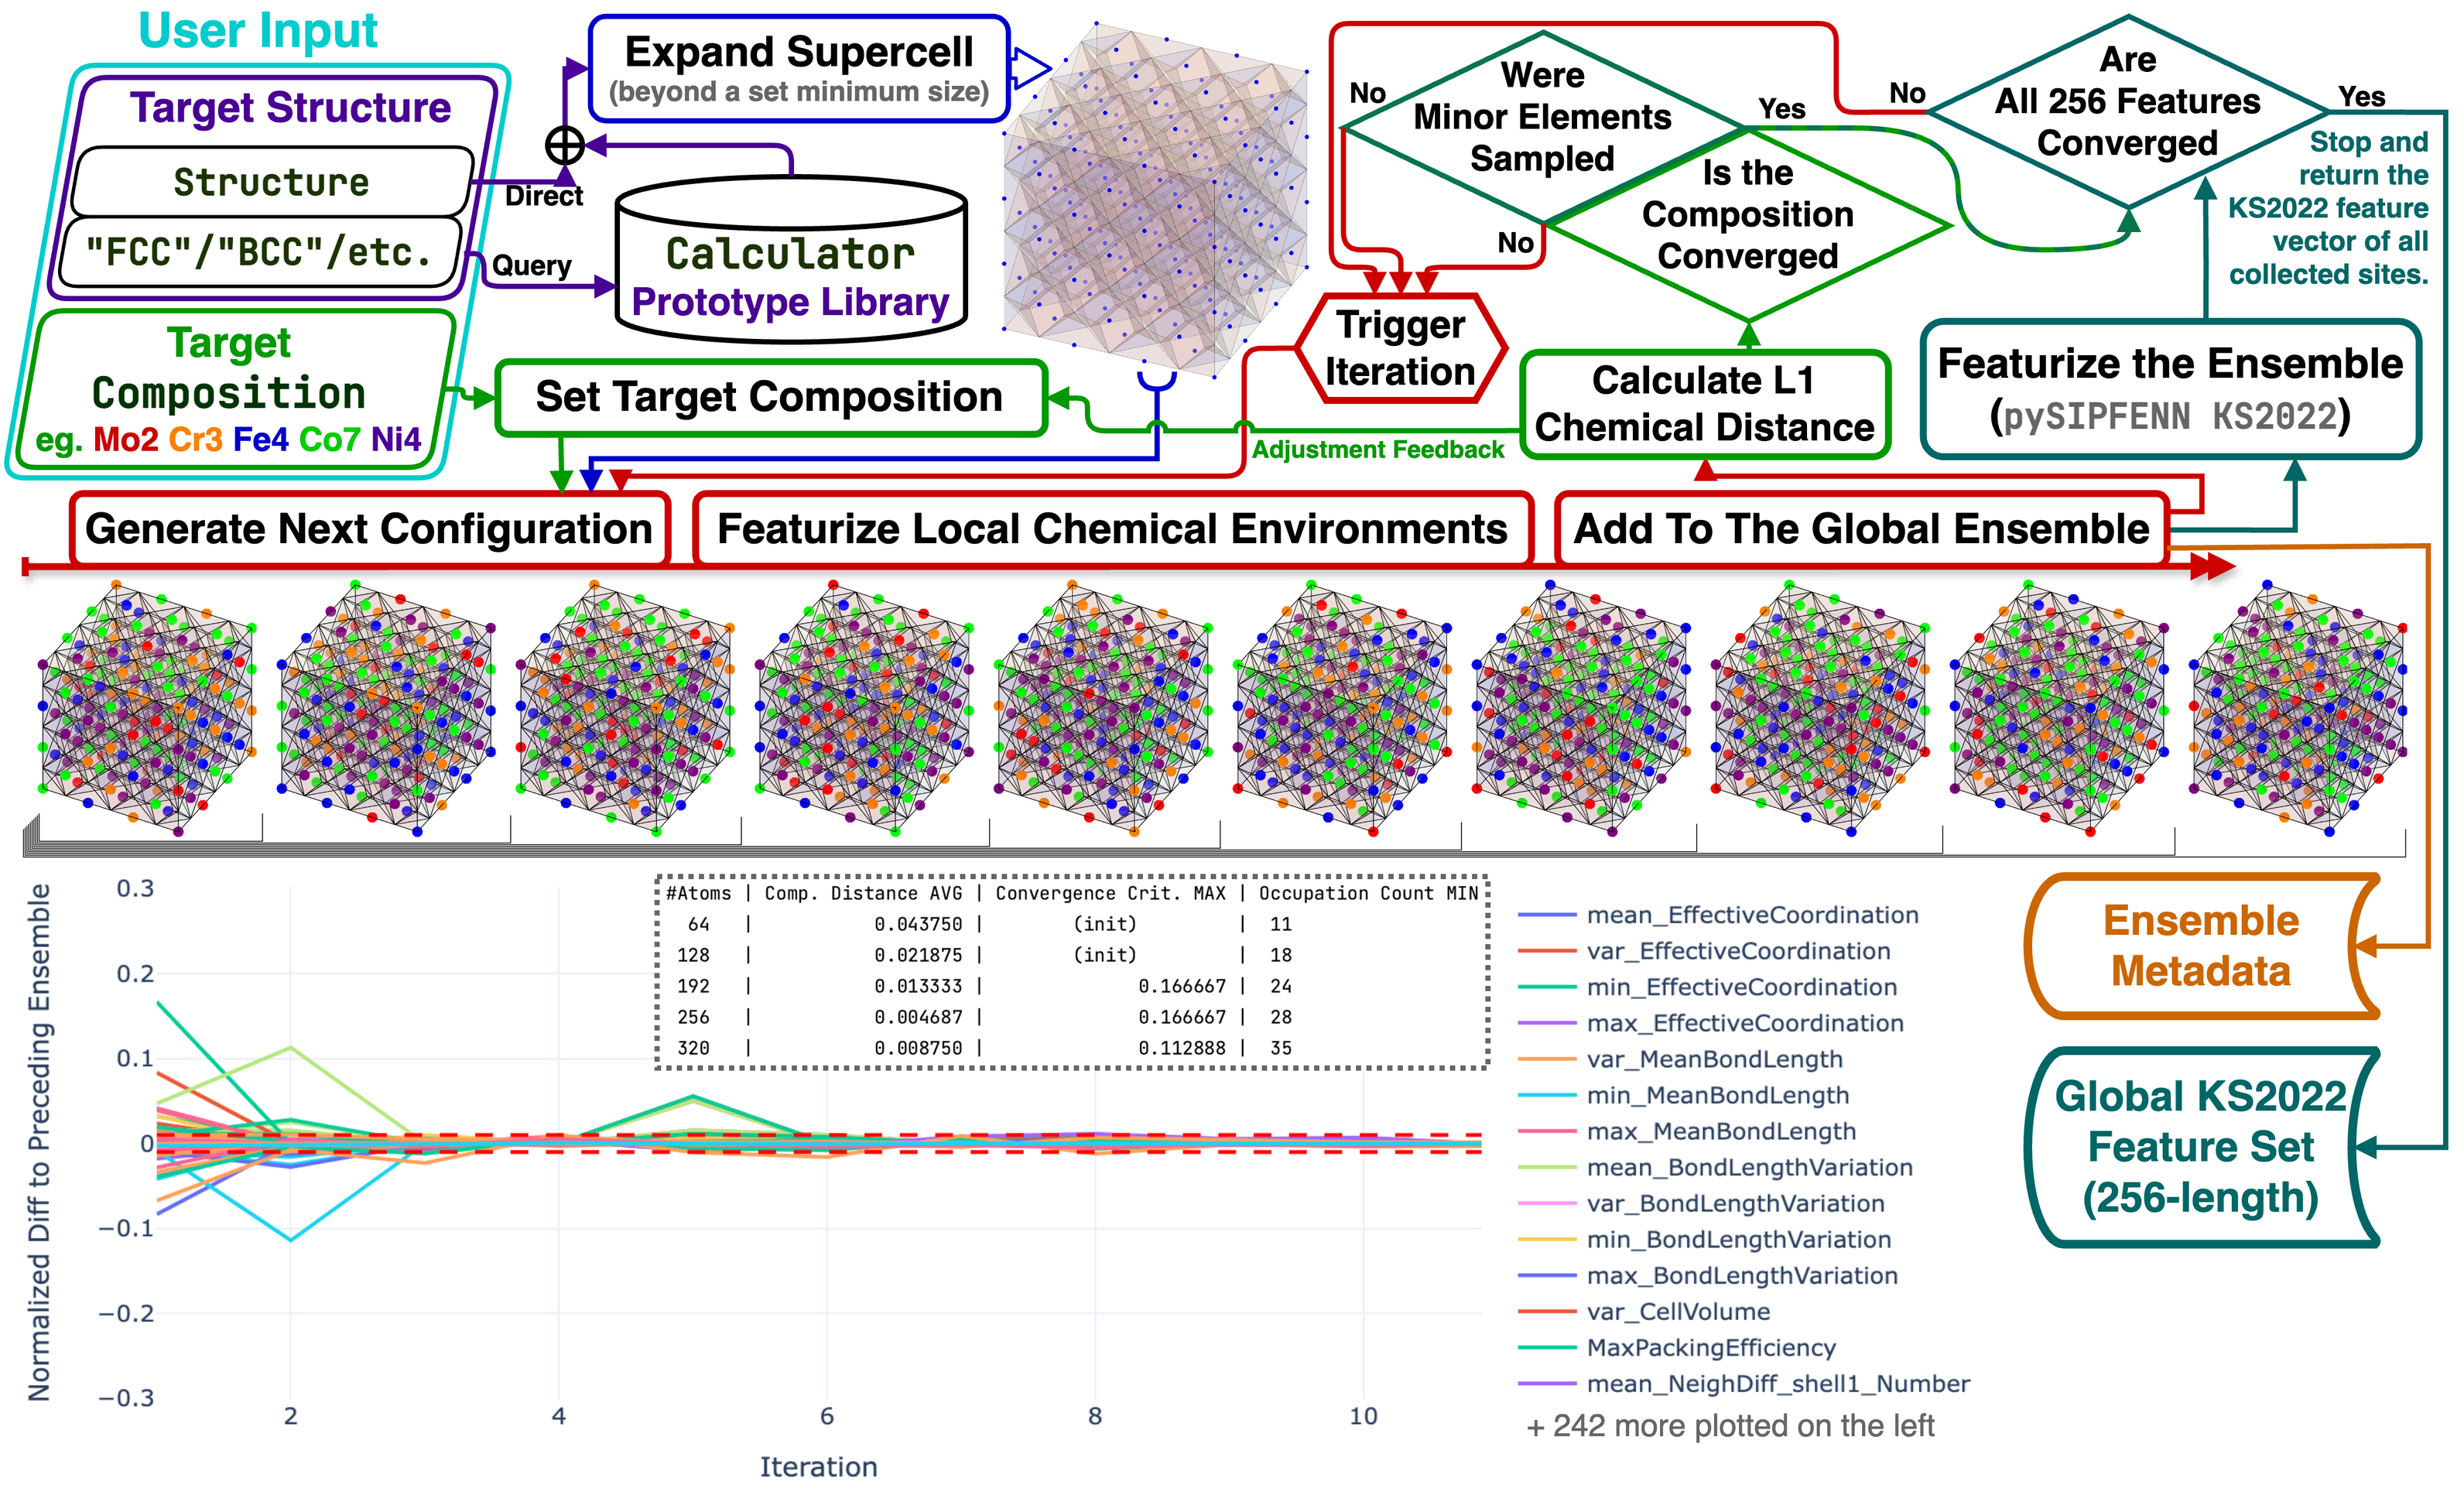
\includegraphics[width=0.95\textwidth]{pysipfenn/KS2022_randomSolution.png}
    \caption{
    Core schematic of the \texttt{KS2022\_randomSolutions} featurizer. The target structure given explicitly or implicitly is expanded to form a (lattice) (i.e. template) supercell. It is then iteratively populated with target composition (slightly adjusted each time) and divided into individual sites, which are featurized (like in \texttt{KS2022}) and added to the global ensemble. The process repeats until the composition is converged, all species have had a chance to occur, and \emph{every individual feature} has converged. Lastly, the global \texttt{KS2022} feature vector and metadata are returned. FCC supercell is used as an example.
    }
    \label{pysipfenn:fig:KS2022randomSolution}
\end{figure}

Such a representation-centered approach can also efficiently account for (1) the dissimilarity of any set of chemical elements and (2) the neighbor weight during featurization, where some may be much more important than others (see highly-anisotropic $\sigma$-phase Wigner-Seitz cells in Figure \ref{pysipfenn:fig:ks2022}). It is also flexible in accepting any target structure, even a distorted one, since no assumptions are made about the neighborhood geometry.

At the same time, it is important to note that such an approach is not a replacement for SQS in a general sense. It is, instead, a complementary method, as it does not result in a defined approximation of random structure but its representation for machine learning.

\section{Summary and Conclusions} \label{pysipfenn:sec:summaryconclusions}

\begin{itemize}
    \item \texttt{pySIPFENN} or \textit{python toolset for Structure-Informed Property and Feature Engineering with Neural Networks} is a free open-source software (FOSS) modular framework extending authors' past work \cite{Krajewski2022ExtensibleNetworks} described in Section \ref{pysipfenn:sec:Introduction} by including many key improvements in the structure-informed featurization, machine learning model deployment, different types of transfer learning (connected to OPTIMADE API \cite{Evans2024DevelopmentsExchange}), rewrite of key literature tools (e.g., \texttt{Ward2017} Java-based featurizer \cite{Ward2017}) into Python+\texttt{NumPy} \cite{Harris2020ArrayNumPy}, and optimizations of past feature set as described in Sections \ref{pysipfenn:ssec:coreimprovements}, \ref{pysipfenn:ssec:Ward2017Translation}, and \ref{pysipfenn:ssec:ks2022features}.
    
    \item \texttt{pySIPFENN} framework is uniquely built from tightly integrated yet highly independent modules to allow easy use of essential functions without limiting advanced researchers from taking specific components they need, like a specific featurizer, and simply copying it into their software, reducing dependencies to the minimum (including \texttt{pySIPFENN} itself).
    
    \item Section \ref{pysipfenn:sec:ordered} discusses how featurization of atomic structures (or configurations) to construct vector, voxel, graph, graphlet, and other representations is typically performed inefficiently because of redundant calculations and how their efficiency could be improved by considering fundamentals of crystallographic (orbits) equivalency to increase throughout of literature machine learning model, typically between 2 to 10 times. Critically, this optimization applies to $98.75\%$ of 4.4 million stored in \texttt{MPDD} \cite{Krajewski2021MPDD:Database}, which includes both DFT-based \cite{Saal2013MaterialsOQMD, Kirklin2015TheEnergies, Shen2022ReflectionsOQMD, Curtarolo2013AFLOW:Discovery, Toher2018TheDiscovery, Jain2013Commentary:Innovation, Choudhary2020TheDesign, Merchant2023ScalingDiscovery} and experimental \cite{Grazulis2009CrystallographyStructures, Grazulis2012CrystallographyCollaboration, Grazulis2019CrystallographyPerspectives} data, showing massive impact if deployed. \texttt{KS2022} featurizer implements these advances in \texttt{pySIPFENN} using \texttt{spglib} \cite{Togo2018Spglib:Search} and \texttt{Voro++} \cite{Rycroft2007MultiscaleFlow, Rycroft2009Voro++:C++, Lu2023AnCells}, while retaining ability to process arbitrary structures.
    
    
    \item Section \ref{pysipfenn:sec:dilute} explores how symmetry is broken in dilute, doped, and defect structures, to then discuss site equivalency under different representations and how this notion can be used to improve efficiency by skipping redundant calculations of sites which are not guaranteed to be equivalent based on crystallographic symmetry alone but need to be contrasted with defect-free representation. \texttt{KS2022\_dilute} featurizer implements these advances in \texttt{pySIPFENN}.

    \item Section \ref{pysipfenn:sec:randomsolutions} discusses featurization of perfectly random configuration of atoms occupying an arbitrary atomic structure and, for the first time, considers fundamental challenges with using SQS approach in the context of forward and inverse machine learning model deployment by extending past discussion on SQS limitations given by \citet{VanDeWalle2013EfficientStructures}, which do not typically appear in ab initio and thermodynamic studies. \texttt{KS2022\_randomSolutions} featurizer 
    has been developed to efficiently featurize solid solutions of any compositional complexity by expanding the local chemical environments (LCEs) ensemble until standardized convergence criteria are met.

    \item As described in Section \ref{pysipfenn:sec:softwareavaialbility}, software introduced in this work is continuously tested, well documented, regularly maintained, and 

    \item Throughout this work, the authors explicitly discuss how advances in featurization efficiency described in this work can be applied to different kinds of similar tools in the community, including those using voxel, graph, or graphlet representations.
    
\end{itemize}


\section{Software Availability and Accessibility} \label{pysipfenn:sec:softwareavaialbility}

\texttt{pySIPFENN} or \textit{python toolset for Structure-Informed Property and Feature Engineering with Neural Networks} is an easily extensible free, open-source software (FOSS) under \href{https://opensource.org/license/lgpl-3-0}{OSI-approved LGPL-3.0 license}, available as (1) source code hosted in a \texttt{GitHub} repository (\href{https://git.pysipfenn.org/}{git.pysipfenn.org}), (2) a python package through \href{https://pypi.org/project/pysipfenn/}{\texttt{PyPI} index}, and (3) a conda package hosted through \href{https://anaconda.org/conda-forge/pysipfenn}{\texttt{conda-forge} channel}.

It is very well-documented through (1) API reference, (2) detailed changelog, (3) install instructions, (4) tutorials and task-specific notes, and (5) FAQ, compiled for development (\href{https://pysipfenn.org/en/latest/}{pysipfenn.org/en/latest}), stable (\href{https://pysipfenn.org/en/stable/}{pysipfenn.org/en/stable}), and past (e.g., \href{https://pysipfenn.org/en/v0.12.0/}{pysipfenn.org/en/v0.12.0}) versions.

\texttt{pySIPFENN} has been built from the ground up to be a reliable user tool. It is automatically tested across a range of platforms (Linux / Windows / Mac (Intel) / Mac (M1)) and Python versions on every change, as well as on a weekly schedule.

It has been actively disseminated to its target audience through two large workshops organized with support from the Materials Genome Foundation (MGF / \href{https://materialsgenomefoundation.org}{materialsgenomefoundation.org}). The first one, covering \texttt{v0.10.3} and held online on March 2nd 2023, had over 300 users registered and over 100 following all exercises. It has been recorded and published on MGF's YouTube channel \cite{Krajewski20232023YouTube}. The second one, using \texttt{v0.12.1}, was held in-person on June 25th 2023 at the \href{https://calphad.org/calphad-2023}{CALPHAD 2023 conference} in Boston, as a part of Materials Genome Toolkit Workshops, covering its integration with \texttt{ESPEI} \cite{Bocklund2019ESPEICuMg} and \texttt{pycalphad} \cite{Otis2017Pycalphad:Python}. In November 2023, it was also employed in a pair of workshop-style graduate-level guest lectures introducing materials informatics (\href{https://amkrajewski.github.io/MatSE580GuestLectures/}{amkrajewski.github.io/MatSE580GuestLectures}), which can be used as an advanced tutorial.


\section*{Contributions}
\textbf{Adam M. Krajewski:} Conceptualization, Methodology, Software, Investigation, Writing - Original Draft, Validation, Visualization;
\textbf{Jonathan W. Siegel:} Software, Supervision, Writing - Review \& Editing;
\textbf{Zi-Kui Liu:} Funding acquisition, Supervision, Writing - Review \& Editing, Resources


\printbibliography[heading=subbibintoc]




\chapter{Efficient generation of grids and traversal graphs in compositional spaces towards exploration and path planning exemplified in materials} \label{chap:nimplex}

\acknowledge{
This chapter adapts verbatim a preprint by \citet{Krajewski2024Nimplex} submitted for publication to the npj Unconventional Computing. This work was co-authored with Wesley F. Reinhart, Allison M. Beese, and Zi-Kui Liu. All text and associated software was written by Adam M. Krajewski, while co-authors provided edits and guidance.
}


\section{Introduction} \label{nimplex:sec:introduction}

\subsection{Compositional Spaces} \label{nimplex:ssec:compositionalspaces}

The term \emph{composition} refers to \emph{a} way an entity can be split into a set of distinct components, and it plays a critical role in many disciplines of science, engineering, and mathematics. For instance, in combinatorics, the composition will refer to \emph{a} way a positive integer is split into a sequence of other positive integers. In materials science, chemical composition refers to how a material (or, more generally, matter) is split into distinct components, such as chemical elements, based on considerations such as fraction of atoms, occupied volume, or contributed mass. In economics, portfolio composition may refer to how finite capital is split across assets, such as cash, equity instruments, real estate, and commodities, based on their monetary value.

The definition of a composition will typically allow for the definition of a finite space in which such a composition exists. In the typical case of the composition defined in terms of a sequence of $d$ fractions, such space will be a standard simplex - a $(d-1)$-dimensional polytope of unit length edges defined for points \textbf{x} which satisfy $x_i>0$ and $\sum_{i=0}^d x_i = 1$. Or, in simple terms, the space where all fractions are positive, treated equally, and add up to 1. Some special cases of $d$=2,3,4, corresponding to 1-simplex, 2-simplex, and 3-simplex, are also known as line segment, triangle, and tetrahedron, respectively.

Working within compositional (simplex) spaces requires several additional considerations relative to the more common Euclidean spaces for which most tools were designed. Otherwise, numerous problems can be introduced, ranging from sampling points outside the space, through incorrect density estimates, to incorrect gradient calculations caused by modifying every $x_{j\neq i}$ when changing $x_i$ assumed to be independent.

This work introduces a new high-performance library called \texttt{nimplex} or \textit{NIM library for simPLEX spaces}, created exclusively for working with such spaces. It was written in low-level Nim language, allowing for careful optimizations, and then compiled with a native Python interface for general use. It provides an efficient implementation of (a) existing methods from literature (see Sec.~\ref{nimplex:ssec:mc}~and~\ref{nimplex:ssec:fullgrid}), (b) modifications of existing methods (see Sec.~\ref{nimplex:ssec:internalgrid}), and (c) entirely new capabilities developed in this paper (see Sec.~\ref{nimplex:sec:simplexgraph}).

Neither compositional space nor \texttt{nimplex} is exclusive to any discipline; however, to better showcase its capabilities, two complex, highly-dimensional materials-related problems of high impact are highlighted. At the same time, translating them and their solutions to other areas, such as economics, can be done directly and is discussed.


\subsection{Compositionally Complex Materials} \label{nimplex:ssec:compositionallycomplex}

An exemplar of how tackling highly-dimensional problems allows researchers to unlock novel solutions is the class of Compositionally Complex Materials (CCMs), which includes several sub-classes, such as Multi Principle Element Alloys (MPEAs), High Entropy Alloys (HEAs), High Entropy Ceramics (HECs), and High Entropy Metallic Glasses (HEMGs). CCMs are materials with at least several elements in significant fractions and was initiated by two pioneering 2004 works on HEAs by Yeh et al. \cite{Yeh2004NanostructuredOutcomes} and by Cantor et al. \cite{Cantor2004MicrostructuralAlloys}, who independently proposed that equimolar (equal fractions) alloys with more than 5 (Yeh) or between 6 and 9 (Cantor) elements, could form single solid solutions (SSS) thanks to the configurational entropy stabilizing them. Other notable definitions include all materials with idealized configurational entropy $\Delta S_{conf}  \geq R \ln{5} = 1.61R$ \cite{Li2019MechanicalAlloys} ($\approx2.32$ bits of information in the composition \textbf{x}) or $\Delta S_{conf}  \geq 1R$  \cite{Senkov2019HighAlloys} ($\approx1.44$ bits).

Regardless of the exact definition, while individual CCMs contain a few components, they always occupy very high dimensional problem spaces relative to other materials because they are not as restricted in terms of which elements are present. This results in homogeneous datasets occupying over 30-dimensional spaces (or 10-20 for specific problems, like refractory HEA \cite{Senkov2019HighAlloys}), which are orders of magnitude larger compared to traditional alloys with one or two primary elements. This introduces opportunities for finding exceptional alloys in little-explored chemical spaces, as demonstrated by some cases of excellent hardness \cite{Senkov2010RefractoryAlloys}, ductility \cite{Zhang2019PrecipitationAlloy}, room temperature strength \cite{Long2019AProperties}, and refractory strength \cite{Senkov2016DevelopmentSuperalloy, Kang2021SuperiorProcess}. 

In recent years, high-throughput thermodynamics-driven combinatorial studies on CCMs have been successfully performed to generate high-performance materials \cite{Elder2023ComputationalValidation, Elder2023ComputationalDown-selection}, utilizing  CALPHAD thermodynamic databases for CCMs/HEAs (e.g., \cite{Ostrowska2020ThermodynamicW, Ostrowska2022ThermodynamicExperiments, GambaroCombinedAlloys}). However, they are often limited to coarse sampling (e.g., spaced at $5/10$at.\%) due to the combinatorial complexity in number of alloys and low-dimensional points (e.g., $d=4$) due to the combinatorial complexity in component interactions tracked in CALPHAD calculations increasing single evaluation cost \cite{Elder2023ComputationalValidation, Elder2023ComputationalDown-selection}, sometimes limited further to particular points such as equimolar alloys \cite{Yan2021AcceleratedLearning}.


To somewhat alleviate these computational cost challenges, ML models started to be used as surrogates for thermodynamic calculations and experiments \cite{Debnath2023ComparingAlloys, Tandoc2023MiningAlloys} or in the role of candidate selection from ML latent space \cite{Rao2022MachineDiscovery}. They are extremely fast relative to traditional methods, usually taking microseconds per prediction, and they may seem to work near-instantly when used as a drop-in replacement. However, when one tries to deploy ML models on more complex systems, the combinatorial complexities involved (discussed in Section~\ref{nimplex:ssec:combinatorialcomplexities}) may quickly make ML deployment very expensive, prompting optimization of the approach. 

While the ML inference is typically optimized to the computational limits in state-of-the-art tools like \texttt{PyTorch} \cite{Paszke2019PyTorch:Library}, the rest of the customized composition space infrastructure, traditionally designed for thousands of evaluations taking seconds, may become a severe bottleneck when moving to billions of evaluations taking microseconds, as explored throughout this paper. In particular, being able to do the following tasks in nanosecond to microsecond region typically becomes critical and needs to be considered:

\begin{enumerate}

    \item Efficient random sampling from the uniform grids and continuous distributions (Monte Carlo in Section~\ref{nimplex:ssec:mc}) to facilitate approaches including active learning \cite{Rao2022MachineDiscovery} and generative design \cite{Debnath2021GenerativeAlloys}.
    
    \item Efficient generation of the uniform grids in simplex spaces to facilitate complete screenings, quantitatively explored in Sections~\ref{nimplex:ssec:fullgrid} and \ref{nimplex:ssec:internalgrid}.
    
    \item Efficient generation of high-dimensional graph representations with complete connectivity to all adjacent CCM compositions, explored in detail throughout Section~\ref{nimplex:sec:simplexgraph}, to deterministically allocate problem space structure and facilitate neighborhood-based exploration. This is particularly beneficial for the gradient calculations between neighboring grid points, where one typically has to either (a) na\"ively compute all possible compositional changes despite redundancy (e.g., if at point 1 gradient $+1\%B \atop -1\%A$ from point 1 to 2 and gradient $+1\%C \atop -1\%A$ from point 1 to 3, then at point 2 the gradient $+1\%C \atop -1\%B$ to point 3 can be known) at least doubling the number of required evaluations, or (b) keep track of all visited states through an associative array (dictionary). The latter can, in principle, scale well with the number of visited points ($\mathcal{O}(1)$ avg. time for hash map) but is many times more computationally intensive compared to directly accessing known memory location through a pointer as one can do with a graph data structure.
    
\end{enumerate}


\subsection{Path Planning in Functionally Graded Materials} \label{nimplex:ssec:functionallygraded}

Another class of materials where complex compositional spaces have to be considered, even if intermediate compositions may not be complex themselves, is the class of Functionally Graded Materials (FGMs), sometimes narrowed to Compositionally Graded Materials (CGMs). In them, a set of compositions is traversed to form a compositional path inside a single physical part in order to spatially leverage combinations of properties that may not be possible or feasible with a homogeneous material \cite{Saleh202030Challenges}. In the simplest binary example, this could mean increasing the porosity fraction as a function of depth from the part surface to achieve a higher performance-to-weight ratio. 

This paper focuses on the computational design of advanced FGMs, which enable solutions to otherwise impossible challenges. An example of such is the design of compositional pathways between stainless steel and titanium alloys to allow for additive manufacturing (AM) of aerospace and nuclear components, combining these alloys within a single print \cite{Bobbio2022DesignCompositions}. Such a task is highly non-trivial as the simple linear mixing causes several brittle or otherwise detrimental Fe-Ti and Cr-Ti phases to form, regardless of how gradual the compositional gradient is \cite{Reichardt2016DevelopmentManufacturing}. Formation of such phases in significant quantities is not specific to this alloy pair; thus, all possible ternary systems in Cr-Fe-Ni-Ti-V space had to be considered and manually arranged together by experts to obtain a pathway navigating through feasible regions \cite{Bobbio2022DesignCompositions}.


\begin{figure}[H]
    \centering
    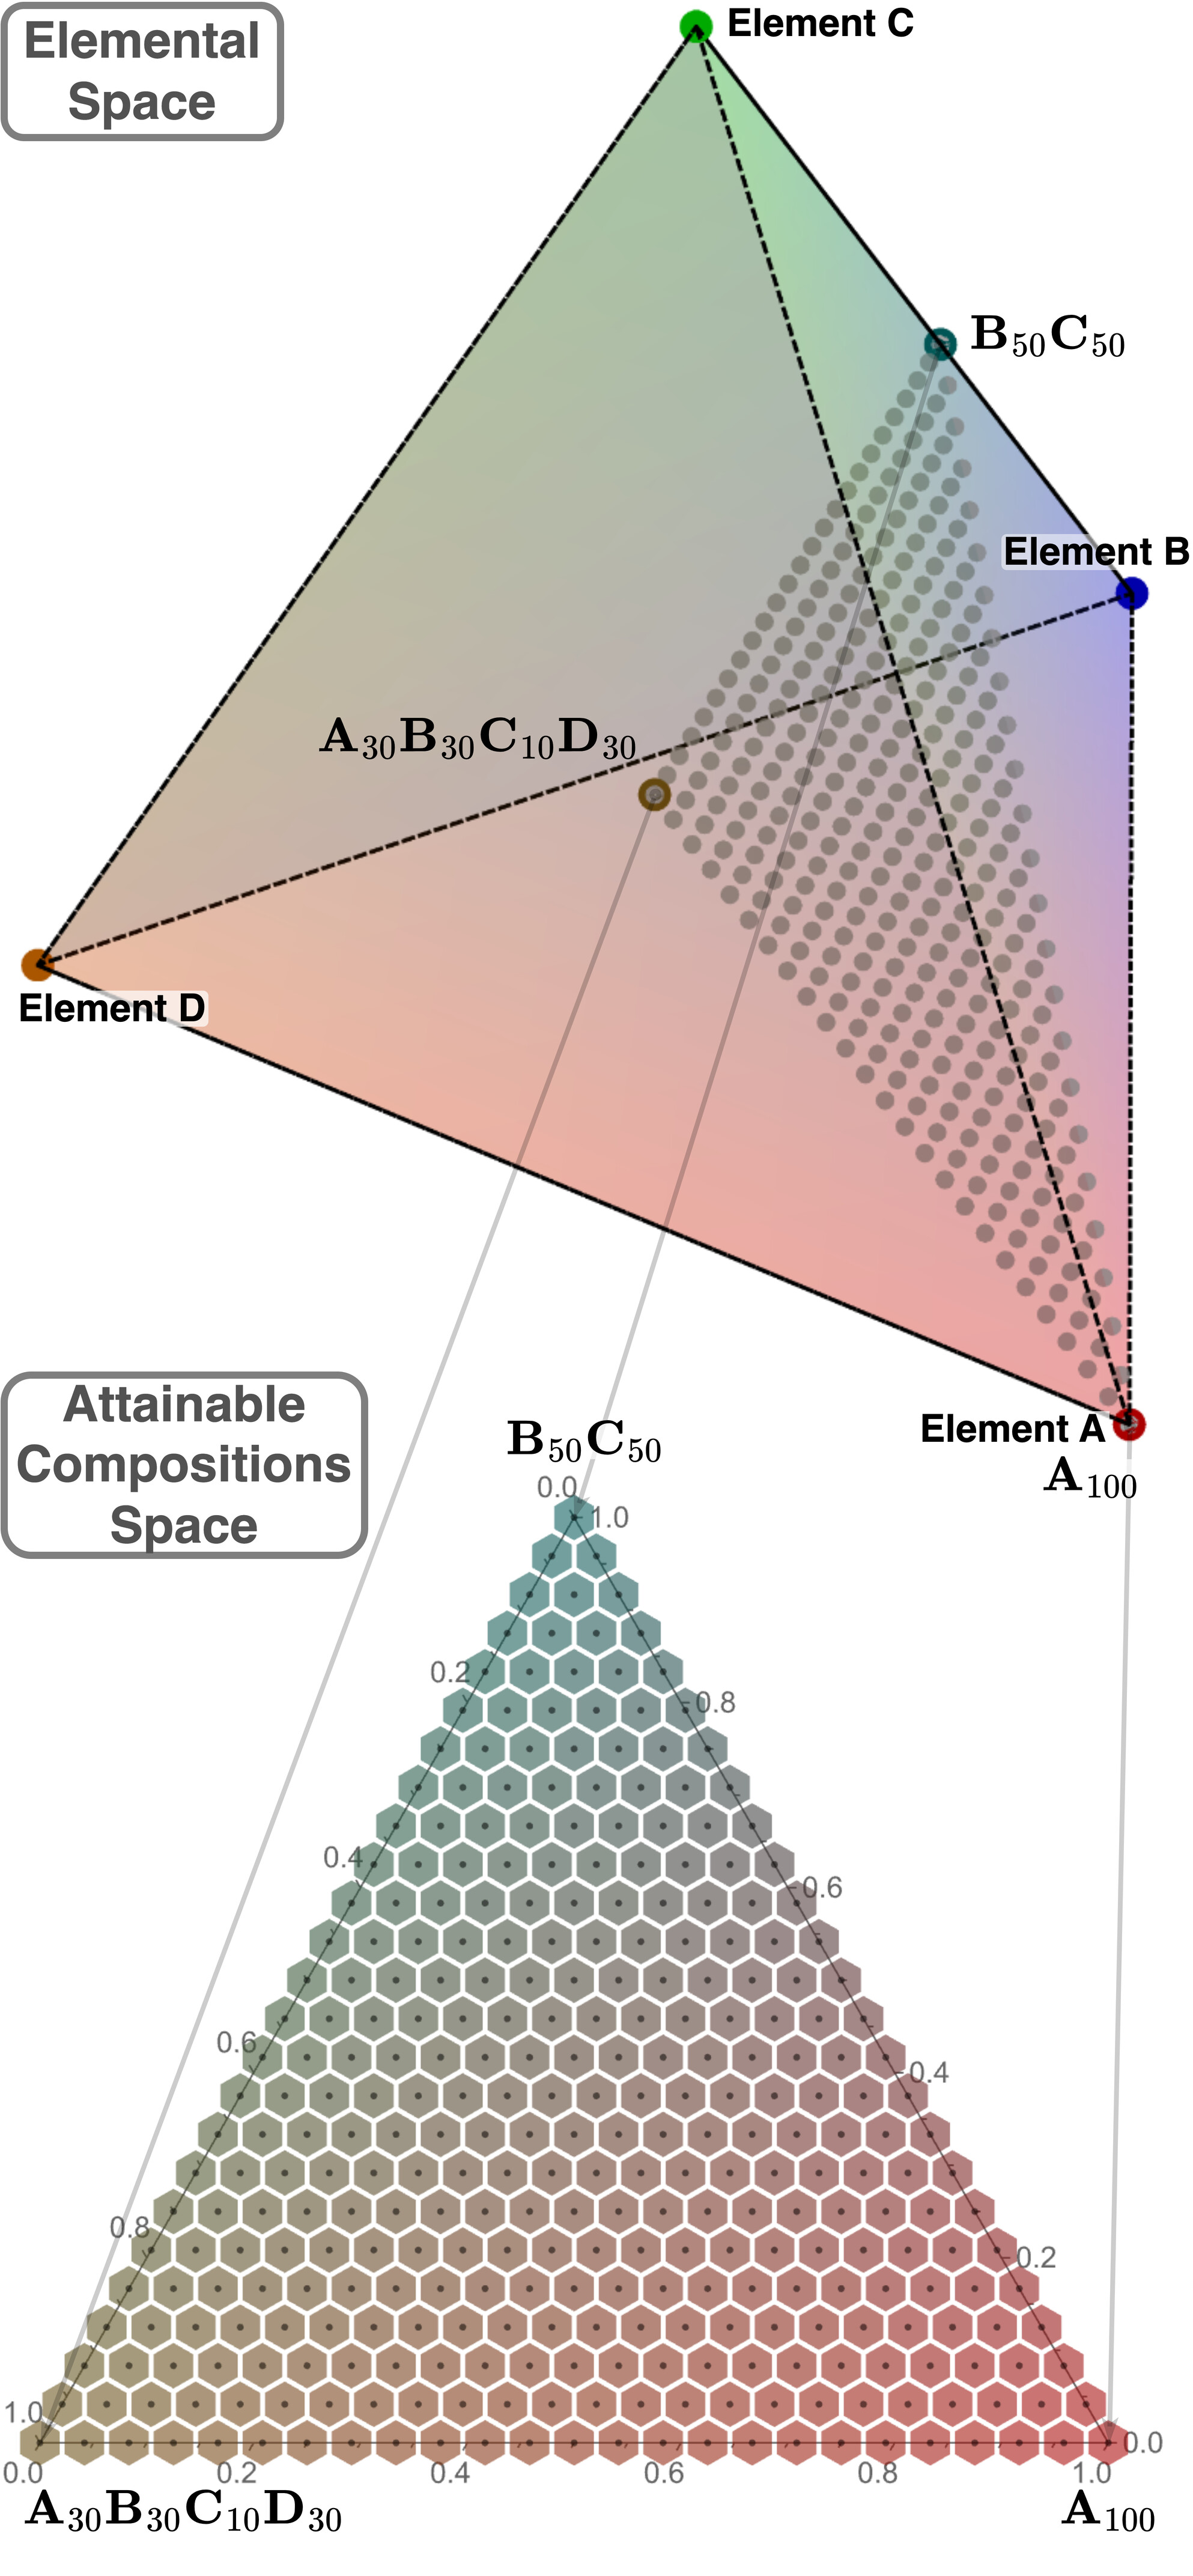
\includegraphics[width=0.38\textwidth]{nimplex/Spaces.png}
    \caption{Three available compositions existing in a quaternary (d=4) compositional space forming a ternary (d=3) compositional space which can be attained with them; sampled with a uniform grid with 24 divisions. The hexagonal tiling emerges based on the distance metric in 2-simplex and would become rhombic dodecahedral in 3-simplex.} 
    \label{nimplex:fig:fgmspaces}
\end{figure}

While in recent years, the fabrication of FGMs has become dominated by Directed Energy Deposition AM for various geometries (e.g., radial deposition \cite{Hofmann2014DevelopingManufacturing}), several other notable manufacturing techniques allow the deployment of such pathways. These include deposition-based methods for high-precision applications, casting-based methods for high-volume fabrication \cite{Saleh202030Challenges}, and recently, brazing consecutive metallic foils \cite{Wu2023ATechnology} to create relatively thin compositionally graded interfaces on mass.

In a typical FGM manufacturing scenario, a discrete set of compositions (individual available materials) exists in a compositional (simplex) space formed by a union of all components (usually chemical elements or compounds - not affecting later steps), as depicted in the top of Figure~\ref{nimplex:fig:fgmspaces}, which one could call the \emph{elemental space}. The position in this elemental space is fundamental and is usually the one considered in both mechanistic (e.g., thermodynamic CALPHAD-type models \cite{Olson2023GenomicDynamics}) and predictive (ML/empirical-rule) modeling. However, during the FGM design, it is more convenient to consider another compositional space formed by treating the original available compositions as components, as depicted on the bottom of Figure~\ref{nimplex:fig:fgmspaces}, which one could call \emph{attainable compositions space} or more generally the \emph{design space}.


Within an FGM manufacturing apparatus, it is common for each of the available compositions to be treated equally, e.g., powder hoppers \cite{Reichardt2021AdvancesMaterials}, sputtering targets \cite{Wu2023ATechnology}, or other flow sources are symmetrically arranged and offer the same degree of control. Thus, as depicted in Figure~\ref{nimplex:fig:fgmspaces}, the attainable compositional space can be treated as a standard simplex for design purposes and partitioned equally across dimensions, reflecting the nature of the problem even though equidistant points in it may not be equidistant in the original (elemental) space.

The attainable spaces used in the final design tend to be lower-dimensional relative to the corresponding elemental spaces, especially when the available compositions are CCMs/HEAs or the number of flow sources is limited. However, this trend is not fundamentally required, and going against it may be beneficial in many contexts. For instance, one may conceptualize a ternary ($d=3$) elemental compositional space where 4 compositions are available, arranged as vertices of some tetragon; thus, forming a quaternary ($d=4$) attainable compositions space tetrahedron. In such a case, some regions have to overlap in the elemental space, while new regions are guaranteed to be unlocked relative to 3 available compositions if the formed tetragon is strictly convex. This seemingly oversamples; however, it is critical to consider that there is no oversampling in the design space because the available materials can possess properties that are not a function of the composition alone, such as the $CO_2$ footprint or price. 

A clear and industry-significant example of the above happens during FGM design in elemental spaces containing Hf and Zr. The two are very difficult to separate, causing both price and greenhouse emissions to rise sharply as a function of the separation purity requirements. Furthermore, physical form factors available from suppliers tend to be limited or at lower demand for pure-Zr and pure-Hf, furthering the cost. In 
the case of AM using wires as feedstock (WAAM) \cite{Shen2016FabricationProcess}, as explored in detail in Section \ref{nimplex:app1}, using pure Zr in place of the more industry-common alloy with $4.5\%$Hf can be somewhere from a few times to over 100 times more expensive. In a typical, manual FGM design, a researcher selects one of the two grades based on their expertise. However, by considering the two grades as independent components of the higher-dimensional design space, one can avoid forcing a decision before exploring the space, thus limiting human bias and allowing exploration of both options simultaneously, allowing their combination where regions of space insensitive to the Hf content utilize the cheaper grade while the pure Zr is used when necessary or favorable based on some path heuristic.

\begin{figure}[H]
    \centering
    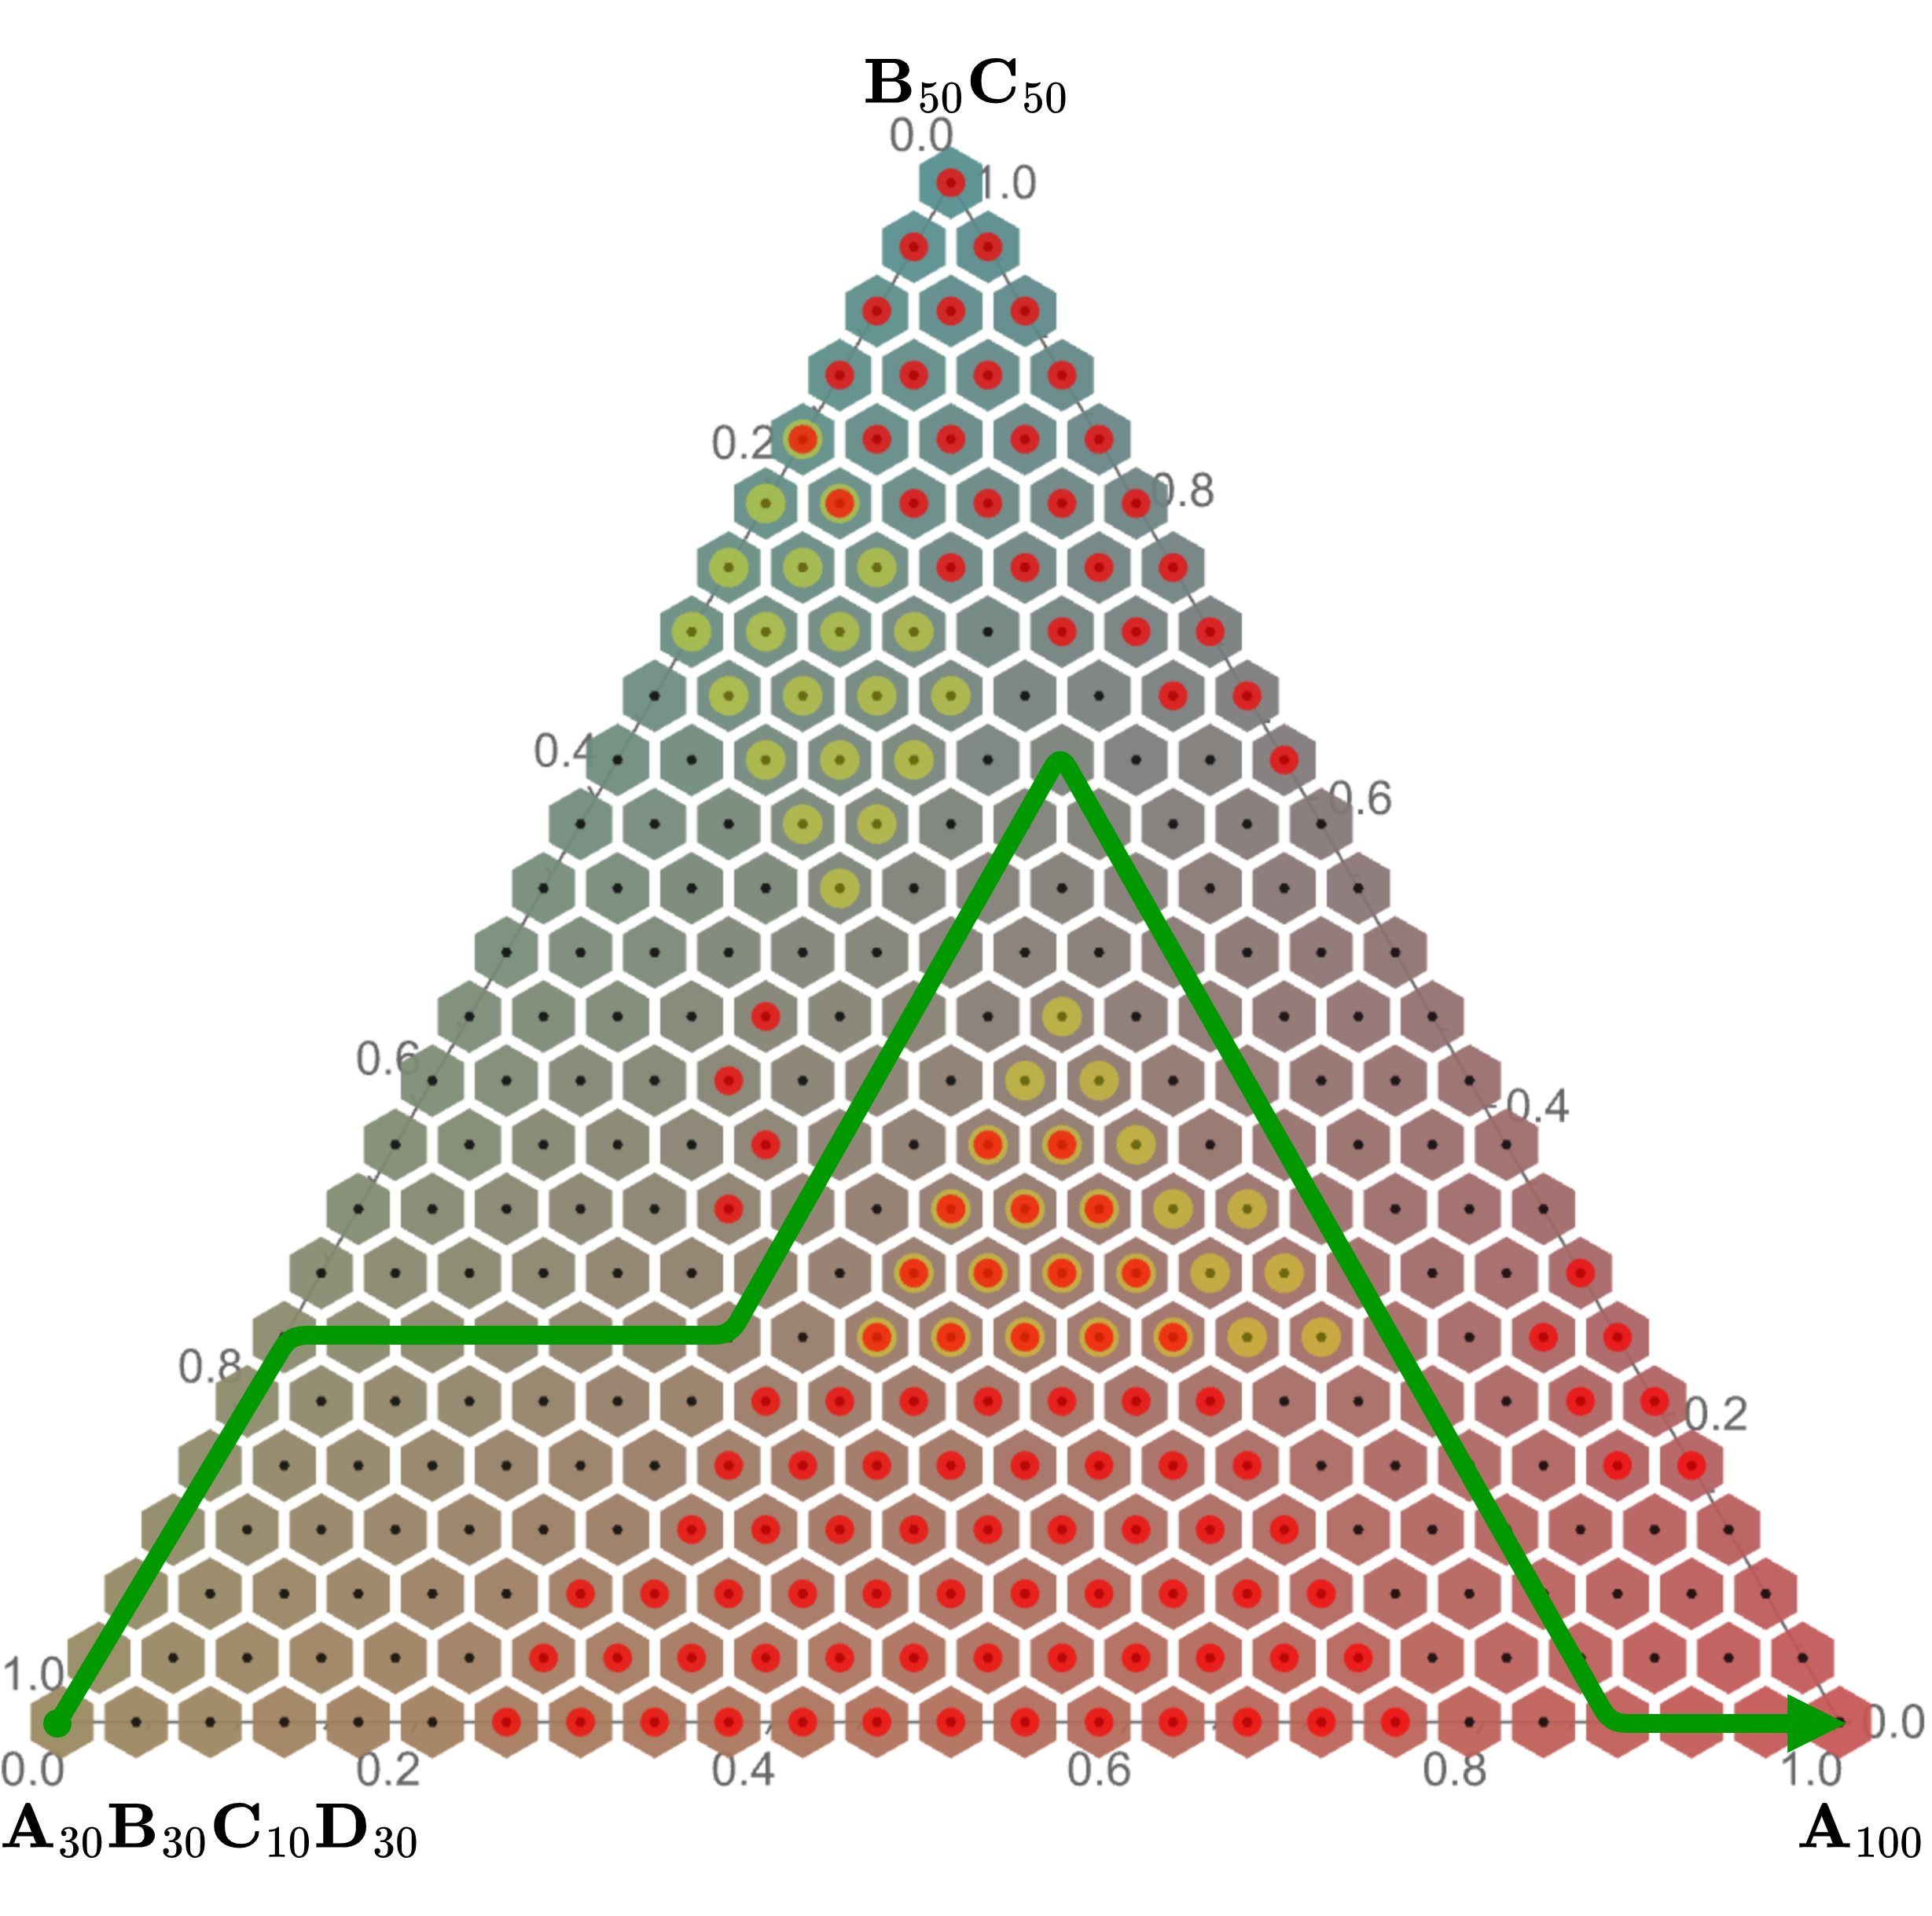
\includegraphics[width=0.475\textwidth]{nimplex/PathPlanning_1.png}
    \vspace{-6pt}
    \caption{A path example which avoids infeasible (red) and undesirable (yellow) regions, or their combination (orange).} 
    \label{nimplex:fig:pathplanning1}
\end{figure}

With the design space carefully set up, one can start to evaluate different paths across it. Typically, the core considerations deal with meeting specific feasibility (hard) constraints. In the case of metal alloy FGMs, these can be (1) formation of detrimental phases based on thermodynamic equilibrium \cite{Reichardt2021AdvancesMaterials}, (2) formation of detrimental phases based on non-equilibrium predictions of solidification results based on Scheil–Gulliver method, which better describes the as-made material \cite{Bocklund2020ExperimentalMaterials}, or (3) a combination of the two \cite{Bobbio2022DesignCompositions}. In the future, these will likely be extended through (4) precipitation modeling improving the metastable material design, thanks to the recent release of open-source high-performance software Kawin \cite{Ury2023Kawin:Model}, and (5) automated modeling of manufacturing constraints, such as printability in AM \cite{SheikhAnAlloys}. Furthermore, one can also try to meet desirability (soft) constraints, such as the physical appearance of a composite material, which can be broken if needed. These two types of constraints are depicted in Figure~\ref{nimplex:fig:pathplanning1}, alongside an example path navigating through them.

In Figure~\ref{nimplex:fig:pathplanning1}, all infeasible points violating the constraints are annotated for visualization. However, doing so may be unnecessary when path-planning, especially iteratively based on neighbor connectivity, as the insides of the infeasible space could not be reached, thus reducing the total number of evaluations. 


In addition to the feasibility and desirability constraints, further considerations are often made to how the path optimizes values of a set of properties of interest, either individually or through some heuristics combining them. Usually, this optimization constitutes finding the path that minimizes or maximizes either average or extreme values over the set of visited states, exemplified by the pink path in Figure~\ref{nimplex:fig:pathplanning2}. In the case of metal alloy FGMs, this can mean, for instance, minimizing the average evaporation rate of the molten metal \cite{Mukherjee2016PrintabilityManufacturing}, minimizing the maximum susceptibility to different cracking mechanisms \cite{Yang2023DesignCracking}, or maximizing the ductility \cite{Hu2021ScreeningAlloys}.

\begin{figure}[H]
    \centering
    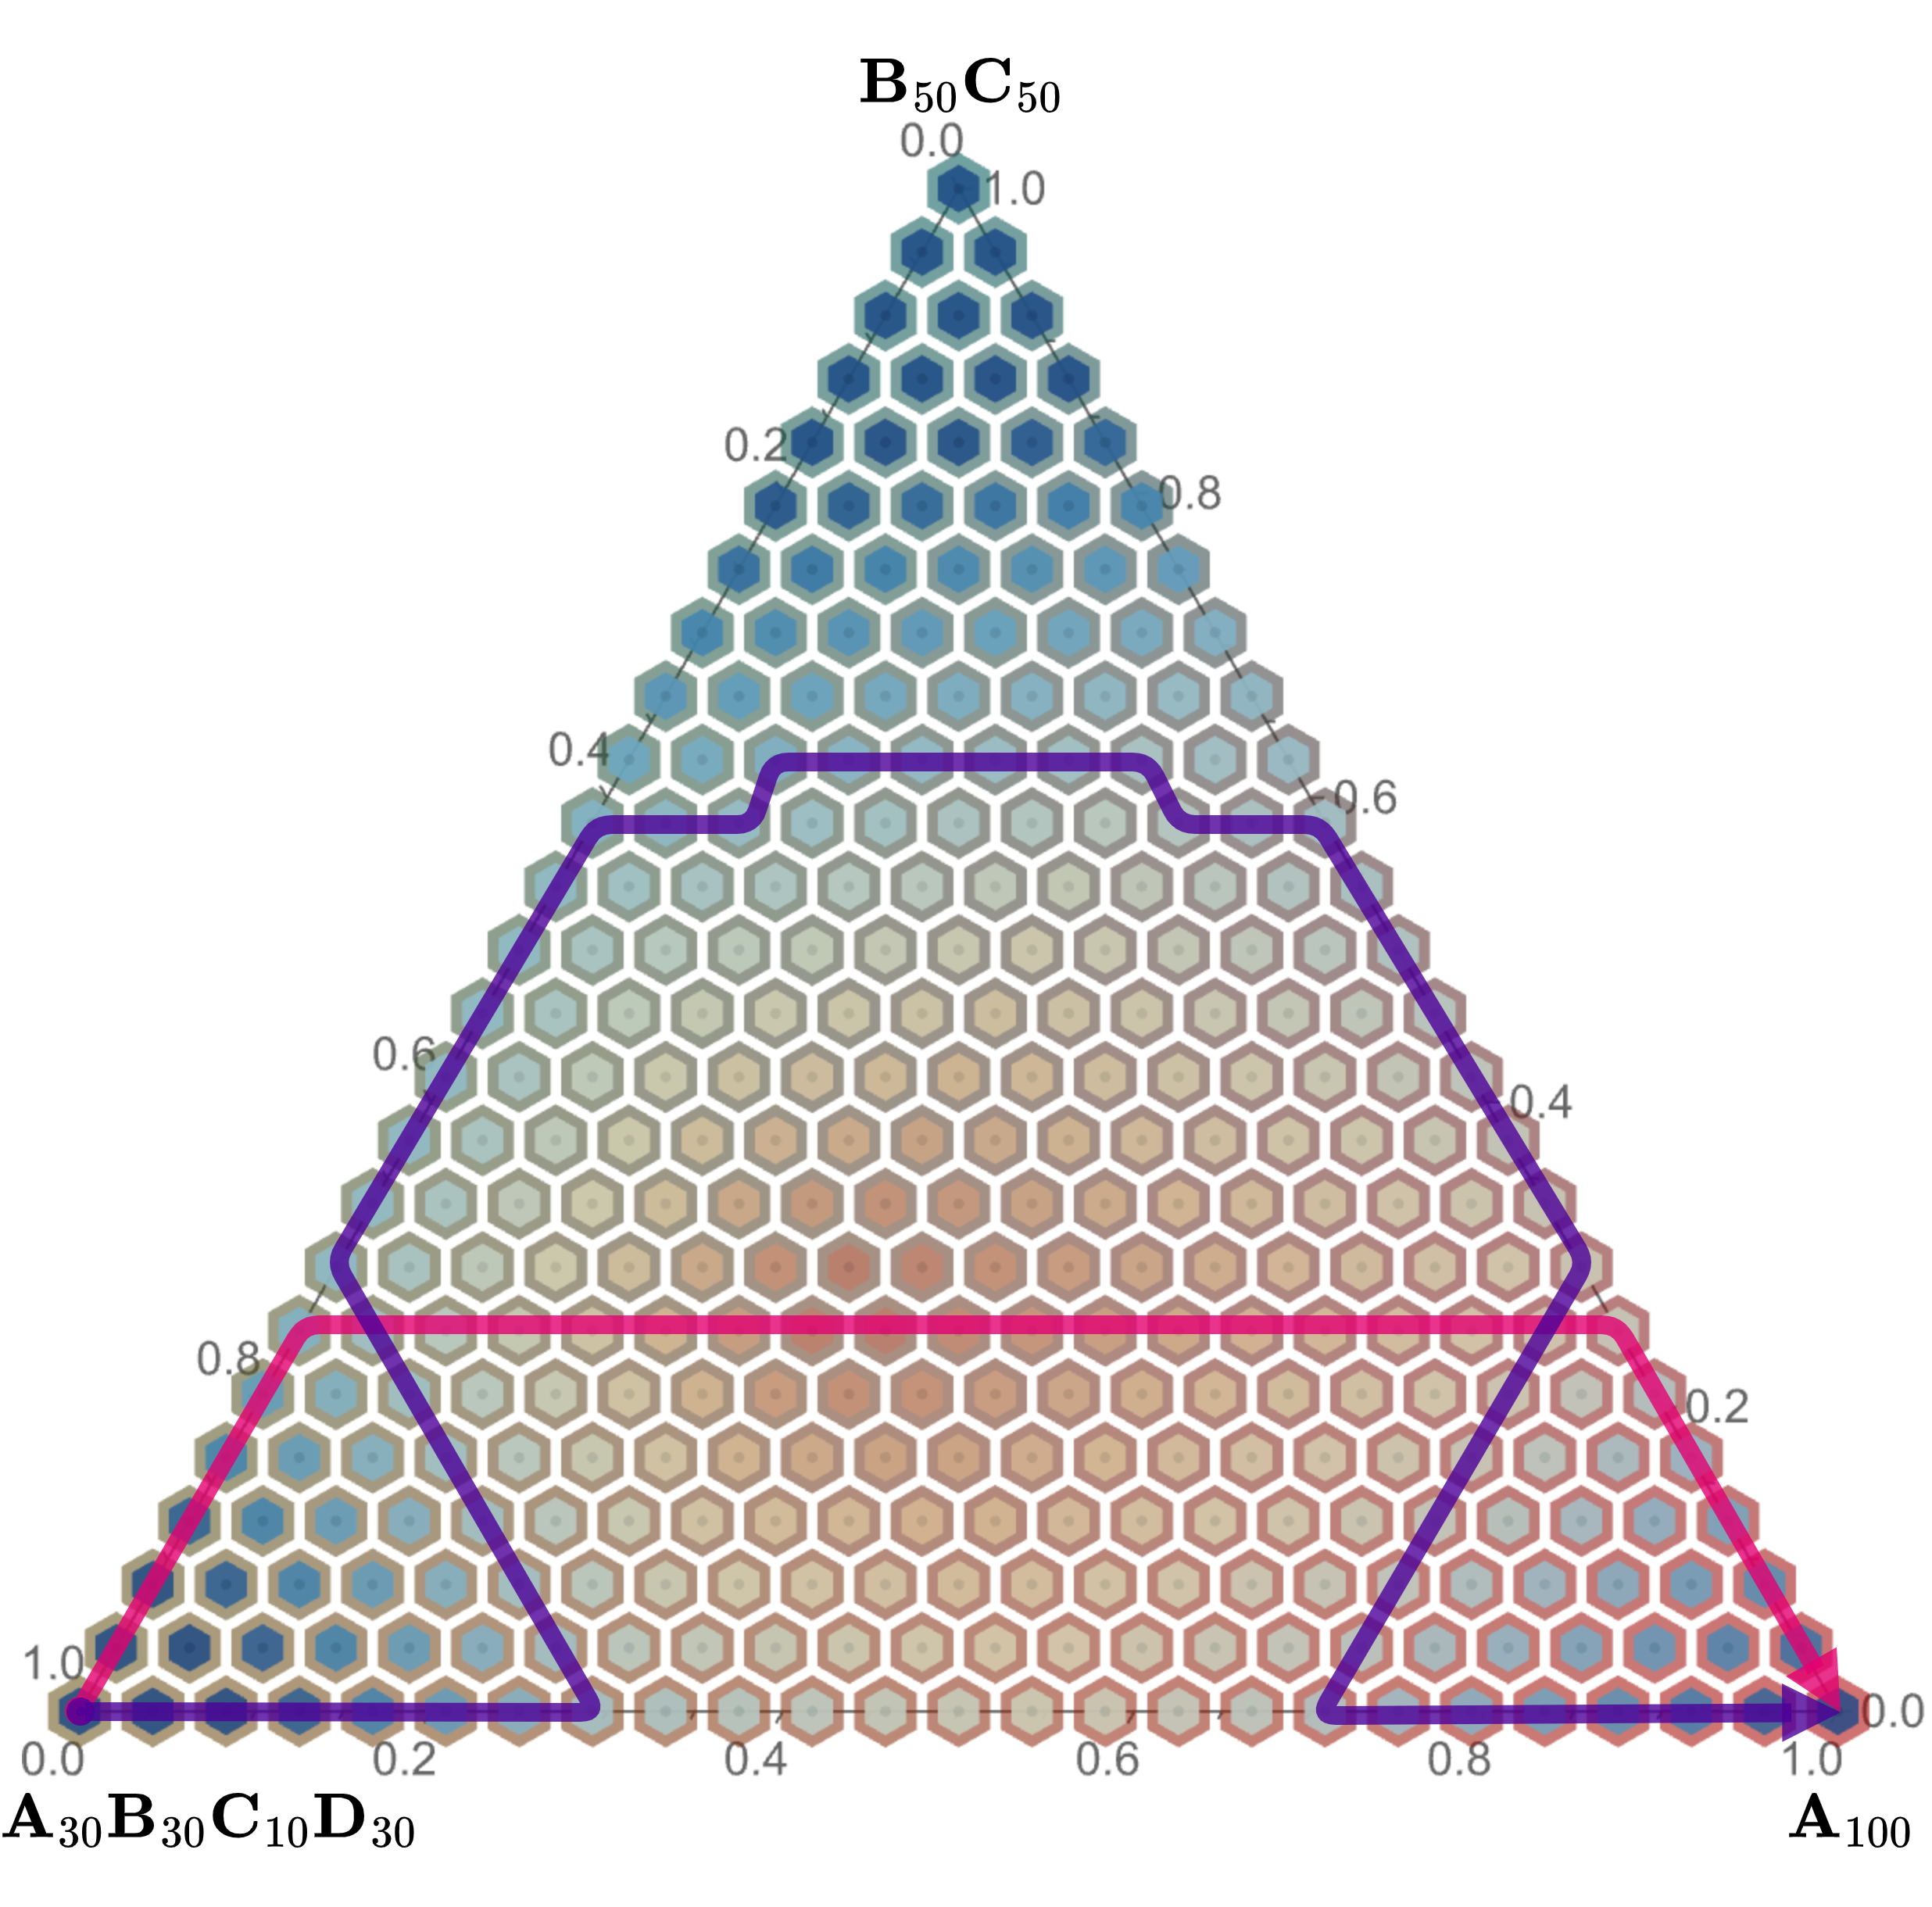
\includegraphics[width=0.475\textwidth]{nimplex/PathPlanning_2.png}
    \caption{Two path examples in the attainable compositional space annotated with some virtual property. One (pink/inner) minimizes/maximizes the average property value given a number of fixed path lengths, and another (purple/outer) minimizes the gradient in the property along the path.} 
    \label{nimplex:fig:pathplanning2}
\end{figure}

The last, fundamentally different, property optimization task has to do with the gradient, or more generally, the character, of transitions between intermediate states, which will be critical later in the context of graphs in Section~\ref{nimplex:sec:simplexgraph}. Most commonly, one optimizes the path to minimize value function gradients, exemplified by the purple path in Figure~\ref{nimplex:fig:pathplanning2}, in order to, for instance, minimize the thermal expansion coefficient mismatch and by extension stresses induced by temperature changes \cite{Kirk2021ComputationalMonotonicity}.



\subsection{Combinatorial Complexities} \label{nimplex:ssec:combinatorialcomplexities}

As eluded to in Sections~\ref{nimplex:ssec:compositionallycomplex} and \ref{nimplex:ssec:functionallygraded}, when sampling compositions or partitioning corresponding spaces, the resulting combinatorial complexities have to be considered to determine whether a method will be computationally feasible. There are two key equations governing these complexities based on (1) the dimensionality of the space (number of components) $d$ and (2) the number of equal divisions made in each dimension $n_d$, which can be found for every feasible fractional step size (such that it can add to $100\%$). 

The first, very intuitive equation gives the number of samples $N_C$ on a Cartesian grid in $d-1$ dimensions, with $-1$ term due to one of the components being considered dependent.
\begin{equation}
    N_C(d, n_d) = (n_d+1)^{d-1}
    \label{nimplex:eq:nc}
\end{equation}
The second equation gives the number of ways $n_d$ balls can be arranged in $d$ bins, which is well known to be equivalent to much simpler problems of choosing $d-1$ moves or $n_d$ placements from $d-1+n_d$ possible options (see \cite{Nijenhuis1978CombinatorialCalculators} or \cite{Chasalow1995AlgorithmPoints}). While these may seem unrelated to compositions, the former problem is precisely equivalent to finding a composition of an integer or distributing $n_d$ compositional fractions $\frac{1}{n_d}$ across components or chemical elements, giving the number $N_S$ of unique discrete compositions in the simplex space.
\begin{equation}
    N_S(d, n_d) = \binom{d-1+n_d}{d-1} = \binom{d-1+n_d}{n_d}
    \label{nimplex:eq:ns1}
\end{equation}
In terms of factorials, both expressions can be simplified to the same
\[N_S(d, n_d) = \frac{(d - 1 + n_d)!}{(d-1)!n_d!}\]
Throughout Sections~\ref{nimplex:sec:simplexgrid}~and~\ref{nimplex:sec:simplexgraph}, the interplay between these equations will be utilized to contrast different computational methods, and their direct results will allow computational feasibility evaluation. 


\section{Simplex Uniform Random Sampling} \label{nimplex:sec:randomuniformsampling}

\subsection{Monte Carlo} \label{nimplex:ssec:mc}

Performing a uniform random sampling, also known as the Monte Carlo method, over a simplex space is a prevalent task; however, it is also one of the most common sources of inefficiency, bias, or errors when implemented incorrectly.

Software (e.g., \texttt{alchemyst/ternplot} in Matlab \cite{Sandrock2017Alchemyst/ternplothttps://github.com/alchemyst/ternplot}) and methods dealing with low-dimensional or otherwise small compositional spaces, often utilize a na\"ive approach of sampling uniformly distributed points from a Cartesian space/grid in $d-1$ dimensions and then rejecting some infeasible points ($\sum^d_i x_i > 1$), as depicted in the left part of Figure~\ref{nimplex:fig:samplinginternary}, which for small ($d \leq 4$) can be both easiest and computationally fastest. 

However, this method becomes inefficient for large $d$ because the fraction of rejected points increases with the dimensionality. While this problem is widely noted in the literature \cite{Allen2022AAlloys}, best to the authors' knowledge, it has yet to be discussed quantitatively despite being critical to estimating the sampling's computational complexity. Thus, it is derived herein.

One can consider that a grid of $N_S$ simplex-feasible points is a subset of a grid of $N_C$ points distributed uniformly in the Cartesian space so that random selection from this grid should have a $\frac{N_S}{N_C}$ probability of falling within the simplex. Thus, as shown below, one can find the acceptance rate by considering an infinitely fine grid ($n_d\rightarrow\inf$). Section \ref{nimplex:app2} gives an alternative, intuitive method for finding $f(4)$ using geometry, which agrees with this result.

\begin{equation}
    \begin{aligned}
        f(d) &= \lim_{n_d\rightarrow\inf} \frac{N_S}{N_C} = \lim_{n_d\rightarrow\inf} \frac{\binom{d-1+n_d}{d-1}}{(n_d+1)^{d-1}}\\
        &= \Gamma(d)^{-1} = \frac{1}{(d-1)!} = \frac{d}{d!}
    \end{aligned}
    \label{nimplex:eq:fd}
\end{equation}
As one can see in Equation~\ref{nimplex:eq:fd}, the rejection rate exhibits factorial growth, and while it is not a significant obstacle for low-dimensional cases like ternary $f(3)=\frac{1}{2}$ or a quaternary $f(4) = \frac{1}{6}$, it will relatively quickly become a problem when compositionally complex materials are considered. For instance, in the case of nonary chemical space $f(9) = \frac{1}{40320}$ or only $\approx0.0025\%$ of points will fall into the feasible space. Such a rejection rate could have a particularly severe effect on ML-driven methods, such as generative CCM design.

\begin{figure}[h]
    \centering
    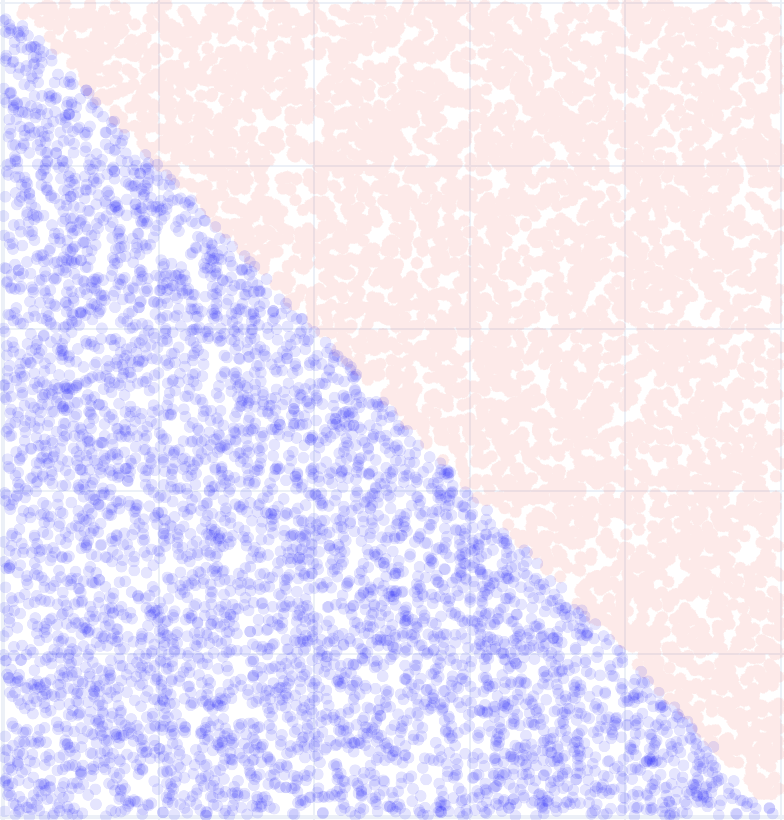
\includegraphics[width=0.270\textwidth]{nimplex/1A.png}
    \hfill
    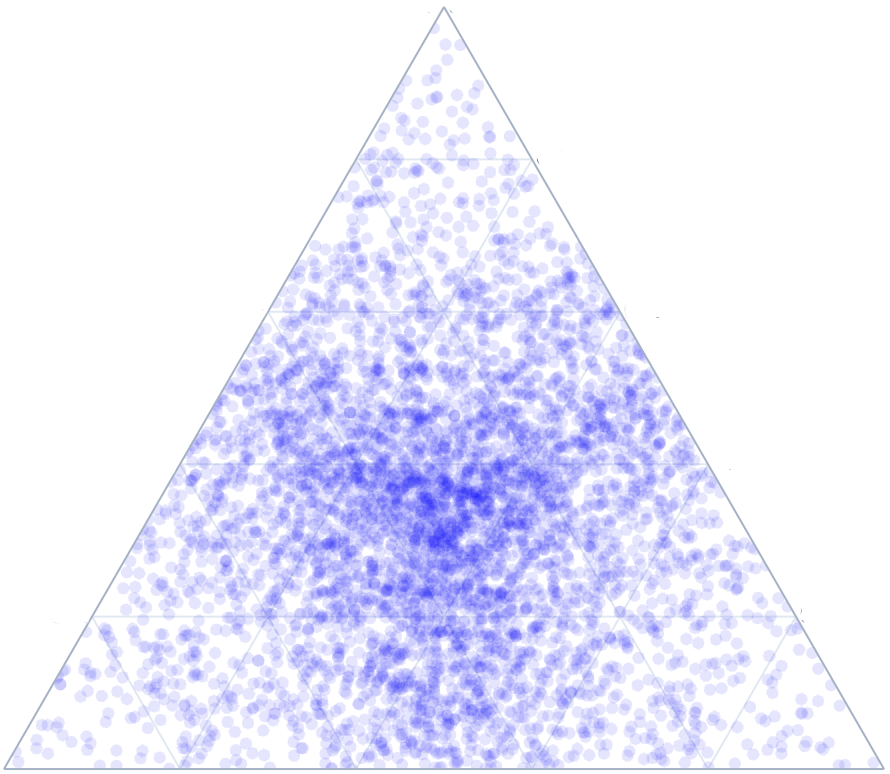
\includegraphics[width=0.320\textwidth]{nimplex/1C.png}
    \hfill
    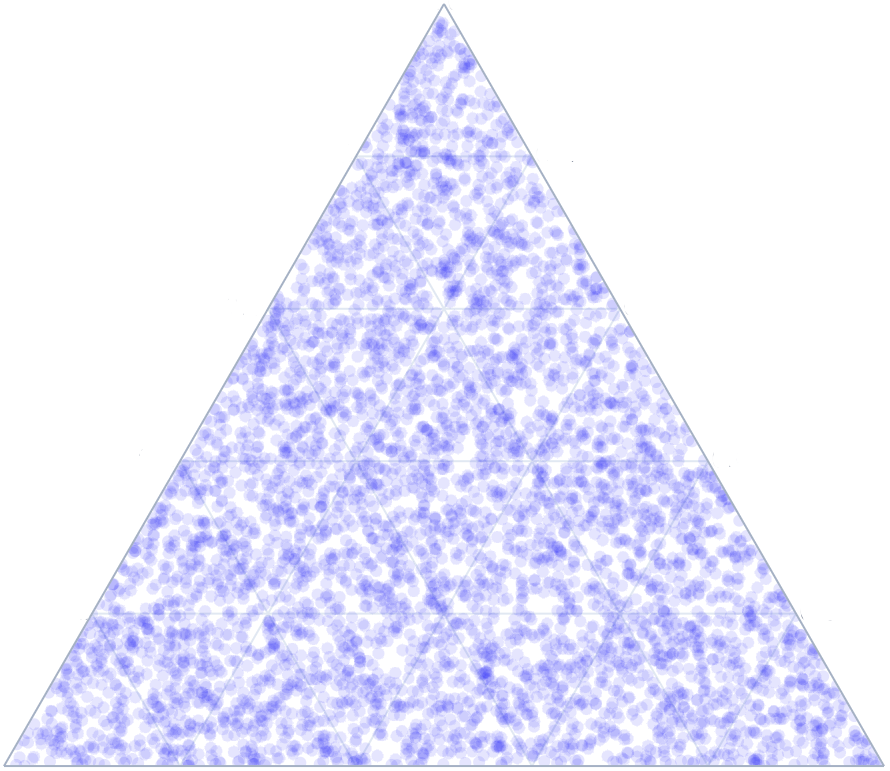
\includegraphics[width=0.320\textwidth]{nimplex/1B.png}
    \caption{(left) Uniform random sampling in 2-cube (square) filtered to fall onto a 2-simplex (ternary composition), showing 50\% rejection rate, (middle) random sampling in 3-cube projected onto 2-simplex by normalizing coordinates, showing oversampling in the center of each dimension, and (right) ideal uniform random sampling of a simplex.} 
    \label{nimplex:fig:samplinginternary}
\end{figure}

To circumvent the rejection problem, one may randomly sample from N-cube and normalize to 1; however, as shown in the center of Figure~\ref{nimplex:fig:samplinginternary} and commonly known in the literature \cite{Otis2017AnSystems}, this leads to oversampling in the center of each underlying dimension.

Thus, to achieve a uniform random sampling, \texttt{nimplex} and other carefully designed methods (e.g., \cite{Allen2022AAlloys} and \cite{Otis2017AnSystems}) tend to take Dirichlet distribution, where one samples points $\textbf{y}$ from Gamma distributions with density $\frac{y_i^{\alpha-1} e^{-y_i}}{\Gamma(\alpha)}$ and consider its special "flat" case, where $\alpha=1$ simplifies the density equation to just $\frac{1 e^{-y_i}}{1} = e^{-y_i}$. This is equivalent to sampling $\textbf{z}$ from linear distributions and calculating $y_i=-\log(z_i)$, which then can be normalized to obtain $\textbf{x}$ as $x_i = y_i / \sum \textbf{y}$. The following snippet shows \texttt{nimplex}'s implementation of this, which samples \textbf{z} with the high-performance \texttt{xoroshiro128+} random number generator \cite{Blackman2018ScrambledGenerators} underlying \texttt{randomTensor} function from the \texttt{Arraymancer} tensor library \cite{RatsimbazafyMratsim/Arraymancer:Backends}.

\begin{minted}[xleftmargin=3\parindent, linenos=true, mathescape]{nim}
proc simplex_sampling_mc(dim: int, samples: int): Tensor[float] =
  let neglograndom = 
    randomTensor[float]([samples, dim], 1.0
    ).map(x => -ln(x))
  let sums = neglograndom.sum(axis=1)
  return neglograndom /. sums
\end{minted}

An alternative approach worth mentioning, sometimes found in this context, is based on (1) generating a $(d+1)$-length list composed of $0$, $d-1$ random numbers, and $1$, (2) sorting it, and (3) obtaining $d$-length list of differences between consecutive elements, which is guaranteed to be uniformly distributed over a simplex as shown in \cite{Rubin1981TheBootstrap}. While this approach may be easier to conceptualize, it is much more computationally expensive due to the sorting step. On the author's laptop, for $d=9$, the method implemented in \texttt{nimplex} (involving calculation of 9 logarithms and normalizing them) takes $3.6$ns while the above (implemented with merge sort) takes $74.5$ns per iteration, i.e., over 20 times longer while not providing any clear benefit. Furthermore, their complexities are $\mathcal{O}(N)$ and $\mathcal{O}(N \ln N)$, respectively, so the computational cost difference will also slowly widen with increasing $d$. 


\subsection{Quasi Monte Carlo} \label{nimplex:ssec:qmc}
While beyond the current implementation scope of \texttt{nimplex}, it is beneficial to consider quasi-Monte Carlo (QMC) sampling methods, where quasi-random sequences of low discrepancy (having highly uniform coverage of all regions) are used to sample the space deterministically. Such an approach is guaranteed to be very beneficial in low-dimensional ($d\leq3$) problems and has been implemented in thermodynamic tools, including \texttt{pycalphad} \cite{Otis2017Pycalphad:Python, Otis2017AnSystems} improving sampling of ternary systems. However, the QMC can become problematic as one moves to higher dimensional problems. 

Firstly, the upper discrepancy bounds for QMC quickly increase with increasing $N$, unlike MC, which depends only on the number of samples; thus, MC \textit{can} outperform it (thanks to better guarantees) unless a quickly (often exponentially) growing number of samples is taken (see discussion on p.271 in \cite{Asmussen2007StochasticAnalysis}). Because of this, even for quaternary ($d=4$) spaces, MC may be preferred for a low number of samples, even though QMC, especially with additional scrambling, \textit{can} outperform it, as shown in \cite{Otis2017AnSystems}. 

Another significant problem in QMC is the unequal sampling of different dimensions, which can be very severe in high dimensions (see p.154 in \cite{Lemieux2009MonteSampling}). In addition to causing under-performance in space-filling, such bias, combined with the standard alphabetical ordering of chemical components, can cause systematically worse exploration of, e.g., titanium compared to aluminum in CCMs, just based on their names.


\section{Simplex Grid} \label{nimplex:sec:simplexgrid}

\subsection{Full} \label{nimplex:ssec:fullgrid}

Next, one can consider the creation of a grid of uniformly distributed points, which is known to contain $\binom{d-1+n_d}{d-1}$ points, as discussed in Section~\ref{nimplex:ssec:combinatorialcomplexities}. Similar to the random sampling discussed in Section~\ref{nimplex:sec:randomuniformsampling}, such a compositional grid cannot be constructed by simply projecting a Cartesian grid in $(N-1)$-cube as patterns will emerge (explored in detail in \cite{Otis2017AnSystems}), but it can be quickly constructed through rejecting infeasible points, as shown in Figure~\ref{nimplex:fig:simplexgrid}. However, it will suffer from a nearly as bad rejection rate, quantitatively dependent on both $d$ and $n_d$. For instance, if we consider $5\%$ spaced compositions in 9-components, the fraction of points summing to $100\%$ is $f_{M=20}(9) \approx \frac{1}{12,169}$ or $0.0082\%$. 

\begin{figure}[h]
    \centering
    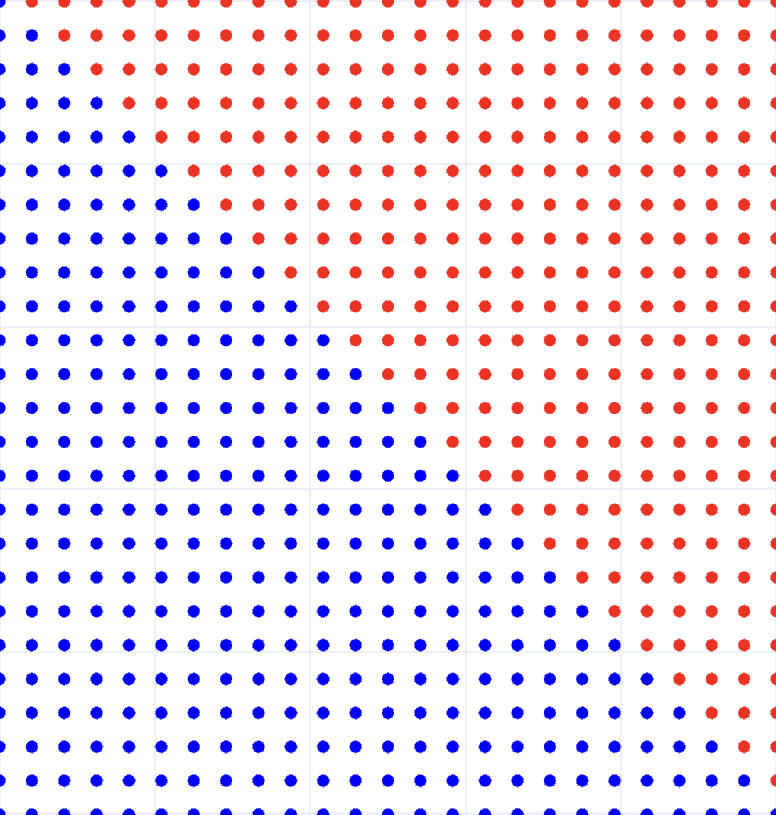
\includegraphics[width=0.270\textwidth]{nimplex/2A.png}
    \hspace{48pt}
    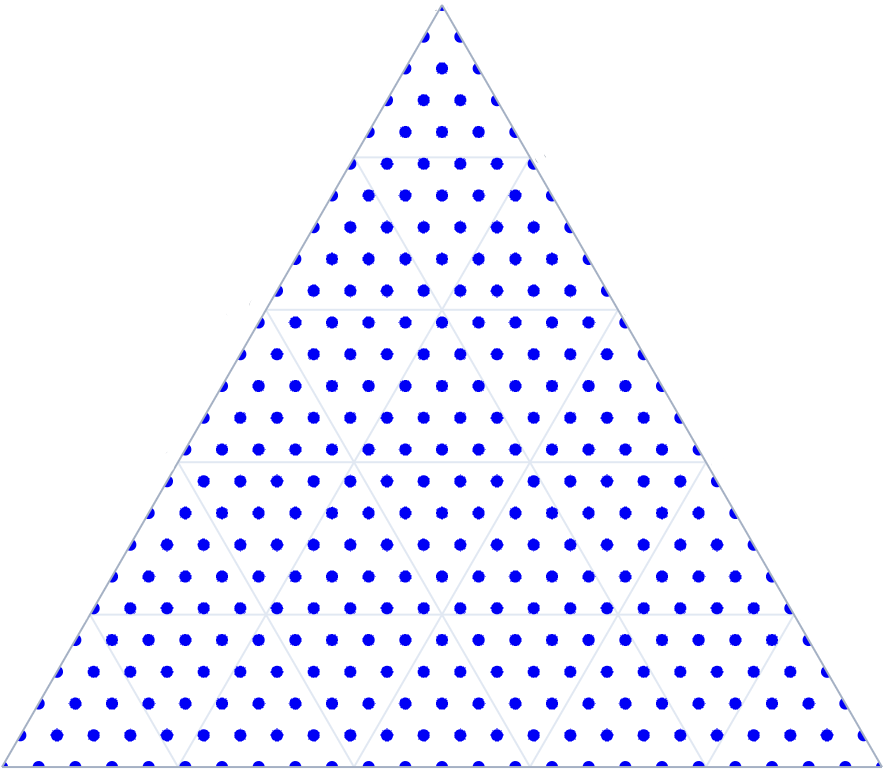
\includegraphics[width=0.320\textwidth]{nimplex/2B.png}
    \caption{(left) Uniform grid ($n_d=24$) in 2-cube (square) filtered to fall onto a 2-simplex (ternary composition), showing $\frac{12}{25}=48\%$ rejection rate, (right) uniform grid in the corresponding simplex.} 
    \label{nimplex:fig:simplexgrid}
\end{figure}

Fortunately, in their 1978 textbook, \citet{Nijenhuis1978CombinatorialCalculators} explored the problem and gave an efficient algorithm/routine called NEXCOM to procedurally generate these simplex lattice points for arbitrary $d$ and $n_d$, resulting in the grid shown in Figure~\ref{nimplex:fig:simplexgrid} on the right.

In the following years, several authors made various modifications to the algorithm, and the most recent one by \citet{Chasalow1995AlgorithmPoints} improves performance without sacrificing simplicity. Over the years, it has been implemented in relatively modern languages such as FORTRAN90, C, MATLAB, and Python. Now, it has been implemented in Nim language as well, with the Nim code snippet shown below.

\begin{minted}[xleftmargin=3\parindent, linenos=true, mathescape]{nim}
proc simplex_grid(dim: int, ndiv: int): Tensor[int] =
  let N: int = binom(ndiv+dim-1, dim-1)
  result = newTensor[int]([N, dim])
  var x = zeros[int](dim)
  x[dim-1] = ndiv
  for j in 0..dim-1:
    result[0, j] = x[j]
  var h = dim
  for i in 1..N-1:
    h -= 1
    let val = x[h]
    x[h] = 0
    x[dim-1] = val - 1
    x[h-1] += 1
    for j in 0..dim-1:
      result[i, j] = x[j]
    if val != 1:
      h = dim
  return result
\end{minted}

As one can deduce from above, the algorithm proceeds through the simplex space starting from $[0, 0, ..., n_d]$ and redistributes one $\frac{1}{n_d}$ fraction $N_S-1$ times across dimensions, forming a zig-zag path to $[n_d, 0, ..., 0]$.

\subsection{Internal} \label{nimplex:ssec:internalgrid}

To the best of the authors' knowledge, something that has not been implemented before, but that is significant to exploration of CCMs  (see Sec \ref{nimplex:ssec:compositionallycomplex}) is an algorithm to obtain only internal points of the simplex grid, i.e., points with non-zero values in all dimensions, to allow, e.g., generating all 7-component HEAs rather than all alloys in 7-component space. In principle, one can filter the output of the algorithm presented in Section~\ref{nimplex:ssec:fullgrid}; however, this may quickly become inefficient, especially for $n_d$ low enough as to approach $d$. 

The number of points can be found by, again, considering the surrogate problem of ball compositions mentioned in Section~\ref{nimplex:ssec:combinatorialcomplexities} and noting that if the last ball cannot be removed from any position, there will be $d$ fewer possible options to perform $d-1$ moves, thus resulting in $N_I$ samples:
\begin{equation}
    N_I(d, n_d) = \binom{n_d-1}{d-1}
\end{equation}
This can be quickly double-checked through summation of internal points of all lower $\delta$ dimensional spaces enclosed in $d$ space:
\[\sum_{\delta=1}^d \Biggl[ \binom{n_d-1}{\delta-1} \times \binom{d}{\delta} \Biggr] =  \frac{(d - 1 + n_d)!}{(d-1)!n_d!} = N_S(d, n_d)\]
We can now look at $N_I(d, n_d)$ to $N_S(d, n_d)$ ratio for the aforementioned case of generating all 7-component alloys. For $5\%$ grid ($n_d=20$) we get $\approx \frac{1}{8.5}$, and for $10\%$ grid ($n_d=10$) we get $\approx \frac{1}{95}$, showing a clear benefit of implementing the new method. This can be done by taking the modified-NEXCOM algorithm \cite{Chasalow1995AlgorithmPoints} from Section~\ref{nimplex:ssec:fullgrid} and:
\begin{enumerate}
    \item Adjusting procedure length from $N_S$ to $N_I$.
    \item Initializing first states in \textbf{x} to 1.
    \item Adjusting the starting point from [1, 1, ..., $n_{div}$] to [1, 1, ..., $n_{div}-d_{im}+1$].
    \item Jumping to the next dimension one step earlier ($val \neq 2$).
\end{enumerate}

To implement the following \texttt{nimplex} snippet.

\begin{minted}[xleftmargin=3\parindent, linenos=true, mathescape]{nim}
proc simplex_internal_grid(dim: int, ndiv: int): Tensor[int] =
  let N: int = binom(ndiv-1, dim-1)
  result = newTensor[int]([N, dim])
  var x = ones[int](dim)
  x[dim-1] = ndiv+1-dim
  for j in 0..dim-1:
    result[0, j] = x[j]
  var h = dim
  for i in 1..N-1:
    h -= 1
    let val = x[h]
    x[h] = 1
    x[dim-1] = val - 1
    x[h-1] += 1
    for j in 0..dim-1:
      result[i, j] = x[j]
    if val != 2:
      h = dim
  return result
\end{minted}


\section{Simplex Graph} \label{nimplex:sec:simplexgraph}

The simplex grid algorithm presented in Section~\ref{nimplex:ssec:fullgrid} is used commonly; however, it has an important feature that has not been utilized yet and was only briefly noted by its authors \cite{Chasalow1995AlgorithmPoints}. Namely, the fact that generated points are sorted in a lexicographic order (forward or reverse, depending on convention) which opens the door for using pure combinatorics for finding certain interesting relations between points at near-zero costs compared to other popular methods.

\subsection{Binary} \label{nimplex:ssec:binarygraph}

In the simplest possible case, which will be expanded upon later, one can look at a binary ($d=2$ / 1-simplex) compositional grid and write a straightforward function that will find all neighboring points (\emph{transitions} to them) to create a graph representation of the binary system like one presented in Figure~\ref{nimplex:fig:binarysimplexgraph}, without any notion of distance calculations.

\begin{figure}[H]
    \centering
    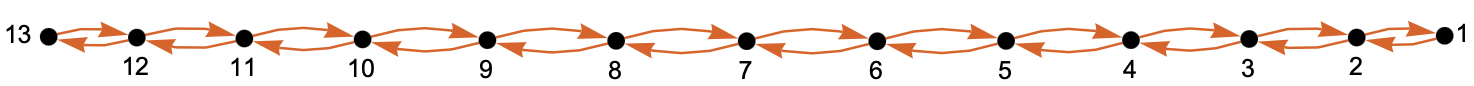
\includegraphics[width=0.55\textwidth]{nimplex/SimplexGraphBinary.png}
    \caption{1-simplex graph corresponding to a binary system ($n_d=12$) with 13 nodes/compositions and 24 edges/transitions.} 
    \label{nimplex:fig:binarysimplexgraph}
\end{figure}

Such a function, shown below, can be implemented by setting up a \texttt{neighbors} list of lists ($N_S$ of $\leq2$ length) of integer positions and then, at the end of every $i$-th iteration, populating it with forward ($i+1$) and backward ($i-1$) transitions unless start ($[0,1]$) or end ($[1,0]$) points $\textbf{x}$ respectively, corresponding to lack of some component, have been reached.


\begin{minted}[xleftmargin=3\parindent, linenos=true, mathescape=true]{nim}
proc neighborsLink2C(
    i:int, x:Tensor, neighbors: var seq[seq[int]]): void =
  if x[0] != 0:
    neighbors[i].add(i+1)
  if x[1] != 0:
    neighbors[i].add(i-1)
\end{minted}

While the above is trivial, it clearly demonstrates that the graph can be constructed within the original $\mathcal{O}(N)$ computational complexity of the simplex grid algorithm, unlike a similarly trivial distance matrix calculation, which would be $\mathcal{O}(N^2)$; thus, unlocking efficient generation of even massive graphs of this kind.

\subsection{Ternary} \label{nimplex:ssec:ternarygraph}

With the core of the approach set up in Section~\ref{nimplex:ssec:binarygraph}, one can move to the more complex ternary ($d=3$  / 2-simplex) case, which can be conceptualized as a series of $13$ binary systems (already solved individually in Sec. \ref{nimplex:ssec:binarygraph}) of lengths from $13$ to $1$ and with simple modification of positional coordinates shifted forward by 1 to accommodate for the new dimension. 

The newly allowed neighbor transitions across these binaries can be quickly noticed to be dependent on which of these binaries is considered; however, they can be intuitively found by considering that each transition in the 3rd dimension (increasing $x_0$) limits the size of the binary simplex by 1 from the original size of $\binom{d-1+n_d}{d-1} = \binom{2-1+n_d}{2-1} = n_d+1$. Thus, one can define two convenient jump lengths:
\[
\begin{aligned}
    J_0^{d=3} &= 1\\
    J_1^{d=3}(x_0) &= 1 + n_d - x_0
\end{aligned}
\]
Then, one can quickly visualize that (1) unless $x_2=0$, a transition by jump $J_1$ should be possible, (2) unless $x_1=0$, a transition by jump $J_1$ combined with backward jump $J_0$ in the target binary should be possible, and (3) unless $x_0=0$ (the first traversed binary is considered), transitions by both backward jump $J_1$ and backward jump $J_1+J_0$ (extra step within the earlier binary) should be possible. Thus, one arrives at the following algorithm, which requires additional $n_d$ ("ndiv") input on top of the one from Section~\ref{nimplex:ssec:binarygraph} but retains its structure.

\begin{minted}[xleftmargin=3\parindent, linenos=true, mathescape=true]{nim}
proc neighborsLink3C(
    i:int, x:Tensor, neighbors: var seq[seq[int]], ndiv: int): void =
  let jump0 = 1
  let jump1 = 1+ndiv-x[0]
  if x[0] != 0:
    neighbors[i].add(i-jump1)
    neighbors[i].add(i-jump1-jump0)
  if x[1] != 0:
    neighbors[i].add(i-jump0)
    neighbors[i].add(i+jump1-jump0)
  if x[2] != 0:
    neighbors[i].add(i+jump0)
    neighbors[i].add(i+jump1)
\end{minted}

Utilizing the above, the result presented in Figure~\ref{nimplex:fig:ternarysimplexgraph} can be quickly obtained for any number of divisions. The numbering of points can help to visualize how the transitions were obtained.

\begin{figure}[h]
    \centering
    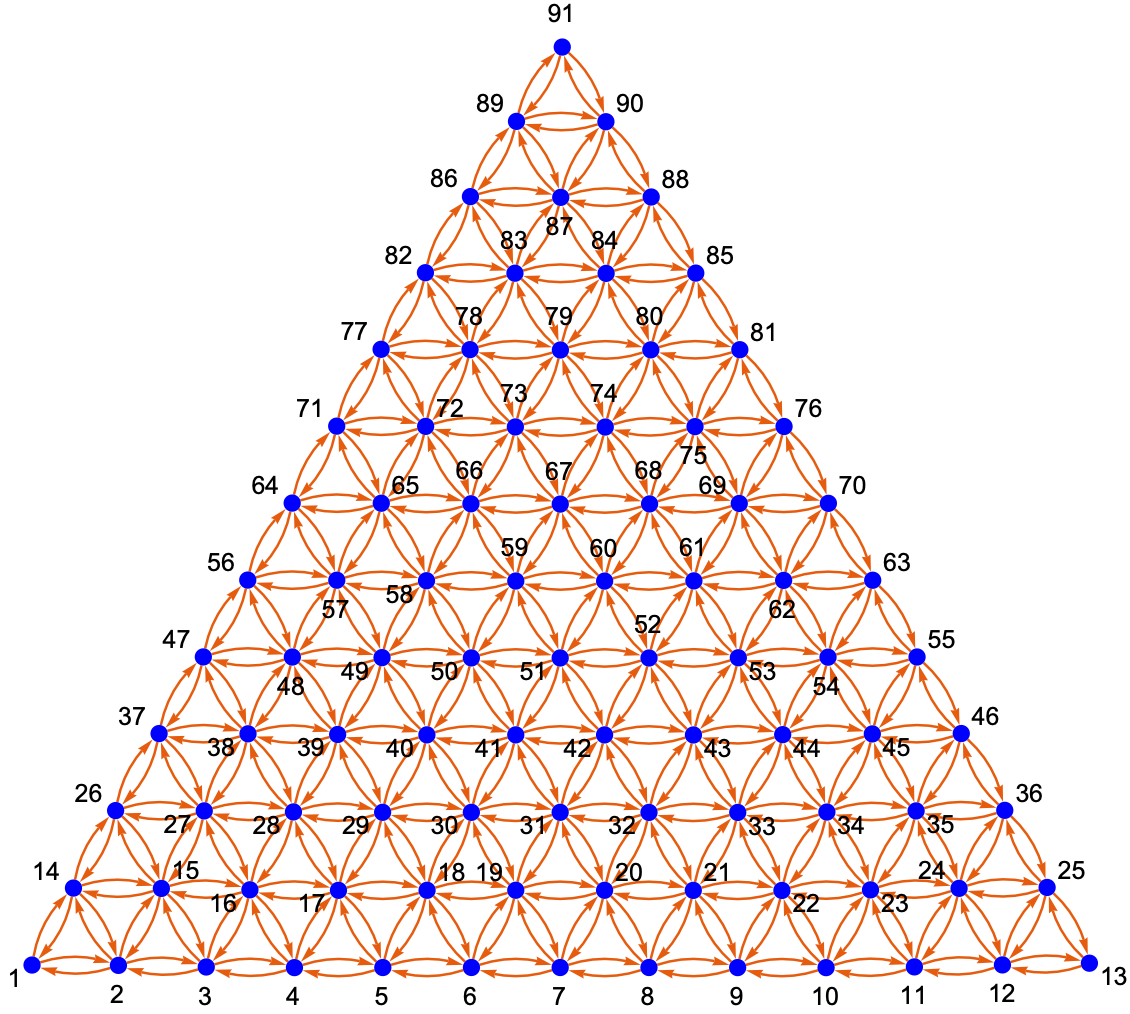
\includegraphics[width=0.55\textwidth]{nimplex/SimplexGraphTernaryBlue.png}
    \caption{2-simplex graph corresponding to a ternary system ($n_d=12$) with 91 nodes/compositions and 468 edges/transitions.} 
    \label{nimplex:fig:ternarysimplexgraph}
\end{figure}

\subsection{N-Dimensional} \label{nimplex:ssec:ndimgraph}

Moving beyond ternary systems, one has to increase the number of tracked transitions to higher dimensions, which can be counted for every jump length $J_j$ with $\sum_0^{(d-j-2)}x_i$, and then utilized to obtain a general equation for all $d-1$ elements of jump length array $\textbf{J}$ as a function of current point $\textbf{x}$.
\begin{equation}
    J_{j}(\textbf{x})= \binom{j+n_d- \sum_{i=0}^{(d-j-2)} x_i}{j}
    \label{nimplex:eq:jj}
\end{equation}
As expected, for the special cases of $d=3$, the above agrees with $J_0$ and $J_1$ found for the ternary case in Section~\ref{nimplex:ssec:ternarygraph}. One can also note that $J_0$ always equals to $1$ as $\binom{a}{0} = 1$ for any $a$.

With $\textbf{J}$ defined, one can take a quaternary system (d=4 / 3-simplex) and perform a similar visualization thought exercise in the head as in Section~\ref{nimplex:ssec:ternarygraph}, but in 3D, considering the new transitions to 3 neighbors above and 3 neighbors below, in order to set up \texttt{\textbf{neighborsLink4C}} procedure which is presented in Section \ref{nimplex:app3}. 

Such an approach of visualizing and counting the possible jumps in the head becomes (a) challenging for quinary systems (d=5 / 4-simplex) case where one has to visualize 4 forward and 4 backward jumps to and from points inscribed in every tetrahedron formed by the 3-simplex tetrahedral grids, and (b) near impossible for higher orders, both because of the visualization dimensionality and the growing number of neighbors to track, given by $\sum_\delta^d 2(\delta-1)= d(d+1)$ or for $d=$ 6, 7, 8, and 9 corresponding to 30, 42, 56, and 72 neighbors respectively; thus prompting for an alternative.

Fortunately, while performing the above thought exercises for increasing $d$, with transition lengths \textbf{T} expressed as compositions of jump lengths described by \textbf{J}, a careful observer can quickly note that for any dimensionality of the simplex grid, the main challenge in finding the higher-dimensional \textbf{T} lies in distributing the $d-1$ new forward ($x_0$ increment) transitions across all previous $x_i=0$ constraints, while the $d-1$ new backward ($x_0$ decrease) transitions are always possible for $x_0>0$ and follow a relatively simple trend of transition lengths $J_d$, $\sum_{j=d-1}^{d}J_j$, ..., $\sum_{j=0}^{d}J_j$. This allows a relatively simple construction of all backward transitions by stacking them together across all $d-2$ considered dimensions. 

Finally, a simple notion that every backward transition $b \rightarrow a$ of grid point $b$ is associated with a forward transition $a \rightarrow b$ of point $a$ allows for the complete construction of the simplex graph representation of the compositional space.

This is implemented very concisely in the \texttt{nimplex} snippet below, where for every considered dimension $\delta$ from $d$ (highest at $0$th index of $\textbf{x}$) down to $2$ ($(d-2)$th index), the $\delta$ of backward and $\delta$ of forward transitions of lengths $t_k$ are found by iteratively summing jump lengths $J_{\delta}$, $\sum_{j=\delta-1}^{\delta}J_j$, ..., $\sum_{j=0}^{\delta}J_j$, and then used to assign neighborhood.

\begin{minted}[xleftmargin=3\parindent, linenos=true, mathescape=true]{nim}
proc neighborsLink(
    i:int, x:Tensor, neighbors: var seq[seq[int]], ndiv: int): void =
  var jumps = newSeq[int](dim-1)
  jumps[0] = 1     #binom(a,0)=1
  for j in 1..<(dim-1):
    jumps[j] = binom(
    j+ndiv-sum(x[0..(dim-2-j)]), j)
  var trans: int
  for order in 0..(dim-2): 
    trans = 0
    if x[order] != 0:
      for dir in 0..(dim-2-order): 
        temp += jumps[dim-2-order-dir]
        neighbors[i].add(i - trans)
        neighbors[i - trans].add(i)           
\end{minted}

The result of running the above algorithm with $d=4$ and relatively low $n_d$ is shown in Figure~\ref{nimplex:fig:quaternarysimplexgraph} to help visualize neighbor-neighbor transitions despite the overlap when printed in 2D.

\begin{figure}[h]
    \centering
    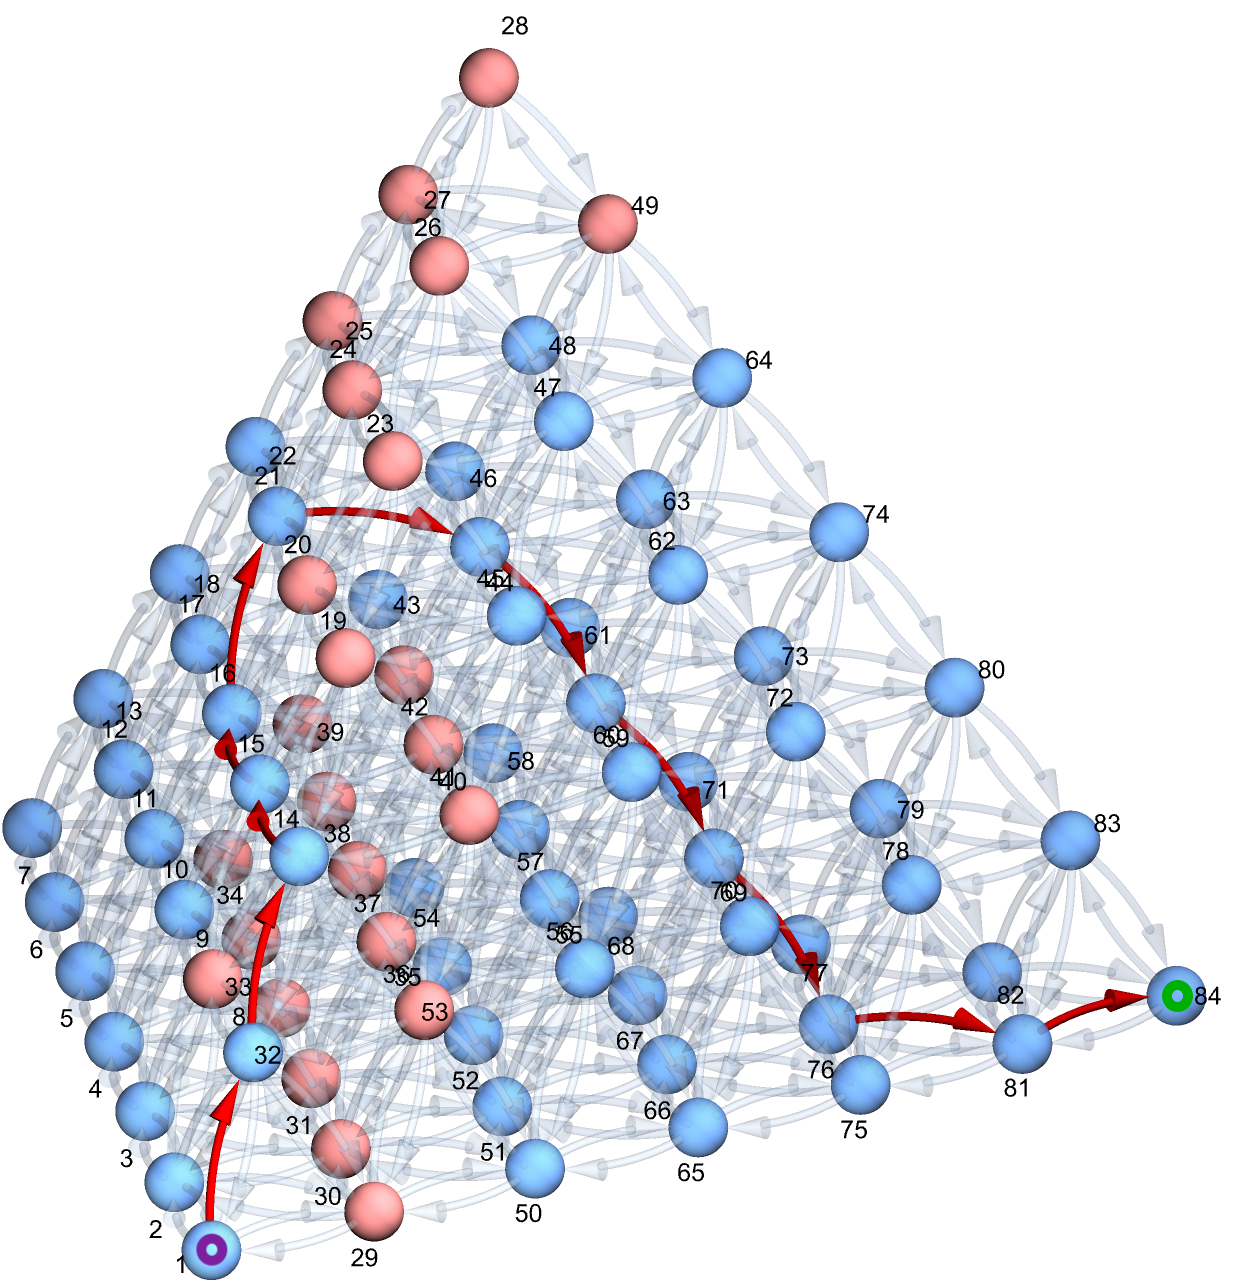
\includegraphics[width=0.6\textwidth]{nimplex/SimplexGraphQuaternaryAnnotated.png}
    \caption{A quaternary (d=4 / 3-simplex) simplex graph ($n_d=6$) with 84 nodes (compositions) and 672 edges (possible moves). A set of nodes has been manually selected (highlighted in pink) to depict a toy example of infeasible points (similarly to Figure~\ref{nimplex:fig:pathplanning1}), which forces a non-trivial path (highlighted in red) to traverse from the bottom-left corner at 1 to the bottom-right corner at 84.} 
    \label{nimplex:fig:quaternarysimplexgraph}
\end{figure}

It is critical to note that the above algorithm is still within the $\mathcal{O}(N)$ computational complexity for $N$ grid points, just like the forward/backward jumps discussed in Section~\ref{nimplex:ssec:binarygraph}. Thus, for instance, the task of constructing 1\% resolution graph for a 6-component chemical space containing $N_S(d=6, n_d=100)$ or nearly \textit{100 million unique vertices} requiring \textit{2.76 billion edges} (possible chemistry changes) takes as little as \textit{23s} tested on author's laptop computer. This stands in stark contrast with $\mathcal{O}(N^2)$ distance-based graph construction, which, even when well implemented to take around $3ns$ per comparison, would take approximately 1 year on the same machine.

Furthermore, the method scales excellently with the increasing problem dimensionality. For a 12-component chemical space with $n_d=12$ divisions per dimension, even though up to $132$ neighbors have to be considered for all $N_S=1.35$ million vertices, the 93 million edges are constructed in 950 milliseconds.


\subsection{Simplex Graph Complexes} \label{nimplex:ssec:complexes}

Once able to rapidly set up simplex graphs in arbitrary dimensions, one can also efficiently combine them to construct more complex graphs representing non-trivial problem statements where many different paths are possible to explore, and prior knowledge can be incorporated as assumptions in the problem solution space if needed. At the same time, it allows the dimensionality of the intermediate compositional spaces to be kept within manufacturing feasibility, i.e., the number of material flow sources.

Suppose one tries to connect elemental compositions A and F, but assumes prior knowledge that they cannot be combined directly in any quantity, and also knows that (1) A is compatible with B and C, (2) F is compatible with D and E, but (3) B and E are incompatible in any quantity, (4) C and D are incompatible in any quantity. Furthermore, (5) G and H are individually compatible with B and D, and (6) I and J are individually compatible with C and E. 

These rules can be used to set up a problem graph like in the top of Figure~\ref{nimplex:fig:graphcomplex1}, encoding everything that is known about the system \textit{a priori} and limiting the solution space from full $\binom{10-1+12}{12} \approx 300,000$ to $2\times\binom{3-1+12}{12} + 10\times\binom{2-1+12}{12} = 312$, or three orders of magnitude.

\begin{figure}[H]
    \centering
    \begin{adjustbox}{valign=c}
        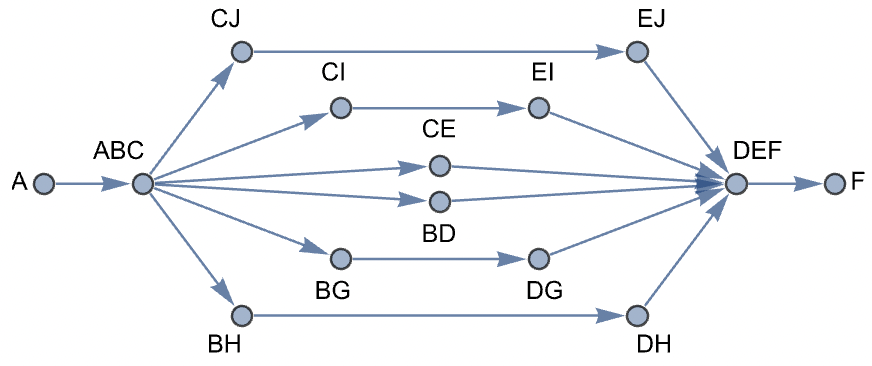
\includegraphics[width=0.45\textwidth]{nimplex/GraphComplexMap1.png}
    \end{adjustbox}
    \hspace{6pt}
    \begin{adjustbox}{valign=c}
        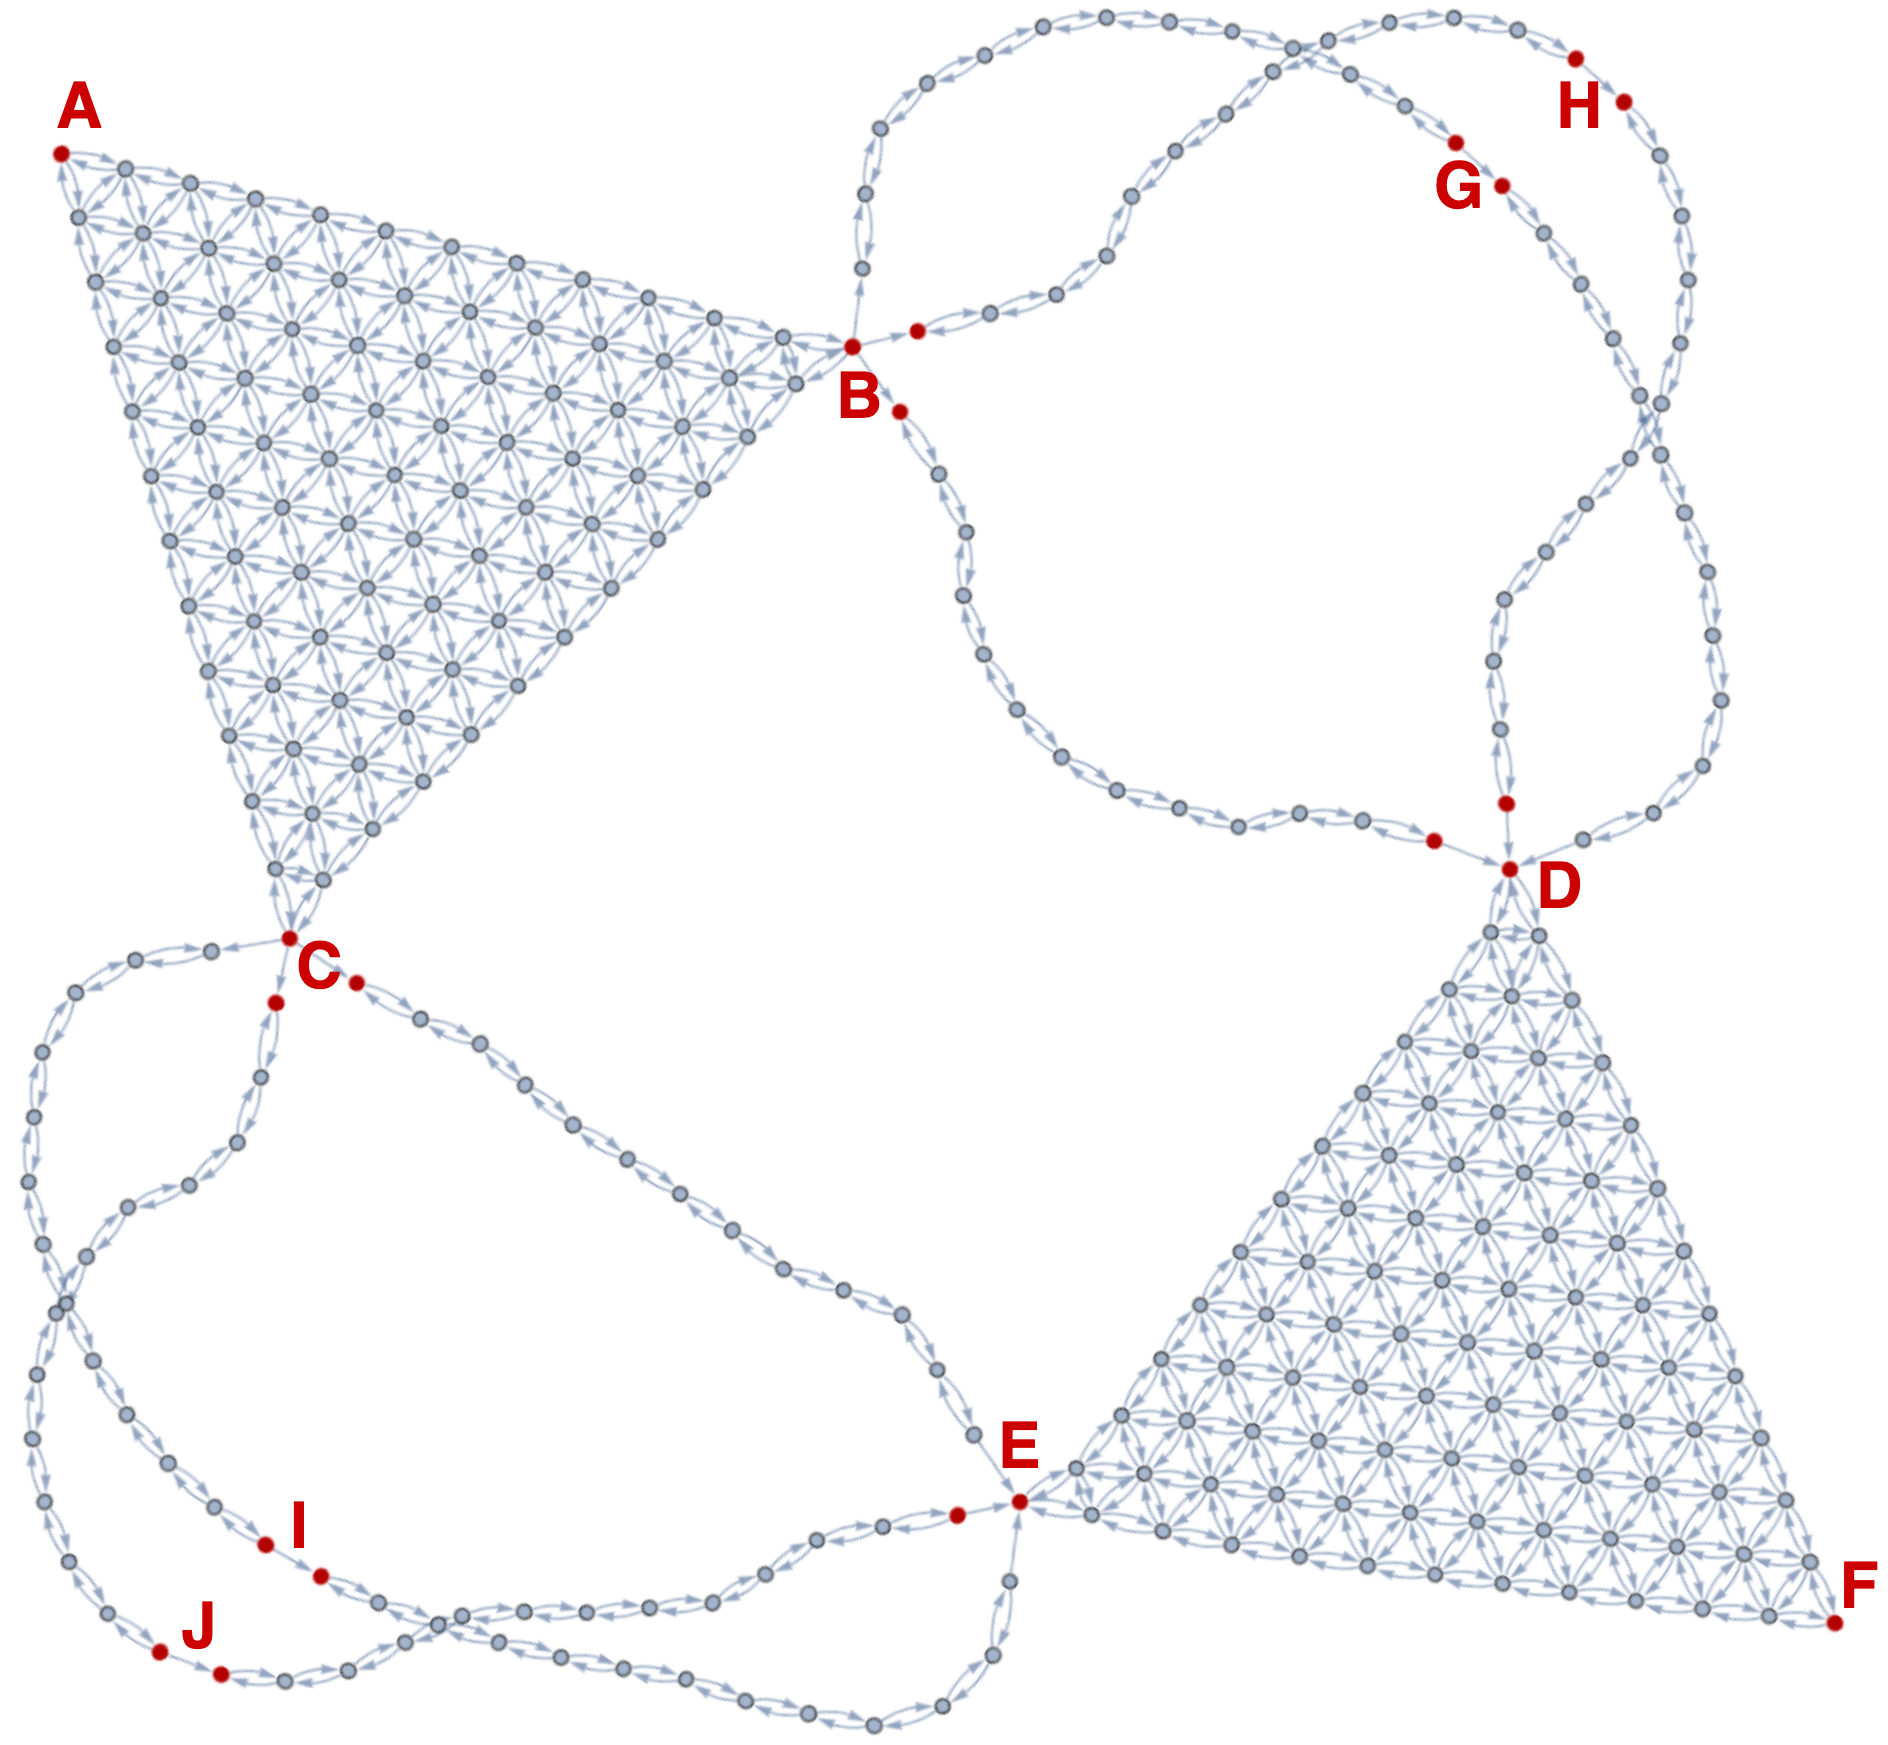
\includegraphics[width=0.5\textwidth]{nimplex/GraphComplex1Trim.png}
    \end{adjustbox}
    \caption{Graph Complex Example \#1 depicting a problem space where 2 ternary systems can be connected through 6 different binary paths.} 
    \label{nimplex:fig:graphcomplex1}
\end{figure}

The space constructed in Figure~\ref{nimplex:fig:graphcomplex1} is kept very minimal in terms of going beyond known assumptions and dimensionality to illustrate the concept in a plane. However, real examples of this technique can be highly non-trivial and essential in bringing the number of considered points into a computationally feasible regime when tens of available compositions can be considered. 

Furthermore, unlike in Figure~\ref{nimplex:fig:graphcomplex1} where spaces are simply connected through single-components, the interfaces between the individual compositional spaces can be along any subspace (e.g., the ternary face of quaternary tetrahedron), allowing one to quickly set up search problems where one or more components are unknown, but their relations to others are fixed. 

One can quickly demonstrate the benefits of such ability by looking at the SS316 to Ti-6Al-4V problem studied by \citet{Bobbio2022DesignCompositions}. After idealizing and anonymizing the components, it becomes a problem where one tries to combine compositions A with G, which cannot be combined directly in almost any quantity, and also knows that (1) system ABC is highly feasible across it, but (2) C cannot be combined directly with G in any quantity, and (3) a complete path from pure B to G is not possible. In this case, a simple problem setup is to look at several BC\texttt{?} and BG\texttt{?} pairs, forming parallel pathways from ABC to G. This is depicted in Figure~\ref{nimplex:fig:graphcomplex2} for 3 candidates D, E, F, forming 6 ternary spaces to consider, but nothing limits the method to be extended to an arbitrary number of candidates while still retaining its linear complexity.

\begin{figure}[h]
    \centering
    \begin{adjustbox}{valign=c}
        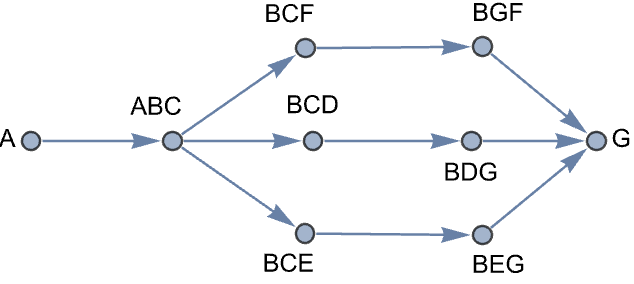
\includegraphics[width=0.37\textwidth]{nimplex/GraphComplexMap2.png}
    \end{adjustbox}
    \hspace{6pt}
    \begin{adjustbox}{valign=c}
        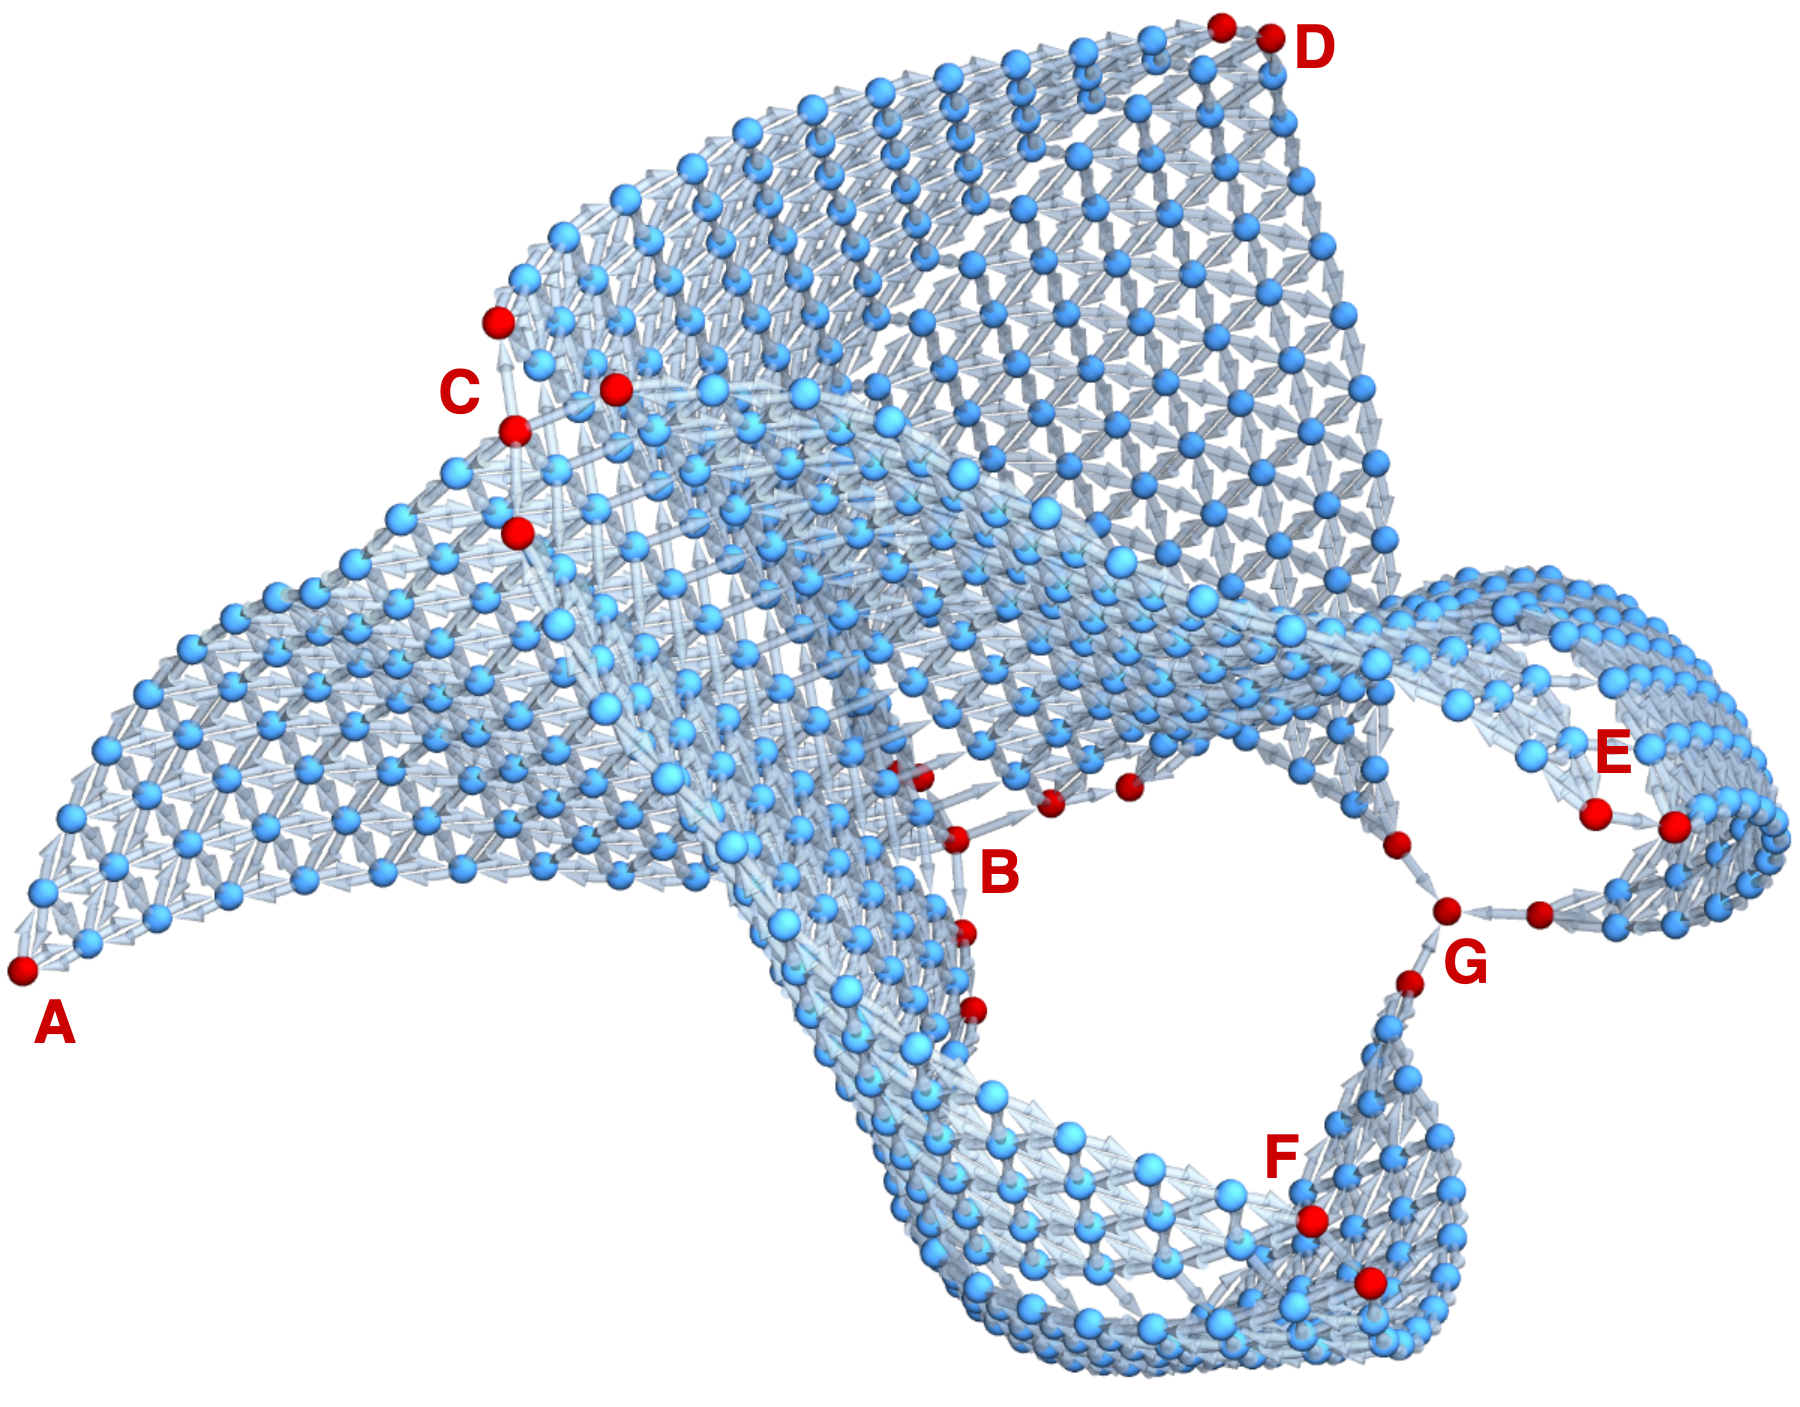
\includegraphics[width=0.57\textwidth]{nimplex/GraphComplex2.png}
    \end{adjustbox}
    \caption{Graph Complex Example \#2 depicting a problem where 3 choices (D/E/F) can be made to traverse from ABC to G through dual ternary systems containing B. Vertices were spread in 3D to depict three possible ABC to G paths, which would exactly overlap in a plane.} 
    \label{nimplex:fig:graphcomplex2}
\end{figure}

In the above examples in Figures~\ref{nimplex:fig:graphcomplex1}~and~\ref{nimplex:fig:graphcomplex2}, all connections between compositional spaces were directional; however, that is not necessary, and in some problems it may be beneficial to allow bidirectional movement. Suppose one tries to combine compositions A with D, which cannot be combined directly in any quantity, and also knows that (1) system ABC is highly feasible across it, but (2) system BCD is not traversable on its own. Thus, E can be introduced to set up intermediate spaces BDE and CDE, allowing obstacles in BCD to be avoided. Furthermore, BCE can also be set up as an alternative, possibly shortening the total path. Figure~\ref{nimplex:fig:graphcomplex3} depicts such a problem setup.

\begin{figure}[h]
    \centering
    \begin{adjustbox}{valign=c}
        \includegraphics[width=0.35\textwidth]{nimplex/GraphComplexMap3.png}
    \end{adjustbox}
    \hspace{6pt}
    \begin{adjustbox}{valign=c}
        \includegraphics[width=0.6\textwidth]{nimplex/GraphComplex3.png}
    \end{adjustbox}
    \caption{Graph Complex Example \#3 depicting the possibility of competing paths, including cycles.} 
    \label{nimplex:fig:graphcomplex3}
\end{figure}

Notably, while the above example in Figure~\ref{nimplex:fig:graphcomplex3} depicts a single 5th component E to help visualize cycling between spaces, these concepts can be extended to many possible intermediate components. At the same time, the maximum dimensionality of individual compositional spaces is kept constant ($d=3$). Thus, it provides a powerful method to keep the problem solvable, even experimentally, while considering many possible pathways formally defined prior to path planning to fit within the feasibility of evaluation and manufacturing.




\subsection{Discussion of Exploration} \label{nimplex:sec:discussion}

Critically, creating such a homogeneous problem structure through graph representation allows one to deploy the same exploration strategies across many dimensionalities and even combinations of individual spaces shown in Section~\ref{nimplex:ssec:complexes}. Furthermore, in the described graphs, points are on an equidistant grid; thus, it is easy to set up a heuristic function that can be both consistent and admissible. 

This, in turn, enables one to harvest many general-purpose graph traversal algorithms, which are actively researched and available through high-performance libraries. For instance, to navigate against constraints, the $A^*$ algorithm \cite{Hart1968APaths} can be used with such a heuristic and is mathematically guaranteed to find \textit{the} shortest feasible compositional path while exploring the least number of nodes \cite{Dechter1985GeneralizedA}, what can be critical if the shortest path is necessary while each evaluation is relatively expensive. Then, if one tries to find \emph{a} feasible solution first and then improve on it, modifications of the $A^*$ algorithms such as the $RWA^*$ \cite{Bhatia2021OnA} can be used to first make it more greedy and then gradually move towards $A^*$ to obtain the optimal solution if sufficient resources are available. Alternatively, for highly complex problems where exploration needs to proceed quickly towards the goal but the optimality guarantees are not needed, one can use a search algorithm based on the Monte Carlo tree search (MCTS), which has been famously used in conjunction with an ML model to master the game of Go \cite{Silver2016MasteringSearch}.



\section{Summary and Conclusion} \label{nimplex:sec:summary}

This work starts by providing an abstract description of compositional spaces applicable to a wide range of disciplines while formalizing several vital concepts. Then, Section~\ref{nimplex:ssec:compositionallycomplex} discusses complex compositional spaces, using Compositionally Complex Materials (CCMs) as a real-world application and considers the challenges of exploring such spaces using different methods. Section~\ref{nimplex:ssec:functionallygraded} uses another real-world application of Functionally Graded Materials (FGMs) to expand on that by discussing compositional spaces formed from compositions in other spaces and when these spaces are preferred for design. It also discusses key concepts related to path planning in relation to types of constraint and property optimizations. Last in the Introduction, Section \ref{nimplex:ssec:combinatorialcomplexities} discusses some equations critical to investigating the combinatorial complexities in these problems.

Next, discussions and implementations are given for several methods for efficiently solving compositional problems through random sampling in Section~\ref{nimplex:sec:randomuniformsampling}, grid-based methods in Section~\ref{nimplex:sec:simplexgrid}, graph-based methods, including graphs combining multiple compositional spaces, in Section~\ref{nimplex:sec:simplexgraph}. The three most critical contributions introduced in this process are:

\begin{enumerate}
    \item Novel algorithm for rapid procedural generation of \emph{N-dimensional graph representations} of compositional spaces where uniformly distributed simplex grid points in $d$ dimensions are completely connected to up to $d(d-1)$ neighbors representing all possible component-pair changes. For instance, in economics, this could represent all possible compositions of a financial portfolio of 12 assets and, for each one of them, all 132 transfer choices that can be made to modify it. Critically, this method scales linearly with the number of points and generates graphs with billions of connections between millions of points in just seconds. Furthermore, this algorithm allows deterministic memory allocation during the graph construction, where arrays of pointers to neighboring compositions represent allowed transitions, resulting in a very high-performance data structure.
    
    \item The new free, open-source software (FOSS) package \texttt{nimplex} (\href{https://nimplex.phaseslab.org}{nimplex.phaseslab.org}), which gives high-performance implementations of both essential existing methods and all new methods introduced within this work including the simplex graphs.
    
    \item The novel concept of combining many compositional spaces using graph representations to create homogeneous problem spaces, both simplifying the path planning and allowing for efficient incorporation of constraints and assumptions about problem spaces as demonstrated in Section~\ref{nimplex:ssec:complexes}. 
    
\end{enumerate}

In addition to the above, three other new contributions are given in this work:

\begin{enumerate}
    
    \item Sections~\ref{nimplex:sec:randomuniformsampling}~and~\ref{nimplex:sec:simplexgrid} discuss random sampling and grid construction in simplex spaces in the context of the composition of chemical spaces. In the process, several theoretical results critical to the problem, which have not been discussed previously in this context, are presented. For instance, the commonly found random sampling of a $d-1$ hypercube and rejection of compositions $>100\%$ to sample a $d$-component space, commonly found in software, has a rejection rate exhibiting factorial growth and can severely impact when deploying ML models.
    
    \item In Section~\ref{nimplex:ssec:internalgrid}, a new algorithm was developed to efficiently create internal (subspace-exclusive) grids in simplex spaces based on an algorithm from the literature (modified-NEXCOM \cite{Chasalow1995AlgorithmPoints}). It is beneficial to performance in cases of, for instance, sampling only $d$-component materials in $d$-component chemical space without considering lower-order points.

    \item In a few areas, Section~\ref{nimplex:ssec:functionallygraded} leverages its general character to go beyond the usual FGM literature introduction. For instance, it contrasts elemental spaces with attainable design spaces and discusses the use of similar compositions (alloy grades) in the design process to reduce cost and greenhouse emissions without making prior assumptions.
    
\end{enumerate}

\section{Code Availability} \label{nimplex:sec:code}

The \texttt{nimplex} software described in this work has been published as free open-source software (FOSS) under the MIT license. It can be effortlessly used as a \emph{native} Nim library, \emph{native} Python library, or Command Line Interface (CLI) tool interfacing with nearly any language through binary data or plain text.

All distributions of the source contain (1) the core library, (2) additional utilities, (3) testing procedures, (4) use examples, (5) quick-start guide using Python/CLI in the form of a Jupyter notebook, (6) \texttt{devcontainer.json} specification, and (7) documentation. They are available through:

\begin{itemize}
    \item The documentation page at \href{https://nimplex.phaseslab.org}{nimplex.phaseslab.org}, which contains (1) installation instructions, (2) usage instructions in Python, Nim, and CLI, and (3) Application Programming Interface (API) reference. It also links to a public GitHub repository hosting the latest code (\href{https://github.com/amkrajewski/nimplex}{github.com/amkrajewski/nimplex}) at the time of writing.

    % Not on arXiv
    %\item (Version X.X) As a supplement to this %manuscript, in the form of a ZIP file with both %(1) source code and (2) documentation HTML %files.

    % Reserved for now
    \item (Selected Major Versions) A public repository archive on Zenodo under DOI: \href{https://doi.org/10.5281/zenodo.10611931}{10.5281/zenodo.10611931}.
\end{itemize}


\printbibliography[heading=subbibintoc]




\newpage
\chapter*{Vita}
\thispagestyle{empty}

Adam Krajewski was born in Europe, where he spent his childhood and received pre-college education at a public school nationally recognized for its university-level chemistry curriculum. He first came to the United States in 2013 and moved entirely in 2015, joining the Materials Science and Engineering Department at Case Western Reserve University. Within the first two months of enrollment, he began research in Prof. Welsch's group, and started to take graduate courses in his sophomore year. Around the same time, he joined Prof. Willard's group, progressively moving from experiments towards theory, modeling, and simulations. In late 2016, he enrolled in graduate courses in Artificial Intelligence and specialize in applying Machine Learning to his research problems in Materials Science. 

After earning his B.S.E. degree in 2019, he moved directly to pursue PhD at Penn State under world-renowned thermodynamics expert Prof. Zi-Kui Liu and had the pleasure of working on implementing a variety of computational techniques, including machine learning, while having the support of colleagues who are specialists in ab-initio modeling, thermodynamic calculations, and materials discovery. Since 2022, he also extensively collaborated with LLNL and have spent two summers on-site at the lab.

\end{document}
